% document options %
\documentclass[11pt]{book}
%%

% used packages %
\usepackage{amsthm}
\usepackage{amsmath}
\usepackage[english,ngerman]{babel}
\usepackage{bbm}
\usepackage{bibgerm}
\usepackage{caption}
\usepackage{enumerate}
\usepackage{extarrows}
\usepackage[T1]{fontenc}
\usepackage[raiselinks=true,
  pdftex,colorlinks,bookmarks,
  bookmarks=true,
  bookmarksopenlevel=1,
  bookmarksopen=true,
  bookmarksnumbered=true,
  hyperindex=true,
  plainpages=false,
  pdfpagelabels=true,
  pdfborder={0 0 0.5}]{hyperref}
\usepackage[utf8]{inputenc}
\usepackage{listings}
\usepackage{multicol}
\usepackage{subfigure}
\usepackage{tabularx}
\usepackage{textcomp}
\usepackage[absolute,overlay]{textpos}
\usepackage{tikz}
\usetikzlibrary{calc}
\usetikzlibrary{decorations.pathreplacing}
\usepackage{vmargin}
%%

% debug packages %
% \usepackage{showframe}
%%

\lstset{%
	language=C,%
	basicstyle=\ttfamily,%
	keywordstyle=\bfseries,%
	showstringspaces=false%
}

% page layout %
\setmarginsrb{3cm}{1cm}{3cm}{1cm}{6mm}{7mm}{5mm}{15mm}
\marginparwidth 0mm
\marginparsep 0mm
\marginparpush 0pt
\columnwidth\textwidth
\setlength{\topsep}{0pt}
\setlength{\partopsep}{5pt plus 4pt minus 2pt}
%\setlength{\parindent}{5mm}
%%

% used helpers %
\hyphenation{
An-weis-ung
Au-then-ti-fi-ka-tions-in-for-ma-tion
aus-zu-lie-fern
Bei-spiel
bei-spiels-wei-se
Be-nut-zer
Be-nut-zer-grup-pe
Be-nut-zer-grup-pen
bei-spiels-wei-se
be-nö-ti-gen
be-nö-tig-ten
be-schrei-ben
Be-ur-tei-lung
be-zeich-net
be-züg-lich
Chif-frat
Chiffre-text-blöcke
De-chif-f-rie-rung
de-fi-nie-ren
durch-läuft
durch-lau-fen
Em-pfän-ger
Em-pfän-ger-sei-te
elek-t-ro-ma-g-ne-tisch
Feed-back
Ge-heim-hal-tung
Hard-ware
Hash-funk-tion
Hash-wert
Im-ple-men-tie-rung
Im-ple-men-tie-run-gen
ins-be-son-de-re
Klar-text
Kom-ple-men-tär-in-for-mation
Krypto-sys-tem
Krypto-sys-teme
Krypto-sys-temen
kryp-to-gra-phisch
Me-cha-nis-men
Men-schen-ver-stand
Nach-rich-ten
Nach-teil
Off-line
Pass-wort-hash-es
Perio-den-länge
Pro-zes-se
Puf-fer-grö-\ss en
Rück-wärts-hash-wert
Schie-be-re-gister-fol-ge
Schie-be-re-gister-fol-gen
Schie-be-re-gister-glei-chung
Schlü-sel
schlüs-sel-ab-hän-gi-g
schlüs-sel-ab-hän-gi-ge
schlüs-sel-ab-hän-gi-ger
schlüs-sel-ab-hän-gi-ges
schlüs-sel-ab-hän-gi-gen
Schlüs-sel-aus-tausch
Schlüs-sel-aus-tausch-ver-fah-ren
Schlüs-sel-zen-trale
Son-nen-stürme
si-che-ren
Si-cher-heits-ab-fra-gen
sinn-vol-len
Trans-for-ma-tions-re-gel
un-ter-schied-lich
un-ter-schied-li-che
un-ter-such-en
un-ter-sucht
Ver-än-de-run-gen
ver-blei-bende
Ver-schlüs-se-lung
Ver-schlüs-se-lungs-ver-fah-ren
Ver-schlüs-se-lungs-al-go-rith-mus
Ver-schlüs-se-lungs-stan-dard
Wör-ter-buch-an-griff
Wort-häu-fig-keit
Wort-häu-fig-kei-ten
Zer-ti-fi-kat-er-setz-ung
zu-ge-schrie-ben
Ver-schlüs-sel-ungs-stan-dard}
%%%%%%%%%%%%%%%%%%%%%%%%%%%%%%%%%%%%%%%%
%%% Makros für einheitliche Notation %%%
%%%%%%%%%%%%%%%%%%%%%%%%%%%%%%%%%%%%%%%%

\newcommand{\changefont}[3]{\fontfamily{#1} \fontseries{#2} \fontshape{#3} \selectfont}

%%% Notation für Gruppen, Ringe und Körper
\newcommand{\N}{\ensuremath{\mathbbm{N}}}
\newcommand{\No}{\ensuremath{\mathbbm{N}_0}}
\newcommand{\Z}[1]{\ensuremath{\mathbbm{Z}_{#1}}}
\newcommand{\Zx}[1]{\ensuremath{\mathbbm{Z}_{#1}^{\times}}}
\newcommand{\Q}{\ensuremath{\mathbbm{Q}}}
\newcommand{\R}{\ensuremath{\mathbbm{R}}}
\renewcommand{\P}{\ensuremath{\mathbbm{P}}}
\newcommand{\F}[1]{\ensuremath{\mathbbm{F}_{#1}}}
\newcommand{\Fx}[1]{\ensuremath{\mathbbm{F}_{#1}^{\times}}}
\newcommand{\K}{\ensuremath{\mathbbm{K}}}
\newcommand{\G}{\ensuremath{\mathbbm{G}}}
\newcommand{\Gx}{\ensuremath{\mathbbm{G}^{\times}}}

% For compatibility.
\newcommand{\calA}{\ensuremath{\mathcal{A}}}
\newcommand{\calC}{\ensuremath{\mathcal{C}}}
\newcommand{\calL}{\ensuremath{\mathcal{L}}}
\newcommand{\calO}{\ensuremath{\mathcal{O}}}
\newcommand{\calP}{\ensuremath{\mathcal{P}}}
\newcommand{\calR}{\ensuremath{\mathcal{R}}}
\newcommand{\calS}{\ensuremath{\mathcal{S}}}

%%% Notation für Kryptographie und Sonstiges
\newcommand{\plaint}{\ensuremath{M}}
\newcommand{\ciphert}{\ensuremath{C}}
\newcommand{\key}{\ensuremath{K}}
\newcommand{\skey}{\ensuremath{sk}}
\newcommand{\pkey}{\ensuremath{pk}}
\newcommand{\secpara}{\ensuremath{k}}
\newcommand{\enc}{\textsc{Enc}}
\newcommand{\dec}{\textsc{Dec}}
\newcommand{\sig}{\textsc{Sig}}
\newcommand{\ver}{\textsc{Ver}}
\newcommand{\keygen}{\textsc{KeyGen}}
\newcommand{\gen}{\textsc{Gen}}
\newcommand{\hash}{\ensuremath{h}}
\newcommand{\Com}{\textsc{Com}} %Commitment-Algorithmus
\newcommand{\A}{\ensuremath{\mathcal{A}}}
\newcommand{\advA}{\ensuremath{\mathcal{A}}}
\newcommand{\B}{\ensuremath{\mathcal{B}}}
\newcommand{\C}{\ensuremath{\mathcal{C}}}
\newcommand{\Sim}{\ensuremath{\mathcal{S}}} % Simulator
\newcommand{\ext}{\ensuremath{\mathcal{E}}} % Extraktor
\newcommand{\pw}{\ensuremath{\texttt{pw}}}

\newcommand\adv[2]{\mathbf{Adv}^{#1}_{#2}}
\DeclareMathOperator{\ggT}{ggT}
\DeclareMathOperator{\ggt}{ggT}
\newcommand*{\rArrow}{\ensuremath{\rightarrow}}
\newcommand*{\concat}{\ensuremath{\mathbin{\|}}} % Konkatenationssymbol %

\newcommand{\randUnif}{\xleftarrow{\textdollar}}

%Index-Macros

%Stromchiffren
\newcommand{\indexCaesarROT}{\index{ROT-13}}
\newcommand{\indexVignere}{\index{Vigenère-Chiffre}}
\newcommand{\indexCaesar}{\index{Caesar-Chiffre}}
\newcommand{\indexOTP}{\index{One-Time-Pad}}
\newcommand{\indexLFSR}{\index{Linear Feedback Shift Register (LFSR)}}

%Pseudozufall
\newcommand{\indexSeed}{\index{Seed|see {Pseudozufallszahlengenerator}}}
\newcommand{\indexPNS}{\index{Pseudozufallsfolge}}
\newcommand{\indexPRNG}{\index{Pseudozufallszahlengenerator}}

%Betriebsmodi
\newcommand{\indexECB}{\index{Betriebsmodus!Electronic Codebook Mode (ECB-Modus)}\index{Electronic Codebook Mode (ECB-Modus)}}
\newcommand{\indexCBC}{\index{Betriebsmodus!Cipher Block Chaining Mode (CBC-Modus)}\index{Cipher Block Chaining Mode (CBC-Modus)}}
\newcommand{\indexCTR}{\index{Betriebsmodus!Counter Mode (CTR-Modus)}\index{Counter Mode (CTR-Modus)}}

%Blockchiffren
\newcommand{\indexFeistel}{\index{Blockchiffre!Feistel networks}}
\newcommand{\indexDES}{\index{Blockchiffre!Data Encryption Standard (DES)}}
\newcommand{\indexTwoDES}{\index{Blockchiffre!2DES}}
\newcommand{\indexThreeDES}{\index{Blockchiffre!Triple Data Encryption Standard (3DES)}}
\newcommand{\indexAES}{\index{Blockchiffre!Advanced Encryption Standard (AES)}}
\newcommand{\indexConfusion}{\index{Confusion}}
\newcommand{\indexDiffusion}{\index{Diffusion}}
\newcommand{\indexSBOX}{\index{Substitution-Box (S-Box)}}

\newcommand{\indexIV}{\index{Initialisierungsvektor (IV)}}


\newcommand{\indexSecParam}{\index{Sicherheitsparameter}}

\newcommand{\indexNegl}{\index{Vernachlässigbarkeit}}

\newcommand{\indexINDCPA}{\index{Indistinguishability under chosen-plaintext attacks (IND-CPA)}}
\newcommand{\indexINDCCA}{\index{Indistinguishability under chosen-ciphertext attacks (IND-CCA)}}

\newcommand{\indexKeyExchange}{\index{Schlüsselaustausch}}

\newcommand{\indexOracle}{\index{Orakel}}

%Angriffe
\newcommand{\indexAttack}{\index{Angriff}}
\newcommand{\indexBruteForce}{\index{Angriff!Brute-Force / Exhaustive Search}}
\newcommand{\indexMeetInTheMiddle}{\index{Angriff!Meet-in-the-Middle}}
\newcommand{\indexManInTheMiddle}{\index{Angriff!Man-in-the-Middle}}
\newcommand{\indexDOS}{\index{Angriff!Denial of Service (DOS)}}
\newcommand{\indexLinCrypt}{\index{Lineare Kryptoanalyse}\index{Angriff!Lineare Kryptoanalyse}\index{Kryptoanalyse!Lineare Kryptoanalyse}}
\newcommand{\indexDiffCrypt}{\index{Differentielle Kryptoanalyse}\index{Angriff!Differentielle Kryptoanalyse}\index{Kryptoanalyse!Differentielle Kryptoanalyse}}
\newcommand{\indexBirthDayAttack}{\index{Angriff!Birthday-Angriff}}

\newcommand{\indexCryptAnalysis}{\index{Kryptoanalyse}}

%Angreifer
\newcommand{\indexAdv}{Angreifer}
\newcommand{\indexPassiveAdv}{\index{Angreifer!Passiv}}
\newcommand{\indexActiveAdv}{\index{Angreifer!Aktiv}}
\newcommand{\indexEfficientAdv}{\index{Angreifer!Effizient}}
\newcommand{\indexPPTAdv}{\index{Angreifer!Probabilistic Polynomial Time (PPT)}}

%Hashfunktionen
\newcommand{\indexHashFunction}{\index{Hashfunktion|see {Kryptographische Hashfunktion}}}
\newcommand{\indexCryptHashFunction}{\index{Kryptographische Hashfunktion}}
\newcommand{\indexCollisionResistance}{\index{Kryptographische Hashfunktion!Kollisionsresistenz}\index{Kollisionsresistenz}}
\newcommand{\indexPreImageResistance}{\index{Kryptographische Hashfunktion!Einwegeigenschaft}\index{Einwegeigenschaft}}
\newcommand{\indexTargetCollisionResistance}{Kryptographische Hashfunktion!Target Collision Resistance}\index{Target Collision Resistance}

\newcommand{\indexMDTransformation}{\index{Merkle-Damgård-Transformation}}

\newcommand{\indexMDFive}{\index{MD-5}}

%SHA
\newcommand{\indexSHA}{\index{Secure Hash Algorithm (SHA)}}
\newcommand{\indexSHAOne}{Secure Hash Algorithm (SHA)!SHA-1}
\newcommand{\indexSHATwo}{Secure Hash Algorithm (SHA)!SHA-2}
\newcommand{\indexSHAThree}{Secure Hash Algorithm (SHA)!SHA-3}

\newcommand{\indexEncryptionSymm}{\index{Verschlüsselung!symmetrisch}}
\newcommand{\indexEncryptionAsymm}{\index{Verschlüsselung!asymmetrisch}}

%RSA
\newcommand{\indexRSA}{\index{RSA}}
\newcommand{\indexRSATextBook}{\index{RSA!Textbook}}
\newcommand{\indexRSAOAEP}{\index{RSA!Optimal asymmetric encryption padding (OAEP)}}
\newcommand{\indexEEA}{\index{Erweiterter Euklidischer Algorithmus (EEA)}}
\newcommand{\indexEulerPhiFunction}{\index{Eulersche Phi-Funktion}}
\newcommand{\indexFermatLittleTheorem}{\index{Fermat!Kleiner Satz}}
\newcommand{\indexChineseRemainderTheorem}{\index{Chinesischer Restsatz}}
\newcommand{\indexRandomOracleModel}{\index{Random Oracle Model}}

%ElGamal
\newcommand{\indexElGamal}{\index{ElGamal}}
\newcommand{\indexDLOGProblem}{\index{DLOG-Problem}}
\newcommand{\indexDecisionalDiffieHellman}{\index{Decisional Diffie-Hellman-Annahme (DDH-Annahme)}}
\newcommand{\indexMessageTransformation}{\index{ElGamal!Nachrichtenumwandlung}}
\newcommand{\indexHashElGamal}{\index{Hash-ElGamal}}

%Authentifikation
\newcommand{\indexMessageAuthSymm}{\index{Nachrichtenauthentifikation!symmetrisch}}
\newcommand{\indexMessageAuthAsymm}{\index{Nachrichtenauthentifikation!asymmetrisch}}
\newcommand{\indexMAC}{\index{Message Authentication Code (MAC)}}
\newcommand{\indexHMAC}{\index{Keyed-Hash Message Authentication Code (HMAC)}}
\newcommand{\indexEUFCMA}{\index{Existential unforgeability under adaptive chosen message attacks (EUF-CMA)}}

\newcommand{\indexSig}{\index{Signatur}}

\newcommand{\indexPRF}{\index{Pseudorandomisierte Funktion (PRF)}}
\newcommand{\indexHashSign}{\index{Hash-then-Sign}}


\def\dh{d.\,h.\ }

%%% Umgebungen

\theoremstyle{plain}

\newtheorem{theorem}{Theorem}[chapter]
\newtheorem*{beweis}{Beweis}
\newtheorem*{beweisidee}{Beweisidee}
\newtheorem{beispiel}[theorem]{Beispiel}

\theoremstyle{definition}

\newtheorem{definition}[theorem]{Definition}
%%

% content %
\title{Sicherheit}
\author{IKS}

\setcounter{tocdepth}{4}
\setcounter{secnumdepth}{5}

\begin{document}
\frontmatter

\newcommand{\diameter}{20}
\newcommand{\xone}{-15}
\newcommand{\xtwo}{160}
\newcommand{\yone}{15}
\newcommand{\ytwo}{-253}

\begin{titlepage}

\begin{tikzpicture}[overlay]
\draw[color=gray]
		 (\xone mm, \yone mm)
  -- (\xtwo mm, \yone mm)
 arc (90:0:\diameter pt)
  -- (\xtwo mm + \diameter pt , \ytwo mm)
	-- (\xone mm + \diameter pt , \ytwo mm)
 arc (270:180:\diameter pt)
	-- (\xone mm, \yone mm);
\end{tikzpicture}


\begin{textblock}{10}[0,0](4,2.5)
  
\includegraphics[width=.3\textwidth]{logos/KITLogo.pdf}
\end{textblock}
\changefont{phv}{m}{n}
\vspace*{3cm}
\begin{center}
  \LARGE{Skript zur Stammvorlesung}
  \vspace*{1.5cm}\\
  \Huge{Sicherheit}\\
  \vspace*{3cm}
  \Large{\textbf{Karlsruher Institut für Technologie}\\
  \vspace*{6mm}
  Fakultät für Informatik\\
  \vspace*{4mm}
  Institut für Theoretische Informatik\\
  Arbeitsgruppe für Kryptographie und Sicherheit}\\
  
  \vspace*{2cm}
  Die aktuelle Version des Skriptes befindet sich noch im Aufbau, daher kann weder für Vollständigkeit noch Korrektheit garantiert werden. Hinweise zu Fehlern, Kritik und Verbesserungsvorschläge nehmen wir per Mail an \url{skript-sicherheit@ira.uka.de} entgegen.
  
  \vspace*{2cm}
  Letzte Änderung: \today
\end{center}


\begin{textblock}{10}[0,0](4,16.8)
\tiny{
  \iflanguage{english}
  {KIT -- University of the State of Baden-Wuerttemberg and National Laboratory of the Helmholtz Association}
  {KIT -- Universität des Landes Baden-Würtemberg und nationales Forschungszentrum der Helmholtz-Gesellschaft}
}
\end{textblock}

\begin{textblock}{10}[0,0](14,16.75)
\large{
  \textbf{www.kit.edu}
}
\end{textblock}

\end{titlepage}

\thispagestyle{empty}
\ \vfill
\begin{flushleft}
  Copyright $\copyright$ ITI und Verfasser 2014\\
  \ \\
  Karlsruher Institut für Technologie\\
  Institut für Theoretische Informatik\\
  Arbeitsgruppe für Kryptographie und Sicherheit\\
  Am Fasanengarten 5\\
  76131 Karlsruhe
\end{flushleft}
\newpage


\tableofcontents

\mainmatter

\chapter{Einleitung}
\label{cha:intro}

\section{Was ist Sicherheit?}
Sicherheit bedeutet, dass Schutz geboten wird. Was wird geschützt? Vor wem? Wie wird es geschützt? Wer schützt? Es gibt zwei verschiedene Ansätze, die beide unter den deutschen Begriff \emph{Sicherheit} fallen: \emph{Betriebssicherheit} (engl. safety) und \emph{Angriffsicherheit} (engl. security).
\begin{description}
	\item[Betriebssicherheit:] 
	Unter \emph{Betriebssicherheit} versteht man die Sicherheit einer Situation, die von einem System geschaffen wird: Ist der Betrieb eines Systems sicher? Das bedeutet vor allem, dass keine externen Akteure betrachten werden: Niemand manipuliert das System! Diese Art von Sicherheit wird mit Methoden erreicht, die wahrscheinliche Fehlerszenarien abdecken und verhindern. Beispiele für Systeme, die uns Betriebssicherheit gewähren, sind Arbeitsschutzkleidung zur Vermeidung von Arbeitsunfälle, Backup-Systeme zur Vorbeugung gegen den Ausfall von Komponenten oder elektrische Sicherungen, um uns vor gefährlichen Kurzschlussströmen zu schützen.
	\item[Angriffssicherheit:] 
	Unter \emph{Angriffssicherheit} versteht man die Sicherheit eines Systems in Bezug auf das externe Hinzufügen von Schäden: Ist es möglich, das System von Außen zu manipulieren? Anders als bei \emph{Betriebssicherheit} betrachten wir keine Schäden, die durch den aktuellen Zustand des Systems entstehen können. Wir betrachten Schäden die von einem externen Akteur, im folgenden \emph{Angreifer} genannt, ausgehen. Dabei gehen wir davon aus, dass ein Angreifer Schwachstellen des Systems gezielt sucht und verwendet. Aus diesem Grund genügt es nicht, wahrscheinliche Fehlerszenarien zu betrachten. Es ist vielmehr nötig, alle Angriffsmöglichkeiten zu unterbinden. Beispiele für diese Art von Sicherheit sind gepanzerte Fahrzeuge, Türschlösser gegen Einbrecher und Wasserzeichen, um das Fälschen von Banknoten zu erschweren.
\end{description}
In dieser Vorlesung beschäftigen wir uns ausschließlich mit dem Konzept der Angriffssicherheit. Darüber hinaus beschäftigen wir uns nur mit dem Schutz informationstechnischer Systeme.

\section{Grundlagen}
Betrachten wir ein informationstechnisches System. Es existierten zahlreiche Arten von Attacken, vor denen wir uns durch verschiedene Techniken schützen müssen. Es ist selten hilfreich, das Gesamtsystem als Einheit zu betrachten. Dafür ist es einfach zu komplex. Stattdessen zerlegen wir es in kleinere "`Bausteine"', für deren Sicherheit wir einzeln garantieren können. Diese Vorlesung stellt die wichtigsten Bausteine vor. In diesem Abschnitt geben wir einen Überblick über die wichtigsten Grundbegriffe. Im Anschluss werden wir stets auf die weiterführenden Kapitel verweisen.

\subsection{Verschlüsselung}

Ziel der Verschlüsselung ist es, Informationen auf eine bestimmte Personengruppe zu begrenzen. Stellen wir uns vor, ein Sender Bob möchte eine Nachricht an eine Empfängerin Alice übermitteln. Die Nachricht ist privat, doch Eve lauscht. Können Alice und Bob kommunizieren, ohne das Eve sinnvolle Informationen erhält? Wie?

Ein Verschlüsselungsverfahren (\emph{Chiffre}) besteht aus einer oder mehreren mathematischen Funktionen, die zur Ver- und Entschlüsselung einer Nachricht eingesetzt werden. Bei der Verschlüsselung wird ein Klartext (eine \emph{Nachricht}) in einen Geheimtext (ein \emph{Chiffrat}) umgewandelt. Das Chiffrat soll einem unautorisierten Dritten keine Informationen über die Nachricht offenbaren. Das Chiffrat kann dann durch Entschlüsselung wieder in den Klartext umgewandelt werden. Verschlüsselung wird auch als \emph{Chiffrierung}, Entschlüsselung als \emph{Dechiffrierung} bezeichnet.

In heutigen Algorithmen wird zur Chiffrierung und Dechiffrierung noch eine weitere Information, der \emph{Schlüssel}, benutzt. Diese Situation ist in Abbildung~\ref{fig:encryption:principle} dargestellt. Ist der Schlüssel für Ver- und Entschlüsselung gleich, so spricht man von einem \emph{symmetrischen} Verfahren. Sind die Schlüssel verschieden, handelt es sich um ein \emph{asymmetrisches} Verfahren. Symmetrische Verfahren werden in \autoref{cha:symencryption} vorgestellt, asymmetrische Verfahren in \autoref{ch:asymmenc}. Klartext und Chiffrat können aus beliebigen Zeichen bestehen. Im Kontext computergestützter Kryptographie sind beide normalerweise binär kodiert.

Für den Fall, dass Bob seine Nachricht an Alice vor dem Senden verschlüsselt, können die beiden ihre Kommunikation vor Eve verbergen. Im Gegensatz zu Eve sollte Alice die Nachricht natürlich entschlüsseln können. Ein Chiffrat muss jedoch nicht immer versendet werden. Es kann auch zu Speicherung auf einem Datenträger vorgesehen sein.
\begin{figure}[h]
	\begin{center}
		\unitlength=1mm
		\linethickness{0.4pt}
		\begin{picture}(120,20)
			\put(0,5){\vector(1,0){20}}
			\put(10,6){\makebox(0,0)[cb]{$\plaint$}}
			\put(35,15){\vector(0,-1){7.5}}
			\put(38,10){\makebox(0,0)[cb]{$\key$}}
			\put(20,2.5){\framebox(30,5){\enc}}
			\put(50,5){\vector(1,0){20}}
			\put(60,6){\makebox(0,0)[cb]{$\ciphert$}}
			\put(85,15){\vector(0,-1){7.5}}
			\put(88,10){\makebox(0,0)[cb]{$\widetilde{\key}$}}
			\put(70,2.5){\framebox(30,5){\dec}}
			\put(100,5){\vector(1,0){20}}
			\put(110,6){\makebox(0,0)[cb]{$\plaint$}}
		\end{picture}
	\end{center}
	\caption{$\mathrm{\dec_{\widetilde{\key}}(\enc_\key(\plaint))= \plaint}$. Falls $\key = \tilde{\key}$ handelt es sich um ein symmetrisches
Verschlüsselungsverfahren, ist $\key \neq \tilde{\key}$, so ist es ein asymmetrisches Verfahren.}
	\label{fig:encryption:principle}
\end{figure}

\noindent Üblicherweise benutzen wir folgende Abkürzungen:\\

\begin{center}
	\begin{tabular}{ l l l }
		Nachricht: & \plaint\ & (engl. \emph{message})\\
		Chiffrat: & \ciphert\ & (engl. \emph{ciphertext})\\
		Schlüssel: & \key\ & (engl. \emph{key})\\
		Chiffrierung: & \enc\ & (engl. \emph{encryption})\\
		Dechiffrierung: & \dec\ & (engl. \emph{decryption})\\
	\end{tabular}
\end{center}

\subsubsection{Geheime Verfahren}

Zwar gibt es eine ganze Reihe von Verschlüsselungsverfahren ohne Schlüssel, allerdings hängt deren Sicherheit allein davon ab, dass der Algorithmus geheim bleibt. Im Kontext von Algorithmen, deren Sicherheit auf der Geheimhaltung des Verfahren beruht, spricht man auch von \emph{security by obscurity}. Solche Algorithmen sind unflexibel und aus heutiger Sicht unsicher. Sie sind daher eher von historischem Interesse und werden im Folgenden nicht näher betrachtet. Stattdessen hat sich Kerckhoffs' Prinzip etabliert.

\subsubsection{Kerckhoffs' Prinzip}

Kerckhoffs' Prinzip ist ein Grundsatz moderner Kryptographie. Er wurde im 19. Jahrhundert von Auguste Kerckhoffs formuliert \cite{Kerckhoffs}.
\begin{quote}
	\grqq{}The cipher method must not be required to be secret, and it must be able to fall into the hands of the enemy without inconvenience.\grqq
\end{quote}
Anders ausgedrückt darf die Sicherheit eines Verschlüsselungsverfahren nur von der Geheimhaltung des Schlüssels und nicht von der Geheimhaltung des Algorithmus abhängen.
Kerckhoffs' Prinzip findet in den meisten heutigen Verschlüsselungsverfahren Anwendung. Gründe dafür sind:
\begin{itemize}
	\item Es ist einfacher, einen Schlüssel als einen Algorithmus geheim zu halten.
	\item Es ist einfacher, einen kompromittierten Schlüssel zu ersetzen, statt einen ganzen Algorithmus zu tauschen. Tatsächlich ist es gängige Sicherheitspraxis, den Schlüssel regelmäßig zu wechseln, selbst wenn dieser nicht bekannt geworden ist.
	\item Bei vielen Teilnehmerpaaren (z.B. innerhalb einer Firma) ist es um einiges einfacher, unterschiedliche Schlüssel zu verwenden, statt unterschiedliche Algorithmen für jede Kombination zu entwerfen.
	\item Veröffentlichte Verfahren können von vielen Fachleuten untersucht werden, wodurch eventuelle Fehler wahrscheinlicher auffind- und behebbar sind.
	\item Da der Schlüssel keinen Teil des Algorithmus (bzw. seiner Implementierung) darstellt, ist er im Gegensatz zum Algorithmus nicht anfällig gegen Reverse-Engineering.
	\item Öffentliche Entwürfe ermöglichen die Etablierung von Standards.
\end{itemize}
Diese Gründe mögen einleuchtend sein. Trotzdem wurde Kerckhoffs' Prinzip immer wieder zugunsten geheimer Verfahren ignoriert, was zu fatalen Ergebnissen führte. Es sollten nur standardisierte und öffentlich getestete Verfahren verwendet werden.

\chapter{Symmetrische Verschlüsselung}
\label{cha:symencryption}
Ein symmetrisches Verschlüsselungsverfahren sichert eine Kommunikation zwischen (typischerweise zwei) Parteien durch einen geheimen Schlüssel, den alle Parteien kennen. Der Schlüssel dient sowohl der Chiffrierung als auch der Dechiffrierung. Er wird keiner bestimmten Partei, sondern einer bestimmten Kommunikationsverbindung zugeordnet. Alle klassischen Verschlüsselungsverfahren sind symmetrisch.

Um eine sichere Kommunikation zu beginnen, müssen sich beide Parteien zuvor auf einen gemeinsamen Schlüssel einigen. Diesen Vorgang nennen wir \emph{Schlüsselaustausch}. Bei \emph{offenen} digitalen Systemen, wie dem Internet, können wir nicht davon ausgehen, dass die Kommunikationspartner schon vorher in Kontakt standen: Prinzipiell kann jeder an einem offenen System teilnehmen und hat Zugriff auf die im System angebotenen Dienste. Daher muss der Schlüsselaustausch innerhalb des Systems selbst erfolgen. Schlüsselaustauschverfahren betrachten wir allerdings erst in Kapitel~\ref{cha:keyexchange} und gehen, der Einfachheit halber, zunächst davon aus, dass beide Kommunikationspartner bereits über einen gemeinsamen geheimen Schlüssel verfügen.

Eine Verschlüsselungsfunktion erwartet in der Regel eine Eingabe fester Länge. Daher wird ein Klartext beliebiger Länge vor der Verarbeitung in eine Folge von Blöcken oder Zeichen fester Länge aufgeteilt, die dann einzeln chiffriert werden. Wird für jeden Block die Verschlüsselungsoperation mit dem selben Schlüssel verwendet, so spricht man von \emph{Blockchiffren}. Diese werden in Kapitel~\ref{sec:blockchiffren} ausführlich behandelt. Als \emph{sequentielle Chiffren} oder \emph{Stromchiffren} bezeichnet man Verschlüsselungsverfahren, bei denen die Klartextzeichen nacheinander mit einem in jedem Schritt variierenden Element eines Schlüsselstroms kombiniert werden.

\section{Stromchiffren}
Wir können einen Klartext $\plaint$ als eine endliche Folge $\plaint = (\plaint_i) = (\plaint_1,\plaint_2,\ldots,\plaint_n) $ von Zeichen $\plaint_i$ aus einem Klartextalphabet auffassen. Eine Stromchiffre verschlüsselt einen Klartext, indem sie jedes Klartextzeichen $\plaint_i$ durch ein Chiffratzeichen $\ciphert_i$ aus einem Chiffratalphabet in geeigneten Weise ersetzt. Dabei wird dasselbe Klartextzeichen an verschiedenen Positionen nicht notwendigerweise durch das gleiche Chiffratzeichen codiert: Im Allgemeinen folgt für $i \ne j$ aus $\plaint_i = \plaint_j$ nicht $\ciphert_i = \ciphert_j$. Eine derartige Zeichenersetzung nennt man auch \emph{polyalphabetische Substitution}. An dieser Stelle sei erwähnt, dass eine Stromchiffre nicht auf dem ursprünglichen Alphabet des Klartextes arbeiten muss. Sie verwendet jedoch elementare Einheiten "`kleiner"' Länge, aus denen der Klartext durch Konkatenation aufgebaut werden kann. Solche Einheiten nennen wir im Folgenden Zeichen.

In den meisten Fällen wird die Verschlüsselungsfunktion $\enc$  mit einer einfachen Funktion realisiert, die unabhängig vom Schlüssel ist. Bei binären Klartextströmen findet häufig die XOR"=Funktion Anwendung; der Schlüsselstrom wird also bitweise modulo 2 zum entsprechenden Teil des Klartextes hinzuaddiert und wir schreiben $\ciphert_i = \plaint_i\oplus\key'_i$. Der Schlüsselstrom $\key' = (\key'_i) = (\key'_1,\key'_2,\ldots,\key'_n)$ wird dabei durch einen Generator $G$ aus dem Schlüssel $\key$ erzeugt. Das Verfahren ist in Abbildung~\ref{fig:streamcipher} dargestellt.

\begin{figure}[h]
	\centering
	\unitlength=1mm
	\linethickness{0.4pt}
	\begin{picture}(70,50)
		\put(5,5){\makebox(0,0)[cc]{$\plaint_i$}}
		\put(10,5){\vector(1,0){20}}
		\put(31,2){\framebox(8,6)[cc]{$\enc$}}
		\put(40,5){\vector(1,0){20}}
		\put(65,5){\makebox(0,0)[cc]{$\ciphert_i$}}
		\put(35,20){\vector(0,-1){10}}
		\put(35,13){\makebox(6,6)[cc]{$\key'_i$}}
		\put(32,22){\framebox(6,6)[cc]{$G$}}
		\put(35,40){\vector(0,-1){10}}
		\put(35,45){\makebox(0,0)[cc]{$\key$}}
	\end{picture}
	\caption{Prinzip einer Stromchiffre. Der Klartextstrom $(\plaint_1,\plaint_2,\ldots,\plaint_n)$ wird zeichenweise mit einem, aus dem Schlüssel $\key$ mit
	Generator $G$ erzeugten, Schlüsselstrom $(\key'_1, \key'_2, \ldots, \key'_n)$ durch $\enc$ verschlüsselt.}
	\label{fig:streamcipher}
\end{figure}

Das klassische Beispiel einer Stromchiffre ist die in Abschnitt~\ref{ssec:vigenere} vorgestellte \emph{Vigen\`ere"=Chiffre}. Im Gegensatz zur Vigen\`ere"=Chiffre bietet eine Stromchiffre, die auf einer wirklich zufälligen Schlüsselfolge basiert, perfekte Geheimhaltung der verschlüsselten Nachricht. Dieses Verfahren heißt \emph{One-Time-Pad} und wird im Abschnitt~\ref{ssec:otp} vorgestellt.

\subsection{Caesar-Chiffre}
Eine der ersten schriftlich belegten Chiffren ist die \emph{Caesar-Chiffre}. Der Name stammt vom römischen Feldherrn \emph{Julius Caesar}, der nach Aufzeichnungen des römischen Schriftstellers \emph{Sueton} seine militärische Korrespondenz verschlüsselte, indem er jeden Buchstaben des Klartextalphabets um 3 nach rechts verschob.

\begin{table}[h]
	\centering
	\setlength{\tabcolsep}{2pt}
	\begin{tabular}{l*{26}{c}}
		Klartextalphabet: &A&B&C&D&E&F&G&H&I&J&K&L&M&N&O&P&Q&R&S&T&U&V&W&X&Y&Z\\
		Geheimtextalphabet: &D&E&F&G&H&I&J&K&L&M&N&O&P&Q&R&S&T&U&V&W&X&Y&Z&A&B&C\\
	\end{tabular}
	\caption{Beispiel der Caesar-Chiffre}
\end{table}

Aus dem Klartext \glqq CHIFFRE\grqq{} wird damit beispielsweise das Chiffrat \glqq FKLIIUH\grqq. Zur Entschlüsselung werden die Buchstaben im Geheimtextalphabet entsprechend um 3 nach links verschoben. Das Problem bei dieser Art von Verschlüsselung ist unmittelbar ersichtlich: Die Methode verändert sich nicht. Daher kann jeder, der einmal erkannt hat, wie Caesar seine Nachrichten verschlüsselte, diese ohne Probleme entschlüsseln. Es gibt keinen Schlüssel und die Sicherheit des Verfahrens hängt allein von der Geheimhaltung der Chiffre ab.

Manchmal wird auch die allgemeine \emph{Verschiebe-Chiffre} als Caesar-Chiffrierung bezeichnet. Bei dieser Chiffre gibt es einen Schlüssel, der die Anzahl der Stellen angibt, um die verschoben wird. Für die Verschlüsselung gilt dann $\enc_\key(\plaint_i) = (\plaint_i + \key)\ mod\ 26$ und für die Entschlüsselung dementsprechend $\dec_\key(\ciphert_i) = (\ciphert_i - \key)\ mod\ 26$. Da allerdings nur 26 mögliche Schlüssel existieren, ist es selbst ohne Computerunterstützung möglich, jeden Schlüssel auszuprobieren. Ein solcher Angriff wird als \emph{exhaustive search} oder \emph{Brute-Force-Angriff} bezeichnet.

\begin{figure}[h]
	\centering
	\unitlength=1mm
	\linethickness{0.4pt}
	\begin{picture}(100,30)
		\put(5,5){\makebox(0,0)[cc]{$\plaint_i$}}
		\put(10,5){\vector(1,0){20}}
		\put(32,2){\framebox(35,6)[cc]{$(\plaint_i + \key) \mod 26$}}
		\put(70,5){\vector(1,0){20}}
		\put(95,5){\makebox(0,0)[cc]{$\ciphert_i$}}
		\put(50,20){\vector(0,-1){10}}
		\put(47,22){\makebox(6,6)[cc]{$\key$}}
	\end{picture}
	\caption{Prinzip einer Verschiebe-Chiffre. Der Klartextstrom $(\plaint_1,\plaint_2,\ldots,\plaint_n)$ wird zeichenweise um den Schlüssel $\key \in \{ 1,\ldots,26\}$ verschoben.}
	\label{fig:caesarcipher}
\end{figure}

Diese Beobachtung führt zu dem wichtigen Prinzip, dass jedes sichere Verschlüsselungsverfahren einen Schlüsselraum besitzen muss, der nicht durch exhaustive search angreifbar ist. Im heutigen Zeitalter, in dem für einen Brute-Force-Angriff ein Netz aus mehreren tausend Computern benutzt werden können, muss die Anzahl der möglichen Schlüssel sehr groß sein (mindestens $2^{90}$ \cite{report:minkeylength}). Es ist jedoch wichtig zu verstehen, dass das obige Prinzip lediglich eine notwendige und keine hinreichende Bedingung für ein sicheres Verschlüsselungsverfahren darstellt.

Interessanterweise ist eine Variante der Caesar-Verschlüsselung heute weit verbreitet. Sie wird \emph{ROT-13} genannt und führt eine Verschiebung
um 13, anstatt um 3 Stellen durch. Es ist bekannt, dass diese Art von Verschlüsselung keine kryptographische Sicherheit bietet. ROT-13 wird lediglich dazu
verwendet, Spoiler oder Pointen bis zu einer bewussten Entschlüsselung zu verschleiern. Der Vorteil von ROT-13 besteht darin, dass Ver- und
Entschlüsselung exakt die selbe Funktion verwendet, was für eine einfach Implementierung sorgt.

\subsection{Vigen\`ere-Chiffre}
\label{ssec:vigenere}
Eine Weiterentwicklung der Caesar-Chiffre, die mehr Sicherheit bietet, ist die sogenannte Vigen\`ere-Chiffre, benannt nach einem Franzosen des
sechzehnten Jahrhunderts, \emph{Blaise de Vigen\`ere}. Der Unterschied zur Caesar-Chiffre besteht darin, dass nicht ein konstanter Schlüssel (und damit ein
einzelnes Alphabet) zur Chiffrierung jedes einzelnen Zeichens verwendet wird, sondern eine (möglichst lange) Folge von Schlüsseln. Der Zeichenvorrat ist das
lateinische Alphabet mit seinen 26 Buchstaben. Die Verknüpfung der Schlüsselfolge mit der Klartextfolge geschieht durch die zeichenweise Addition modulo~26.
Als Schlüsselwort dient eine periodisch wiederkehrende Zeichenfolge. Erst das Wiederholen einer im Verhältnis zum Klartext kurzen Schlüsselfolge
ermöglicht die Kryptoanalyse des Vigen\`ere"=Systems.

\begin{table}[h]
	\centering
	\setlength{\tabcolsep}{2pt}
	\begin{tabular}{ll}
		Schlüssel: 
		& SICHER
	\end{tabular}
	\begin{tabular}{l*{26}{c}}
		Klartext:
		&A&B&C&D&E&F&G&H&I&J&K&L&M&N&O&P&Q&R&S&T&U&V&W&X&Y&Z\\
		Schlüsselfolge:
		&S&I&C&H&E&R&S&I&C&H&E&R&S&I&C&H&E&R&S&I&C&H&E&R&S&I\\
		Geheimtext:
		&T&K&F&L&J&X&Z&Q&L&R&P&D&F&W&R&X&V&J&L&C&X&D&B&P&R&I\\
	\end{tabular}
	\caption{Beispiel einer Vigen\`ere-Chiffre}
\end{table}
\clearpage

\begin{figure}[h]
	\centering
	\unitlength=1mm
	\linethickness{0.4pt}
	\begin{picture}(100,50)
		\put(5,5){\makebox(0,0)[cc]{$\plaint_i$}}
		\put(10,5){\vector(1,0){20}}
		\put(32,2){\framebox(35,6)[cc]{$(\plaint_i + \key'_i) \mod{} 26$}}
		\put(70,5){\vector(1,0){20}}
		\put(95,5){\makebox(0,0)[cc]{$\ciphert_i$}}
		\put(50,20){\vector(0,-1){10}}
		\put(50,13){\makebox(6,6)[cc]{$\key'_i$}}
		\put(30,22){\framebox(40,6)[cc]{$\key'_i = \key_{((i - 1) \mod{} l) + 1}$}}
		\put(50,40){\vector(0,-1){10}}
		\put(50,45){\makebox(0,0)[cc]{$\key$}}
	\end{picture}
	\caption{Prinzip einer Vigen\`ere"=Chiffre. Der Schlüsselstrom $\key_i'$ entsteht durch Wiederholung des Schlüssels $\key$: $\key'_i =
\key_{((i - 1) \;  \mod{}  \; l) + 1}$, wobei $l$ die Länge des Schlüssels $\key$ ist. Der Klartextstrom $(\plaint_1,\plaint_2,\ldots,\plaint_n)$ wird zeichenweise, entsprechend der Verschiebe-Chiffre, mit dem passenden Buchstaben des Schlüsselstroms verschlüsselt.}
	\label{fig:vigerecipher}
\end{figure}

\begin{figure}[h]
	Ist $\underline k = (k_1,\ldots,k_{l})$ eine Schlüsselfolge der Länge $l$, so ist die Chiffrierabbildung der Vigen\`ere-Chiffre gegeben durch:
	\begin{equation*}
		E_{\underline k} : m_1\ldots m_{r} \mapsto t_{k_1}(m_1)\ldots t_{k_{l}}(m_{l})t_{k_1}(m_{l+1})\ldots t_{k_{r\bmod{l}}}(m_{r})
	\end{equation*}
	\begin{equation*}
		\begin{array}{rp{14cm}}
	    		{\rm mit\colon\ }		& $m_1\ldots m_{r}$ Klartextfolge der Länge $r$ und\\
							& $t_{k_j}(m_i) := m_i + k_j \bmod{n}$, wobei die Indices von $k$ als die Repräasentanten\\
							& $1,\dots,l$ der Restklassen modulo $l$ zu verstehen sind.
		\end{array}
 	\end{equation*}
 \end{figure}

Der Weg über die Analyse der Häufigkeitsverteilung der Zeichen im Chiffretext (Aufstellen der Histogramme) führt hier nicht zum Ziel, da die Histogramme für
lange Schlüssel verflachen, d.h. sich einander angleichen. Daher ist eine Vigen\`ere"=Chiffre wesentlich sicherer als eine einfache Substitution von
Buchstaben; sie wurde sogar bis Mitte des vorletzten Jahrhunderts für unbrechbar gehalten und als \emph{Le Chiffre ind\'{e}chiffrable} bezeichnet.
%TODO: {Citation needed}

Allerdings ist das Brechen der Vigen\`ere-Chiffre relativ einfach, sobald man die Länge $l$ des Schlüssels kennt. Die Länge $l$ der Buchstabenfolge kann durch einfache Überlegungen bestimmt werden: Man betrachte für $\tau = 1,2,\ldots$ die entsprechenden Geheimtextbuchstaben $t_{k_j}(m_j),t_{k_j}(m_{\tau+j}),t_{k_j}(m_{2 \cdot \tau+j}),\ldots$ und die Gleichung
\begin{equation*}
	S_{\tau}=	\sum_{i=0}^{25} q^2_i \, \text{,}
\end{equation*}
wobei $q_i$ die Anzahl der Vorkommen des i-ten Buchstaben des Alphabets in der Sequenz geteilt durch die Summe aller Buchstaben der Sequenz ist. Sollte für die
Schlüsselänge $l = \tau$ gelten, so wäre zu erwarten, dass $S_{\tau}$ ungefähr den gleichen Wert hat wie unter den Wahrscheinlichkeiten eines
natürlichsprachlichen Textes, da eine Verschiebe-Chiffre die Häufigkeitsverteilung nicht verschleiert. Der Wert der Summe entspräche dann annähernd $0.075$.
Für $l \neq \tau$ ist dagegen zu erwarten, dass alle Buchstaben mit ungefähr gleicher Wahrscheinlichkeit in der Folge $t_{k_j}(m_j),$ $t_{k_j}(m_{\tau+j}),$ $t_{k_j}(m_{2 \cdot \tau+j}),\ldots$ auftreten, also $\forall i\colon~q_i~\approx~\frac{1}{26}$ und somit
\begin{equation*}
	S_{\tau} \approx \sum_{i=0}^{25} (1/26)^2 \approx 0.038 \,\text{.}
\end{equation*}
$S_{\tau}$ unterscheidet sich für $l = \tau$ erkennbar von $l \neq \tau$ und ist der Grund, weshalb diese Methode funktioniert, sofern das Chiffrat eine hinreichende Länge besitzt. Alternativ kann die Länge der Schlüsselfolge mit Hilfe der \emph{Kasiski-Friedmann-Methode} ermittelt werden. %TODO:{Citation needed}

Nun kann das Chiffrat in $l$ unterschiedliche Teilfolgen ($t_{k_j}(m_j),$ $t_{k_j}(m_{l+j}),$ $t_{k_j}(m_{2 \cdot l+j}),\ldots$), $1 \leq j \leq l$ aufgespalten werden, wobei die Verschlüsselung der einzelnen Folgen einer Verschiebe-Chiffre entspricht, die leicht mit Hilfe von Histogrammen gebrochen werden kann.

\subsection{One-Time-Pad}
\label{ssec:otp}
Das One-Time-Pad ist eine spezielle Ausprägung der Stromchiffre, die die folgenden Anforderungen erfüllt:
\begin{itemize}
	\item Der zur Verschlüsselung verwendete Schlüssel $\key$ besitzt die gleiche Länge $l$ wie der Klartext $\plaint$.
	\item Der Schlüssel wird gleichverteilt aus dem Schlüsselraum $K=\{0,1\}^{l}$ ausgewählt. Jeder Schlüssel wird also mit einer Wahrscheinlichkeit von $\frac{1}{2^{l}}$ gewählt.
 	\item Zur Verschlüsselung wird der Klartext und der Schlüssel bitweise mit XOR verknüpft: $\forall i\colon \ciphert_i = \plaint_i\oplus\key_i$.
 	\item Zur Entschlüsselung wird das Chiffrat und der Schlüssel bitweise mit XOR verknüpft: $\forall i\colon \plaint_i = \ciphert_i\oplus\key_i$.
  	\item Der Schlüssel darf weder vollständig noch teilweise wiederverwendet werden.
\end{itemize}
Bei Einhaltung aller aufgelisteten Punkte bietet das One-Time-Pad bewiesenermaßen perfekte Geheimhaltung, da, gegeben ein Chiffrat $\ciphert$ jede Nachricht $\{0,1\}^l$ gleich wahrscheinlich ist und, da Schlüssel nicht mehrfach verwendet werden, keine Verknüpfung mehrerer Klartexte berechnet werden kann.

\begin{figure}[h]
	\centering
	\unitlength=1mm
	\linethickness{0.4pt}
	\begin{picture}(70,30)
		\put(5,5){\makebox(0,0)[cc]{$\plaint_i$}}
		\put(10,5){\vector(1,0){20}}
		\put(35,5){\circle{6}}
		\put(32,5){\line(1,0){6}}
		\put(35,2){\line(0,1){6}}
		\put(40,5){\vector(1,0){20}}
		\put(65,5){\makebox(0,0)[cc]{$\ciphert_i$}}
		\put(35,20){\vector(0,-1){10}}
		\put(32,22){\makebox(6,6)[cc]{$\key_i$}}
	\end{picture}
	\caption{Prinzip eines One-Time-Pads. Der Klartextstrom $(\plaint_1,\plaint_2,\ldots,\plaint_n)$ wird zeichenweise mit den Schlüsselstrom $(\key_1, \key_2, \ldots, \key_n)$ binär addiert. Man spricht auch von einer XOR-Verknüpfung.}
	\label{fig:OTP}
\end{figure}

Allerdings hat das One-Time-Pad auch etliche Nachteile. Ein elementarer Nachteil besteht darin, dass der Schlüssel echt zufällig gewählt werden und der Länge des Klartexts entsprechen muss, was das Problem der sicheren Übertragung der Nachricht in das Problem der sicheren Übertragung des Schlüssels. Durch die notwendige Länge des Schlüssels hat das Verfahren zusätzlich einen hohen Overhead. Weiterhin ist es zeitlich und/oder technisch aufwändig \glqq echten Zufall\grqq{} zu erzeugen, da dieser aus physikalischen Phänomenen gewonnen wird. Außerdem bietet das Verfahren bei korrekter Verwendung zwar perfekte Geheimhaltung, bietet jedoch keinen Schutz gegen eine Veränderung der Nachricht.

Die obigen Gründe machen die Verwendung des One-Time-Pad aufwändig, weswegen es nur selten eingesetzt wird. Moderne Stromschiffren funktionieren prinzipiell wie das One-Time-Pad, benutzen jedoch Pseudozufallszahlengeneratoren, die aus einer kurzen Sequenz, genannt \emph{Seed}, den schlussendlich verwendeten Schlüssel als Folge von Pseudozufallszahlen erzeugen.

\subsection{Stromchiffren mit Pseudozufallszahlen}
\label{ssec:stromchiffrenpseudozufall}
Wir wissen bereits, dass die Zufallsfolge, die dem One-Time-Pad als Schlüssel dient, mindestens so lang sein muss, wie die zu verschlüsselnde Nachricht $\plaint$ und nur ein einziges Mal verwendet werden darf. Hieraus folgt, dass dieses Verfahren einen extrem hohen Aufwand für die sichere Schlüsselverteilung erfordert und aus diesem Grund für die meisten Anwendungen nicht praktikabel ist.

Es liegt nahe, die genannte Schwierigkeit zu umgehen, indem man nach dem Vorbild des One-Time-Pad Stromchiffren konstruiert, die statt einer echten Zufallsfolge sogenannte \emph{Pseudozufallsfolgen} verwenden. Unter einer Pseudozufallsfolge versteht man eine Folge von Zeichen, die mittels eines deterministischen Prozesses aus einem relativ kurzen Initialisierungswert, dem Seed, erzeugt wird und gewisse Eigenschaften einer echt zufälligen Folge aufweist. Verfügen beide Kommunikationspartner über identische Generatoren, muss lediglich der Initialwert und die gewählte Parametrisierung des Generators als Schlüssel verteilt werden. Die eigentliche Schlüsselfolge kann dann an beiden Enden des Kanals erzeugt werden.

%Ich bin mir nicht ganz sicher, was mit diesem Abschnitt ausgesagt werden soll. Insbesondere mit dem zweiten Satz.%
Eine Voraussetzung der Konstruktion ist offensichtlich, dass der Pseudozufallsgenerator effizient berechenbar sein muss. Außerdem soll auf den Umstand hingewiesen werden, dass es sich bei der Schlüsselfolge nicht um den Schlüssel des Verfahrens handelt, da die Folge ein Menge von internen Werten des Algorithmus ist. Abbildung~\ref{fig:pseudorandomstreamcipher} zeigt den prinzipiellen Aufbau einer derartigen Stromchiffre.

\begin{figure}[h]
	\centering
	\unitlength=1mm
	\linethickness{0.4pt}
	\hspace{-3 cm}
	\begin{picture}(100,50)
	
		%Baseline m -> \oplus -> c -> \oplus -> m

		\put(5,5){\makebox(0,0)[cc]{$\plaint_i$}}
		\put(10,5){\vector(1,0){20}}
		\put(35,5){\circle{6}}
		\put(32,5){\line(1,0){6}}
		\put(35,2){\line(0,1){6}}
		\put(40,5){\vector(1,0){20}}
		\put(65,5){\makebox(0,0)[cc]{$\ciphert_i$}}
		\put(70,5){\vector(1,0){20}}
		\put(95,5){\circle{6}}
		\put(92,5){\line(1,0){6}}
		\put(95,2){\line(0,1){6}}
		\put(100,5){\vector(1,0){20}}
		\put(125,5){\makebox(0,0)[cc]{$\plaint_i$}}

		%Encryption

		\put(35,20){\vector(0,-1){10}}
		\put(35,13){\makebox(6,6)[cc]{$\key'_i$}}
		\put(27.5,22){\framebox(10,6)[cc]{$SC$}}
		\put(35,40){\vector(0,-1){10}}
		\put(35,42){\makebox(0,0)[cc]{$\key_0$}}
		\put(35,46){\makebox(0,0)[cc]{(\emph{Seed})}}
		\put(30,20){\line(0,-1){5}}
		\put(30,15){\line(-1,0){10}}
		\put(20,15){\line(0,1){20}}
		\put(20,35){\line(1,0){10}}
		\put(30,35){\vector(0,-1){5}}
		\put(25,37.5){\makebox(0,0)[cc]{$\key_{n+1}$}}

		%Decryption

		\put(95,20){\vector(0,-1){10}}
		\put(95,13){\makebox(6,6)[cc]{$\key'_i$}}
		\put(87.5,22){\framebox(10,6)[cc]{$SC$}}
		\put(95,40){\vector(0,-1){10}}
		\put(95,42){\makebox(0,0)[cc]{$\key_0$}}
		\put(95,46){\makebox(0,0)[cc]{(\emph{Seed})}}
		\put(90,20){\line(0,-1){5}}
		\put(90,15){\line(-1,0){10}}
		\put(80,15){\line(0,1){20}}
		\put(80,35){\line(1,0){10}}
		\put(90,35){\vector(0,-1){5}}
		\put(85,37.5){\makebox(0,0)[cc]{$\key_{n+1}$}}
	\end{picture}
	\caption{Prinzip einer Stromchiffre mit Pseudozufall. Der Klartextstrom wird zeichenweise mit einem aus dem Seed $\key_0$ generierten pseudozufälligen Schlüsselstrom ver- und entschlüsselt. Wichtig ist, dass sowohl bei der Ver-, als auch bei der Entschlüsselung derselbe Seed und dieselbe Funktion $SC$ verwendet wird. Nennenswert ist außerdem, dass die Funktion $SC$ nicht in jedem Iterationsschritt ein Schlüsselbit erzeugen muss, weshalb die Zählvariablen $i$ und $n$ nicht synchron sein müssen.}
	\label{fig:pseudorandomstreamcipher}
\end{figure}

\subsubsection{Linear Feedback Shift Register (LFSR)}
Eine einfache und beliebte Möglichkeit zur Implementierung dieses Prinzips bieten \emph{Linear~Feedback Shift~Register} (LFSR). Die Arbeitsweise ist in
Abbildung~\ref{fig:LFSR} dargestellt und funktioniert wie folgt: Der Mechanismus besitzt einen Zustand, der sich aus $n+1$ Registern $K_0, \dots, K_{n}$ zusammensetzt, die initial mit dem Seed gefüllt werden. Wir bezeichnen den Initialzustand mit $k_0$. In jedem Arbeitsschritt wird die Summe $z = \sum^n_{i=0} \alpha_i \cdot K_i$ der Produkte der Register mit einem registerspezifischen Koeffizienten gebildet und im höchstwertigen Register $K_n$ gespeichert. Die alten Werte der Register $K_1, \dots, K_{n}$ werden in das jeweils benachbarte, niedriger indexierte Register \glqq geschoben\grqq, während der Inhalt des Registers $K_0$ als Zeichen des Schlüsselstroms ausgegeben wird. Die beschriebenen Schritte werden solange wiederholt, bis jedes Zeichen des Klartexts mit einem separaten Zeichen des Schlüsselstroms verknüpft worden ist.

\begin{figure}[h]
	\centering
	\unitlength=1mm
	\linethickness{0.4pt}
	\hspace{-3 cm}
	\begin{picture}(100,40)
		\put(0,35){\makebox(20,5)[cc]{Initialwert}}
		\put(20,35){\framebox(10,5)[cc]{$K_0$}}
		\put(30,35){\framebox(10,5)[cc]{$K_1$}}
		\put(40,35){\framebox(10,5)[cc]{$\ldots$}}
		\put(50,35){\framebox(10,5)[cc]{$K_{n-1}$}}
		\put(60,35){\framebox(10,5)[cc]{$K_n$}}
		\put(20,30){\makebox(10,5)[cc]{$\cdot \alpha_0$}}
		\put(30,30){\makebox(10,5)[cc]{$\cdot \alpha_1$}}
		\put(40,30){\makebox(10,5)[cc]{\ldots}}
		\put(50,30){\makebox(10,5)[cc]{$\cdot \alpha_{n-1}$}}
		\put(60,30){\makebox(10,5)[cc]{$\cdot \alpha_n$}}
		\put(20,30){\vector(1,0){50}}
		\put(82.5,27.5){\makebox(20,5)[cc]{$z = \sum\nolimits^n_{i=0} \alpha_i \cdot K_i$ mod 2}}
		\put(0,10){\makebox(20,5)[cc]{Zustand $k_1$}}
		\put(20,10){\framebox(10,5)[cc]{$K_1$}}
		\put(30,10){\framebox(10,5)[cc]{$K_2$}}
		\put(40,10){\framebox(10,5)[cc]{$\ldots$}}
		\put(50,10){\framebox(10,5)[cc]{$K_n$}}
		\put(60,10){\framebox(10,5)[cc]{$z$}}
		\put(0,6.5){\vector(1,0){10}}
		\put(27,4){\makebox(10,5)[cc]{Schlüsselstrom $out_1 = K_0$}}
	\end{picture}
	\caption{Prinzip von \emph{Linear Feedback Shift Registern}. In jedem Schritt wird $z$ aus den in den Registern vorhandenen Schlüsselbits und den Konstanten $\alpha_i$ berechnet. $z$ ersetzt dann das Schlüsselbit $\key_n$, welches an Stelle von $\key_{n-1}$ rückt. $\key_{n-1}$ selbst rückt wiederum an Stelle von $\key_{n-2}$ usw. Schließlich wird $\key_0$ durch $\key_1$ ersetzt. $\key_0$ wird ausgegeben und als nächstes Bit im Schlüsselstrom verwendet.}
\label{fig:LFSR}
\end{figure}

Wenn man für die Zustände $k_i$ der LFSR nun die Gestalt $(K_0, K_1, \cdots, K_n)^T$ wählt, lassen sich alle Zustände wie folgt darstellen:
\begin{equation*}
	k_{i+1} = A \cdot k_i \, \text{,} \; \;
	A := \begin{pmatrix}
			0 & 1 & 0 & \cdots & 0 \\
			0 & 0 & 1 & & 0 \\
			\vdots & \vdots & & \ddots & \\
			0 & 0 & 0 & & 1 \\
			\alpha_0 & \alpha_1 & \alpha_2 & \cdots & \alpha_n
	\end{pmatrix}
\end{equation*}

Daraus ergibt sich für den Schlüsselstrom:
\begin{align*}
	out_{i+1}  & =  (1,0,\cdots,0) \cdot k_i \\ & = (1,0,\cdots,0) \cdot (A^i \cdot k_0) \\ & = ((1,0,\cdots,0) \cdot A^i) \cdot k_0
\end{align*}

Die Verschlüsselung eines Klartextes $M$ der Länge $l$ mittels LFSR lässt sich dann als Gleichungssystem auffassen:
\begin{equation*}
	\begin{split}
			\forall i \leq l \colon \ciphert_i 	&= \plaint_i \oplus ((1,0,\cdots,0) \cdot A^{i-1}) \cdot k_0\\
									&= \plaint_i \oplus v_i \cdot k_0 \, \text{,}
	\end{split}
\end{equation*}
wobei
\begin{align*}
	v_1 &= (1, 0, 0, \cdots, 0, 0)\\
	v_2 &= (0, 1, 0, \cdots, 0, 0)\\
	       &\mathrel{\makebox[\widthof{=}]{\vdots}}\\
	v_n &= (0, 0, 0, \cdots, 0, 1)\\
	v_{n+1} &= (\alpha_0, \alpha_1, \cdots, \alpha_{n-1}, \alpha_n)\\
	v_{n+2} &= (\alpha_0, \alpha_1, \cdots, \alpha_{n-1}, \alpha_n) \cdot A^1\\
	             &\mathrel{\makebox[\widthof{=}]{\vdots}}\\
	v_l &= (\alpha_0, \alpha_1, \cdots, \alpha_{n-1}, \alpha_n) \cdot A^{(l - (n+2) + 1)}
\end{align*}
%\begin{equation*}
%	\begin{array}{lclllclllrll}
%	\ciphert_1 &=& \plaint_1 & \oplus \, ((1,0,\cdots,0) \cdot A^0 &)\cdot k_0 & = & \plaint_1 & \oplus (1,0,\cdots, & 0) &&\cdot k_0\\
%	\ciphert_2 &=& \plaint_2 & \oplus \, ((1,0,\cdots,0) \cdot A^1 &)\cdot k_0 & = & \plaint_2 & \oplus (0,1,0,\cdots, & 0) &&\cdot k_0\\
%	&\vdots &&&&\vdots &&&&&\\
%	\ciphert_{n} &=& \plaint_{n} & \oplus \, ((1,0,\cdots,0) \cdot A^{n - 1} &) \cdot k_0 & = & \plaint_{n} & \oplus (0,\cdots, &0, 1) && \cdot k_0 \\
%	\ciphert_{n+1} & = & \plaint_{n+1} & \oplus \, ((1,0,\cdots,0) \cdot A^n & )\cdot k_0 & = & \plaint_{n+1} & \oplus (\alpha_1,\alpha_2,\cdots, & \alpha_n) && \cdot k_0 \\
%	\ciphert_{n + 2} & = & \plaint_{n + 2} & \oplus \, ((1,0,\cdots,0) \cdot A^{n + 2} & ) \cdot k_0 & = & \plaint_{n + 2} & \oplus (\alpha_1,\alpha_2,\cdots, &\alpha_n) &\cdot A^1 & \cdot k_0 \\
%	&\vdots &&&&\vdots &&&\\
%	\end{array}
%\end{equation*}
Besitzt der Angreifer ein Klartext-Chiffrat-Paar der Länge $\geq n+1$ (Anzahl der Register), kann er $k_0$ dadurch direkt berechnen. Entsprechend ist ein solches Schieberegister alleine eher unsicher. Hilfe bietet eine möglichst strukturzerstörende Verbindung mehrerer Schieberegister.\footnote{Das Thema wird in der Vorlesung \emph{symmetrische Verschlüsselungsverfahren} tiefer behandelt.} Beispielsweise kann man zwei LFSR verwenden, wobei das zweite LFSR nur dann arbeitet, wenn die Ausgabe des ersten Schieberegisters 1 ist.

\section{Blockchiffren}
\label{sec:blockchiffren}
\subsection{Verschlüsselungsverfahren}
%TODO Sicherheitsdiskussion: "Außerdem bieten komplexere Verfahren mehr Möglichkeiten für Angreifer, weshalb es auch schwieriger ist, eine beweisbare Sicherheit festzustellen. "
Im Gegensatz zu Stromchiffren, werden bei Blockchiffren eine feste Anzahl an Bits -- ein Block -- verschlüsselt. Schematisch ergibt sich nahezu dasselbe Bild wie bei Stromchiffren (siehe Abbildung~\ref{fig:streamcipher}), allerdings unterscheidet sich die Implementierung fundamental. Einerseits ist die tatsächliche Verschlüsselungsfunktion in der Praxis nun komplexer als ein einfaches XOR, da es bei Blöcken mehr Möglichkeiten zur Strukturänderung gibt. Andererseits benötigen diese Verfahren mehr Rechenleistung als die Schieberegister und XOR-Netze von Stromchiffren, wodurch der Datendurchsatz sinkt.
Formal dargestellt ist eine Blockchiffre eine Funktion
\begin{align*}
	\enc \colon \{0, 1\}^k \ctsProd \{0, 1\}^l \rArrow \{0, 1\}^l\text{,}
\end{align*}
wobei \(k\) die Schlüssellänge und \(l\) die Blocklänge ist. Blockchiffren stellen also Permutationen der Menge 
\(\{0, 1\}^l\) dar.
Bevor wir eine erste Blockchiffre anschauen, müssen wir uns überlegen, welche Eigenschaften wir fordern, damit eine Blockchiffre als sicher gilt.

Das übergeordnete Design-Kriterium, welchem Blockchiffren unterliegen sollen, ist die Nichtunterscheidbarkeit\footnote{Damit meinen wir, dass das Ergebnis der Blockchiffre durch keinen in Polynomialzeit laufenden Algorithmus von echtem Zufall unterschieden werden kann.} von einer echt zufälligen Funktion. Präziser gesagt darf sich die Permutation einer Blockchiffre nicht von einer echt zufälligen Permutation derselben Menge unterscheiden. Daraus folgt, dass bei einer Blockchiffre kleine Änderungen in der Eingabe im Mittel zu großen Änderungen in der Ausgabe führen müssen. Bei einer Blockchiffre, die diese Charakteristik nicht aufweist, existiert mindestens ein Klartext-Chiffrat-Paar, bei dem ein Zusammenhang zwischen Klartext und Chiffrat garantiert ist. Wie kann jedoch eine zu einer echt zufälligen Funktion nichtunterscheidbare Blockchiffre konstruiert werden?

Hierfür fordern wir zunächst zwei Eigenschaften\footnote{Beide Eigenschaften wurden zuerst von Claude Shannon in \href{http://netlab.cs.ucla.edu/wiki/files/shannon1949.pdf}{Communication Theory of Secrecy Systems} definiert und stellen eine wichtige Grundlage der heutigen Kryptographie dar.}, die eine Blockchiffre haben sollte:
Die erste garantiert, dass jedes Zeichen des Chiffrats von mehreren Teilen des verwendeten Schlüssels abhängig ist. Im Englischen wird diese Charakteristik als \emph{confusion} bezeichnet. Sie erschwert es einem Angreifer, Zusammenhänge zwischen einem Schlüssel und eines damit generierten Chiffrates zu erkennen. 
Die zweite stellt sicher, dass das Ändern eines einzelnen Zeichens in der Nachricht bzw. dem Chiffrat zu großen Änderungen im Chiffrat bzw. der Nachricht führt. Diese Eigenschaft wird als \emph{diffusion} bezeichnet.

Eine Umsetzung dieser Eigenschaften in eine Blockchiffre führt uns zu dem Konzept der \emph{Feistel networks}.
Die Grundidee hinter so einem Netzwerk ist, dass wir unsere Blockchiffre \(\enc\) aus mehreren Rundenfunktionen \(F_1, F_2,\dots, F_n\) zusammenbauen, die nacheinander ausgeführt werden. Die einzelnen Funktionen müssen dabei nicht notwendigerweise verschieden sein, wie wir im Abschnitt zu \hyperref[sssec:des]{\emph{DES}} sehen werden. Die Funktion \(F_i\) wird in der $i$-ten Runde des Algorithmus ausgeführt und ihre Ausgabe dient als Eingabe für die Funktion \(F_{i+1}\). Die Rundenfunktionen sind dabei so konstruiert, dass sich Eingabeänderungen exponentiell über die Runden ausbreiten.

\tikzset{XOR/.style={fill=black!15,draw,minimum size=13pt,circle,append after command={
			[shorten >=\pgflinewidth, shorten <=\pgflinewidth,]
			(\tikzlastnode.north) edge (\tikzlastnode.south)
			(\tikzlastnode.east) edge (\tikzlastnode.west)
		}
	}
}

\begin{figure}[h]
	\centering
	\tikzstyle{encrypt}=[draw,fill=black!15,rectangle,minimum size=20pt,inner sep=0pt]
	\begin{tikzpicture}
	\begin{scope}[>=latex] %for filled arrow tips
	\newcommand{\n}{3}
	\draw [decorate,decoration={brace,amplitude=10pt},xshift=0,yshift=0pt] (6.5, {(\n -1)*2 + 2.25}) -- (6.5,-3.25) node [black,midway,xshift=28.0, yshift=0.0] {$\enc$};
	
	\node (rectM) at (2, {(\n -1)*2 + 2}) [draw,thick,minimum width=8cm, minimum height=0.5cm] {$M$};
	\node (rect1) at (0, {(\n -1)*2 + 1}) [draw,thick,minimum width=4cm, minimum height=0.5cm] {$L_0$};
	\node (rect2) at (4, {(\n -1)*2 + 1}) [draw,thick,minimum width=4cm, minimum height=0.5cm] {$R_0$};
	\draw[->,semithick] (rectM) -- (2, {(\n -1)*2 + 1.30});
	\foreach \nr in {1, ..., \n}{
		\node (x\nr)[XOR] at (0,{(\n-\nr)*2}) {};
		\node (F\nr)[encrypt] at (2.0, {(\n-\nr)*2}) {$F_\nr$};
		\draw[->,semithick] (F\nr) -- (x\nr);
	}
	\node (rectL3) at (0, -2.0) [draw,thick,minimum width=4cm, minimum height=0.5cm] {$L_3$};
	\node (rectR3) at (4, -2.0) [draw,thick,minimum width=4cm, minimum height=0.5cm] {$R_3$};
	% draw first connection lines
	\draw[->,semithick] (rect1) -- (x1);
	\draw[->, semithick] (rect2) |- (F1);
	
	% draw connection lines between F-Boxes
	\foreach \nr in {1, ..., 2}{
		\pgfmathsetmacro\cnr{int(\nr + 1)}
		\draw[->, semithick] (4, {(\n - \nr)*2}) -- (4, {(\n-\nr)*2 - 0.6}) -- (0, {(\n-\nr)*2 - 1.2}) -- (x\cnr);
		
		\draw[->, semithick] (x\nr) -- (0, {(\n-\nr)*2 - 0.6}) -- (4, {(\n-\nr)*2 - 1.2}) |- (F\cnr);
	}
	\draw[->, semithick] (x3) -- (0, {(\n-3)*2 - 0.6}) -- (4, {(\n-3)*2 - 1.2}) -- (rectR3);
	\draw[->, semithick] (4, {(\n - (3))*2}) -- (4, {(\n-(3))*2 - 0.6}) -- (0, {(\n-(3))*2 - 1.2}) -- (rectL3);
	
	\node (rectC) at (2, -3) [draw,thick,minimum width=8cm, minimum height=0.5cm] {$C$};
	\draw[->,semithick] (2, -2.25) -- (rectC);
	
	\end{scope}
	\end{tikzpicture}
	\caption{3-ründige Feistel-Struktur}
\end{figure}

Eine Rundenfunktion \(F_i\) besteht typischerweise aus Permutationen und mehreren Funktionen, auf denen die Eingabe aufgeteilt wird. Diese Funktionen werden als \textit{S(substitution)-Boxen} bezeichnet und sind der Grundbaustein der Feistel-Struktur. Die hier betrachteten S-Boxen realisieren eine Funktion der Form
\begin{align*}
	S \colon \{0, 1\}^m \rArrow \{0, 1\}^n
\end{align*}
mit \(m > n\).\footnote{Es gibt auch S-Boxen, für die diese Ungleichung nicht gilt, beispielsweise die bijektive S-Box von AES.} Dabei werden alle $m$-Bit langen Wörter (\(2^m\) viele) auf $n$-Bit lange Wörter (\(2^n\) viele) abgebildet und wir erkennen, dass diese S-Boxen nicht-invertierbar sind. Je nach Komposition der S-Boxen können nicht-invertierbare Rundenfunktionen konstruiert werden. Die Eigenschaft der Nicht-Invertierbarkeit ist signifikant für die Sicherheit von Feistel-Netzwerken und der sie verwendenden Blockchiffren. Zusätzlich haben die S-Boxen und die Rundenfunktionen weitere folgende Eigenschaften:
\begin{enumerate}
	\item Wird in der Eingabe einer S-Box ein Bit verändert, so ändern sich mindestens zwei Bit in der Ausgabe.
	\item Die Ausgabe-Bits einer Rundenfunktion $F_i$ werden so permutiert, dass alle Ausgabe-Bits einer S-Box auf unterschiedliche S-Boxen der nächsten Runde verteilt werden.
\end{enumerate}
Beide Merkmale stellen die confusion-Eigenschaft der Feistel-Struktur sicher. 
%Dennis hatte sich an den "erwartet 4 Bits unterschiedlich" gestört.%
Betrachten wir folgendes Szenario: Gegeben seien zwei Eingaben $X$ und $X'$, die sich in genau einem Bit unterscheiden. In wie vielen Bits unterscheiden sich $\enc(X)$ und $\enc(X')$? In der ersten Runde unterscheidet sich die Eingaben $X_1 = X$ und $X_1' = X'$ in genau einem Bit, die Ausgaben $X_2 = F_1(X_1)$ und $X_2' = F_1(X_1')$ unterscheiden sich also mindestens in 2 Bits. In der zweiten Runde unterscheiden sich die beiden Eingaben $X_2$, $X_2'$ in mindestens 2 Bits, die Ausgaben $X_3 = F_2(X_2)$ und $X_3' = F_2(X_2')$ sind erwartet in 4 Bits unterschiedlich. Führen wir das für weitere Runden fort, stellen wir fest, dass sich die Anzahl der Bits, die von der ursprünglichen 1-Bit Änderung betroffen sind, exponentiell erhöht (nach $n$ Runden mindestens $2^n$ viele Bits).
Wichtig ist, dass sich die Ausgaben $F_n(X_n)$ und $F_n(X_n')$ dabei nicht in allen Bits unterscheiden müssen. Wäre dies immer der Fall, dann könnte ein Angreifer unsere Blockchiffre von einer echten Zufallsfunktion unterscheiden.\footnote{Für eine echte Zufallsfunktion wird erwartet, dass sich bei einer 1-Bit Änderung der Eingabe nur die Hälfte der Ausgabe-Bits verändert.} Wir erhalten also lediglich eine untere Schranke für die Anzahl der durchzuführenden Runden: Bei einer Eingabelänge von $n$ Bits sind mindestens $ \lceil \log n \rceil$ viele Runden nötig, damit sich eine Änderung der Eingabe auf alle Bits der Ausgabe auswirkt. Führen wir weniger Runden aus, enthält die neue Ausgabe unveränderte Bits und die Blockchiffre kann von einer echten Zufallsfunktion unterschieden werden.

%TODO: Schlüsselabhängigkeit einfügen?

Das besondere Merkmal einer Feistel-Struktur ist, dass obwohl ihre Komponenten (Rundenfunktionen, S-Boxen) nicht invertierbar sein müssen, die Feistel-Struktur selber es aber sehr wohl ist.

\subsubsection{DES - Data Encryption Standard}
\label{sssec:des}
Im Jahr 1973 gab das \emph{National Bureau of Standards} (NBS) der USA, das heutige \emph{National Institute of Standards and Technology} (NIST), eine öffentliche Anfrage nach einem Algorithmus zum sicheren Verschlüsseln sensitiver Regierungsinformationen ab. 1974 entwarf IBM einen Kandidaten, der auf dem \emph{Lucifer}-Algorithmus basiert und ein Feistel-Netzwerk verwendet. Das NBS kontaktierte daraufhin die \emph{National Security Agency} (NSA), um die Sicherheit dieses Algorithmus zu überprüfen. Nachdem die NSA einige Änderungen durchgeführt hatte, wurde der überarbeitete Algorithmus 1977 als \emph{Data Encryption Standard} (DES) \href{http://csrc.nist.gov/publications/fips/archive/fips46-3/fips46-3.pdf}{standardisiert} und für die öffentliche Verwendung freigegeben. Der DES ist ein symmetrischer Verschlüsselungsalgorithmus, der ein wie oben beschriebenes Feistel-Netzwerk verwendet, einen 64-Bit langen Schlüssel benutzt und Daten in je 64-Bit Blöcken verschlüsselt. 

Die öffentliche Standardisierung des DES durch eine US-Regierungsbehörde trug maßgeblich zur schnellen weltweiten Verbreitung des Algorithmus bei. Gleichzeitig führte die Beteiligung der NSA am Entwurf des DES dazu, dass seine Sicherheit kontrovers diskutiert wurde. Die durchgeführten Änderungen der NSA umfassten die Verkürzung des Schlüssels von ursprünglich 128 Bits auf 56 frei zu wählende Bits, sowie eine unkommentierte Veränderung der verwendeten S-Boxen. In Anbetracht der zentralen Bedeutung der S-Boxen für die Sicherheit eines Feistel-Netzwerkes wurde befürchtet, dass die NSA eine Hintertür in den DES eingebaut haben könnte. Daraufhin wurden 1994 die Design-Kriterien für die verwendeten S-Boxen von IBM \href{http://simson.net/ref/1994/coppersmith94.pdf}{veröffentlicht}. Die Veröffentlichung ergab, dass die S-Boxen besonders resistent gegenüber der erst kurz zuvor (1990) öffentlich-bekannt gewordenen \hyperref[sssec:diffKryptoanalyse]{\textit{differentiellen Kryptoanalyse}} sind.\footnote{Untersuchungen haben ergeben, dass eine zufällige Wahl der S-Boxen zu einer deutlich höheren Anfälligkeit gegenüber der differentiellen Kryptoanalyse geführt hätte. Dies impliziert, dass IBM und die NSA bereits Jahre vor der Öffentlichkeit über diese Angriffsmethode Bescheid wussten.}

Betrachten wir nun den Aufbau von DES etwas genauer. Von den insgesamt 64 Bits des Schlüssels können nur 56 Bits frei gewählt werden. Die verbleibenden 8 Bit sind Paritätsbits und dienen der Fehlererkennung. Somit umfasst der Schlüsselraum insgesamt (nur) $2^{56}~\approx~7,2~\cdot~10^{16}$ mögliche Schlüsselkandidaten.

Bevor verschlüsselt werden kann, wird die Nachricht in jeweils 64-Bit große Blöcke aufgeteilt. Jeder dieser Blöcke wird zunächst einer Initialpermutation $IP$ unterzogen, die die einzelnen Bits lediglich umordnet. Die Initialpermutation bietet daher keinerlei kryptographische Sicherheit, sondern dient der effizienten Nutzung der Hardware. Anschließend durchlaufen die Nachrichtenblöcke jeweils 16 Verschlüsselungsrunden, wobei jede Runde  einen unterschiedlichen 48-Bit langen Schlüssel verwendet, der sich aus den 56 Bit des Hauptschlüssels ergibt. Die Rundenfunktion $f$ bleibt hingegen gleich. Auf das Ergebnis der letzten Runde wird die zu $IP$ inverse Permutation $IP^{-1}$ angewandt.

\newpage
\begin{figure}[h]
	\begin{center}
		\unitlength=1mm
		\linethickness{0.4pt}
		\begin{picture}(145,175)
		\put(132,168){\makebox(0,0)[cc]{$\key$}}
		\put(128,158){\line(2,1){8}}
		\put(138,160){\makebox(0,0){64}}
		\put(132,165){\vector(0,-1){9}}
		\put(119,148){\framebox(26,8)[cc]{}}
		\put(132,154){\makebox(0,0)[cc]{Schlüsselaus-}}
		\put(132,150){\makebox(0,0)[cc]{wahlfunktion}}
		\put(0,169){\framebox(100,4)[cc]{$\plaint_i$}}
		\put(46,164){\line(2,1){8}}
		\put(56,165){\makebox(0,0){64}}
		\put(50,169){\vector(0,-1){7}}
		\put(0,158){\framebox(100,4)[cc]{$IP$}}
		\put(50,158){\vector(0,-1){5}}
		\put(51,152){\line(1,0){24}}
		\put(25,152){\line(1,0){24}}
		\put(50,152){\circle{2}}
		\put(21,147){\line(2,1){8}}
		\put(31,148){\makebox(0,0){32}}
		\put(25,152){\vector(0,-1){7}}
		\put(71,147){\line(2,1){8}}
		\put(81,148){\makebox(0,0){32}}
		\put(75,152){\vector(0,-1){7}}
		\put(55,140){\framebox(45,5)[cc]{$R_0$}}
		\put(0,140){\framebox(45,5)[cc]{$L_0$}}
		\put(110,140){\makebox(0,0)[cc]{$\key_{1}$}}
		\put(115,136.5){\line(2,1){8}}
		\put(119,135){\makebox(0,0)[cc]{48}}
		\put(125,138.5){\line(0,1){9.5}}
		\put(50,138.5){\line(1,0){75}}
		\put(50,138.5){\vector(0,-1){1.5}}
		\put(75,140){\line(0,-1){10}}
		\put(75,135){\vector(-1,0){23}}
		\put(50,135){\makebox(0,0)[cc]{$f$}}
		\put(50,135){\circle{4}}
		\put(48,135){\vector(-1,0){21}}
		\put(25,140){\vector(0,-1){3}}
		\put(25,133){\line(0,1){4}}
		\put(23,135){\line(1,0){4}}
		\put(25,135){\circle{4}}
		\put(25,133){\line(0,-1){3}}
		\put(25,130){\line(0,-1){3.5}}
		\put(75,130){\line(0,-1){3.5}}
		\put(75,118){\line(-6,1){50}}
		\put(25,118){\line(6,1){50}}
		\put(25,118){\vector(0,-1){3}}
		\put(75,118){\vector(0,-1){3}}
		\put(55,110){\framebox(45,5)[cc]{$R_1 = L_0 \oplus f(R_0,\key_1)$}}
		\put(0,110){\framebox(45,5)[cc]{$L_1 = R_0$}}
		\put(110,110){\makebox(0,0)[cc]{$\key_2$}}
		\put(115,106.5){\line(2,1){8}}
		\put(119,105){\makebox(0,0)[cc]{48}}
		\put(127.5,108.5){\line(0,1){39.5}}
		\put(50,108.5){\line(1,0){77.5}}
		\put(50,108.5){\vector(0,-1){1.5}}
		\put(75,110){\line(0,-1){10}}
		\put(75,105){\vector(-1,0){23}}
		\put(50,105){\makebox(0,0)[cc]{$f$}}
		\put(50,105){\circle{4}}
		\put(48,105){\vector(-1,0){21}}
		\put(25,110){\vector(0,-1){3}}
		\put(25,103){\line(0,1){4}}
		\put(23,105){\line(1,0){4}}
		\put(25,105){\circle{4}}
		\put(25,103){\line(0,-1){3}}
		\put(25,100){\line(0,-1){3.5}}
		\put(75,100){\line(0,-1){3.5}}
		\put(75,88){\line(-6,1){50}}
		\put(25,88){\line(6,1){50}}
		\put(25,88){\vector(0,-1){3}}
		\put(75,88){\vector(0,-1){3}}
		\put(55,80){\framebox(45,5)[cc]{$R_2 = L_1 \oplus f(R_1,\key_2)$}}
		\put(0,80){\framebox(45,5)[cc]{$L_2 = R_1$}}
		\put(110,80){\makebox(0,0)[cc]{$\key_3$}}
		\put(115,76.5){\line(2,1){8}}
		\put(119,75){\makebox(0,0)[cc]{48}}
		\put(130,78.5){\line(0,1){69.5}}
		\put(50,78.5){\line(1,0){80}}
		\put(50,78.5){\vector(0,-1){1.5}}
		\put(75,80){\vector(0,-1){10}}
		\put(75,75){\vector(-1,0){23}}
		\put(50,75){\makebox(0,0)[cc]{$f$}}
		\put(50,75){\circle{4}}
		\put(48,75){\vector(-1,0){21}}
		\put(25,80){\vector(0,-1){3}}
		\put(25,73){\line(0,1){4}}
		\put(23,75){\line(1,0){4}}
		\put(25,75){\circle{4}}
		\put(25,73){\vector(0,-1){3}}
		\put(74.5,65){\makebox(0,0){ \Huge $\vdots$}}
		\put(50,65){\makebox(0,0){Weitere 12 Runden}}
		\put(24.5,65){\makebox(0,0){ \Huge $\vdots$}}
		\put(25,60){\line(0,-1){3.5}}
		\put(75,60){\line(0,-1){3.5}}
		\put(75,48){\line(-6,1){50}}
		\put(25,48){\line(6,1){50}}
		\put(25,48){\vector(0,-1){3}}
		\put(75,48){\vector(0,-1){3}}
		\put(55,40){\framebox(45,5)[cc]{$R_{15} = L_{14} \oplus f(R_{14},\key_{15})$}}
		\put(0,40){\framebox(45,5)[cc]{$L_{15} = R_{14}$}}
		\put(110,40){\makebox(0,0)[cc]{$\key_{16}$}}
		\put(115,36.5){\line(2,1){8}}
		\put(119,35){\makebox(0,0)[cc]{48}}
		\put(140,38.5){\line(0,1){109.5}}
		\put(50,38.5){\line(1,0){90}}
		\put(50,38.5){\vector(0,-1){1.5}}
		\put(75,40){\vector(0,-1){10}}
		\put(75,35){\vector(-1,0){23}}
		\put(50,35){\makebox(0,0)[cc]{$f$}}
		\put(50,35){\circle{4}}
		\put(48,35){\vector(-1,0){21}}
		\put(25,40){\vector(0,-1){3}}
		\put(25,33){\line(0,1){4}}
		\put(23,35){\line(1,0){4}}
		\put(25,35){\circle{4}}
		\put(25,33){\vector(0,-1){3}}
		\put(55,25){\framebox(45,5)[cc]{$R_{16} = R_{15}$}}
		\put(0,25){\framebox(45,5)[cc]{$L_{16} = L_{15} \oplus f(R_{15},\key_{16})$}}
		\put(75,25){\line(0,-1){3}}
		\put(25,25){\line(0,-1){3}}
		\put(51,22){\line(1,0){24}}
		\put(25,22){\line(1,0){24}}
		\put(50,22){\circle{2}}
		\put(50,21){\vector(0,-1){6}}
		\put(0,11){\framebox(100,4)[cc]{$IP^{-1}$}}
		\put(46,6){\line(2,1){8}}
		\put(56,8){\makebox(0,0){64}}
		\put(50,11){\vector(0,-1){7}}
		\put(0,0){\framebox(100,4)[cc]{$\ciphert_i$}}
		\end{picture}
	\end{center}
	\caption{Struktur des DES}
	\label{fig:desprinciple}
\end{figure}

DES ist dabei so konstruiert, dass die Ver- und Entschlüsselung, bis auf die Reihenfolge der verwendeten Teilschlüssel, identisch sind. Um das Chiffrat zu generieren, werden die Teilschlüssel $K_1,K_2,\ldots,K_{15},K_{16}$ konsekutiv verwendet, während der Entschlüsselungsvorgang die umgedrehte Reihenfolge $K_{16},K_{15},\ldots,K_2,K_1$ der Teilschlüssel nutzt.

Nachdem wir grob den Ablauf der gesamten Ver- und Entschlüsselung betrachtet haben, möchten wir nun die einzelnen Runden genauer beleuchten: Nach Anwenden der Initialpermutation wird der Eingabeblock in zwei Hälften geteilt. In jeder Runde $i$, $i \in \{1,\ldots,15\}$ berechnen sich die beiden neuen Hälften jeweils wie folgt:

\noindent
\begin{minipage}[h]{.45\textwidth}
	\begin{eqnarray*}
		L_i	& =	& R_{i-1} \\
		R_i 	& =	& L_{i-1} \oplus f(R_{i-1}, K_i)
	\end{eqnarray*}
\end{minipage}\hfill
\begin{minipage}[h]{.45\textwidth}
	\begin{eqnarray*}
		L_{16} 	& =	& L_{15} \oplus f(R_{15}, K_{16}) \\
		R_{16}	& =	& R_{15}
	\end{eqnarray*}
\end{minipage}
\bigskip

Maßgeblich für die Sicherheit von DES ist die nicht-invertierbare Rundenverschlüsselungsfunktion $f$. Dazu wird zunächst die 32-Bit große rechte Hälfte durch die Expandierungsfunktion $E$ auf 48 Bit erweitert, indem fest ausgewählte Bits der Eingabe verdoppelt werden. Als Eingabe der S-Boxen dient das XOR des expandierten Datenblocks mit dem jeweiligen Rundenschlüssel.

\begin{figure}[h]
	\begin{center}
		\unitlength=1mm
		\linethickness{0.4pt}
		\begin{picture}(96,85)
		\put(4,77){\framebox(32,5){$R_{i-1}$}}
		\put(16,70){\line(2,1){8}}
		\put(26,72){\makebox(0,0){32}}
		\put(20,67){\line(0,1){10}}
		\put(4,62){\framebox(32,5){Expansion $E$}}
		\put(16,55){\line(2,1){8}}
		\put(26,57){\makebox(0,0){48}}
		\put(20,52){\line(0,1){10}}
		\put(60,62){\framebox(32,5){$\key_i$}}
		\put(72,55){\line(2,1){8}}
		\put(82,57){\makebox(0,0){48}}
		\put(76,52){\line(0,1){10}}
		\put(76,52){\vector(-1,0){25}}
		\put(20,52){\vector(1,0){25}}
		\put(45,52){\line(1,0){6}}
		\put(48,52){\circle{6}}
		\put(48,55){\line(0,-1){13}}
		\put(1,42){\line(1,0){94}}
		\multiput(1,42)(2,0){48}{\vector(0,-1){5}}
		\put(85,32){\framebox(10,5)[cc]{$S8$}}
		\put(73,32){\framebox(10,5)[cc]{$S7$}}
		\put(61,32){\framebox(10,5)[cc]{$S6$}}
		\put(49,32){\framebox(10,5)[cc]{$S5$}}
		\put(37,32){\framebox(10,5)[cc]{$S4$}}
		\put(25,32){\framebox(10,5)[cc]{$S3$}}
		\put(13,32){\framebox(10,5)[cc]{$S2$}}
		\put(1,32){\framebox(10,5)[cc]{$S1$}}
		\multiput(1.5,27)(3,0){32}{\line(0,1){5}}
		\put(1.5,27){\line(1,0){93}}
		\put(44,20){\line(2,1){8}}
		\put(54,22){\makebox(0,0){32}}
		\put(48,27){\vector(0,-1){9}}
		\put(30,12){\framebox(36,6){Permutation $P$}}
		\put(48,12){\vector(0,-1){6}}
		\put(30,0){\framebox(36,6){$f(R_{i-1},\key_i)$}}
		\end{picture}
	\end{center}
	\caption{Die Rundenfunktion $f$ des DES}
	\label{fig:desround}
\end{figure}

Jede der 8 \textit{S-Boxen} erwartet $48 / 8 = 6$ Bits als Eingabe und liefert 4 Ausgabebits. Auf die zusammengefasste, 32-Bit lange Ausgabe der \textit{S-Boxen} wird die Permutation $P$ angewandt. $P$ alleine gewährleistet zwar keine kryptographische Sicherheit, realisiert aber über die Runden hinweg, da die Ausgaben der \textit{S-Boxen} "`auseinandergerissen"' werden, die von einer sicheren Blockchiffre geforderte \textit{diffusion}-Eigenschaft.

\begin{table}[h]
	\hspace{-0.5cm}
	\begin{tabularx}{0.8\textwidth}{ r | >{\bfseries}Br | Cc | Cc | Cc | Cc | Cc | Cc | Cc |} 
		%\hline
		\multicolumn{2}{c}{}
		& \multicolumn{7}{c}{$\overbrace{\rule{8.6cm}{0pt}}^\text{\normalsize Input-Bits 0-3}$} \\
		\cline{2-9}
		& &  \textbf{ $\cdots$ } & \rowstyle{\bfseries}0100 & 0101 & 0110 & 0111 & 1000 & \textbf{$\cdots$} \\ 
		\cline{2-9}
		\ldelim\{{4}{2.7cm}[Input-Bits 4-5]
		& 00 & $\cdots$ & 0111 & 1010 & 1011 & 0110 & 1000 & $\cdots$ \\ 
		\cline{2-9}
		& 01 & $\cdots$ & 0100 & 0111 & 1101 & 0001 & 0101 & $\cdots$ \\ 
		\cline{2-9}
		& 10 & $\cdots$ & 1010 & 1101 & 0111 & 1000 & 1111 & $\cdots$ \\ 
		\cline{2-9}
		& 11 & $\cdots$ & 0001 & 1110 & 0010 & 1101 & 0110 & $\cdots$ \\
		\cline{2-9}
	\end{tabularx}
	\caption{Ein Auszug der 5. \textit{S-Box} des DES}
	\label{ssec:des:tbl:s-box}
\end{table}

Wie schon erwähnt, kann der DES-Algorithmus sowohl zum Ver- als auch zum Entschlüsseln verwendet werden: Dabei wird das Chiffrat genau derselben Prozedur unterzogen, wobei die $K_i$ in umgekehrter Reihenfolge Anwendung finden. Zu Beginn der Entschlüsselung wird, um $IP^{-1}$ aufzuheben, die Initialpermutation $IP$ ausgeführt. Danach dient $R_{16}L_{16}$ als Eingabeblock. Die einzelnen $R_i$ bzw. $L_i$ erhält man durch:
\begin{eqnarray*}
	R_{i-1}	& = 	& L_i \\
	L_{i-1}	& = 	& R_i \oplus f(R_{i-1}, K_i)
\end{eqnarray*}
Wendet man auf $L_0R_0$ die Permutation $IP^{-1}$ an, wird der Chiffrierschritt $IP$ aufgehoben und der Klartextblock ist zurückgewonnen.

Der DES ist strukturell nahezu ungebrochen: Es gibt Angriffe durch \hyperref[sssec:linKryptoanalyse]{\textit{lineare Kryptoanalyse}}, die besser sind als die vollständige Suche über dem Schlüsselraum, diese sind jedoch nicht praktikabel. Problematisch ist allerdings der - für heutige Verhältnisse - mit 56 Bits kleine Schlüsselraum, der Brute-Force Attacken in akzeptabler Zeit zulässt. Schon in den 90er-Jahren gelang es, Maschinen zu konstruieren, die eine Brute-Force Attacke erfolgreich innerhalb eines Tages durchführten\footnote{In den letzten Jahren entwickelte Maschinen haben nicht nur die erforderliche Zeit für Brute-Force Angriffe weiter reduziert, sondern auch die Produktionskosten gesenkt. So wurde 2006 von den Universitäten Bonn und Kiel der Computer \textit{COPACOBANA} gebaut, der insgesamt nur noch knapp 9000 \euro{} in der Produktion kostete.}. Konsequenterweise zog die NIST den DES-Standard daraufhin 2005 zurück und empfiehlt nur noch die Verwendung von \hyperref[sssec:3des]{3-DES} für die Verschlüsselung von sensitiven Informationen\footnote{Diese Empfehlung gilt aktuell nur bis zum Jahr 2030 und soll den Übergang zum \textit{AES} erleichtern, der der eigentliche Nachfolger des DES ist.}.

\subsubsection{2DES}
Die naive Lösung des Schlüsselproblems beim DES ist der 2DES. Hierbei wird der Klartextblock zwei mal mit verschiedenen Schlüsseln per DES verschlüsselt, wodurch man sich die doppelte Schlüsselbitanzahl erhofft.

\begin{figure}[h]
	\begin{center}
		\unitlength=1mm
		\linethickness{0.4pt}
		\begin{picture}(120,20)
		\put(0,5){\vector(1,0){20}}
		\put(10,6){\makebox(0,0)[cb]{$\plaint_i$}}
		\put(35,15){\vector(0,-1){7.5}}
		\put(38,10){\makebox(0,0)[cb]{$\key_0$}}
		\put(20,2.5){\framebox(30,5){$\enc_{DES}$}}
		\put(50,5){\vector(1,0){20}}
		\put(60,6){\makebox(0,0)[cb]{$\ciphert_i$}}
		\put(85,15){\vector(0,-1){7.5}}
		\put(88,10){\makebox(0,0)[cb]{$\key_1$}}
		\put(70,2.5){\framebox(30,5){$\enc_{DES}$}}
		\put(100,5){\vector(1,0){20}}
		\put(110,6){\makebox(0,0)[cb]{$\widetilde \ciphert_i$}}
		\end{picture}
	\end{center}
	\caption{Prinzip des 2DES}
	\label{fig:2des}
\end{figure}

Leider ist der 2DES nicht so effektiv wie erwartet, da es sogenannte Meet-in-the-Middle-Angriffe gibt. Unter der Voraussetzung, dass man ein
Klartext-Chiffrat-Paar besitzt, ist die Vorgehensweise wie folgt:
\begin{enumerate}
	\item Erstelle eine Liste aller möglichen im ersten Schritt erzeugbaren Chiffrate $\ciphert_{\key_0} = \enc_{DES_{\key 0}}$, d.h. verwende alle möglichen
	$\key_0$.
	\item Sortiere diese Liste lexikographisch um binäre Suche zu ermöglichen.
	\item Falls vorhanden, berechne ein mögliches neues Chiffrat $\ciphert_{\key_1}= \dec_{DES_{\key 1}}$
	\begin{enumerate}
		\item Falls es ein Paar $\ciphert_{\key_0} = \ciphert_{\key_1}$ gibt, gebe die Schlüssel $\key_0$ und $\key_1$ aus.
		\item Gehe zu 3.
	\end{enumerate}
\end{enumerate}
Ein solcher Angriff besitzt aufgrund der Blockgröße von DES einen Speicherbedarf von $64\ Bit \cdot 2^{56} + \epsilon$ und hat eine Laufzeit in $O(56 \cdot 2^{56}$), da für jedes der $2^{56}$ Chiffrate $\ciphert_{\key_1}$ die binäre Suche - z.B. in einem balancierten Binärbaum - in 56 Schritten abgeschlossen ist. Je nach Implementierung sind Time-Memory-Tradeoffs möglich. So ist ein Angriff denkbar, der für jedes $\ciphert_{\key_0}$ alle $\ciphert_{\key_1}$ durchgeht, den notwendigen Speicherplatz dadurch auf ein Minimum reduziert, die Laufzeit jedoch auf $O(2^{56} \cdot 2^{56} = 2^{112})$ erhöht. Auf den ersten Blick bietet 2DES zwar nur einen sehr geringen Vorteil gegenüber DES, jedoch wird zum Erreichen einer akzeptablen Laufzeit des Angriffs eine nicht zu vernachlässigende Menge an Speicherplatz benötigt.

\subsubsection{3DES}
\label{sssec:3des}
Die direkte Erweiterung des 2DES ist der 3DES. Wie der Name bereits verrät werden hier 3 DES-Verschlüsselungen verwendet. Allerdings wird die mittlere DES-Verschlüsselung umgekehrt verwendet, d.h. bei der Verschlüsselung ist diese im Entschlüsselungsmodus und umgekehrt.

\begin{figure}[h]
	\begin{center}
		\unitlength=1mm
		\linethickness{0.4pt}
		\begin{picture}(140,20)
		\put(0,5){\vector(1,0){20}}
		\put(10,6){\makebox(0,0)[cb]{$\plaint_i$}}
		\put(30,15){\vector(0,-1){7.5}}
		\put(33,10){\makebox(0,0)[cb]{$\key_0$}}
		\put(20,2.5){\framebox(20,5){$\enc_{DES}$}}
		\put(40,5){\vector(1,0){20}}
		\put(50,6){\makebox(0,0)[cb]{$\ciphert_i$}}
		\put(70,15){\vector(0,-1){7.5}}
		\put(73,10){\makebox(0,0)[cb]{$\key_1$}}
		\put(60,2.5){\framebox(20,5){$\dec_{DES}$}}
		\put(80,5){\vector(1,0){20}}
		\put(90,6){\makebox(0,0)[cb]{$\widetilde \ciphert_i$}}
		\put(110,15){\vector(0,-1){7.5}}
		\put(113,10){\makebox(0,0)[cb]{$\key_2$}}
		\put(100,2.5){\framebox(20,5){$\enc_{DES}$}}
		\put(120,5){\vector(1,0){20}}
		\put(130,6){\makebox(0,0)[cb]{$\widehat \ciphert_i$}}
		\end{picture}
	\end{center}
	\caption{Prinzip des 3DES}
	\label{fig:3des}
\end{figure}

Ein Meet-in-the-Middle-Angriff ist hier zwar noch möglich, aber bereits weit weniger praktikabel: Die Laufzeit befindet sich in $O(2^{112})$.

\subsubsection{AES - Advanced Encryption Standard}
%First Outline of AES%
Im Jahr 2000 stellte das NIST den \textit{Advanced Encryption Standard} (AES) als Nachfolger des DES vor, nachdem drei Jahre zuvor ein offener Wettbewerb, um die alte Blockchiffre zu ersetzen, ausgeschrieben worden war.
Den eigentlichen Sieger des Wettbewerbs, der \textit{Rijndael-Algorithmus}, hatte man dabei nur in einigen wenigen unwesentlichen Punkten angepasst.

Im Gegensatz zu DES verschlüsselt AES jeweils 128-Bit große Datenblöcke, wohingegen die Schlüssellänge aus 128 Bit, 192 Bit und 256 Bit gewählt werden kann. Dementsprechend bezeichnet AES-256 genau die Variante mit der größten Schlüssellänge. Der 128-Bit große Datenblock wird zu Beginn sequenziell in eine zweidimensionale $4x4$-Tabelle, den sogenannten \textit{state}, geschrieben. Jede Zelle des \textit{states} repräsentiert dabei genau ein Byte des Klartextblocks. Ähnlich zu DES, läuft die Verschlüsselung bei AES rundenbasiert ab, wobei eine Runde jeweils aus den vier folgenden Schritten besteht:

\begin{enumerate}
	\small
	\item \textbf{AddRoundKey} Der aus dem Hauptschlüssel abgeleitete, ebenfalls 128-Bit lange Rundenschlüssel wird byteweise mit dem \textit{state} XOR-verknüpft
	\item \textbf{SubBytes} Benutze die \textit{S-Box}, um jedes Byte der zweidimensionalen Tabelle durch ein anderes Byte zu ersetzen
	\item \textbf{ShiftRows} Rotiere die zweite Zeile zyklisch um ein Byte, die dritte Zeile zyklisch um zwei Byte und die vierte Zeile zyklisch um drei Byte nach links
	\item \textbf{MixColumns} Wende auf jede Spalte eine invertierbare lineare Transformation\footnote{Vereinfacht kann man sich unter der invertierbaren linearen Transformation eine Matrixmultiplikation auf einer speziellen Struktur vorstellen. Wichtig ist insbesondere die Invertierbarkeit. Genauere Details möchten wir an dieser Stelle jedoch nicht besprechen. Bei weiterführendem Interesse bietet der \href{http://csrc.nist.gov/publications/fips/fips197/fips-197.pdf}{Standard der NIST} einen formalen, aber aufschlussreichen Einblick.} an
\end{enumerate}

Für die Verschlüsselung greift AES also auf Operationen zurück, die man in ihrer Ganzheit treffend als Substitutions- und Rotationsnetzwerk beschreiben kann. Insbesondere \textit{SubBytes} und \textit{MixColumns} realisieren die von einer sicheren Blockchiffre geforderte \textit{confusion-} und \textit{diffusion} Eigenschaft. Wir sehen, dass \textit{S-Boxen} nicht nur in der \textit{Feistel}-Struktur Verwendung finden und sehr wohl auch bijektiv sein können.
Die Anzahl der Verschlüsselungsrunden ist von der gewählten Schlüssellänge abhängig: Bei 128 Bits werden 10, bei 192 Bits 12 und bei 256 Bits 14 Verschlüsselungsrunden durchlaufen. Um zu verhindern, dass ein Angreifer die letzten drei Schritte der Schlussrunde zurückrechnen kann, wird anstelle von \textit{MixColumns} ein zusätzliches \textit{AddRoundKey} ausgeführt.

Da die XOR-Operation, das byteweise Ersetzen mittels einer \textit{S-Box} und das zyklische Rotieren jeweils invertierbare Funktionen sind und wir die Invertierbarkeit bei \textit{MixColumns} explizit fordern, funktioniert das Entschlüsseln eines Chiffrats problemlos und effizient.

Nach heutigem Kenntnisstand garantiert AES ein hohes Maß an Sicherheit. Zwar gibt es theoretische Kryptoanalysen, die aber aufgrund ihrer hohen Laufzeit (für AES-256 werden $2^{254}$ Schritte benötigt) in der Praxis keine Relevanz haben. Nicht zuletzt deswegen ist AES ab der Schlüssellänge von 192 Bit in den USA noch immer zur Verschlüsselung staatlicher Dokumente der höchsten Geheimhaltungsstufe zugelassen.

\subsection{Angriffe auf Blockchiffren}

\subsubsection{Lineare Kryptoanalyse}
\label{sssec:linKryptoanalyse}
Die \textit{lineare Kryptoanalyse} stellt einen Angriff auf Blockchiffren dar, der meist besser als die vollständige Suche des Schlüsselraums ist. Das Ziel dieser Angriffsmethode ist eine lineare Abhängigkeit für die Verschlüsselung zu bestimmen:
\begin{equation}
	P \left[ i_1, i_2, \ldots, i_a \right] \oplus C \left[ j_1, j_2, \ldots, j_b \right]  = K \left[ k_1, k_2, \ldots, k_c \right], \label{approx}
\end{equation}
wobei  $i_1, i_2, \ldots, i_a, j_1, j_2, \ldots, j_b,k_1, k_2, \ldots, k_c$ feste Bitpositionen bezeichnen und die Gleichung mit einer Wahrscheinlichkeit von
$p\neq \frac{1}{2}$ für einen zufälligen Klartext $\plaint$ und den zugehörigen Chiffretext $\ciphert$ gilt. Die Größe $\left|{p-\frac{1}{2}}\right|$ gibt die
Effektivität der Gleichung~\ref{approx} an. Wenn eine effektive lineare Approximation bekannt ist, dann kann man mit der naiven Maximum-Likelihood-Methode ein
Schlüsselbit $\key \left[ \key_1, \key_2, \ldots, \key_c \right]$ erraten.

Bei Verschlüsselungssystemen, welche die \textit{Feistel}-Struktur verwenden, sehen entsprechende Angriffe wie folgt aus:
\begin{enumerate}
	\item Finde lineare Abhängigkeiten zwischen Ein- und Ausgabe
	\item Erweitere Abhängigkeiten auf die ersten $n - 1$ \textit{Feistel}-Runden
	\item Vollständige Suche über letzten Rundenschlüssel $\key_n$
	\item Gefundene Kandidaten durch die bekannten linearen Abhängigkeiten überprüfen
	\item Wenn $\key_n$, fahren mit $\key_{n-1}$ fort usw.
\end{enumerate}

Für den gewöhnlichen DES mit 16 Runden ist dieses Vorgehen allerdings schon wegen der immensen Anzahl an benötigten Klartext-Chiffrat-Paaren nicht praktikabel (es werden bis zu $2^{43}$ solcher Paare benötigt). Für andere Blockchiffren hingegen, die ebenfalls eine \textit{Feistel}-Struktur verwenden, beispielsweise FEAL, ist ein effizienter Angriff mit dieser Methode möglich.


\paragraph*{Beispiel: 3-Runden DES}
\begin{figure}[h]
	\begin{center}
		\unitlength=1mm
		\linethickness{0.4pt}
		\begin{picture}(145,135)
		\put(132,128){\makebox(0,0)[cc]{$\key$}}
		\put(128,118){\line(2,1){8}}
		\put(138,120){\makebox(0,0){64}}
		\put(132,125){\vector(0,-1){9}}
		\put(119,108){\framebox(26,8)[cc]{}}
		\put(132,114){\makebox(0,0)[cc]{Schlüsselaus-}}
		\put(132,110){\makebox(0,0)[cc]{wahlfunktion}}
		\put(0,129){\framebox(100,4)[cc]{$\plaint_i$}}
		\put(46,124){\line(2,1){8}}
		\put(56,125){\makebox(0,0){64}}
		\put(50,129){\vector(0,-1){7}}
		\put(0,118){\framebox(100,4)[cc]{$IP$}}
		\put(50,118){\vector(0,-1){5}}
		\put(51,112){\line(1,0){24}}
		\put(25,112){\line(1,0){24}}
		\put(50,112){\circle{2}}
		\put(21,107){\line(2,1){8}}
		\put(31,108){\makebox(0,0){32}}
		\put(25,112){\vector(0,-1){7}}
		\put(71,107){\line(2,1){8}}
		\put(81,108){\makebox(0,0){32}}
		\put(75,112){\vector(0,-1){7}}
		\put(55,100){\framebox(45,5)[cc]{$R_0$}}
		\put(0,100){\framebox(45,5)[cc]{$L_0$}}
		\put(110,100){\makebox(0,0)[cc]{$\key_{1}$}}
		\put(115,96.5){\line(2,1){8}}
		\put(119,95){\makebox(0,0)[cc]{48}}
		\put(125,98.5){\line(0,1){9.5}}
		\put(50,98.5){\line(1,0){75}}
		\put(50,98.5){\vector(0,-1){1.5}}
		\put(75,100){\line(0,-1){10}}
		\put(75,95){\vector(-1,0){23}}
		\put(50,95){\makebox(0,0)[cc]{$f$}}
		\put(50,95){\circle{4}}
		\put(48,95){\vector(-1,0){21}}
		\put(25,100){\vector(0,-1){3}}
		\put(25,93){\line(0,1){4}}
		\put(23,95){\line(1,0){4}}
		\put(25,95){\circle{4}}
		\put(25,93){\line(0,-1){3}}
		\put(25,90){\line(0,-1){3.5}}
		\put(75,90){\line(0,-1){3.5}}
		\put(75,78){\line(-6,1){50}}
		\put(25,78){\line(6,1){50}}
		\put(25,78){\vector(0,-1){3}}
		\put(75,78){\vector(0,-1){3}}
		\put(55,70){\framebox(45,5)[cc]{$R_1 = L_0 \oplus f(R_0,\key_1)$}}
		\put(0,70){\framebox(45,5)[cc]{$L_1 = R_0$}}
		\put(110,70){\makebox(0,0)[cc]{$\key_2$}}
		\put(115,66.5){\line(2,1){8}}
		\put(119,65){\makebox(0,0)[cc]{48}}
		\put(127.5,68.5){\line(0,1){39.5}}
		\put(50,68.5){\line(1,0){77.5}}
		\put(50,68.5){\vector(0,-1){1.5}}
		\put(75,70){\line(0,-1){10}}
		\put(75,65){\vector(-1,0){23}}
		\put(50,65){\makebox(0,0)[cc]{$f$}}
		\put(50,65){\circle{4}}
		\put(48,65){\vector(-1,0){21}}
		\put(25,70){\vector(0,-1){3}}
		\put(25,63){\line(0,1){4}}
		\put(23,65){\line(1,0){4}}
		\put(25,65){\circle{4}}
		\put(25,63){\line(0,-1){3}}
		\put(25,60){\line(0,-1){3.5}}
		\put(75,60){\line(0,-1){3.5}}
		\put(75,48){\line(-6,1){50}}
		\put(25,48){\line(6,1){50}}
		\put(25,48){\vector(0,-1){3}}
		\put(75,48){\vector(0,-1){3}}
		\put(55,40){\framebox(45,5)[cc]{$R_2 = L_1 \oplus f(R_1,\key_2)$}}
		\put(0,40){\framebox(45,5)[cc]{$L_2 = R_1$}}
		\put(110,40){\makebox(0,0)[cc]{$\key_3$}}
		\put(115,36.5){\line(2,1){8}}
		\put(119,35){\makebox(0,0)[cc]{48}}
		\put(130,38.5){\line(0,1){69.5}}
		\put(50,38.5){\line(1,0){80}}
		\put(50,38.5){\vector(0,-1){1.5}}
		\put(75,40){\vector(0,-1){10}}
		\put(75,35){\vector(-1,0){23}}
		\put(50,35){\makebox(0,0)[cc]{$f$}}
		\put(50,35){\circle{4}}
		\put(48,35){\vector(-1,0){21}}
		\put(25,40){\vector(0,-1){3}}
		\put(25,33){\line(0,1){4}}
		\put(23,35){\line(1,0){4}}
		\put(25,35){\circle{4}}
		\put(25,33){\vector(0,-1){3}}
		\put(55,25){\framebox(45,5)[cc]{$R_{3} = R_{2}$}}
		\put(0,25){\framebox(45,5)[cc]{$L_{3} = L_{2} \oplus f(R_{2},\key_{3})$}}
		\put(75,25){\line(0,-1){3}}
		\put(25,25){\line(0,-1){3}}
		\put(51,22){\line(1,0){24}}
		\put(25,22){\line(1,0){24}}
		\put(50,22){\circle{2}}
		\put(50,21){\vector(0,-1){6}}
		\put(0,11){\framebox(100,4)[cc]{$IP^{-1}$}}
		\put(46,6){\line(2,1){8}}
		\put(56,8){\makebox(0,0){64}}
		\put(50,11){\vector(0,-1){7}}
		\put(0,0){\framebox(100,4)[cc]{$\ciphert_i$}}
		\end{picture}
	\end{center}
	\caption{Darstellung eines DES mit 3 Runden}
	\label{fig:des3rounds}
\end{figure}

Bei einem wie in Abbildung~\ref{fig:des3rounds} dargestellten DES beginnt man zunächst damit die bekannten, aber nicht linearen S-Boxen linear zu approximieren, d.h. einen linearen Zusammenhang zwischen den Eingangs- und
Ausgangsbits einer S-Box zu finden. Dies wurde bereits in~\cite{Mats93} getan und übersteigt den Umfang dieser Vorlesung, jedoch erhält man hierdurch wichtige Zusammenhänge wie:

\emph{Bei S-Box $S_5$ gilt, dass das Eingabebit vier (von rechts mit null beginnend gezählt) in 12 der 64 Fälle (Eingaben) mit dem XOR der vier Ausgabebits
	überein stimmt.}

Falls es Gleichungen gibt, welche für ungleich 32 der 64 Fälle gelten, so gibt es eine Korrelation der Eingabe- und Ausgabebits der S-Box. Das obige Beispiel ist die größte bekannte Abweichung, da sie nur in 12 der 64 Fällen gilt. Berücksichtigt man nun die Permutation $P$ und die Expansion $E$ in der Rundenfunktion $f$, ergibt sich daraus die Gleichung:
\begin{equation}
	R_i\left[ 15\right] \oplus f(R_i,\key_i)\left[ 7,18,24,29\right] = \key_i\left[ 22\right]
	\label{s5relation}
\end{equation}

Die Gleichung~\ref{s5relation} gilt also in 12 der 64 Fälle und hat damit eine Wahrscheinlichkeit von $\approx 0,19$. Wenn man diese Gleichung~\ref{s5relation}
auf die erste Runde anwendet, dann sieht man, dass

\begin{equation}
	R_1\left[ 7,18,24,29\right] \oplus L_0\left[ 7,18,24,29\right] \oplus R_0\left[ 15 \right] = \key_1 \left[ 22 \right]
\end{equation}
mit der Wahrscheinlichkeit $12/64$ gilt. Dasselbe gilt für die letzte Runde, also
\begin{equation}
	R_1\left[ 7,18,24,29\right] \oplus L_3\left[ 7,18,24,29\right] \oplus R_3\left[ 15 \right] = \key_3 \left[ 22 \right].
\end{equation}

Aus den beiden vorhergehenden Gleichungen erhält man folgende lineare Approximation des 3-Runden-DES, indem man die beiden Gleichungen addiert und dabei die gemeinsamen Terme weglässt:
\begin{equation}
	L_0\left[ 7,18,24,29\right] \oplus L_3\left[ 7,18,24,29\right] \oplus R_0\left[ 15 \right] \oplus R_3\left[ 15 \right] = \key_1 \left[ 22 \right] \oplus \key_3\left[ 22 \right].
	\label{3roundsapprox}
\end{equation}
Die Wahrscheinlichkeit, dass die obige Gleichung für einen zufälligen Klartext $\plaint$ und den zugehörigen Chiffretext $\ciphert$ gilt, beträgt
$(12/64)^2+(1-12/64)^2 \approx 0,70$. Da die Gleichung~\ref{s5relation} die beste Approximation der $F$-Funktion ist, ist damit die
Gleichung~\ref{3roundsapprox} die beste Approximation für den 3-Runden-DES. Man kann jetzt statistisch (Maximum-Likelyhood-Methode)
Gleichung~\ref{3roundsapprox} lösen, um $K_1\left[ 22\right] \oplus K_3\left[ 22\right]$ zu erhalten.

Das bedeutet, dass man nun Schlüsselinformationen effizienter als mit vollständige Suche erhalten hat. Man kann mit diesen Informationen nun eine effizientere vollständige Suche für $\key_1$ und $\key_3$ durchführen, um Kandidaten zu finden und mit diesen $\key_2$ finden.


\subsubsection{Differentielle Kryptoanalyse}
\label{sssec:diffKryptoanalyse}
Anders als bei der \textit{linearen Kryptoanalyse} werden hier nicht direkte Zusammenhänge zwischen einzelnen Klartextblöcken und deren Chiffrate gesucht, sondern indirekt durch Vergleiche zweier Blöcke miteinander: Es gilt die Auswirkungen der Differenz zweier Klartextblöcke $\plaint \oplus \plaint'$ auf die Differenz ihrer Chiffrate $\enc_\key(\plaint) \oplus \enc_\key(\plaint')$ zu finden.
Für Feistel-Strukturen ist die Vorgehensweise ähnlich der \textit{linearen Kryptoanalyse}:

\begin{enumerate}
	\item Finde die wahrscheinlichsten Zusammenhänge zwischen Eingabe- und Ausgabedifferenzen der vorletzten Runde.
	\item Führe vollständige Suche für $\key_n$ durch.
	\item Überprüfe Kandidaten durch Testen der Konsistenz bezüglich den Ein- und Ausgabedifferenzen.
\end{enumerate}

Wie bereits bei der \textit{linearen Kryptoanalyse} ist DES selbst sehr resistent gegenüber der \textit{differentiellen Kryptoanalyse}, während andere auf \textit{Feistel}-Struktur basierende Systeme anfällig sind. Dies ist vor
allem darauf zurückzuführen, dass diese Resistenz ein Entwicklungsziel des DES war, obwohl dieser Angriff erst ein Jahrzehnt später veröffentlicht wurde.

\subsection{Betriebsmodi}
Da die Verschlüsselungsfunktion $\enc$ stets Blöcke einer festen Länge erwartet, die Nachrichten allerdings variierende Länge besitzen, gibt es zum Verschlüsseln der Nachrichten mehrere Möglichkeiten, sogenannte Betriebsmodi.

\subsubsection{ECB - Electronic Codebook}
\begin{figure}[h]
	\centering
	\begin{subfigure}[h]{.45\textwidth}
		\centering
		\tikzstyle{vertex}=[draw,fill=black!15,circle,minimum size=20pt,inner sep=0pt]
		\tikzstyle{encrypt}=[draw,fill=black!15,rectangle,minimum size=20pt,inner sep=0pt]
		\begin{tikzpicture}
		    \newcommand{\n}{3}
		    \foreach \nr in {1, ..., \n}{
		        \node (M\nr) at (0,{(\n-\nr)*2}) {$\plaint_\nr$};
		        \node (C\nr) at (4,{(\n-\nr)*2}) {$\ciphert_\nr$};
		        \node (E\nr)[encrypt] at (2,{(\n-\nr)*2}) {$\enc$};
		        \node (K\nr) at (2,{(\n-\nr)*2+1}) {$\key$};
		
		        \draw[->,very thick] (M\nr) -- (E\nr);
		        \draw[->,very thick] (K\nr) -- (E\nr);
		        \draw[->,very thick] (E\nr) -- (C\nr);
		    }
		\end{tikzpicture}
		\caption{Verschlüsselung im ECB}
	\end{subfigure}
	\hfill
	\begin{subfigure}[h]{.45\textwidth}
		\centering
		\tikzstyle{vertex}=[draw,fill=black!15,circle,minimum size=20pt,inner sep=0pt]
		\tikzstyle{encrypt}=[draw,fill=black!15,rectangle,minimum size=20pt,inner sep=0pt]
		\begin{tikzpicture}
		    \newcommand{\n}{3}
		    \foreach \nr in {1, ..., \n}{
		        \node (M\nr) at (0,{(\n-\nr)*2}) {$\ciphert_\nr$};
		        \node (C\nr) at (4,{(\n-\nr)*2}) {$\plaint_\nr$};
		        \node (E\nr)[encrypt] at (2,{(\n-\nr)*2}) {$\dec$};
		        \node (K\nr) at (2,{(\n-\nr)*2+1}) {$\key$};
		
		        \draw[->,very thick] (M\nr) -- (E\nr);
		        \draw[->,very thick] (K\nr) -- (E\nr);
		        \draw[->,very thick] (E\nr) -- (C\nr);
		    } 
		\end{tikzpicture}
		\caption{Entschlüsselung im ECB}
	\end{subfigure}
	\caption{Skizze der Verschlüsselung einer Nachricht $\plaint = M_1 M_2 M_3$ sowie der Entschlüsselung des zugehörigen Chiffrats $\ciphert = C_1 C_2 C_3$ im
	Electronic Codebook Mode. Grafik erstellt von Martin Thoma \cite{martinthoma}.}
\end{figure}

Beim ECB wird der Klartext in Blöcke mit einer festen Länge von $n\,bits$ aufgeteilt und jeder Block unabhängig von den anderen einzeln verschlüsselt. In den
letzten Block wird dabei zusätzlich die Gesamtzahl von Blöcken codiert und falls notwendig, wird dieser Block, um die Blockgröße zu erhalten, z.B. mit Nullen
oder besser noch mit einer Zufallsfolge aufgefüllt. Identische Klartextblöcke liefern damit auch identische Chiffretextblöcke; daher wird diese Betriebsart in
Analogie zu einem Code"=Buch als Electronic Codebook Mode bezeichnet.

Diese Betriebsart hat im Hinblick auf die Sicherheit wenigstens zwei Nachteile:

\begin{itemize}
  \item[$-$] Da gleiche Klartextblöcke, verschlüsselt mit dem gleichen Schlüssel, zu gleichen Chiffretextblöcken führen, kann ein passiver Angreifer
  Information über den Klartext folgern, obwohl der Angreifer die Blöcke selbst nicht entschlüsseln kann.
  \item[$-$] Der zweite, schwerwiegendere Nachteil ist darin zu sehen, dass ein Angreifer den Chiffretext selbst ändern kann, ohne dass der Empfänger der
  Nachricht dies bemerkt. Chiffretextblöcke, die mit dem gleichen Schlüssel chiffriert und bei vorausgegangenen Übertragungen aufgezeichnet wurden, könnten
  z.B. eingefügt werden, um den Sinn einer Nachricht zu ändern.
\end{itemize}

Aufgrund dieser Nachteile ist der ECB-Modus ungeeignet, um lange Nachrichten zu verschlüsseln. Tritt ein Bitfehler bei der Übertragung in Block $\ciphert_i$ auf, so ist wegen der Unabhängigkeit der Chiffretextblöcke untereinander nur der Block
$\ciphert_i$ gestört, d.h. bei der Dechiffrierung erhält man i. allg. einen total gestörten Klartextblock. Alle folgenden Blöcke werden wieder korrekt
dechiffriert. Es gibt also keine Fehlerfortpflanzung.

\subsubsection{CBC - Cipher Block Chaining}
\label{cbc}

Im CBC-Modus wird eine Nachricht genau wie im ECB-Modus zuerst in Blöcke gleicher Länge zerlegt. Wie in Abbildung~\ref{pc:cbc} gezeigt, benutzt das CBC-Verfahren die Ausgabe eines jeden Chiffrierschrittes, um den folgenden Block "`vorzuchiffrieren``.
Für Anwendungen, wie die Festplattenverschlüsselung, ist es daher problematisch, auf CBC zu setzen: Zwar ist ein wahlfreier Lesezugriff - also das Entschlüsseln - auf den Chiffratblock $C_i$ mit Kenntnis von $C_{i-1}$ möglich, jedoch müssen für das Schreiben eines Blocks $M_i$ alle Klartextblöcke neuverschlüsselt werden müssen. In der Praxis gibt es dennoch Varianten der Festplattenverschlüsselung, die CBC nutzen.
Beispielsweise löst der \textit{Linux Unified Key Setup (LUKS)} das Problem, indem Datenblöcke fester Größe, z.B. 512 Byte, jeweils einzeln verschlüsselt werden.

\begin{figure}[h]
	\begin{subfigure}[h]{.45\textwidth}
		\centering
		\tikzstyle{encrypt}=[draw,fill=black!15,rectangle,minimum size=20pt,inner sep=0pt]
		\begin{tikzpicture}
		    \newcommand{\n}{3}
		    \foreach \nr in {1, ..., \n}{
		        \node (M\nr)            at (0,{(\n-\nr)*2}) {$\plaint_\nr$};
		        \node (x\nr)[XOR]       at (2,{(\n-\nr)*2}) {};
		        \node (E\nr)[encrypt]   at (4,{(\n-\nr)*2}) {$\enc$};
		        \node (C\nr)            at (6,{(\n-\nr)*2}) {$\ciphert_\nr$};
		
		        \node (K\nr)            at (4,{(\n-\nr)*2+1}) {$\key$};
		
		        \draw[->,very thick] (M\nr) -- (x\nr);
		        \draw[->,very thick] (x\nr) -- (E\nr);
		        \draw[->,very thick] (E\nr) -- (C\nr);
		
		        \draw[->,very thick] (K\nr) -- (E\nr);
		    }
		
		    \foreach \nr in {2, ..., \n}{
		        \pgfmathtruncatemacro{\tmp}{\nr-1}
		        \draw[->,very thick] (E\tmp) -- (4, {(\n-\tmp)*2-0.5}) -- (2, {(\n-\nr)*2+1.5}) -- (x\nr);
		    }
		
		    \node (IV) at (2,{\n*2-1}) {$IV$};
		    \draw[->, very thick] (IV) -- (x1);
		\end{tikzpicture}
		\caption{Verschlüsselung im CBC}
	\end{subfigure}
	\hfill
	\begin{subfigure}[h]{.45\textwidth}
		\centering
	    \tikzstyle{encrypt}=[draw,fill=black!15,rectangle,minimum size=20pt,inner sep=0pt]
		\begin{tikzpicture}
		    \newcommand{\n}{3}
		    \foreach \nr in {1, ..., \n}{
		        \node (C\nr)            at (0,{(\n-\nr)*2}) {$\ciphert_\nr$};
		        \node (D\nr)[encrypt]   at (2,{(\n-\nr)*2}) {$\dec$};
		        \node (x\nr)[XOR]       at (4,{(\n-\nr)*2}) {};
		        \node (M\nr)            at (6,{(\n-\nr)*2}) {$\plaint_\nr$};
		
		        \node (K\nr)            at (2,{(\n-\nr)*2+1}) {$\key$};
		
		        \draw[->,very thick] (C\nr) -- (D\nr);
		        \draw[->,very thick] (D\nr) -- (x\nr);
		        \draw[->,very thick] (x\nr) -- (M\nr);
		
		        \draw[->,very thick] (K\nr) -- (D\nr);
		    }
		
		    \foreach \nr in {2, ..., \n}{
		        \pgfmathtruncatemacro{\tmp}{\nr-1}
		        \draw[->,very thick] (1,{(\n-\tmp)*2}) -- (1,{(\n-\tmp)*2-0.5}) -- (4,{(\n-\tmp)*2-0.5}) -- (x\nr);
		    }
		
		    \node (IV) at (4,{\n*2-1}) {$IV$};
		    \draw[->, very thick] (IV) -- (x1);
		\end{tikzpicture}
		\caption{Entschlüsselung im CBC}
	\end{subfigure}
	\caption{Skizze der Verschlüsselung einer Nachricht $\plaint = M_1 M_2 M_3$ sowie der Entschlüsselung des zugehörigen Chiffrats $\ciphert = C_1 C_2 C_3$ im
	Cipher Block Chaining Mode. Grafik erstellt von Martin Thoma \cite{martinthoma}.}
	\label{pc:cbc}
\end{figure}

Man erhält im CBC Mode die Chiffretextblöcke $\ciphert_0 ,\ciphert_1 ,\ciphert_2 ,\ldots$ durch:
\begin{eqnarray*}
  \ciphert_0	& \colon=	& IV {\rm (Initialisierungsvektor)} \\
  \ciphert_i	& \colon=	& \enc_\key(\plaint_i \oplus \ciphert_{i-1}).
\end{eqnarray*}

Der erste Block $\plaint_1$ und ein Initialisierungsvektor $IV$ (Es gibt ja zu diesem Zeitpunkt noch keinen verschlüsselten Chiffretextblock) werden bitweise
modulo~2 addiert, das Ergebnis wird dann wie im ECB Mode verschlüsselt und ergibt den ersten Chiffretextblock $\ciphert_1$. Dieser und der zweite
Nachrichtenblock $\plaint_2$ werden bitweise modulo~2 addiert, das Ergebnis wird verschlüsselt, usw. Dieser Vorgang wiederholt sich bis zum Ende der Nachricht.

Die Entschlüsselung geschieht folgenderma\ss{}en:
\begin{eqnarray*}
  \ciphert_0	& \colon=	& IV \\
  \plaint_i	& \colon=	& \dec_\key(\ciphert_i)\oplus \ciphert_{i-1}
\end{eqnarray*}

Es gilt:
\begin{eqnarray*}
  \plaint_i	& =	& \dec_\key(\ciphert_i)\oplus \ciphert_{i-1} \\
	& =	& \dec_\key \bigl(\enc_\key(\plaint_i\oplus \ciphert_{i-1})\bigr) \oplus \ciphert_{i-1} \\
	& =	& \plaint_i\oplus \ciphert_{i-1}\oplus \ciphert_{i-1} .
\end{eqnarray*}

Es hängt also jeder Chiffretextblock $\ciphert_i$ von den vorausgegangenen Blöcken $\ciphert_j,\ 1\leq j<i$, und vom Initialisierungsvektor $IV$ ab. Damit
liefern gleiche Klartextblöcke $\plaint_i$ und $\plaint_j\ (i\neq j)$ i. allg. verschiedene Chiffretextblöcke $\ciphert_i$ und $\ciphert_j$.

Die Wahl des Initialisierungsvektors $IV$ ist wichtig für die Sicherheit dieser Verschlüsselung, denn durch Änderung einzelner Bits des $IV$ können gezielt
bestimmte Bits des ersten Blockes verändert werden, der dadurch anfällig für sinnvolle Veränderungen ist.

Aufgrund der Verkettung der Chiffretextblöcke im CBC Mode muss untersucht werden, welche Auswirkungen ein Fehler bei der Übertragung eines Chiffretextblockes
hat.
\begin{itemize}
  \item Tritt ein Bitfehler im Block $\ciphert_i$ auf, so zeigt sich der in Abbildung~\ref{pc:fehl.cbc} dargestellte Effekt. Die Ausgabe bei der Dechiffrierung
  des Blockes \,$\ciphert_i$ \,ist rein zufällig, da ein gefälschtes Bit in der Eingabe die Ausgabe völlig verändert. Der ganze Klartextblock $\plaint_i$ ist
  also zerstört. Durch die Verkettung der Blöcke wird auch noch Block $\plaint_{i+1}$ in Mitleidenschaft gezogen. Im Speicher steht jetzt der
  bitfehlerbehaftete Chiffretextblock $\ciphert_i$. Durch die Addition modulo~2  wird bewirkt, dass an der Stelle des Bitfehlers im Block $\ciphert_i$ im
  Klartextblock $\plaint_{i+1}$ nun auch ein Bitfehler entsteht. Nachfolgende Blöcke werden aber nicht mehr beeinflusst.
\end{itemize}

\begin{figure}[h!]
\begin{center}
\unitlength=1mm
\linethickness{0.4pt}
%\begin{picture}(119,77.5)(45,-7.5)
\begin{picture}(119,77)(35,-7.5)

%Block i

\put(67,50){\vector(1,0){11}}
\put(45,48){\framebox(20,4){~}}
\put(52,48){\framebox(1,4){~}}
\multiput(52,48)(0,0.8){5}{\line(1,0){1}}
\put(52.5,48){\line(0,-1){8}}
\put(45,39){\makebox(0,0)[lt]{1-bit Fehler}}
\put(55,53.5){\makebox(0,0)[b]{$\ciphert_i$}}
\put(79,40){\framebox(20,20)[cc]{\large $\dec$}}
\put(74,50){\line(0,-1){15}}
\put(74,35){\line(1,0){34.5}}
\put(108.5,35){\vector(0,-1){21.5}}
\put(108.5,56.5){\vector(0,-1){3.5}}
\put(108.5,57.5){\line(0,1){2}}
\put(108.5,60.5){\line(0,1){2}}
\put(108.5,50){\circle{5}}
\put(108.5,47.5){\line(0,1){5}}
\put(106,50){\line(1,0){5}}
\put(89,70){\vector(0,-1){9}}
\put(100,50){\vector(1,0){5}}
\put(112,50){\vector(1,0){10}}
\put(124,48){\framebox(20,4){~}}
\put(144,48){\line(0,1){4}}
\multiput(124,48)(0,0.8){5}{\line(1,0){20}}
\put(134,53.5){\makebox(0,0)[b]{$\plaint_i$}}
\put(88,65){\makebox(0,0)[rc]{$\key$}}
\put(134,46){\makebox(0,0)[t]{zerstörter}}
\put(134,41){\makebox(0,0)[t]{Block}}

%Block i + 1

\put(67,10){\vector(1,0){11}}
\put(45,8){\framebox(20,4){~}}
\put(55,13.5){\makebox(0,0)[b]{$\ciphert_{i+1}$}}
\put(79,0){\framebox(20,20)[cc]{\large $\dec$}}
\put(74,10){\line(0,-1){3}}
\put(74,6){\line(0,-1){3}}
\put(74,2){\line(0,-1){2}}
\put(108.5,10){\circle{5}}
\put(108.5,7.5){\line(0,1){5}}
\put(106,10){\line(1,0){5}}
\put(89,30){\vector(0,-1){9}}
\put(100,10){\vector(1,0){5}}
\put(112,10){\vector(1,0){10}}
\put(124,8){\framebox(20,4){~}}
\put(144,8){\line(0,1){4}}
\multiput(131,8)(0,0.8){5}{\line(1,0){1}}
\put(131,8){\framebox(1,4){~}}
\put(131.5,8){\line(0,-1){8}}
\put(88,25){\makebox(0,0)[rc]{$\key$}}
\put(134,13.5){\makebox(0,0)[b]{$\plaint_{i+1}$}}
\put(124,-1){\makebox(0,0)[lt]{1-bit Fehler}}
\end{picture}
\caption{Fehlererweiterung beim CBC Mode}
\label{pc:fehl.cbc}
\end{center}
\end{figure}

Der CBC Mode ist selbstkorrigierend, Übertragungsfehler innerhalb eines Blockes wirken sich bei der Entschlüsselung nur auf diesen und den direkt nachfolgenden
Block aus. Daraus folgt, dass der Initialisierungsvektor zum Start des Systems zwischen Sender und Empfänger nicht vereinbart sein muss. Wählen Sender und
Empfänger je einen zufälligen $IV,$ so kann nur Block $\plaint_1$ vom Empfänger nicht korrekt wiedergewonnen werden.

Die eben erläuterte Art der Fehlererweiterung des CBC Mode beinhaltet ein Sicherheitsrisiko. Durch das gezielte Verändern eines Bits im Chiffretext wird zwar
der zugehörige Klartextblock völlig zerstört, aber im nächsten Klartextblock wird genau dieses Bit negiert, was von entscheidender Bedeutung sein kann\footnote{Ein erfolgreich durchgeführter Angriff auf diese Schwachstelle ist  \href{http://www.heise.de/security/artikel/Erfolgreicher-Angriff-auf-Linux-Verschluesselung-2072199.html}{hier} beschrieben.}. Nach
Auftreten eines Fehlers sollte also die ganze Übertragungsfolge wiederholt und nur dann akzeptiert werden, wenn alle Blöcke korrekt übertragen wurden. Um dies
zu prüfen, können auf den Klartext bezogene Prüfnummern verwendet werden.

\subsubsection{CTR - Counter Mode}

Betrachten wir nun einen Betriebsmodus, der die Vorteile von CBC beinhaltet und gleichzeitig das Parallelisieren der Verschlüsselung und Entschlüsselung ermöglicht. Dieser Modus ist der \textit{Counter Mode} (CTR). Er funktioniert wie folgt:

\begin{figure}[h]
	\centering
	\begin{subfigure}[h]{.45\textwidth}
		\centering
		\tikzstyle{encrypt}=[draw,fill=black!15,rectangle,minimum size=20pt,inner sep=0pt]
		\begin{tikzpicture}
		\newcommand{\n}{3}
		\foreach \nr in {1, ..., \n}{
			\node (M\nr) at (0,{(\n-\nr)*3}) {$M_\nr$};
			\node (x\nr)[XOR] at (2,{(\n-\nr)*3}) {};
			\node (E\nr)[encrypt] at (2,{(\n-\nr)*3+1}) {$\enc$};
			\node (K\nr) at (2,{(\n-\nr)*3+2}) {$K$};
			\node (C\nr) at (4,{(\n-\nr)*3}) {$C_\nr$};
			\draw[->,very thick] (M\nr) -- (x\nr);
			\draw[->,very thick] (x\nr) -- (C\nr);
			\draw[->,very thick] (K\nr) -- (E\nr);
			\draw[->,very thick] (E\nr) -- (x\nr);
		}
		\foreach \nr in {1, ..., \n}{
			\node (IV\nr) at (0.5,{(\n - \nr)*3+1}) {$IV + \nr$};
			\draw[->, very thick] (IV\nr) -- (E\nr);
		}
		\end{tikzpicture}
		\caption{Verschlüsselung im CTR}
	\end{subfigure}
	\hfill
	\begin{subfigure}[h]{.45\textwidth}
		\centering
		\tikzstyle{encrypt}=[draw,fill=black!15,rectangle,minimum size=20pt,inner sep=0pt]
		\begin{tikzpicture}
		\newcommand{\n}{3}
		\foreach \nr in {1, ..., \n}{
			\node (C\nr) at (0,{(\n-\nr)*3}) {$C_\nr$};
			\node (x\nr)[XOR] at (2,{(\n-\nr)*3}) {};
			\node (E\nr)[encrypt] at (2,{(\n-\nr)*3+1}) {$\enc$};
			\node (K\nr) at (2,{(\n-\nr)*3+2}) {$K$};
			\node (M\nr) at (4,{(\n-\nr)*3}) {$M_\nr$};
			\draw[->,very thick] (C\nr) -- (x\nr);
			\draw[->,very thick] (x\nr) -- (M\nr);
			\draw[->,very thick] (K\nr) -- (E\nr);
			\draw[->,very thick] (E\nr) -- (x\nr);
		}
		\foreach \nr in {1, ..., \n}{
			\node (IV\nr) at (0.5,{(\n - \nr)*3+1}) {$IV + \nr$};
			\draw[->, very thick] (IV\nr) -- (E\nr);
		}
		\end{tikzpicture}
		\caption{Entschlüsselung im CTR}
	\end{subfigure}
\end{figure}
\bigskip

\noindent Zu einer gegebenen Nachricht \(M = M_1M_2 \dots M_n\) berechnet sich das dazugehörige Chiffrat \(C = C_1C_2 \dots Cn\) durch:
\begin{eqnarray*}
	\ciphert_i	& \colon=	& \enc_\key(IV + i) \oplus \plaint_i
\end{eqnarray*}

Analog zu CBC verwendet CTR einen Initialisierungsvektor \(IV\), der zufällig und gleichverteilt vor jedem Verschlüsselungsvorgang gewählt werden muss. Der Unterschied zu CBC liegt in der Verschlüsselung: Zum Verschlüsseln eines Klartext-Blocks wird kein vorher berechneter Chiffrat-Block benötigt. Stattdessen wird für jedes \(C_i\) der \(IV\) um 1 erhöht; für keine zwei Chiffrat-Blöcke \(C_i\), \(C_j\) (\(i \neq j\)) wird die gleiche Eingabe an die \(\enc\)-Funktion übergeben. Damit stellen wir sicher, dass gleiche Nachrichtenblöcke auf unterschiedliche Chiffrat-Blöcke abgebildet werden. Um einen im CTR-Modus verschlüsselten Text \(C = C_1C_2 \dots Cn\) zu entschlüsseln, gehen wir folgendermaßen blockweise vor:
\begin{eqnarray*}
	\plaint_i	& \colon=	& \enc_\key(IV + i) \oplus \ciphert_i
\end{eqnarray*}

Wir sehen, dass das Entschlüsseln, wie bei CBC, parallelisierbar ist und dass der \(IV\) bekannt sein muss. Ein wesentlicher Unterschied zu den vorangegangenen Modi ist, dass wir zum Ver- und Entschlüsseln dieselbe Funktion \(\enc\) benutzen. \(\enc\) muss folglich nicht invertierbar sein.

Betrachten wir die Fehlerfortplanzung des CTR-Modus, stellen wir fest, dass wir gezielt Bits im Block \(M_i\) manipulieren können, indem wir sie in dem entsprechenden Chiffratblock \(C_i\) verändern. Mittels CTR verschlüsselte Nachrichten sind somit homomorph veränderbar. Wird hingegen der gewählte \(IV\) verändert, erfolgt eine komplette Zerstörung der ursprünglichen Nachricht. 

\subsubsection{Galois/Counter Mode}

Der oben vorgestellte CTR-Modus besitzt bereits einige wünschenswerte Eigenschaften, die ein sicherer Betriebsmodus haben sollte. Ein Nachteil von CTR ist jedoch, dass er homomorph veränderbar ist: Ein Angreifer kann gezielt Bits verändern und dabei unbemerkt bleiben. Wir sind nun auf der Suche nach einem Modus, bei dem keine unbemerkten Veränderungen an der Nachricht \(M\) durchgeführt werden können.

Im \textit{Galois/Counter Mode} (GCM) finden wir einen Modus, der die obige Eigenschaft mit den Vorteilen von CTR vereint. Zusätzlich zum Verschlüsseln einer Nachricht \(M\), welches analog zu CTR erfolgt, wird zeitgleich eine Signatur\footnote{Signaturen werden ausführlicher in \hyperref[cha6]{Kapitel 6} behandelt.} der Nachricht generiert. Das Verschlüsseln von \(M\) im GCM liefert uns ein Chiffrat-Signatur-Paar (\(C, \sigma\)), wobei sich die Signatur \(\sigma\) aus \(C\) ergibt\footnote{Für genauere Informationen verweisen wir auf die \href{http://csrc.nist.gov/groups/ST/toolkit/BCM/documents/proposedmodes/gcm/gcm-spec.pdf}{Veröffentlichung der Entwickler.}}. \(\sigma\) wird verwendet, um Manipulationen an \(C\) zu erkennen.
Vereinfacht dargestellt erhalten wir folgende Operationen:
\bigskip

%\begin{align*}
\begin{math}
	EncryptAndAuthenticate(M) := (Encrypt(M), Authenticate(C)) = (C, \sigma) \\
	\\
	\indent DecryptAndAuthenticate(C, \sigma) := \begin{cases}
		M           & Authenticate(C) == \sigma\\
		error       & \text{sonst}
	\end{cases}
\end{math}
%\end{align*}
\bigskip

Wir sehen, dass wir nur dann aus einem Chiffrat-Signatur-Paar (\(C, \sigma\)) die dazugehörige Nachricht \(M\) erhalten, wenn die Signatur von \(C\) identisch mit der übergebenen Signatur \(\sigma\) ist. Wurde also ein Chiffrat \(C\) mit Signatur \(\sigma\) zu einem Chiffrat \(C'\) mit Signatur \(\sigma'\) verändert, schlägt die Entschlüsselung \(DecryptAndAuthenticate(C', \sigma)\) fehl, da die übergebene Signatur nicht mit der Signatur des Chiffrats übereinstimmt.

\subsubsection{Zusammenfassung}
In Abbildung \ref{fig:tux_encryption_modes} wird beispielhaft der Unterschied zwischen dem ECB-Modus und anderen Modi dargestellt. Auffällig ist, dass bei dem im ECB-Modus verschlüsselten Bild grundlegende Strukturen erhalten bleiben, während andere Modi das Bild unkenntlich machen. Für die Sicherheit ist es daher essentiell, sich Gedanken zu machen, welcher Verschlüsselungsmodus in welchem Kontext die gewünschten Eigenschaften liefert. In einem Szenario, in dem auch vor aktiven Angriffen Schutz geboten werden soll,
kann nur der \textit{Galois/Counter Mode} Sicherheit bieten. Von denen hier vorgestellten Modi ist er der einzige, der aufgrund des Chiffrat-Signatur-Paars neben Vertraulichkeit auch Datenintegrität sicherstellt. Jedoch gibt es noch immer Anwendungen, die den Modus
nicht unterstützen.
\begin{figure}[h]
	\centering
	\begin{subfigure}[b]{.3\textwidth}
		\centering
		
\includegraphics[width=\textwidth]{images/Tux.jpg}
		\caption{Original-Bild}
	\end{subfigure}
	\hfill
	\begin{subfigure}[b]{.3\textwidth}
		\centering
		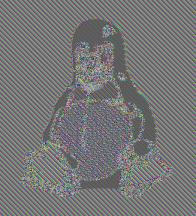
\includegraphics[width=\textwidth]{images/Tux_ecb.jpg}
		\caption{ECB-Modus}
	\end{subfigure}
	\hfill
	\begin{subfigure}[b]{.3\textwidth}
		\centering
		
\includegraphics[width=\textwidth]{images/Tux_secure.jpg}
		\caption{anderer Modus, z.B. CTR}
	\end{subfigure}
	\flushright{\scriptsize{Quelle: \url{http://en.wikipedia.org/wiki/Block_cipher_mode_of_operation}}}
	\caption{Beispielhafter Vergleich verschiedener Modi}
	\label{fig:tux_encryption_modes}
\end{figure}

%\\ {\tiny{Quelle: \url{http://en.wikipedia.org/wiki/Block_cipher_mode_of_operation}}}

Fundamentale Eigenschaften der einzelnen Modi sind in der unteren Tabelle aufgeführt. Beachte, dass die hier vorgestellten Modi nur ein Teil einer Vielzahl an existierenden Betriebsmodi sind.
\begin{table}[h]
\captionsetup{labelformat=empty}
\captionsetup{singlelinecheck=false}
\captionsetup{font=footnotesize}
\centering
	\begin{tabularx}{\textwidth}{ | X | X | X | X | X |} 
		\hline
		  & ECB & CBC & CTR & GCM \\ 
		\hline
		Hauptsächliche Verwendung & Für Nachrichten, die kürzer als ein Block sind & Für Nachrichten, die länger als ein Block sind 
		& Für Nachrichten, die länger als ein Block sind & Für Nachrichten, die länger als ein Block sind und vor Manipulationen geschützt werden müssen \\ 
		\hline
		\parbox{3cm}{IND-CPA\(^{\ast}\) } sicher & Nein & Ja\(^{\ast\ast}\) & Ja\(^{\ast\ast}\) & Ja\(^{\ast\ast}\) \\
		\hline
		 Parallelisierbar & Ja & Nur Entschlüsselung  & Ja & Ja, das Signieren selbst aber nicht \\ 
		\hline
		Bit-Fehler im Block X & Block X zerstört & Block X zerstört und 1 Bit im Block (X - 1) geändert 
		& 1 Bit verändert & 1 Bit verändert und geänderte Signatur \\
		\hline
	\end{tabularx}
	\caption{\(^{\ast}\) IND-CPA ist ein Sicherheitsbegriff und wird in \hyperref[def:ind-cpa]{Abschnitt \ref{def:ind-cpa}} definiert \\ 
		\(^{\ast\ast}\) Hierfür muss der \(IV\) vor jeder Verschlüsselung zufällig gleichverteilt gewählt werden}
\end{table}
\chapter{Kryptographische Sicherheitsbegriffe}
\section{Semantische Sicherheit}\label{ch:sicherheitsbegriffe:semantischesicherheit}
Nachdem wir uns bereits mit Verschlüsselungssystemen auseinandergesetzt haben, stellt sich natürlich die Frage, welche Form von Sicherheit wir erreichen möchten. 
Eines der primären Ziele war es bisher, dass ein Angreifer durch das Chiffrat keinerlei Informationen über den Klartext erhält. Dies entspricht dem Begriff der \emph{semantischen Sicherheit},
welcher 1983 von Goldwasser und Micali \cite{Goldwasser1984} definiert wurde und besagt konkret:
\begin{quote}
	\emph{Alles was mit $\ciphert$ (effizient) über $\plaint$ berechnet werden kann, kann auch ohne das Chiffrat berechnet werden.}
\end{quote}
Dabei ist zu beachten, dass diese Form von Sicherheit lediglich passive Angriffe abdeckt.

\begin{definition}[Semantische Sicherheit]\label{def:semsec}
Ein symmetrischer Verschlüsselungsalgorithmus ist semantisch sicher, wenn es für jede $\plaint$-Verteilung von Nachrichten gleicher Länge, jede Funktion $f$
und jeden \emph{effizienten} Algorithmus $\A$ einen \emph{effizienten} Algorithmus $\B$ gibt, so dass
\begin{align*}
	\text{Pr}\left[ \A^{\enc (\key,\cdot)} \left( \enc \left( \key, \plaint \right) \right) = f(\plaint) \right] - \text{Pr} \left[ \B (\epsilon) = f (\plaint) \right]
\end{align*}
\emph{klein} ist.
\end{definition}

Allerdings impliziert die Existenz von mehrfach benutzbaren, semantisch sicheren Verfahren damit $P \neq NP$. Das bedeutet, falls $P = NP$ gelten sollte, kann
es kein solches Verfahren geben. Außerdem ist diese Definition technisch schwer zu handhaben, da sie viele Quantoren enthält. Hierfür wurden handlichere
aber äquivalente Begriffe eingeführt wie beispielsweise \emph{IND-CPA}.

\section{Der IND-CPA-Sicherheitsbegriff}\label{def:ind-cpa}
IND-CPA steht für \emph{indistinguishability under chosen-plaintext attacks}. Bei einem Verfahren, welches diese Sicherheit besitzt, kann ein Angreifer $\A$
die Chiffrate von selbstgewählten Klartexten nicht unterscheiden. Um ein Verschlüsselungsverfahren $\enc$ auf die IND-CPA Eigenschaft zu überprüfen, führen wir folgendes Experiment, bei dem $\A$ Zugriff auf ein $\enc(\key,\cdot)$-Orakel\footnote{Ein Orakel kann man sich als \textit{black box} vorstellen, bei der der Fragende zwar das Ergebnis, jedoch nichts über dessen Berechnung in Erfahrung bringt.} hat, durch:
\begin{itemize}
\item $\A$ wählt zwei Nachrichten $\plaint_1$ und $\plaint_2$ gleicher Länge
\item $\A$ erhält $\ciphert^{*} := \enc(\key, \plaint_{b})$ für zufällig gleichverteilt gewähltes $b \in \{1, 2\}$.
\item $\A$ gewinnt, wenn er $b$ korrekt errät.
\end{itemize}
Ein Verfahren ist nun IND-CPA-sicher, wenn der Vorteil des Angreifers gegenüber dem Raten einer Lösung, also $\Pr \left[ \A \text{
gewinnt} \right] - \frac{1}{2}$, für alle Angreifer $\A$ vernachlässigbar klein ist. 
\begin{theorem}
Ein Verfahren ist genau dann semantisch sicher, wenn es IND-CPA-sicher ist.
\end{theorem}

\subsection{Beispiel ECB-Modus}
\begin{description} 
	\item[Behauptung] Keine Blockchiffre ist im ECB-Modus IND-CPA-sicher.
	\item[Beweis] Betrachte folgenden Angreifer $\A$:
	\begin{itemize}
		\item $\A$ wählt zwei Klartextblöcke $\plaint_1 \neq \plaint_2$ beliebig.
		\item $\A$ erhält  $\ciphert^{*} := \enc(\key, \plaint_{b})$ für zufällig gleichverteilt gewähltes $b \in \{1, 2\}$.
		\item $\A$ erfragt $\ciphert_1 = \enc(\key, \plaint_1)$ durch sein Orakel.
		\item $\A$ gibt 1 aus, genau dann, wenn $\ciphert_1 = \ciphert^{*}$, sonst gibt er 2 aus.
		\item $\Pr \left[ \A \text{ gewinnt} \right] = 1$, also ist das Schema nicht IND-CPA-sicher.
	\end{itemize}
\end{description}
Bei diesem Beispiel nutzt der Angreifer die Schwäche des ECB-Modus, dass gleiche Klartextblöcke immer zu gleichen Chiffrat-Blöcken werden, aus.

\subsection{Beispiel CBC-Modus}
Wie wir bereits im Abschnitt~\ref{ssec:cbc} gelernt haben, gilt bei der Verwendung des CBC-Modus: 
\begin{align*}
\ciphert_i = \enc(\key, \plaint_i \oplus \ciphert_{i-1}) \text{, mit } \ciphert_0 := IV.
\end{align*}
Im Folgenden nehmen wir an, dass der Initialisierungsvektor $IV$ bei jeder Verschlüsselung zufällig gleichverteilt gewählt wird. Somit wird verhindert, dass sich der Modus bei einem einzelnen Datenblock gleich dem ECB-Modus verhält. Im CBC-Modus existiert diese Problematik für längere Nachrichten, selbst bei festem und öffentlichem $IV$, generell nur für den ersten Datenblock, da darauffolgende Datenblöcke mit den vorausgehenden Chiffraten verkettet werden und somit kein direkter Zusammenhang mehr zwischen Daten- und Chiffratblock besteht. Allerdings werden bei der IND-CPA-Sicherheit zwei einzelne Blöcke verwendet, weshalb wir hier auf die Variante mit zufälligem $IV$ ausweichen.

Das zufällige Wählen eines $IV$ löst zwar ein Problem, erzeugt jedoch ein anderes: Um eine korrekte Entschlüsselung zu gewährleisten, muss der gewählte $IV$ mitgesendet werden. Das resultierende Problem ist nun, dass ein Angreifer eben diesen $IV$ verändern kann und somit beliebige Manipulationen am ersten Block einer bekannten Nachricht vornehmen kann.

\begin{description} 
	\item[Behauptung] Eine Blockchiffre ist im CBC-Modus genau dann IND-CPA-sicher, wenn die Verschlüsselungsfunktion $\enc(\key,\cdot): \{0,1\}^l \rightarrow
	\{0,1\}^l$ nicht von einer Zufallsfunktion $R: \{0,1\}^l \rightarrow \{0,1\}^l$ unterscheidbar ist.
	\item[Beweisidee]~
	\begin{description}
		\item[IND-CPA-sicher $\Rightarrow$ Ununterscheidbarkeit]~\\
		$\Leftrightarrow$ IND-CPA-unsicher $\Leftarrow$ Unterscheidbarkeit~\\
		Wenn ein Angreifer $\enc(\key, \cdot)$ von einer Zufallsfolge unterscheiden kann, ist zwischen mindestens zwei Verschlüsselungsergebnissen ein Zusammenhang erkennbar. Es gibt somit mindestens einen Fall, bei dem der Angreifer zusätzliche Informationen für das Zuordnen des Chiffrats besitzt. Daher gilt für zufällig gewählte Nachrichten im IND-CPA-Experiment: Pr$[\A$ gewinnt$] > \frac{1}{2} \Rightarrow$ IND-CPA-unsicher.
		\item[IND-CPA-sicher $\Leftarrow$ Ununterscheidbarkeit]~\\
		Wenn die Verschlüsselungsfunktion aus Sicht des Angreifers nicht von einer Zufallsfunktion unterscheidbar ist, gibt es keine bekannten Zusammenhänge der Verschlüsselungen. Somit ist die Wahrscheinlichkeit, dass der Angreifer ein Chiffrat korrekt zuordnet, genau $\frac{1}{2}$.
	\end{description}
\end{description}

\section{Der IND-CCA-Sicherheitsbegriff}
Der CPA-Angreifer ist mit Zugriff auf ein Verschlüsselungsorakel ausgestattet. Er kann sich jedmöglichen Klartext verschlüsseln lassen und
versuchen, Muster in den Ausgaben des Orakels zu erkennen. Eingeschränkt ist er dennoch, da ihm die Möglichkeit fehlt, zu beliebigen
Ciphertexten den Klartext zu berechnen. Ein stärkerer Sicherheitsbegriff ist daher IND-CCA. Ähnlich wie IND-CPA, steht IND-CCA abkürzend für \emph{indistinguishability under chosen-ciphertext attacks}. Dabei suggeriert das Akronym CCA bereits einen mächtigeren Angreifer. Das in \ref{def:ind-cpa} vorgestellte Experiment können wir problemlos auf einen IND-CCA-Angreifer anpassen. Modifiziert ergibt sich:

\begin{itemize}
	\item Der Angreifer $\A$ besitzt Zugriff auf ein $\enc(\key,\cdot)$-Orakel und ein $\dec(\key,\cdot)$-Orakel
	\item $\A$ wählt zwei Nachrichten $\plaint_1$ und $\plaint_2$ gleicher Länge
	\item $\A$ erhält $\ciphert^{*} := \enc(\key, \plaint_{b})$  für ein zufällig gleichverteilt gewähltes $b \in \{1, 2\}$.
	\item $\A$ gewinnt, wenn er $b$ korrekt errät.
\end{itemize} 

Natürlich darf der Angreifer den Klartext zum Chiffrat $\ciphert^{*}$ nicht bei dem Entschlüsselungsorakel erfragen. Ein Angriff wäre ansonsten trivial und es gäbe kein Verfahren, dass dem IND-CCA-Sicherheitsbegriff genügt. 

%Wieso braucht man hier das hardcoded Leerzeichen und oben nicht?%
Analog heißt ein Verfahren nun IND-CCA-sicher, wenn der Vorteil des Angreifers gegenüber dem Raten einer Lösung, also $\text{Pr} \left[ \A\ \text{gewinnt} \right] - \frac{1}{2}$, für alle Angreifer vernachlässigbar klein ist.

Etwas granularer kann bei IND-CCA zwischen einer adaptiven und einer nichtadaptiven Variante unterschieden werden. Erstere erlaubt dem Angreifer weitere Berechnungen, auch nachdem $\ciphert^{*}$ bereits erhalten wurde, wohingegen die nichtadaptive Variante solche Berechnungen explizit verbietet. In der Theorie kann sich ein adaptiver Angreifer also auch von $\ciphert^{*}$ abhängige Ciphertexte entschlüsseln lassen. Sprechen wir in diesem Skript von IND-CCA, so gehen wir von der adaptiven Variante aus.

\section{Sicherheitsparameter und effiziente Angreifer}\label{sec:secparam}
Zu einer Funktion, für die sicherheitsrelevante Eigenschaften gefordert werden, wird in der Kryptographie oft ein \emph{Sicherheitsparameter} $k$ definiert. Informell gesagt, legt $k$ das Sicherheitsniveau der Funktion fest. Beispielsweise parametrisiert er den Bildbereich einer \hyperref[cha:hash]{Hashfunktion}, wo ein größerer Bildbereich bei gleichem Urbildbereich zu einer geringeren Kollisionswahrscheinlichkeit führt.
\begin{beispiel}
	Um die Intuition rechnerisch zu belegen, definieren wir eine Funktion
	\begin{align*}
		H : \{0, 1\}^{1024} \rArrow \{0, 1\}^{k}\, ,
	\end{align*}
	wobei, falls $k = 512$,
	\begin{align*}
		\Pr \left[ \exists x' \neq x : H(x') = H(x) \mid x \stackrel{\textdollar}{\longleftarrow} \{0, 1\}^{1024} \right] > \frac{1}{2}
	\end{align*}
	und falls $k = 256$,
	\begin{align*}
		\Pr \left[ \exists x' \neq x : H(x') = H(x) \mid x \stackrel{\textdollar}{\longleftarrow} \{0, 1\}^{1024} \right] > \frac{3}{4}
	\end{align*}
\end{beispiel}
Ein weiteres Beispiel für die Anwendung des Sicherheitsparameters findet sich bei symmetrischen Verschlüsselungsverfahren, bei welchen die durch $k$ festgelegte Länge des Schlüssels den Aufwand einer Brute-Force-Attacke bestimmt. Dabei wird $k$ vor der Schlüsselerzeugung ausgehandelt und es kann davon ausgegangen werden, dass eine ehrliche Partei sich an die Abmachung hält.
Die Sicherheit des Verfahrens darf allerdings nicht von der Geheimhaltung des Sicherheitsparameters abhängen. 

Zur Analyse der Sicherheitseigenschaften eines kryptographischen Verfahrens betrachtet man üblicherweise einen Angreifer, der \emph{effizient}, das heißt in seiner Rechenzeit eingeschränkt ist. Intuitiv wird in der Komplexitätstheorie ein effizienter Algorithmus mit einer polynomial-beschränkten Laufzeit in der Eingabegröße gleichgesetzt. 
In anderen Worten ist ein Algorithmus bei Eingabe eines Bit-Strings der Länge $n$ genau dann effizient, wenn seine Laufzeit im schlechtesten Fall in $O(n)$ liegt.
Um mit dieser Idee konsistent zu bleiben, wird in der Kryptographie einem Angreifer auf ein Verfahren ein Bit-String $1^k$ von $k$ Einsen übergeben, um die Rechenzeit durch den zugrundeliegenden Sicherheitsparameter zu begrenzen. 
Ein effizienter Angreifer muss also in $O(k)$-Schritten eine Lösung berechnen. Somit ist beispielsweise die eingangs erwähnte Brute-Force-Attacke auf einen Schlüsselraum $\{0, 1\}^{k}$ ausgeschlossen, da die Laufzeit in $O(2^{k})$ liegt, also exponentiell ist.
Neben der Begrenzung der Rechenzeit erlauben wir einem Angreifer, um ein realistisches Szenario abzubilden, zu jedem Zeitpunkt eine \emph{faire} Münze zu werfen, das heißt, eine Lösung zu raten. Einen solchen Angreifer bezeichnen wir als \emph{probabilistic polynomial time} (PPT) Angreifer.
%Was ist mit den Längen der anderen Eingaben, die ein Angreifer bekommt?

Damit ein Verschlüsselungsverfahren grundsätzlich als sicher angenommen werden kann, muss die Erfolgswahrscheinlichkeit eines Angreifers möglichst klein sein und darf idealerweise nur vom Zufall abhängen.
Da der Sicherheitsparameter für jedes Verfahren beliebig variiert werden kann, erscheint es intuitiv logisch, die Sicherheit nicht in Abhängigkeit der Größe von $k$ zu definieren. Vielmehr fordern wir für eine bestimmte Sicherheitseigenschaft, dass ein PPT Angreifer die Charakteristik nur mit \emph{vernachlässigbarer} Wahrscheinlichkeit in $k$ brechen kann.
\begin{definition}[Vernachlässigbarkeit]
	Es sei $f$ eine Funktion, $k$ eine Konstante und $p(\cdot)$ ein beliebiges Polynom. Dann heißt $f$ vernachlässigbar in $k$, wenn
	\begin{align*}
		\exists k_0 : \forall k \geq k_0 : \vert f(k) \vert \leq \frac{1}{p(k)} 
	\end{align*}
\end{definition}
Beispielsweise ist $f = \frac{1}{2^k}$ vernachlässigbar in $k$, $f = \frac{1}{k^2}$ jedoch nicht.

Dass ein Verfahren in der Praxis bei zu klein gewähltem Sicherheitsparameter, trotz vernachlässigbarer Erfolgswahrscheinlichkeit eines PPT Angreifers, keine Sicherheit bieten kann, ist trivial.
\chapter{Hashfunktionen}\label{cha:hash}
\section{Grundlagen}
Hashfunktionen sind Funktionen, die von einer großen, potentiell unbeschränkten Menge in eine kleinere Menge abbilden, also
\begin{align*}
H_k\colon \{0,1\}^* \rightarrow \{0,1\}^k\, ,
\end{align*}
wobei $k$ den in \ref{sec:secparam} eingeführten Sicherheitsparameter bezeichnet.
Diese Funktionen werden dazu verwendet, größere Datenmengen effizient zu kennzeichnen (ihnen sozusagen einen Fingerabdruck zuzuordnen). Die Anwendungsgebiete für Hashfunktionen in der Informatik sind vielfältig, wir werden uns aber in diesem Skript auf ihre kryptographischen Anwendungen beschränken.

\section{Sicherheitseigenschaften}
Um eine Hashfunktion im kryptographischen Sinne verwenden zu können, reicht eine Funktion, die von einer großen Menge in eine kleine Menge abbildet, nicht aus.
Sie muss zusätzlich einige weitere Anforderungen erfüllen.

\subsection{Kollisionsresistenz}
Die wichtigste Eigenschaft einer Hashfunktion $H$ ist die Kollisionsresistenz (\textit{collision resistance}). Das bedeutet, es soll schwierig sein, zwei
unterschiedliche Urbilder $X, X'$ zu finden, für die gilt: 
\begin{align*}
X \neq X' \text{ und } H(X) = H(X')
\end{align*}

Da wir von einer großen in eine kleine Menge abbilden, kann $H$ nicht injektiv sein. Es ist uns also nicht möglich, Kollisionen komplett zu
verhindern. Trotzdem können wir fordern, dass diese möglichst selten auftreten. Präziser formuliert verlangen wir, dass bei jeder
kollisionsresistenten Hashfunktion ein PPT Algorithmus eine Kollision
nur mit im Sicherheitsparameter $k$ vernachlässigbarer Wahrscheinlichkeit findet.
\begin{definition}[Kollisionsresistenz]
Eine Funktion $H_k$ ist kollisionsresistent, wenn jeder PPT-Algorithmus
nur mit höchstens in $k$ vernachlässigbarer Wahrscheinlichkeit eine Kollision findet.
Präziser formuliert ist der Vorteil für jeden PPT-Angreifer $\A$
\begin{align*}
Adv^{cr}_{H,\A}(k):= \Pr \left[ (X, X') \leftarrow \A(1^k) : X \neq X' \land H_k(X) = H_k(X')\right]
\end{align*}
in $k$ vernachlässigbar.
\end{definition}

\subsection{Einwegeigenschaft}
Die zweite kryptographisch wichtige Eigenschaft von Hashfunktionen ist die Einwegeigenschaft (\textit{pre-image resistance}), die sicherstellt,
dass eine Hashfunktion nur in eine Richtung berechenbar ist. Genauer gesagt fordern wir, dass es bei einem gegebenen Wert $H(X)$ \emph{schwierig} ist, ein
passendes $X$ zu finden.

Es stellt sich nun die Frage, wie eine Hashfunktion beschaffen sein muss, damit sie die Einwegeigenschaft erfüllen kann. Ist z.B. die Urbildmenge zu klein, kann
durch Raten einfach auf ein passendes $X'$ geschlossen werden. Außerdem sollte es intuitiv keinen Kandidaten $X'$ als Urbild für $H(X)$ geben, der
wahrscheinlicher ist als andere Kandidaten. Um das zu erreichen, wird für die Elemente der Urbildmenge üblicherweise eine Gleichverteilung angestrebt.
\vspace{10pt}

\begin{definition}[Einwegfunktion]
Eine über $k$ parametrisierte Funktion $H$ ist eine Einwegfunktion bezüglich der Urbildverteilung $\chi_k$, wenn jeder PPT-Algorithmus nur mit höchstens
in $k$ vernachlässigbarer Wahrscheinlichkeit ein Urbild eines gegebenen, aus $\chi_k$ bezogenen Bildes findet. Genauer ist der Vorteil für jeden PPT-Angreifer $\A$
\begin{equation*}
Adv^{ow}_{H,\A}(k):= \Pr \left[ X' \leftarrow \A(H(X), 1^k) : H(X) = H(X')\right]
\end{equation*} 
in $k$ vernachlässigbar, wobei $X \leftarrow \chi_k$ gewählt wurde. Dabei muss $\A$ nicht zwingend $X' = X$ zurückgeben.
\end{definition}

~\\
Die Forderungen nach Kollisionsresistenz und Einwegeigenschaft, die wir bisher für eine kryptographische Hashfunktion aufgestellt haben, hängen bei näherer
Betrachtung sehr eng miteinander zusammen. Das führt uns zu folgender Feststellung:
\vspace{10pt}

\begin{theorem}
Jede kollisionsresistente Hashfunktion $H_k \colon \{0,1\}^* \rightarrow \{0,1\}^k$ ist eine Einwegfunktion bzgl. der Gleichverteilung auf $\{0,1\}^{2k}$.
\end{theorem}

\begin{beweisidee}
$H_k$ hat $2^k$ Bilder und $2^{2k}$ Urbilder. Es gibt also weniger als
$2^k$ Nachrichten, die auf einen Hashwert abgebildet werden, der genau einer
Nachricht zugeordnet werden kann. Es hat also bei $X \in \{0,1\}^{2k}$ fast jedes
Urbild $X$ viele "`Nachbarn"' $X'$ mit $H(X) = H(X')$, denn für die
Wahrscheinlichkeit, dass ein Element $H(X)$ der Bildmenge nur ein
einziges Urbild $X$ besitzt, gilt

\begin{equation*}
\Pr \left[ | H^{-1}(H(X))| = 1\right] \leq \frac{2^k}{2^{2k}} = \frac{1}{2^k}.
\end{equation*}
Die Wahrscheinlichkeit ist also vernachlässigbar im Sicherheitsparameter
$k$.
\end{beweisidee}

\begin{beweis}
Zu jedem $H$-Invertierer $\A$ geben wir nun einen $H$-Kollisionsfinder $\B$ an mit
\begin{equation*}
Adv^{cr}_{H,\B}(k) \geq \frac{1}{2} \cdot Adv^{ow}_{H,\A}(k) - \frac{1}{2^{k+1}}
\end{equation*} 
Nun wählt $\B$ ein $X \leftarrow \{0,1\}^{2k}$ gleichverteilt zufällig und gibt $H(X)$ als Eingabe an $\A$. $\B$ setzt nun $X' \leftarrow \A(1^k, H(X))$ und
gibt $(X, X')$ aus.\\
Dann gilt für $\B$s Erfolgswahrscheinlichkeit:
\begin{align*}
	&\Pr \left[\B \text{ gewinnt}\right]\\
	&= \Pr\left[H(X) = H(X') \land X \not = X'\right]\\
	&= \Pr \left[\A \text{ invertiert} \land X \not = X'\right]\\
	&\geq \Pr \left[\A \text{ invertiert} \land X \not = X' \land \vert H^{-1}(H(X)) \vert > 1\right]\\
	&= \underbrace{\Pr \left[X \not = X' \biggm| \A \text{ invertiert} \land \vert H^{-1}(H(X)) \vert > 1\right]}_{\geq \frac{1}{2}}
	\cdot \underbrace{\Pr \left[\A \text{ invertiert} \land \vert H^{-1}(H(X)) \vert > 1\right]}_{\geq \Pr \left[\A \text{ invertiert}\right] - \frac{1}{2^k}}\\
	&\geq \frac{1}{2} \cdot Adv^{ow}_{H,\A}(k) - \frac{1}{2^{k+1}}
\end{align*}
\qed
\end{beweis}


\subsection{Target Collision Resistance}
Die \textit{Target Collision Resistance} (auch \textit{second pre-image resistance} oder \textit{universal one-way}) ist eine weitere Eigenschaft, die zur
Bewertung von Hashfunktionen herangezogen wird. Genügt eine Hashfunktion $H$ der Target Collision Resistance, ist es \textit{schwierig}, für ein gegebenes
Urbild $X$ ein $X' \not = X$ zu finden, für das gilt: $H(X') = H(X)$.

Die Target Collision Resistance stellt einen Zwischenschritt zwischen Kollisionsresistenz und Einwegeigenschaft dar: Kollisionsresistenz impliziert die
Target Collision Resistance, welche wiederum die Einwegeigenschaft impliziert. Formal ergibt sich:\\

\begin{definition}[Target Collision Resistance]
Eine über $k$ parametrisierte Funktion $H$ genügt der Target Collision Resistance, falls für jeden PPT-Angreifer $\A$ bei gegebenem, zufällig gezogenem $X$ die Wahrscheinlichkeit
\begin{equation*}
Adv^{tcr}_{H,\A}(k):= \Pr \left[ X' \leftarrow \A(X, 1^k) : X \neq X' \land H_k(X) = H_k(X')\right]
\end{equation*}
in $k$ vernachlxässigbar ist.
\end{definition}
\subsection{Beispiele}

\begin{beispiel}[Kollisionsresistenz bei Signaturverfahren]
Eve und Bob beschließen, gemeinsam online Verträge abzuschließen. Hierzu
verwenden sie ein \textit{Hash-then-Sign}-Verfahren, dass in Kapitel
\ref{subsec:hash-then-sign} noch näher betrachtet wird. Wir können uns
das Verfahren wie 
folgt vorstellen: 
\begin{enumerate}
\item Eve sendet eine Nachricht an Bob.
\item Bob berechnet den Hashwert und erstellt kryptographische
  Signatur (eine Art \glqq elektronische Unterschrift\grqq, siehe
  Kapitel \ref{cha:symauth}) für diesen Hashwert.
\item Bob sendet diese Signatur an Eve
\item Eve berechnet eine eigene Signatur für die Nachricht. Nun kann Eve
  anderen gegenüber beweisen, dass sie und Bob dem Inhalt der Nachricht
  zustimmen. 
\end{enumerate}
Ist die Hashfunktion nun nicht kollistionsresistent, ist folgender
Angriff möglich:
\begin{enumerate}
\item Eve erstellt zwei Verträge $\plaint_1$ und $\plaint_2$ mit
  $H(\plaint_1) = H(\plaint_2)$, wobei
  $\plaint_1$ ein fairer Vertrag und $\plaint_2$ ein unfairer Vertrag
  ist, dem Bob niemals zustimmen würde.
\item Eve sendet $\plaint_1$ an Bob. Bob stimmt dem Vertrag zu und
  sendet Eve deshalb seine Signatur für $H(\plaint_1)$.
\item Eve benutzt diese Signatur, um gegenüber anderen vorzuweisen, dass
  Bob dem Vertrag $\plaint_2$ zugestimmt hat.
\end{enumerate}
\end{beispiel}

\begin{beispiel}[Einweg-Eigenschaft beim Speichern von Passwörtern]
Angewendet werden Hashes beispielsweise beim Speichern von
Passwörtern auf einem Server. Der Server speichert nur $H(X)$ ab und
vergleicht bei einem Anmeldungsversuch lediglich $H(X)$ mit dem ihm vom
Client zugesendeten $H(X')$. Dadurch muss das Passwort nicht im Klartext
auf dem Server liegen. Wie wir in Kapitel~\ref{cha11} sehen werden, gibt
es aber effiziente Angriffsmöglichkeiten, weswegen heutzutage neben dem
Hash des Passworts auch noch ein \emph{Salt} gespeichert wird, der
zufällig für jedes Passwort generiert wird.
Die Einwegeigenschaft der Hashfunktion stellt sicher, dass ein
Angreifer, der in Besitz der Liste der Passtwort-Hashes kommt, aus
diesen keine Passwörter berechnen kann.
\end{beispiel}

\begin{beispiel}[Target-Kollisionsresistenz in der Computer-Forensik]
Eine Anwendung von kryptographischen Hashfunktionen ist die
Computer-Forensik. Hierbei wird, z.B. zur Verbrechensermittlung, eine
Festplatte auf bestimmte Dateien hin untersucht. Da man sich den Aufwand
ersparen möchte, alle Dateien händisch zu untersuchen, geht man wie
folgt vor:
\begin{enumerate}
  \item Erstelle eine Whitelist, die für bekannte, gutartige
    Dateien(z.B. Bestandteile des Betriebssystems) die Hashwerte
    enthält, sowie ein Blacklist für entsprechend bösartige Dateien.
  \item Untersuche diejenigen Dateien, die auf keiner der beiden Listen
    genannt sind, genauer.
\end{enumerate}

Wenn die verwendete Hash-Funktion nun nicht target-kollisionsresistent
ist, kann dies verwendet werden, um bösartige Dateien zu
verstecken. Angenommen, ein Terrorist möchte die Datei
\texttt{bombenbauanleitung.pdf} so speichern, dass sie im Falle einer
Beschlagnamung des Computers nicht entdeckt wird. Er benennt sie deshalb
um in \texttt{betriebsanleitung.pdf}. Außerdem bricht er die
Target-Kollisionsresistenz und verändert seine Datei so, dass ihr Hash
mit dem der Betriebsanleitung des Betriebssystems übereinstimmt. Diese
wird mit großer Wahrscheinlichkeit auf der Whitelist der Polizei
stehen. Deshalb wird sie bei einer Untersuchung nicht
auffallen\cite{Stevens2012}.
\end{beispiel}
\section{Merkle-Damgård-Transformation}
\label{ch:hash:merkledamgard}
In der Praxis werden Hashfunktionen benötigt, die nicht nur die Eigenschaften aus den obigen Abschnitten berücksichtigen, sondern auch flexibel in ihrer
Eingabelänge und konstant in ihrer Ausgabelänge sind. Typischerweise werden für diesen Zweck \emph{Merkle-Damgård-Transformation} eingesetzt. 

\subsection{Struktur von Merkle-Damgård}
Die Eingabenachricht wird bei einer Merkle-Damgård-Transformation $H_{\textnormal{MD}}$ zunächst in Blöcke $\plaint_{1},\dots, \plaint_{n}$ mit fester Blocklänge $l$ aufgeteilt.
Auf diese Blöcke wird anschließend nacheinander eine Kompressionsfunktion $F \colon \{0, 1\}^{l + k} \rightarrow \{0,1\}^{k}$ angewendet, die %die Blöcke mithilfe eines Eingabeparameters $Z$ auf eine festgelegte Länge
die Blöcke auf eine feste Länge $k \leq l$ verkürzt.

Aus dem ersten Nachrichtenblock $\plaint_{1}$ und dem Initialisierungsvektor $IV \in \{0, 1\}^k$  wird durch die Kompressionsfunktion ein Bitstrom $Z_1$ der Länge $k$
berechnet, der mit Hilfe von $\plaint_2$ zu $Z_2$ berechnet wird. Diese Berechnung setzen wir analog für die restlichen Nachrichtenblöcke fort und erhalten mit $Z_{n}$ den Hashwert für die Nachricht. Formal dargestellt erhalten wir:
\begin{align*}
	Z_0 &= IV\\
	\forall i \in \{1,\dots, n\}\colon Z_{i} &= F(Z_{i-1} \concat X_{i})
\end{align*}
Der Ablauf ist schematisch in Abbildung~\ref{fig:md-konstruktion} gezeigt.

Der Initialisierungsvektor IV wird dabei für jede Hashfunktion fest gewählt. Aus Sicherheitsgründen ist es, wie wir in Beweis~\ref{md-proof} sehen werden, notwendig, die Nachrichtenlänge an das Ende der Nachricht anzuhängen. Falls es im letzten Block nicht genügend freie Bits gibt, wird diese an das Ende eines neuen Blocks geschrieben. Die übrigen Bits werden gepaddet.

%Ist der letzte Block $M_{n}$ zu kurz, wird er auf die benötigte Blocklänge gepaddet. 
%Das Padding enthält dabei die Nachrichtenlänge, um zu verhindern, dass Verlängerungen der Nachricht für einen Angriff genutzt werden können.
\begin{figure}[h]
\begin{center}
\unitlength=1mm
\linethickness{0.4pt}
\begin{picture}(110,20)

\put(5,5){\vector(1,0){15}}
\put(12,6){\makebox(0,0)[cb]{IV}}

\put(25,15){\vector(0,-1){7.5}}
\put(28,10){\makebox(0,0)[cb]{$M_1$}}

\put(20,2.5){\framebox(10,5){$F$}}

\put(30,5){\vector(1,0){12}}
\put(36,6){\makebox(0,0)[cb]{$Z_1$}}

\put(47,15){\vector(0,-1){7.5}}
\put(50,10){\makebox(0,0)[cb]{$M_1$}}

\put(42,2.5){\framebox(10,5){$F$}}

\put(52,5){\vector(1,0){12}}
\put(58,6){\makebox(0,0)[cb]{$Z_2$}}

\put(68,4){\makebox(0,0)[cb]{\ldots}}

\put(72,5){\vector(1,0){12}}
\put(78,6){\makebox(0,0)[cb]{$Z_{n-1}$}}

\put(84,2.5){\framebox(10,5){$F$}}

\put(89,15){\vector(0,-1){7.5}}
\put(92,10){\makebox(0,0)[cb]{$M_{n}$}}

\put(94,5){\vector(1,0){12}}
\put(100,6){\makebox(0,0)[cb]{$Z_{n}$}}

\end{picture}
\end{center}
\caption{Merkle-Damgård-Transformation $H_{\textnormal{MD}}$}
\label{fig:md-konstruktion}
\end{figure}

\subsection{Sicherheitseigenschaften der Merkle-Damgård-Transformation}
Die Sicherheit einer Merkle-Damgård-Transformation $H_{\textnormal{MD}}$ hängt stark von der verwendeten Kompressionsfunktion $F$ ab:
\begin{theorem}
Ist $F$ kollisionsresistent, so ist auch $H_{\textnormal{MD}}$ kollisionsresistent.
\end{theorem}

\begin{beweis}\label{md-proof}
Gegeben sei zwei Nachrichten $M \neq M'$ mit $H_{\textnormal{MD}}(M) = H_{\textnormal{MD}}(M')$. Wir führen diese Kollision nun auf eine Kollision in $F$ zurück. 
Da es eine Kollision in $H_{\textnormal{MD}}$ gibt, gilt $Z_{n} = F(Z_{n-1} \concat M_{n}) = F(Z'_{n-1} \concat M'_{n}) = Z'_{n}$.
\begin{description}
	\item[Fall 1:] $Z_{n-1} \neq Z'_{n-1}$ oder $M_{n} \neq M'_{n}$ $\Rightarrow$ Es wurde eine Kollision in $F$ gefunden. 
	\item[Fall 2:] $Z_{n-1} = F(Z_{n-2} \concat M_{n-1}) = F(Z'_{n-2} \concat M'_{n-1}) = Z'_{n-1}$ $\Rightarrow$ Wir überprüfen analog beide Fälle für die Bitstrings $Z_{n-2} \concat M_{n-1}$ und $Z'_{n-2} \concat M'_{n-1}$.
\end{description}
Wir überprüfen beide Fälle für alle Argumente $Z_{i-1} \concat M_{i}$, $Z'_{i-1} \concat M'_{i}$ $(1 \leq i \leq n)$, bis wir eine Kollision in $F$ gefunden haben. Da nach Voraussetzung $M \neq M'$ gilt und die Nachrichtenlängen angehängt wurden, gibt es mindestens ein $M_{i} \neq M'_{i}$ und damit eine Kollision in $F$.
Hätten wir also einen Angreifer, der effizient Kollisionen für $H_\textnormal{MD}$
findet, könnten wir daraus einen Angreifer konstruieren, der effizient
Kollisionen für $F$ berechnen, was im Widerspruch zur angenommenen
Kollisionsresistenz von $F$ steht.
\qed
\end{beweis}

\subsection{Bedeutung von Merkle-Damgård}
\subsubsection{Secure Hash Algorithm (SHA)}
Im Jahr 1995 veröffentlichte die NIST den von der NSA entworfenen, auf der Merkle-Damgård-Transformation beruhenden, kryptographischen Hashalgorithmus \emph{Secure Hash Algorithm 1} (SHA-1) \cite{NIST_SHA95}. Lange Zeit war SHA-1 die wichtigste kryptographische Hashfunktion, bis der Algorithmus im Jahr 2005 zumindest theoretisch gebrochen wurde. Es existieren also Angriffe, die schneller als eine Brute-Force-Suche sind, eine explizite Kollision wurde bislang allerdings nicht gefunden. In Folge des Bekanntwerdens der Schwachstellen empfiehlt die NIST auf die Verwendung von SHA-1 zu verzichten. Dennoch hat SHA-1 wenig von seiner Verbreitung eingebüßt und wird heutzutage immer noch weitreichend verwendet, z.B. bei Prüfsummen.

\paragraph*{Ablauf des Hash-Vorgangs}

\begin{enumerate}
	\item Teile die Nachricht in $n$ 512-Bit große Blöcke $\plaint_{1},\dots,\plaint_{n}$ auf und padde den letzten Block bei Bedarf.
	\item Initialisiere $H_0^{(0)}, \dots, H_4^{(0)}$ mit fest gewählten Konstanten und setze $a = H_0^{(0)}, \dots, e = H_4^{(0)}$.
	\item Für alle Nachrichtenblöcke $\plaint_{i}$ von $i = 1,\dots,n$:
	\begin{enumerate}
		\item Führe 80 Berechnungsrunden $t = 0,\dots,79$ aus, um die neuen Hashwerte für $a,\dots,e$ zu bestimmen.	
		\begin{figure}[h]
			\centering
			\tikzstyle{every circle node}= [draw]
			\begin{tikzpicture}
			\begin{scope}[>=latex] %for filled arrow tips
			\newcommand{\n}{5}
			
			\pgfmathsetmacro\minBoxWidth{(2.0)} // 2.2 old
			\pgfmathsetmacro\minBoxHeight{(0.6)} // 0.5 old
			
			\pgfmathsetmacro\xA{int(0)}
			\pgfmathsetmacro\xB{(\minBoxWidth * 1)}
			\pgfmathsetmacro\xC{(\minBoxWidth * 2)}
			\pgfmathsetmacro\xD{(\minBoxWidth * 3)}
			\pgfmathsetmacro\xE{(\minBoxWidth * 4)}
			
			\node (h0) at (\xA, {(\n -1)*2 + 2}) [draw,thick,minimum width=\minBoxWidth cm, minimum height=\minBoxHeight cm] {$H_0^{(i-1)}$};
			\node (h1) at (\xB, {(\n -1)*2 + 2}) [draw,thick,minimum width=\minBoxWidth cm, minimum height=\minBoxHeight cm] {$H_1^{(i-1)}$};
			\node (h2) at (\xC, {(\n -1)*2 + 2}) [draw,thick,minimum width=\minBoxWidth cm, minimum height=\minBoxHeight cm] {$H_2^{(i-1)}$};
			\node (h3) at (\xD, {(\n -1)*2 + 2}) [draw,thick,minimum width=\minBoxWidth cm, minimum height=\minBoxHeight cm] {$H_3^{(i-1)}$};
			\node (h4) at (\xE, {(\n -1)*2 + 2}) [draw,thick,minimum width=\minBoxWidth cm, minimum height=\minBoxHeight cm] {$H_4^{(i-1)}$};
			
			\pgfmathsetmacro\abcdeLineYCoord{(\n -1)*2 + 0.9}
			
			\node (a) at (\xA, \abcdeLineYCoord) [draw,thick,minimum width=\minBoxWidth cm, minimum height=\minBoxHeight cm] {$a$};
			\node (b) at (\xB, \abcdeLineYCoord) [draw,thick,minimum width=\minBoxWidth cm, minimum height=\minBoxHeight cm] {$b$};
			\node (c) at (\xC, \abcdeLineYCoord) [draw,thick,minimum width=\minBoxWidth cm, minimum height=\minBoxHeight cm] {$c$};
			\node (d) at (\xD, \abcdeLineYCoord) [draw,thick,minimum width=\minBoxWidth cm, minimum height=\minBoxHeight cm] {$d$};
			\node (e) at (\xE, \abcdeLineYCoord) [draw,thick,minimum width=\minBoxWidth cm, minimum height=\minBoxHeight cm] {$e$};
			
			\draw[->,semithick] (h0) -- (a);
			\draw[->,semithick] (h1) -- (b);
			\draw[->,semithick] (h2) -- (c);
			\draw[->,semithick] (h3) -- (d);
			\draw[->,semithick] (h4) -- (e);
			
			\pgfmathsetmacro\numAddBoxes{int(4)}
			\pgfmathsetmacro\lastAddBoxIndex{int(\numAddBoxes)}
			\pgfmathsetmacro\firstAddBoxYCoord{\abcdeLineYCoord - 1.5}
			
			%\node (plus0)[circle, draw] at (\xE,\firstAddBoxYCoord) {$+$};
			
			\foreach \nr in {1, ..., \numAddBoxes}{
				\node (plus\nr)[circle] at (\xE,{\abcdeLineYCoord - (1.5 * \nr)}) {$+$};
			}	
			
			\pgfmathsetmacro\lastAddBoxYCoord{\abcdeLineYCoord - 1.5 * \numAddBoxes}
			\draw[->,semithick] (e) -- (plus1);
			
			\foreach \nr in {1, ..., 3}{
				\pgfmathsetmacro\cnr{int(\nr + 1)}
				\draw[->,semithick] (plus\nr) -- (plus\cnr);
			}
			
			%draw Key and Message arrow
			\node (KeyArrow) at (\xE + 2.0, {\abcdeLineYCoord - (1.5 * 2)}) {$K_t$};
			\draw[->, semithick] (KeyArrow) -- (plus2);
			
			\node (MessageArrow) at (\xE + 2.0, {\abcdeLineYCoord - (1.5 * 4)}) {$W_t$};
			\draw[->, semithick] (MessageArrow) -- (plus4);
			
			\node (shiftL5)[ellipse, draw] at (\minBoxWidth * 0.5 + 0.1, \firstAddBoxYCoord) {$<< 5$};
			
			\node (p1)[circle, fill, inner sep=0cm, minimum size=0.12cm] at (\xA, \firstAddBoxYCoord) {};
			\draw[->, semithick] (p1) -- (shiftL5);
			\draw[->, semithick] (shiftL5) -- (plus1);
			
			\node (shiftR2)[ellipse, draw] at (\xB, \lastAddBoxYCoord) {$>> 2$};
			\draw[->, semithick] (b) -- (shiftR2);
			
			\node (rectF)[draw,thick,rounded corners,minimum width=0.6cm, minimum height=2.1cm] at (\xD + 0.7, {\abcdeLineYCoord - (1.5 * 3)}) {$F_{t}$};
			\node (p2)[circle, fill, inner sep=0cm, minimum size=0.12cm] at (\xC, {\abcdeLineYCoord - (1.5 * 3)}) {};
			\draw[->, semithick] (p2) |- (rectF);
			\draw[->, semithick] (rectF) -- (plus3);
			
			\node (p3)[circle, fill, inner sep=0cm, minimum size=0.12cm] at (\xB, {\abcdeLineYCoord - (1.5 * 3) + 0.5}) {};
			\draw[->, semithick] (p3) -- ($(rectF) + (-0.3, 0.5)$);
			
			\node (p4)[circle, fill, inner sep=0cm, minimum size=0.12cm] at (\xD, {\abcdeLineYCoord - (1.5 * 3) - 0.5}) {};
			\draw[->, semithick] (p4) -- ($(rectF) + (-0.3, -0.5)$);
			
			
			\node (aNew) at (\xA, {\lastAddBoxYCoord - 2.5}) [draw,thick,minimum width=\minBoxWidth cm, minimum height=\minBoxHeight cm] {$a$};
			\node (bNew) at (\xB, {\lastAddBoxYCoord - 2.5}) [draw,thick,minimum width=\minBoxWidth cm, minimum height=\minBoxHeight cm] {$b$};
			\node (cNew) at (\xC, {\lastAddBoxYCoord - 2.5}) [draw,thick,minimum width=\minBoxWidth cm, minimum height=\minBoxHeight cm] {$c$};
			\node (dNew) at (\xD, {\lastAddBoxYCoord - 2.5}) [draw,thick,minimum width=\minBoxWidth cm, minimum height=\minBoxHeight cm] {$d$};
			\node (eNew) at (\xE, {\lastAddBoxYCoord - 2.5}) [draw,thick,minimum width=\minBoxWidth cm, minimum height=\minBoxHeight cm] {$e$};
			%\draw[->, semithick] (shiftL5) -- (plus1);
			
			\draw[->, semithick] (a) -- (\xA, {\lastAddBoxYCoord - 1.0}) 
			-- (\xB, {\lastAddBoxYCoord - 1.5}) -- (bNew);
			
			\draw[->, semithick] (shiftR2) -- ($(shiftR2) + (0, -1)$) 
			-- (\xC, {\lastAddBoxYCoord - 1.5}) -- (cNew);
			
			\draw[->, semithick] (c) -- (\xC, {\lastAddBoxYCoord - 1.0}) 
			-- (\xD, {\lastAddBoxYCoord - 1.5}) -- (dNew);
			
			\draw[->, semithick] (d) -- (\xD, {\lastAddBoxYCoord- 1.0}) 
			-- (\xE, {\lastAddBoxYCoord - 1.5}) -- (eNew);
			
			\draw[->, semithick] (plus\lastAddBoxIndex) -- (\xE, {\lastAddBoxYCoord- 0.7}) 
			-- (\xA, {\lastAddBoxYCoord - 1.5}) -- (aNew);
			
			\node (AddModText) at (\xE - 1.4, {\lastAddBoxYCoord - 3.0}) {\scriptsize{Addition ist modulo $2^{32}$ zu verstehen}};
			
			\end{scope}
			\end{tikzpicture}
			\caption{Schema der Berechnungsrunde}
		\end{figure}
		\item Setze $H_0^{(i)} = H_0^{(i-1)} + a, \dots, H_4^{(i)} = H_4^{(i-1)} + e$.
	\end{enumerate}
	\item Gebe $H_0^{(n)} \concat \dots \concat H_4^{(n)}$ als 160-Bit Hashwert (\textit{message digest}) aus.
\end{enumerate} 

In jeder der 80 Berechnungsrunden zum Berechnen eines Zwischenergebnisses werden folgende Funktionen, Konstanten und Variablen verwendet:
\begin{itemize}
	\item Rundenfunktion $F_{t}$ führt, je nach Index, unterschiedliche Elementaroperationen auf den 32-Bit langen Variablen $b, c, d$ aus.
	\item Konstante $K_{t}$ hat, je nach Index, vier verschiedene Werte.
	\item Variable $W_{t}$, als \textit{message schedule} bezeichnet, besteht in den ersten 16 Runden jeweils aus einem 32-Bit Wort des aktuellen 512-Bit großen Nachrichtenblocks $\plaint_{i}$ und in den verbleibenden 64 Runden aus einem rekursiv berechneten Wert vergangener message schedules des gleichen Blocks.
\end{itemize}

Für die Eingangs erwähnten Angriffe auf die beschriebene Konstruktion wird die Möglichkeit ausgenutzt, für eine Runde Kollisionen zu finden und versucht, diese auf mehrere Runden auszuweiten. Dabei sind auch ähnliche Ausgaben hilfreich. Der schnellste der im Jahr 2005 vorgestellten Algorithmen benötigt mit ungefähr $2^{63}$-Schritten (vgl. $2^{80}$-Schritte für einen Brute-Force-Angriff) zwar noch immer einen beträchtlichen Rechenbedarf, erzeugt jedoch Kollisionen über alle 80 Berechnungsrunden.

Neben SHA-1 ist der im Jahr 1992 von Ronald Rivest veröffentlichte MD5-Algorithmus eine bekannte Hashfunktion, die auf dem Merkle-Damgård-Konstrukt beruht und für eine Vielzahl kryptographischer Anwendungen und Datenintegritäts-Sicherung eingesetzt wurde. Von der Verwendung von MD5 sollte für sicherheitsrelevante Anwendungsszenarien mittlerweile jedoch abgesehen werden: Im Unterschied zu SHA-1 können bei MD5 explizite Kollisionen gefunden werden. Im Jahr 2013 stellten Xie Tao, Fanbao Liu und Dengguo Feng den bis dato besten Angriff vor, der aus einer Menge von etwa $2^{18}$ MD5 Hashwerten ein Kollisionspaar findet. Heutige Prozessoren benötigen dafür weniger als eine Sekunde.
%fact check mit Hofheinz

Aufgrund der Verwundbarkeit von MD5 und SHA-1 empfiehlt die NIST
heutzutage mindestens eine Hashfunktion der SHA-2-Familie zu
verwenden. Ähnlich zu SHA-1 basieren die Funktionen dieser Hash-Familie
auf der Merkle-Damgård-Konstruktion, bieten jedoch in der Praxis,
aufgrund des größeren Bildraums, ein höheres Maß an
Sicherheit. Theoretisch aber bleiben die Funktionen, wegen großen
Ähnlichkeiten in der Konstruktion, verwundbar. Deshalb wurde im Jahr
2013 mit SHA-3 (\glqq Keccak\grqq{}-Algorithmus) der Versuch gestartet,
eine grundlegend andere kryptographische Hashfunktion zu
standardisieren. Dieser Standardisierungsprozess wurde am 05.08.2015 mit
der Veröffentlichung des NIST\footnote{Das Abschlussdokument findet sich
unter \url{https://www.federalregister.gov/articles/2015/08/05/2015-19181/announcing-approval-of-federal-information-processing-standard-fips-202-sha-3-standard}} abgeschlossen\footnote{Die Übersicht über den Standardisierungsprozess findet sich auf \url{http://csrc.nist.gov/groups/ST/hash/sha-3/sha-3_standardization.html}.}.

\section{Angriffe auf Hashfunktionen}
\subsection{Birthday-Attack}
Für diesen Angriff berechnen wir möglichst viele $Y_i = H(X_i)$.
Danach suchen wir unter diesen Hashwerten nach Gleichheit (und finden so $X \not = X'$ mit $H(X) = Y = Y' = H(X')$).
\vspace{10pt}

\textbf{Vorgehen:}
\begin{enumerate}
  \item Schreibe $(X_i, Y_i)$ in Liste. Dabei ist $X_i \in \{0,1\}^{2k}$ gleichverteilt und $Y_i = H(X_i)$.
  \item Sortiere die Liste nach $Y_i$.
  \item Untersuche die Liste auf $Y_i$-Kollisionen.
\end{enumerate}
\vspace{10pt}

\begin{theorem}
Sei $n \leq 2^{\frac{k}{2}}$ und $Y_1, \ldots , Y_n \in \{0,1\}^k$ unabhängig gleichverteilt. Dann gibt es $i \not = j$ mit $Y_i = Y_j$ mit Wahrscheinlichkeit
$p > \frac{1}{11} \cdot \frac{n^2}{2^k}$.
\end{theorem}
\vspace{10pt}
\begin{beweis}
  ohne Beweis
\end{beweis}
Wir haben also schon für $n = 2^{\frac{k}{2}}$ zufällige, verschiedene $X_i$ mit einer Wahrscheinlichkeit von $p > \frac{1}{11}$ Kollisionen unter den
den dazugehörigen $Y_i$. Für die Berechnung brauchen wir $\Theta(k \cdot 2^{\frac{k}{2}})$ Schritte und haben einen Speicherbedarf von $\Theta(k \cdot
2^{\frac{k}{2}})$ Bits.

\subsection{Weitere Angriffe}
Auch ein Meet-in-the-Middle-Angriff kann die Zeit zum Auffinden einer Kollision verkürzen. Allerdings setzt dieser Angriff voraus, dass die
Hashfunktion eine "`Rückwärtsberechnung"' zulässt.
\paragraph*{Angriffsbeschreibung}
\begin{itemize}
	\item Gegeben: $M = (M_1,\dots,M_n), H(M), i$.
	\item Gesucht: $M' = (M'_1,\dots,M'_n) \neq M$, so dass $H(M') = H(M)$.
	\begin{enumerate}
		\item Teile $M$ in Substrings $P = (M_1,\dots,M_i)$ und $S = (M_{i+1},\dots,M_{n})$.
		\item Berechne für jedes $P' = (M'_1,\dots,M'_i)$ den Wert $Z = H(P')$.
		\item Sortiere die Liste aller $Z$, um binäre Suche zu ermöglichen.
		\item Rechne ausgehend von $H(M)$ für ein $S' = (M'_{i+1},\dots,M'_{n})$ zu $Z'$ zurück.
		\begin{enumerate}
			\item Falls $Z'$ in der Liste aller $Z$ enthalten ist und das entsprechende $P' \neq P$ oder $S' \neq S$, dann haben wir eine Kollision für $M$ mit $M' = P' \concat S'$ gefunden.
			\item Wiederhole den Schritt ansonsten für ein anderes $S'$.
		\end{enumerate}
	\end{enumerate}
\end{itemize}
Der Aufwand für diesen Angriff nähert sich asymptotisch dem für die Geburtstagsattacke an.

\begin{figure}[h]
	\centering
	\begin{tikzpicture}[>=latex]		
		\node[anchor=east] (IV) at (0, 0) {$IV$};
		\node (Z) at (2, 0) {$Z$};
		\node[anchor=west] (H) at (4, 0) {$H(M)$};
		
		\draw[->, semithick] (IV.east) -- (Z.west) node[above, pos=.5]{$P'$};
		\draw[->, semithick] (Z.east) -- (H.west) node[above, pos=.5]{$S'$}; 
	\end{tikzpicture}
	\caption{Hilfsskizze für Meet-in-the-Middle-Angriff auf eine Hashfunktion $H$}
	\label{fig:md-meet-in-the-middle-attack}
\end{figure}

%\begin{figure}[h]
%\begin{center}
%\unitlength=1mm
%\linethickness{0.4pt}
%\hspace{-3 cm}
%\begin{picture}(50,10)
%
%\put(0,2){\makebox(0,0)[cb]{$IV$}}
%
%\put(5,3){\vector(1,0){15}}
%\put(12,4){\makebox(0,0)[cb]{$P'$}}
%
%\put(20,0.5){\makebox(10,5){$Z$}}
%
%\put(30,3){\vector(1,0){15}}
%\put(37,4){\makebox(0,0)[cb]{$S'$}}
%
%\put(47,0.5){\makebox(10,5){$H(M)$}}
%
%\end{picture}
%\end{center}
%\caption{Hilfsskizze für Meet-in-the-Middle-Angriff auf eine Hashfunktion $H$}
%\label{fig:md-meet-in-the-middle-attack}
%\end{figure}

\subsection{Fazit}
Die vorgestellten Angriffe zeigen, dass sich der Aufwand zum Finden einer Kollision gegenüber einer Brute-Force-Attacke stark verringern lässt. Bei einer
Hash-Ausgabe mit einer Länge $\geq k$ Bits kann man nur mit einer "`Sicherheit"' von $\frac{k}{2}$ Bits rechnen.

\chapter{Asymmetrische Verschlüsselung}
\label{ch:asymmenc}

Symmetrische Verschlüsselung, wie wir sie in den letzten Kapiteln behandelt haben, funktioniert über ein gemeinsames Geheimnis $K$ (siehe Abbildung
\ref{fig:symmenc}).
Das verursacht uns einige Unannehmlichkeiten:

\begin{itemize}
  \item das gemeinsame Geheimnis $K$ muss auf einem sicheren Kanal übertragen werden
  \item bei $n$ Benutzern werden im System $\binom{n}{2} = \frac{n \cdot (n-1)}{2}$ Schlüssel verwendet  (für jedes Teilnehmerpaar einen)
\end{itemize}

\begin{figure}[h]
\begin{center}
\unitlength=1mm
\linethickness{0.4pt}
\hspace{-3 cm}
\begin{picture}(30,10)
\put(0,2){\makebox(0,0)[cb]{$\text{Alice}_K$}}
\put(50,3){\vector(-1,0){40}}
\put(30,4){\makebox(0,0)[cb]{$C := \text{Enc}(K, M)$}}
\put(55,0.5){\makebox(10,5){$\text{Bob}_K$}}
\end{picture}
\end{center}
\caption{schematischer Ablauf einer symmetrisch verschlüsselten Kommunikation}
\label{fig:symmenc}
\end{figure}


\section{Idee}
Public-Key-Kryptographie basiert auf der Grundidee, für die Verschlüsselung (öffentlich) einen anderen Schlüssel zu verwenden als für die Entschlüsselung
(privat). Abbildung \ref{fig:asymmenc} zeigt den Ablauf einer asymmetrisch verschlüsselten Kommunikation.

Die Vorteile eines Public-Key-Verfahrens sind offensichtlich. Wir benötigen für den Schlüsselaustausch keinen sicheren Kanal mehr, sondern könnten sogar ähnlich
einem Telefonbuch ein öffentliches Verzeichnis mit den öffentlichen Schlüsseln anlegen. Außerdem müssen nicht mehr so viele Schlüssel gespeichert werden: Bei
$n$ Benutzern gibt es nur noch $n$ öffentliche (und $n$ geheime) Schlüssel.

Die Sicherheit eines solchen Verfahrens hängt davon ab, wie schwierig es für einen Angreifer ist, vom (allgemein bekannten) öffentlichen Schlüssel $pk$ auf den
(geheim gehaltenen) privaten Schlüssel $sk$ zu schließen. Um das praktisch unmöglich zu machen, werden Probleme aus der Mathematik verwendet, die anerkannt
schwierig zu lösen sind.

\begin{figure}[h]
\begin{center}
\unitlength=1mm
\linethickness{0.4pt}
\hspace{-3 cm}
\begin{picture}(30,10)
\put(0,2){\makebox(0,0)[cb]{$\text{Alice}_{sk}$}}
\put(50,3){\vector(-1,0){40}}
\put(30,4){\makebox(0,0)[cb]{$C := \text{Enc}(pk, M)$}}
\put(55,0.5){\makebox(10,5){$\text{Bob}_{pk}$}}
\end{picture}
\end{center}
\caption{schematischer Ablauf einer asymmetrisch verschlüsselten Kommunikation}
\label{fig:asymmenc}
\end{figure}

\section{RSA}
Das bekannteste Public-Key-Verfahren ist RSA (1977). Benannt nach seinen Erfindern Rivest, Shamir und Adleman macht es sich den enormen Aufwand zunutze,
eine Zahl in ihre Primfaktoren zu zerlegen.

\subsection{Vorgehen}
\label{ch:asymmenc:rsa:vorgehen}
Für die Erstellung eines Schlüsselpaares werden zwei große Primzahlen benötigt. Die Berechnung von öffentlichem und privatem Schlüssel funktioniert
folgendermaßen:

\begin{itemize}
  \item wähle zwei große Primzahlen $P, Q$ mit $P \not = Q$ und vorgegebener Bitlänge $k$
  \item berechne $N = P \cdot Q$
  \item setze $\varphi(N) = (P - 1)(Q - 1)$
  \item wähle $e$ mit $\text{ggT}(e, \varphi(N)) = 1$\footnote{Ist $\text{ggT}(e, \varphi(N)) = 1$ kann das zu $e$ multiplikativ inverse Element $d$, also $e \cdot d \equiv 1 \mod \varphi(N)$, mit Hilfe des erweiterten euklidischen Algorithmus ermittelt werden. Für zwei Zahlen $a$ und $b$ berechnet der erweiterte euklidische Algorithmus die Koeffizienten $x$ und $y$, so dass $ax + by = \text{ggT}(a, b)$. Sind $a$ und $b$ teilerfremd ist $ax + by = 1 \Leftrightarrow a \cdot x \equiv 1 \mod \varphi(b)$, also $x$ das zu $a$ multiplikativ inverse Element bezüglich dem Modulus $\varphi(b)$.}
  \item wähle $d$, sodass $d$ und $e$ zueinander invers, also $e \cdot d \equiv 1 \mod \varphi(N)$
  \item setze den geheimen Schlüssel $sk = (N, d)$ und den öffentlichen Schlüssel $pk = (N, e)$
\end{itemize}

Üblicherweise werden $P$ und $Q$ zufällig gleichverteilt aus den ungeraden Zahlen der Länge $k$ gezogen, bis $P$ und $Q$ prim sind. Aus $e \in \{3, \dotsc ,
\varphi(N) - 1\}$ wird dann mit dem erweiterten euklidischen Algorithmus das multiplikative Inverse berechnt: $d \equiv e^{-1} \mod \varphi(N)$. Der Nachrichtenraum ist $\mathcal
M := \Z N$. Für die Ver- und Entschlüsselungsfunktionen gilt:
\begin{align*}
& \enc(pk, M) = M^e \mod N\\
& \dec(sk, C) = C^d \mod N
\end{align*}

Wie immer muss $\dec(\enc(M)) = M$ gelten. Für die Korrektheit von RSA bedeutet das, dass $(M^e)^d \equiv M^{ed} \equiv M \pmod N$ erfüllt sein muss. Um das zu beweisen,
verwenden wir den Kleinen Satz von Fermat und den Chinesischen Restsatz.

\vspace{10pt}
\begin{theorem}[Kleiner Satz von Fermat]
Für primes $P$ und $M \in \{1, \dotsc, P-1\}$ gilt: $M^{P-1} \equiv 1 \mod P$.
\end{theorem}

~\\
Daraus folgt auch: $\forall M \in \Z P, \alpha \in \mathbbm{Z} : (M^{P-1})^{\alpha} \cdot M \equiv M \mod P$.

\vspace{10pt}
\begin{theorem}[Chinesischer Restsatz]
Sei $N = P \cdot Q$ mit $P, Q$ teilerfremd. Dann ist die Abbildung $\mu : \Z N \rightarrow \Z P \times \Z Q$ mit $\mu(M) \equiv (M \mod P, M \mod Q)$ bijektiv.
\end{theorem}

~\\
Daraus folgt auch: $(X \equiv Y \mod P) \land (X \equiv Y \mod Q) \Rightarrow X \equiv Y \mod N$.

\vspace{10pt}
\begin{theorem}[Korrektheit von RSA]
Sei $N = P \cdot Q$ mit $P, Q$ teilerfremd und prim. Seien weiter $e, d$ teilerfremd wie oben. Dann ist $M^{ed} \equiv M \mod N$ für alle $M \in \Z N$.
\end{theorem}
\vspace{10pt}

\begin{beweis}
Nach Definition gilt $e \cdot d \equiv 1 \mod (P-1)(Q-1)$. Daraus folgt:
\begin{align*}
(P-1)(Q-1) \mid ed - 1 \quad
& \Rightarrow \quad P-1 \mid ed - 1\\
& \Rightarrow \quad ed = \alpha (P-1) + 1 \quad (\text{für } \alpha \in \mathbbm{Z})\\
& \Rightarrow \quad M^{ed} = (M^{(P-1)})^{\alpha} \cdot M \stackrel{\text{Fermat}}\equiv M \mod P
\end{align*}
Analog ist $M^{ed} \equiv M \mod Q$.\\
Da $N = P \cdot Q$ ergibt sich mithilfe des Chinesischen Restsatzes:
\begin{align*}
(M^{ed} \equiv M \mod P) \land (M^{ed} \equiv M \mod Q) \Rightarrow M^{ed} \equiv M \mod N
\end{align*}
\qed
\end{beweis}

~\\
Das bisher behandelte Verfahren nennt sich \textit{Textbook-RSA} und umfasst das grundlegende Prinzip von RSA. Textbook-RSA weist einige Schwächen auf und
sollte daher in der Praxis nicht verwendet werden.


\subsection{Sicherheit von RSA}
\label{ch:asymmenc:rsa:sicherheit}
Bevor wir die Sicherheit von RSA betrachten, benötigen wir einen Sicherheitsbegriff, an dem wir uns bei der Beurteilung von asymmetrischen
Verschlüsselungsverfahren orientieren können. Wir definieren semantische Sicherheit, vergleichbar mit der Definition für symmetrische Chiffren in Kapitel
\ref{ch:sicherheitsbegriffe:semantischesicherheit} und äquivalent zu IND-CPA.

\vspace{10pt}
\begin{definition}[Semantische Sicherheit für Public-Key-Verfahren]
Ein Pub\-lic-""Key-""Ver\-schlüs\-sel\-ungs\-sche\-ma ist \textit{semantisch sicher}, wenn es für jede $M$-Verteilung von Nachrichten gleicher Länge, jede
Funktion $f$ und jeden PPT-Algorithmus $\A$ einen PPT-Algorithmus $\B$ gibt, so dass
\begin{equation*}
\Pr\left[\A(1^k, pk, \enc(pk, M)) = f(M)\right] - \Pr\left[\B(1^k) = f(M)\right]
\end{equation*}
vernachlässigbar (als Funktion im Sicherheitsparameter) ist.
\end{definition} 

~\\
Umgangssprachlich formuliert bedeutet semantische Sicherheit, dass jeder Angreifer über ein Chiffrat $C$ nur die Länge der Eingabe lernt.

RSA ist deterministisch, d.h. eine Nachricht $M$ wird unter Verwendung desselben Schlüssels $pk$ immer zu $C_M$ verschlüsselt. Ein Angreifer kann zwei Chiffrate effizient voneinander unterscheiden (z.B. $\enc(pk, \text{annehmen})$ und $\enc(pk, \text{ablehnen})$). RSA ist also nicht semantisch sicher. Die Sicherheit von RSA beruht darauf, dass das Faktorisieren in Primzahlen nicht effizient berechenbar ist, das heißt es ist kein Algorithmus bekannt, der dieses Problem in Polynomialzeit löst. Diese Überlegungen basieren auf der nicht-bewiesenen Annahme $P \neq NP$.
Es gibt noch einige andere Angriffspunkte, die im Folgenden umrissen werden.

\begin{description}
    \item[Wahl von $e$:] Aus Effizienzgründen liegt es auf den ersten Blick nahe, den Parameter $e$ aus dem öffentlichen Schlüssel nicht für jeden Benutzer neu
    zu berechnen, sondern für alle gleich zu wählen. Da diese Wahl nur den öffentlichen Schlüssel betrifft, scheint diese Einschränkung nicht kritisch zu sein,
    führt jedoch zu Problemen, wenn dieselbe Nachricht $M$ an mindestens drei unterschiedliche Benutzer verschlüsselt gesendet wird. Setzen wir für dieses Beispiel $e =
    3$. Ein Angreifer, der die drei öffentlichen Schlüssel $pk_1, pk_2, pk_3$ kennt, mit denen $M$ verschlüsselt wurde, kann sich die Nachricht $M$ berechnen:
    \begin{align*}
    & M^3 \mod N_i  && \text{für } 1 \leq i \leq 3\\
    & \equiv M^3 \mod N_1N_2N_3  && \text{(Chinesischer Restsatz)}\\
    & \equiv M^3 && (\text{wegen } 0 \leq M < N_1,N_2,N_3)
    \end{align*}
    Wurzelziehen über $\mathbbm{Z}$ liefert die Nachricht $M$.
    
    \item[Wahl von $N$:] Auch $N$ für alle Benutzer gleich zu vergeben schwächt das Verschlüsselungssystem. Wird wieder dieselbe Nachricht $M$ mit zwei
    öffentlichen Schlüsseln $(e_1, N)$ und $(e_2, N)$ chiffriert und gilt weiterhin $\text{ggT}(e_1, e_2) = 1$ in $\Z{}$, kann ein Angreifer aus den Chiffraten
    $M$ berechnen:
    \begin{align*}
    re_1 + se_2 & = 1\\ 
    \Longrightarrow C_1^rC_2^s \mod N & \equiv M^{re_1}M^{se_2} \mod N\\
    & \equiv M^{re_1 + se_2} \mod N\\
    & \equiv M
    \end{align*}
    Es besteht in diesem Szenario die noch gravierendere Gefahr, dass ein Teilnehmer $A$ aus seinem eigenen öffentlichen Schlüssel $pk_A = (e_A, N)$ und
    dem eines Teilnehmers $B$ $pk_B = (e_B, N)$ ein $d'_B$ berechnen kann, das äquivalent zu $d_B$ aus $B$s privatem Schlüssel ist. $A$ ist also durch einfache
    Anwendung des Erweiterten Euklidischen Algorithmus in der Lage, sich ein $sk'_B = (d'_B, N)$ zu erstellen, mit dem sie alle an $B$ verschlüsselten    
    Nachrichten dechiffrieren kann.
    
    \item[Homomorphie:] Anhand 
     \begin{align*}
     \enc(pk, M_1) \cdot \enc(pk, M_2)
     &= (M_1^e \text{ mod } N) \cdot (M_2^e \text{ mod } N)\\
     &= (M_1^e \cdot M_2^e) \mod N\\
     &= \enc(pk, M_1 \cdot M_2)
     \end{align*}
    
    sehen wir, dass RSA homomorph ist. 
    Folgendes Beispiel veranschaulicht, zu welchen Zwecken die Homomorphie ausgenutzt werden kann:
    \begin{beispiel}
    	Wir betrachten eine Auktion mit dem Auktionsleiter $A$ und zwei Bietern $B_1$ und $B_2$. Damit keiner der Interessenten einen
    	anderen knapp überbietet oder sich von den Geboten anderer in seiner eigenen Abgabe beeinflussen lässt, nimmt der Auktionator die Gebote verschlüsselt entgegen. Dafür hat er seinen öffentlichen Schlüssel $pk_A$ zur Verfügung gestellt. Das Gebot eines Bieters wird chiffriert und zur Aufbewahrung an den Auktionator geschickt. Wenn die Zeit abgelaufen ist, werden keine neuen Preisvorschläge mehr angenommen, die eingegangenen Gebote entschlüsselt und der Höchstbietende ermittelt.
    
    	Der unehrliche Bieter $B_2$ kann nun seinen Preisvorschlag mithilfe des verschlüsselten Gebots von $B_1$ zu seinen Gunsten wählen. Dafür setzt er z.B. $C_2 =
    	C_1 \cdot \enc({pk_A, 2})$ oder, wenn er besonders sparsam ist, $C_2 = C_1 \cdot \enc({pk_A, 1001/1000 \mod N})$. Damit kann er das Gebot von $B_1$ verdoppeln
    	bzw. knapp überbieten, ohne dass der Auktionator und der ehrliche Bieter $B_1$ ihm Betrug nachweisen können.
    \end{beispiel}
    
    
%    \begin{figure}[h]
%    \begin{center}
%    \unitlength=1mm
%    \linethickness{0.4pt}
%    \hspace{-3 cm}
%    \begin{picture}(60,30)
%    
%    \put(40,25){\makebox(0,0)[cb]{$\text{Auktionator } A$}}
%    
%    \put(10,0){\makebox(0,0)[cb]{$\text{Bieter } B_1$}}
%    \put(10,13){\makebox(0,0)[cb]{$C_1 = \enc(pk_A, b_1)$}}
%    \put(18,5){\vector(1,1){18}}
%    
%    \put(70,0){\makebox(0,0)[cb]{$\text{Bieter } B_2$}}
%    \put(70,13){\makebox(0,0)[cb]{$C_2 = \enc(pk_A, b_2)$}}
%    \put(62,5){\vector(-1,1){18}}
%    
%    \end{picture}
%    \end{center}
%    \caption{schematischer Ablauf einer Auktion mit verschlüsselten Geboten}
%    \label{fig:auktion}
%    \end{figure}
\end{description} 

\subsection{Sicheres RSA}
Wir haben festgestellt, dass RSA deterministisch und damit nicht semantisch sicher ist. Die gepaddete RSA-Variante RSA-OAEP dagegen ist IND-CCA-sicher. Wir
verwenden dabei eine Zufallszahl $R$, mit deren Hilfe wir die Nachricht $M$ vor dem Verschlüsseln abwandeln. Zu diesem Zweck wird die in Abbildung
\ref{fig:rsa-oaep} dargestellte Konstruktion von Hashfunktionen $G, H$ verwendet. Wir können $R$ nach dem Entschlüsseln wieder entfernen, aber $\enc_R(M)$
lässt sich nun nicht mehr so einfach mit anderen Chiffraten abgleichen.
Diese Konstruktion ist heuristisch genau so sicher, wie $N$ zu faktorisieren.

\begin{figure}[h]
    \begin{center}
    \unitlength=1mm
    \linethickness{0.4pt}
    \hspace{-3 cm}
        \begin{picture}(60,60)
        
        \put(0,50){\framebox(30,5){$m$}}
        \put(32,50){\framebox(15,5){$000$}}
        \put(55,50){\framebox(20,5){$R$}}
        
        \put(15,45){\line(0,1){5}}
        \put(39,45){\line(0,1){5}}
        \put(15,45){\line(1,0){24}}
        \put(25,45){\vector(0,-1){40}}
        
        \put(65,50){\vector(0,-1){45}}
                
        \put(45,35){\circle{7}}
        \put(45,34){\makebox(0,0)[cb]{$G$}}
        \put(25,35){\circle{4}}
        \put(23,35){\line(1,0){18.5}}
        \put(65,35){\vector(-1,0){16.5}}
        
        \put(45,20){\circle{7}}
        \put(45,19){\makebox(0,0)[cb]{$H$}}
        \put(65,20){\circle{4}}
        \put(25,20){\vector(1,0){16.5}}
        \put(48.5,20){\line(1,0){18.5}}
        
        \put(0,0){\framebox(45,5){$X$}}
        \put(55,0){\framebox(20,5){$Y$}}
            
        \end{picture}
    \end{center}
    \caption{pad-Funktion von RSA-OAEP ($G,H$ sind Hashfunktionen)}
    \label{fig:rsa-oaep}
\end{figure}

\subsection{Bedeutung von RSA}
Im Gegensatz zu den meisten symmetrischen Chiffren basiert RSA als Beispiel einer asymmetrischen Verschlüsselungstechnik nicht auf einfachen, bit-orientierten
sondern auf einer mathematischen Funktion. Der für Ver- und Entschlüsselung sowie für die Schlüsselerzeugung nötige Rechenaufwand steigt dadurch ungemein: ein
naiver Exponentiationsalgorithmus benötigt für die Berechnung einer modulo $l$-Bit-Zahl $\omega(l)$ Bitoperationen.

Nichtsdestotrotz wird RSA in der Praxis häufig eingesetzt. Es macht sich relativ relativ einfache Arithmetik zunutze und die Ähnlichkeit zwischen Ver- und
Entschlüsselungsfunktion vereinfachen die Implementierung zusätzlich. Mit einfachen Anpassungen ($e = 3$ bei Verschlüsselung, Chinesischer Restsatz nutzen bei Entschlüsselung)
kann RSA so weit beschleunigt werden, dass es die Laufzeit betreffend gegenüber anderen Verschlüsselungsverfahren konkurrenzfähiger wird.

\section{ElGamal}
\label{ch:asymenc:elgamal}
Das ElGamal-Verfahren (1985) macht sich die Schwierigkeit zunutze, das Diffie-Hellman-Problem, also die Berechnung von diskreten Logarithmen in zyklischen Gruppen zu lösen. Unter einer zyklischen Gruppe versteht man eine Gruppe $\mathbbm{G}$, bei der ein sogenanntes Erzeugerelement $g$ existiert, so dass $\mathbbm{G} = \langle g \rangle := \{g^k \mid k \in \mathbbm{Z}\}$.

\subsection{Vorgehen}
Für die Erzeugung der Schlüssel benötigen wir eine angemessen große, zyklische Gruppe $\mathbbm{G}$ mit dem Erzeuger $g$.
Geeignete Kandidaten für eine solche Gruppe sind (echte) Untergruppen von $\mathbbm{Z}^*_p$ mit $p$ prim oder allgemeiner Untergruppen von $\mathbbm{F}^*_q$ mit $q$ Primpotenz mit einer Gruppengröße von $|\mathbbm{G}| \approx 2^{2048}$. Effizienter sind Untergruppen von elliptischen Kurven
$\boldsymbol{\mathsf{E}}(\mathbbm{F}^*_q)$ mit einer Gruppengröße von $|\mathbbm{G}| \approx 2^{200}$. Wir betrachten das Verfahren beispielhaft für eine Untergruppe von $\mathbbm{Z}^*_p$ mit Ordnung $q$, weshalb alle Operationen auf der Gruppenstruktur, also modulo $p$, berechnet werden.

Wir wählen außerdem eine Zufallszahl $x \in \{2, \dots, q - 1\}$, so dass $x$ und $q$ teilerfremd und berechnen $h \equiv g^x$. Bemerke, dass in Gruppen primer Ordnung jedes Element der Menge gewählt werden kann. In einer Gruppe, die zusätzlich auf Äquivalenzklassen arbeitet, kann aufgrund der Modulorechnung $x \in \mathbbm{Z}$ sogar zufällig gewählt werden. Für unser Schlüsselpaar gilt damit: 
\begin{align*}
  (pk, sk) = ((\mathbbm{G}, g, h), (\mathbbm{G}, g, x))
  %pk = (\mathbbm{G}, g, h),\ sk = (\mathbbm{G}, g, x)
\end{align*}
Wenn Alice uns eine Nachricht $M \in \mathbbm{G}$ schicken möchte, wählt sie analog zu $x$ ein $y$ zufällig gleichverteilt, berechnet damit $C \equiv h^y M$ und sendet das Tupel $(g^y ,C)$. Wir können die Nachricht entschlüsseln, indem wir auflösen:
\begin{align*}
C &\equiv h^y M \\
\Leftrightarrow \quad M& \equiv \frac{C}{h^y}
 \equiv \frac{C}{g^{xy}}
 \equiv \frac{C}{(g^y)^x}
\end{align*}
Für Ver- und Entschlüsselung gilt also:
\begin{align*}
  &\enc(pk, M) = (g^y, h^y \cdot M) \\
  &\dec(sk, (g^y, C)) = \frac{C}{(g^y)^x}
\end{align*}
Durch die zufällige Wahl von $y$ ist das Chiffrat $\enc({pk, M})$ randomisiert. ElGamal ist somit semantisch sicher. Allerdings ist ElGamal wie RSA homomorph:
\begin{align*}
\enc({pk,M}) \cdot \enc({pk,M'})
&= (g^y, g^{xy} \cdot M) \cdot (g^{y'}, g^{xy'} \cdot M')\\
&= (g^{y+y'}, g^{x(y + y')} \cdot M \cdot M')\\
&= \enc({pk, M \cdot M'})
\end{align*}
Es existieren allerdings bereits nicht-homomorphe Varianten von ElGamal. %TODO Verweis auf so ein Verfahren?

\subsection{Erweiterung des Urbildraums}
Ein Problem des klassischen ElGamal-Verfahrens ist, dass nur Nachrichten $M \in \mathbbm{G}$ verschlüsselt werden können. In der Praxis sind jedoch die meisten Nachrichten ausserhalb der gewählten Gruppe, weshalb die Korrektheit der notwendigen Operationen nicht garantiert werden kann. Es existieren jedoch verschiedene Ansätze, dieses Problem zu lösen und den Raum möglicher Nachrichten flexibler zu gestalten.

\subsubsection{Nachrichtenumwandlung}
Die Nachrichtenumwandlung erlaubt es, beliebige Nachrichten fester Länge zu verschlüsseln, ohne den eigentlichen Algorithmus anpassen zu müssen. Die Länge der möglichen Nachrichten wird dabei durch die Größe der zugrundeliegenden Gruppe festgelegt.

\paragraph*{Verfahren}
Im Folgenden werde $M$ zunächst als Bit-String aufgefasst. Wir wählen $p > 2 $ prim und setzen $\mathbbm{G} \subset \mathbbm{Z}^*_p$ als Untergruppe der Quadrate von $\mathbbm{Z}^*_p$, wobei $\mathbbm{G}$ die Ordnung $q = \frac{(p - 1)}{2}$ hat.\footnote{Die Untergruppe der Quadrate von $\mathbbm{Z}^*_p$ besteht aus den Elementen $\{y \equiv x^2 \text{ mod } p\ \vert\ x \in \mathbbm{Z}^*_p\}$. Falls $p > 2$ prim ist, besteht diese Untergruppe aus $\frac{p - 1}{2}$ Elementen. Jedes Element, mit Ausnahme der Eins, kann als Gruppengenerator dienen.}
Es sei $n$ die Länge des Bit-Strings der Gruppenordnung $q$. Dann können wir die Nachricht $M \in \{0, 1\}^{n - 1}$ beliebig wählen und interpretieren sie im weiteren Verlauf als ganze Zahl äquivalent zu ihrer Binärdarstellung. Da $M$ auch die Null darstellen kann und die Null in multiplikativen Gruppen nicht vorhanden ist, setzen wir $\tilde{M} = M + 1$. Folglich ist $ 1 \leq \tilde{M} \leq q$ und daher $\tilde{M} \in \mathbbm{Z}^*_p$. Nach der Eigenschaft einer quadratischen Untergruppe ist somit $\hat{M} = \tilde{M}^2 \text{ mod } p \in \mathbbm{G}$. 

Damit kann $\hat{M}$ analog zum obigen Verfahren verschlüsselt werden. Zum Entschlüsseln berechnet der Empfänger aus $\hat{M}$ als Zwischenschritt $\tilde{M} = \sqrt{\hat{M}}\ \text{mod}\ p\ \in [1, q]$ und erhält mit $M = \tilde{M} - 1$ die ursprüngliche Nachricht $M$ in der Binärdarstellung. $\hat{M}$ ist durch normales Entschlüsseln mit ElGamal zu berechnen.

Ein Nachteil dieses Verfahrens ist, dass die Nachrichtenumwandlung, je nach gewählter Gruppe, nicht effizient möglich ist.

\subsubsection{Hash-ElGamal}
Eine weitere Variante, die Einschränkung der Nachrichten auf Elemente der gewählten Gruppe aufzuheben, ist das Hash-ElGamal-Kryptosystem. Es realisiert ein Verfahren, dass zu allen Nachrichten $M \in \{0, 1\}^l$ mit Hilfe der bereits bekannten Bausteine und einer Hashfunktion ein Chiffrat der gleichen Länge bestimmt. Im Gegensatz zur Nachrichtenumwandlung bilden wir $M$ dabei nicht auf die Gruppe ab. Die Sicherheit des Kryptosystems beruht dabei ausschließlich auf der Annahme, dass der diskrete Logarithmus nicht effizient berechnet werden kann und ist nicht abhängig von der Wahl der Hashfunktion. Das Hash-El-Gamal-Verfahren bietet somit Sicherheit auf gleichem Niveau, ist in der Verwendung, aufgrund des größeren Urbildraums, jedoch deutlich flexibler.

\paragraph*{Verfahren}
Es seien die Gruppe $\mathbbm{G} \subset \mathbbm{Z}^*_p$ und das Schlüsselpaar $(pk,sk)$ analog zu ElGamal gewählt und berechnet. Sei zudem $H \colon \mathbbm{G} \rightarrow \{0,1\}^l$ eine beliebige Hashfunktion, die in Bitfolgen der Länge $l$ abbildet.

Wähle, um eine Nachricht $M \in \{0,1\}^l$ zu verschlüsseln, $y \leftarrow \mathbbm{Z}_p$ zufällig gleichverteilt, berechne $Y = g^y\ \text{mod}\ p$ und sende das Tupel
\begin{align*}
(Y, H(h^y) \oplus M) = (Y, C)
\end{align*}

Unter zuhilfenahme des privaten Schlüssels $sk = (\mathbbm{G}, g, x)$ kann der Ursprungstext $M$ aus dem Chiffrat-Tupel zurückgerechnet werden:
\begin{align*}
M = H(Y^x) \oplus C
\end{align*}

\section{Fazit}
Wie wir bei RSA und ElGamal gesehen haben, ist der Nachrichtenraum abhängig von den gewählten Primzahlen beziehungsweise der gewählten Gruppe. Um sehr große Nachrichten zu verschlüsseln, werden beide Verfahren folglich schnell sehr unhandlich und deswegen in der Praxis dafür nicht verwendet. Zur Nachrichtenverschlüsselung werden bevorzugt die in \hyperref[cha:symencryption]{Kapitel 2} vorgestellten symmetrischen Kryptosysteme benutzt, die zusätzlich um Größenordnungen schneller sind als die asymmetrischen Verfahren. In Anwendungen, wo beliebig große Nachrichten verschlüsselt werden sollen, aber ein problematischer Schlüsselaustausch vorliegt, werden häufig symmetrische und asymmetrische Verfahren zu Hybridverschlüsselungen kombiniert. Dabei wird zuerst der symmetrische Schlüssel über asymmetrische Kryptosysteme ausgetauscht und anschließend für die symmetrische Verschlüsselung der Nachrichten verwendet.\footnote{Hybridverschlüsselungen, wie sie z.B das Protokoll \textit{Transport Layer Security} (TLS) verwendet, werden genauer in \hyperref[cha:keyexchange]{Kapitel 8} behandelt.}

Eine weitere Praxisanwendung von asymmetrischen Verfahren findet sich z.B in der Erzeugung von Signaturen zum Authentifizieren von Nachrichten.\footnote{Die asymmetrische Authentifikation von Nachrichten wird in \hyperref[cha:asymmauth]{Kapitel 7} vorgestellt.}
\chapter{Symmetrische Authentifikation von Nachrichten}
\label{cha:symauth}

Bisher haben wir uns nur mit der Frage beschäftigt, wie ein
Kommunikationsteilnehmer Bob eine Nachricht an Alice für einen
unbefugten Lauscher unverständlich machen, also verschlüsseln kann. Wir
haben uns noch nicht der Frage nach der Authentifikation einer Nachricht
gewidmet.  Der Angreifer könnte mit dem entsprechenden Zugriff auf den
Übertragungskanal sogar eine verschlüsselte Kommunikation beeinflussen,
deren Inhalt er nicht versteht. Er kann Nachrichten abfangen, verändern
und wieder auf den Weg bringen, ohne dass Alice oder Bob etwas von dem
Zwischenstopp der Nachricht bemerken.  Falls ein Angreifer trotz der
Verschlüsselungsmaßnahmen außerdem in der Lage ist, die Kommunikation zu
verstehen, könnte er sogar \textit{gezielt} den Inhalt von Nachrichten
verändern.  Es kann jedoch auch ohne Angreifer geschehen, dass der
Kommunikationskanal gestört und Bobs Nachricht durch technische
Einwirkungen abgewandelt wird.

Im besten Fall erhält Alice dann eine unbrauchbare Nachricht und kann
bei Bob eine Wiederholung anfordern. Im schlechtesten Fall ist die
Veränderung zufällig (oder vom Angreifer gewollt) sinnvoll und
beeinflusst damit das weitere Vorgehen der beiden
Kommunikationsteilnehmer.

\section{Ziel} Angesichts dessen, dass wir uns unseren
Kommunikationskanal nicht immer aussuchen können, hätten wir gern einen
Mechanismus, der uns ermöglicht, eine erhaltene Nachricht auf Fehler und
Veränderungen zu überprüfen (Integrität) und den Absender zu bestimmen
(Authentizität). Dafür erstellt Bob für seine Nachricht $M$ zusätzlich
eine "`Unterschrift"' $\sigma$ und überträgt diese gemeinsam mit
$M$. Alice erhält das Paar $(M,\sigma)$ und überprüft, ob die
Unterschrift auf die erhaltene Nachricht passt.

Um ein funktionierendes und gegen einen Angreifer möglichst sicheres
Unterschriftensystem zu erhalten, müssen einige Anforderungen erfüllt
sein:
\begin{itemize}
\item Bob muss $\sigma$ aus der bzw. für die Nachricht $M$ berechnen
  können
\item Alice muss $\sigma$ zusammen mit $M$ verifizieren können
\item ein Angreifer soll kein gültiges $\sigma$ für ein selbst
  gewähltes $M$ berechnen können
\end{itemize}

\section{MACs}
\label{ch:symauth:macs} 
\textit{Message Authentication Codes} (MACs) sind ein symmetrisches
Verfahren, um die Authentizität einer Nachricht sicherzustellen. Hierzu
gibt es einen Signatur- und einen Verifikationsalgorithmus. Beide
Algorithmen sind PPT-Algoritmen und verwenden als Eingabe ein
gemeinsames Geheimnis $K$: 

\begin{itemize}
\item \textbf{Signieren:} $\sigma \leftarrow \sig(\key,\plaint)$
\item \textbf{Verifizieren:} $\ver(\key,\plaint,\sigma) \in \{0,1\}$
\end{itemize} 
\subsubsection*{Korrektheit}
Ein MAC-Verfahren heißt \textit{korrekt}, wenn gilt:
\[
\forall \plaint~\forall \key: \ver(\key, \plaint, \sig(\key, \plaint)) =1
\]
$\ver$ gibt also $1$ zurück, wenn $\sigma$ mit der übertragenen
Nachricht und  dem korrekten Geheimnis $\key$ erzeugt wurde.

Analog zu symmetrischen Verschlüsselungsverfahren ist $\key$ für gewöhnlich
ein zufällig gewählter Bit-String.
\section{Der EUF-CMA-Sicherheitsbegriff}
\label{ch:symauth:sicherheit} Damit ein MAC uns nicht nur vor
Übertragungsfehlern, sondern auch vor einem Angreifer schützt, verlangen
wir, dass kein Angreifer ein MAC fälschen, also selbstständig ein Nachrichten-Signatur-Paar
finden kann, das gültig ist.

Er bekommt dafür ein Signaturorakel mit vor ihm verborgenem Schlüssel
$K$, mit dem er Nachrichten seiner Wahl signieren kann. Er gewinnt, wenn
er die Signatur einer Nachricht $\plaint$ korrekt vorhersagen kann, ohne $\plaint$
vorher an das Orakel gegeben zu haben. Etwas strukturierter sieht der
Angriff für einen PPT-Angreifer \A~so aus:
\begin{enumerate}
\item \A~erhält Zugriff auf ein Signaturorakel
  $\sig(\key,\cdot)$, an dass er polyomiell viele Nachrichten $\plaint_I$
  schicken darf (in beliebiger Reihenfolge und unabhängig von einander)
  und jeweils $\sigma_i$ mit $\ver(\key, \plaint_i, \sigma_i)=1$ als Antwort erhält.
\item \A~gibt als (potentielle) Fälschung ein Nachrichten-Signatur-Paar
  $(\plaint^*,\sigma^*)$ aus
\item \A~gewinnt, wenn $\sigma^*$ eine gültige Signatur für
  $\plaint^*$ ist, d.h. $\ver(\key, \plaint^*, \sigma^* = 1)$, und $\plaint^*
  \neq \plaint_i$ für alle $i$ ist, d.h. $\plaint^*$ nicht zu den
  Nachrichten gehört, die sich \A~vom Orakel signieren lasen hat.
\end{enumerate} 

Ein MAC (\sig, \ver) ist \textit{EUF-CMA-sicher\footnote{\textit{EUF} steht für
    \textit{Existential Unforgeability}. Damit ist gemeint, dass es
    keine Nachricht geben darf, für die ein PPT-Angreifer \A~eine
    Fälschung erstellen kann. \A~ darf sich also selbst aussuchen, zu
    welcher Nachricht er eine Signatur fälscht. \textit{CMA}
    steht für \textit{adaptiv Chosen Message Attack}. Damit ist ausgedrückt,
    dass dem Angreifer nicht vorgeschrieben wird, welche Nachrichten er
    sich vom Orakel signieren lässt. Insbesondere darf er seine Anfragen
    von bereits erhaltenen $\plaint_i$, $\sigma_i$ abhängig machen.}},falls jeder
PPT-Algoritmus \A~das obigen Spiel nur mit (im Sicherheitsparameter)
vernachlässigbarer Wahrscheinlichkeit gewinnt.

Dieser Sicherheitsbegriff bildet passive Angriffe ab, bei denen der
Angreifer keinen Zugriff auf die $\ver$-Funktion hat, sondern "`blind"'
signiert. In vielen Fällen ist dieser Sicherheitsbegriff aber äquivalent
zu dem, bei dem der Angreifer Zugriff auf ein \ver-Orakel erhält,
beispielsweise wenn es für jede Nachricht \plaint~nur eine einzige (also
eindeutige) gültige Signatur $\sigma$ gibt. Die Hauptidee um diese
Äquivalenz zu zeigen ist die folgende: Gibt der Angreifer die
Signaturen, die er von seinem \sig-Orakel erhält, an sein \ver-Orakel
weiter, so erhält er keine neue Information (da die Signatur vom Orakel
kommt, kann er sich bereits sicher sein, dass sie gültig ist). Würde er
aber ein Nachrichten-Signatur-Paar finden, zudem das Ver-Orakel $1$
ausgibt und das er nicht vom Sig-Orakel erhalten hat, so könnte er
dieses auch bereits als seine Fälschung ausgeben und müsste das
\ver-Orakel gar nicht verwenden.

\begin{center} 
  \scalebox{0.8}{
    \begin{tikzpicture}[x=2em, y=2em]
      \draw (-6,0) node (C) {$\C$}; 
      \draw (0,0) node (A) {$\A$}; 
      \draw (7,0) node (Ork) {Orakel};
      
      \draw[dashed] (C) -- (-6,-6.5);
      \draw[dashed] (A) -- (0,-8);
      \draw[dashed] (Ork) -- (7,-8);
      
      \textbf{\draw[->, thick] (-5.7,-1) -- (-0.3,-1.5)
        node[sloped,above,pos=0.5] {$pk$}; 
      }
      \textbf{\draw[->, thick] (0.3,-2) -- (6.7,-2.5)
        node[sloped,above,pos=0.5] {$M$};}
      \textbf{\draw[->, thick] (6.7,-4) -- (0.3,-4.5)
        node[sloped,above,pos=0.5] {$\sigma = \sig(sk, M_i)$};}

      \draw (3.5,-6) node (exp) {(Poly. viele Anfragen erlaubt!)};
      
      \textbf{\draw[->, thick] (-0.3, -5.5) -- (-5.7,-6)
        node[sloped,above,pos=0.5] {$M^*, \sigma^*$};}
      
      \draw (-5.8,-7) node (b2) {$\ver(pk, M^*, \sigma^*) = 1$?};
      \draw (-6,-7.5) node (b3) {$\wedge$};
      \draw (-5.8,-8) node (b4) {$M^* \notin \{M_1, \dots, M_n\}$?};
    \end{tikzpicture} 
  }  
\end{center}

\section{Konstruktionen}

\subsection{Hash-then-Sign Paradigma} 
Viele Signaturverfahren können nur Nachrichten fester Länge
signieren. Für praktische Anwendungen wollen wir aber meist Nachrichten
beliebiger Länge signieren können. Hierzu bieten sich Hash-Funktionen an, die
Nachrichten beliebiger Länge auf einen Bit-String fester Länge abbilden.

Die Idee des \emph{Hash-then-Sign} Paradigmas ist also, nicht die
vollständige Nachricht $M~\in~\{0,1\}^*$ zu signieren, sondern den aus
dieser Nachricht berechneten Hashwert $H(M) \in \{0,1\}^k$. Die
Sicherheit des MACs ist dabei sowohl von der verwendeten Hashfunktion
als auch vom Signaturalgorithmus abhängig.~\\

\begin{theorem} Sei $(\sig, \ver)$ EUF-CMA-sicher und $H$ eine
  kollisionsresistente Hashfunktion. Dann ist der durch
  \begin{align*} 
    \sig'(K,M) &= \sig(K,H(M))\\ 
    \ver'(K,M,\sigma) &= \ver(K,H(M),\sigma)
  \end{align*} erklärte MAC EUF-CMA-sicher.~\\
\end{theorem}

\begin{beweisidee}
  \label{ch:symauth:eufcma-beweis}
Der  EUF-CMA-Angreifer \A~hat zwei Möglichkeiten. Er kann direkt eine
Signatur $\sigma$ für eine Nachricht \plaint~fälschen. Dies steht aber
im Widerspruch zur vorrausgesetzen EUF-CMA-Sicherheit von $(\sig,
\ver)$, da dann $(H(\plaint), \sigma)$ eine gültige Fälschung für dieses
Schema wäre. Somit kann \A~nur vernachlässigbare
Erfolgswahrscheinlichkeit haben. Die zweite Möglichkeit ist, dass er vom
Orakel eine Signatur $\sigma'$ für eine Nachricht $\plaint'$ anfragt und
eine andere Nachricht $\plaint^* \neq \plaint'$ findet, sodass
$\ver'(H^*, \sigma') = \ver(H(\plaint^*), \sigma') = 1$. Aus der
EUF-CMA-Sicherheit von $(\sig,\ver)$ folg aber direkt, dass dafür
$H(\plaint') = H(\plaint^*)$ gelten muss (Ansonsten wäre $(H(\plaint^*,
\sigma'))$ eine gültige Fälschung für $(\sig, \ver)$). D.h. \A~müsste
also eine Kollision berechnen, was er aufgrund der Kollisionsresistenz
der Hashfunktion ebenfalls nur mit vernachlässigbarer
Erfolgswahrscheinlichkeit kann. Insgesamt folgt die Behauptung.
\end{beweisidee}

\subsection{Pseudorandomisierte Funktionen}\label{ssec:prf} Wenn man
sich die Berechnung eines MACs als eine einfache Funktion im
mathematischen Sinne vorstellt und damit die Errechnung eines
"`frischen"' MACs zum Finden eines unbekannten Funktionswertes wird,
erkennt man schnell, dass Regelmäßigkeit in einer solchen Funktion zu
Sicherheitslücken führt. Zielführender ist es, die Funktionswerte
möglichst zufällig auf ihre Urbilder zu verteilen.
\begin{definition}[Pseudorandomisierte Funktion (PRF)] Sei\\
  $\text{\textit{PRF}}\colon\{0,1\}^k \times \{0, 1\}^k \rightarrow
  \{0,1\}^k$ eine über $k \in \mathbbm{N}$ parametrisierte Funktion. $PRF$
  heißt Pseudorandom Function (PRF), falls für jeden PPT-Algorithmus
  $\mathcal{A}$ die Funktion
  \begin{equation*} \text{Adv}_{\text{\textit{PRF}},\mathcal{A}}^{prf}(k)
    := \Pr \lbrack \mathcal{A}^{\text{\textit{PRF}}(K,\cdot)}(1^k) = 1
    \rbrack - \Pr \lbrack \mathcal{A}^{R(\cdot)}(1^k) = 1 \rbrack
  \end{equation*} vernachlässigbar ist, wobei $R: \{0,1\}^k \rightarrow
  \{0,1\}^k$ eine echt zufällige Funktion ist.~\\
\end{definition}

Ein Kandidat für eine solche PRF ist eine Hash-Konstruktion: $PRF(K,X) =
H(K,X)$. Allerdings lässt sich eine solche Konstruktion manchmal, wie
bereits in Abschnitt \ref{ch:hash:merkledamgard} bei Merkle-Damgård
ausgenutzt, nach der Berechnung von $H(K,X)$ auch ohne Zugriff auf das
Geheimnis $K$ noch auf $H(K,X,X')$ erweitern. Das führt dazu, dass die
PRF-Eigenschaft für Eingaben unterschiedlicher Länge nicht mehr
hält. Abbildung \ref{fig:symauth:prf} verdeutlicht das.

\begin{figure}[h]
  \begin{center} \unitlength=1mm \linethickness{0.4pt} \hspace{-3 cm}
    \begin{picture}(70,40)

      \put(10,27){\vector(1,0){15}} \put(17,28){\makebox(0,0)[cb]{IV}}

      \put(30,37){\vector(0,-1){7.5}} \put(33,31){\makebox(0,0)[cb]{$K$}}

      \put(25,24.5){\framebox(10,5){$F$}}

      \put(35,27){\vector(1,0){12}} \put(52,37){\vector(0,-1){7.5}}
      \put(55,31){\makebox(0,0)[cb]{$X$}}

      \put(47,24.5){\framebox(10,5){$F$}}

      \put(57,27){\vector(1,0){8}} \put(75,25){\makebox(0,0)[cb]{$H(K,X)$}}


      \put(0,10){\vector(1,0){15}} \put(7,11){\makebox(0,0)[cb]{IV}}

      \put(20,20){\vector(0,-1){7.5}} \put(23,15){\makebox(0,0)[cb]{$K$}}

      \put(15,7.5){\framebox(10,5){$F$}}

      \put(25,10){\vector(1,0){12}} \put(42,20){\vector(0,-1){7.5}}
      \put(45,15){\makebox(0,0)[cb]{$X$}}

      \put(37,7.5){\framebox(10,5){$F$}}

      \put(47,10){\vector(1,0){12}} \put(64,20){\vector(0,-1){7.5}}
      \put(67,15){\makebox(0,0)[cb]{$X'$}}

      \put(59,7.5){\framebox(10,5){$F$}}

      \put(69,10){\vector(1,0){8}} \put(89,8){\makebox(0,0)[cb]{$H(K,X,X')$}}

      \put(53,4){\makebox(0,0)[cb]{\Large{$\Uparrow$}}}
      \put(53,-2){\makebox(0,0)[cb]{$H(K,X)$ bekannt}}

    \end{picture}
  \end{center}
  \caption{\emph{Merkle-Damgård}-Konstruktion $H_{MD}$. Es ist möglich, an
    einen bereits bekannten Hashwert $H(K,X)$ einen Wert $X'$ anzuhängen und
    trotzdem einen korrekten Hashwert zu erzeugen.}
  \label{fig:symauth:prf}
\end{figure}

\begin{theorem} Sei $\text{PRF}\colon\{0,1\}^k \times \{0,1\}^k
  \rightarrow \{0,1\}^k$ eine PRF und $H \colon \{0,1\}^* \rightarrow
  \{0,1\}^k$ eine kollisionsresistente Hashfunktion.  Dann ist der durch
  $\sig(K,M) = \text{\textit{PRF}}(K,H(M))$ gegebene MAC EUF-CMA-sicher.
\end{theorem} \vspace{10pt}

\begin{beweis}[Entwurf] Sei $\mathcal{A}$ ein erfolgreicher
  EUF-CMA-Angreifer auf ein durch $\sig(K,M) =
  \text{\textit{PRF}}(K,H(M))$ gegebenen MAC. Dann können wir annehmen,
  dass $\mathcal{A}$ eine Fälschung $(M^*,\sigma^*)$ mit einer noch nicht
  signierten Nachricht $M^*$ berechnen kann. Wir können also $\mathcal{A}$
  als \textit{PRF}-Unterscheider auffassen, der mit
  nicht-vernachlässigbarer Wahrscheinlichkeit
  $\text{\textit{PRF}}(K,H(M^*))$ vorhersagt. Eine Vorhersage ist jedoch
  nur dann möglich, wenn \textit{PRF} keinen Zufall ausgibt. Da
  \textit{PRF} jedoch nach Definition nur mit vernachlässigbarer
  Wahrscheinlichkeit von echtem Zufall unterscheidbar ist, kann es einen
  solchen \textit{PRF}-Unterscheider nicht geben.
\end{beweis}

\subsection{HMAC} Im Abschnitt zu
\hyperref[ssec:prf]{pseudorandomisierten Funktionen} haben wir gesehen,
dass Signaturverfahren, die Merkle-Dåmgard nutzen, dem
EUF-CMA-Sicherheitsbegriff im Allgemeinen nicht genügen. Ein Angreifer,
dem $\sigma = H(K,M)$ bekannt ist, erhält durch Anfügen eines Blockes
$X$ problemlos den korrekten Hashwert $H(K,M,X)$ und somit die Signatur
der Nachricht $M,X$.  Dennoch ist es möglich, EUF-CMA-sichere MACs zu
konstruieren, die mittels einer Merkle-Dåmgard-Konstruktion signieren.
Eines der verbreitetsten Verfahren ist der \textit{Keyed-Hash Message
  Authentication Code}, der HMAC. Das Signieren einer Nachricht
funktioniert dabei wie folgt:
\begin{equation*}
  \sig(K,M) = H(K \oplus \textit{opad}, H(K \oplus
  \textit{ipad}, M))
\end{equation*} 
Dabei sind \textit{opad}, das \textit{outer padding},
und \textit{ipad}, das \textit{inner padding}, zwei Konstanten der
Blocklänge $m$ der Hashfunktion, die bei jedem Signaturvorgang gleich
bleiben. Üblich\footnote{Sowohl im RFC 2104, sowie in einer
  Veröffentlichung des NIST und in diverser Fachliteratur werden diese
  Werte (als Standard) vorgeschlagen. Siehe: ~\\~\\
  \url{http://tools.ietf.org/html/rfc2104} \\
  \url{http://csrc.nist.gov/publications/fips/fips198-1/FIPS-198-1_final.pdf}}
ist es, $opad = \{0x5C\}^{m/8}$ und $ipad = \{0x36\}^{m/8}$ zu
wählen. Das Verifizieren funktioniert analog zu der in
\ref{ch:symauth:macs} gegebenen Definition.

Immun gegen den in Abbildung \ref{fig:symauth:prf} vorgestellten Angriff
ist HMAC aufgrund seiner verschachtelten Struktur. Die Nachricht $M$,
die es zu Signieren gilt, wird in jeweils zwei Hash\-vorgängen
verarbeitet. Für eine Nachricht $M,X$ ist
\begin{equation*}
 H(K \oplus \textit{opad}, H(K \oplus \textit{ipad}, M), X)
\end{equation*} 
aber offensichtlich keine gültige Signatur. Der
Angreifer müsste einen Nachrichtenblock $X$ bereits im inneren
Hashvorgang unterbringen. Da er dafür allerdings $H$ invertieren, oder
das Geheimnis $K$ kennen müsste, schlägt der Angriff fehl.

Selbstverständlich muss, obwohl HMAC das eben angesprochene Problem
löst, keine Merkle-Dåmgard-Funktion verwendet werden. Für jede
pseudorandomisierte Hashfunktion genügt HMAC dem
EUF-CMA-Sicherheitsbegriff.
\chapter{Asymmetrische Authentifikation von Nachrichten}
\label{cha:asymmauth}

Wie wir bereits bei den Verschlüsselungsverfahren festgestellt haben, weisen symmetrische Verfahren einige Unbequemlichkeiten auf. Allen voran stellt sich das Problem der Schlüsselverteilung, wenn für die Kommunikation zwischen zwei Partnern bei beiden derselbe Schlüssel vorhanden sein muss. Dieses Problem stellt sich natürlich umso mehr, wenn wir über einen nicht vertrauenswürdigen Kanal kommunizieren. Selbst für die Authentifikation unserer Nachrichten, die wir im Zweifelsfall nur betreiben, weil wir dem Kanal nicht vertrauen, müssen wir unter einigem Aufwand Schlüssel mit unseren Kommunikationspartnern festlegen.

Weiterhin ermöglicht symmetrische Authentifikation in keiner sinnvollen Weise, dass wir von uns veröffentlichte Dokumente oder Nachrichten unterschreiben und damit die Urheberschaft für jeden nachprüfbar machen können. Zur Authentifikation des Dokuments sollte schließlich jeder befähigt sein, der sich dafür interessiert. Wenn wir mit symmetrischen Verfahren arbeiten, bedeutet das, dass wir zur Prüfung den Schlüssel herausgeben müssen, mit dem wir das Dokument signiert haben. Das bedeutet aber auch, dass jeder Interessierte nun nicht nur zur Prüfung der bereits bestehenden Signatur in der Lage ist, sondern auch eigene Signaturen erstellen kann. Damit ist die Urheberschaft einer Unterschrift nicht mehr gesichert.

Es bietet sich ein Verfahren an, bei dem die Prüfung einer Signatur nicht mit einem privaten Schlüssel erfolgt. Dieses System kennen wir bereits aus dem Kapitel \ref{ch:asymmenc}. Bei der Verwendung von asymmetrischen Verfahren zur Authentifikation verwenden wir die folgenden Algorithmen:
\begin{itemize}
  \item \textbf{Schlüsselgenerierung:} $(pk, sk) \leftarrow \keygen(1^k)$
    \begin{itemize}
      \item $pk$ : öffentlicher Schlüssel
      \item $sk$ : privater Schlüssel
      \item $k$ : Sicherheitsparameter
    \end{itemize}
  \item \textbf{Signieren:} $\sigma \leftarrow \sig(sk,M)$
  \item \textbf{Verifizieren:} $\ver(pk,M,\sigma) \in \{ 0,1 \}$
\end{itemize}
$\sig$ und $\ver$ müssen korrekt sein, d.h. es muss wie bei MACs gelten:
\begin{equation*}
    \forall (pk,sk) \leftarrow \keygen(1^k), \forall M, \forall \sigma \leftarrow \sig(sk,M) : \ver(pk,M,\sigma) = 1
\end{equation*}
Wir passen außerdem die Definition der EUF-CMA-Sicherheit aus Abschnitt
\ref{ch:symauth:sicherheit} an asymmetrische Verfahren an (siehe Abb. \ref{abb:euf-cma-asym}).

\begin{definition}
Sei \A~ ein PPT-Algorithmus.
\begin{enumerate}
\item \A~erhält Zugriff auf ein Signarorakel $\sig(sk, \cdot)$ sowie den
  entsprechenden öffentlichen Schlüssel $pk$.
\item \A~darf nun polynomiell viele Nachrichten $\plaint_i$ an das
  Orakel schicken und erhält $\sigma_i \leftarrow \sig(sk, \plaint_i)$ als Antwort.
\item \A~gibt als (potentielle) Fälschung ein Nachrichten-Signatur-Paar
  $(\plaint^*,\sigma^*)$ aus.
\item \A~gewinnt, wenn $\sigma^*$ eine gültige Signatur für
  $\plaint^*$ ist, d.h. $\ver(\pkey, \plaint^*, \sigma^* = 1)$, und $\plaint^*
  \neq \plaint_i$ für alle $i$ ist, d.h. $\plaint^*$ nicht zu den
  Nachrichten gehört, die sich \A~vom Orakel hat signieren lassen.
\end{enumerate} 

\begin{figure}
\begin{center}
  \scalebox{0.8}{
    \begin{tikzpicture}[x=2em, y=2em]
      \draw (-6,0) node (C) {$\mathcal{C}$};
      \draw (0,0) node (A) {$\A$};
      \draw (7,0) node (Ork) {Orakel};
      
      \draw[dashed] (C) -- (-6,-6.5);
      \draw[dashed] (A) -- (0,-8);
      \draw[dashed] (Ork) -- (7,-8);
      
      \textbf{\draw[->, thick] (-5.7,-1) -- (-0.3,-1.5) node[sloped,above,pos=0.5] {$pk$};}
      \textbf{\draw[->, thick] (0.3,-2) -- (6.7,-2.5) node[sloped,above,pos=0.5] {$M_i$};}
      \textbf{\draw[->, thick] (6.7,-4) -- (0.3,-4.5) node[sloped,above,pos=0.5] {$\sigma = \sig(sk, M_i)$};}
      
      \draw (3.5,-6) node (exp) {(Poly. viele Anfragen erlaubt)};
      \textbf{\draw[->, thick] (-0.3, -5.5) -- (-5.7,-6) node[sloped,above,pos=0.5] {$M^*, \sigma^*$};}
      \draw (-5.8,-7) node (b2) {$Ver(pk, M^*, \sigma^*) = 1$?};
      \draw (-6,-7.5) node (b3) {$\wedge$};
      \draw (-5.8,-8) node (b4) {$M^* \notin \{M_1, \dots, M_n\}$?};
    \end{tikzpicture}
  }
  \caption{EUF-CMA-Sicherheit für asymmetrische Verfahren}
  \label{abb:euf-cma-asym}
\end{center}
\end{figure}

Ein asymmetrisches Signaturverfahren ist EUF-CMA-sicher, wenn jeder
beliebige PPT-Angreifer \A~ das oben genannte Spiel nur mit im
Sicherheitsparameter $k$ vernachlässigbarer Wahrscheinlichkeit gewinnt. 
\end{definition}

Die Definition unterscheidet sich also dadurch, dass
\A~mithilfe des öffentlichen Schlüssels selbst Signaturen verifizieren kann. Anders
als im symmetrischen Fall ist also eine Unterscheidung zwischen zwei
Begriffen mit und ohne Verifikationsorakel nicht nötig. 

\section{RSA}
Wir betrachten zuerst RSA als Kandidaten für ein asymmetrisches
Signaturverfahren. Der Generatoralgorithmus für RSA-Signaturen ist
identisch zu dem für RSA-Verschlüsselung, der in Kapitel
\ref{ch:asymmenc:rsa:vorgehen} besprochen wurde:
\begin{itemize}
 	\item Wähle zwei große Primzahlen $P, Q$ mit $P \neq Q$ und vorgegebener Bitlänge $k$.
 	\item Berechne $N = P \cdot Q$.
 	\item Berechne $\varphi(N) = (P - 1)(Q - 1)$\footnote{$\varphi$
            bezeichnet die Eulersche Phi-Funktion. Sie gibt für jede
            natürliche Zahl n an, wie viele zu n teilerfremde natürliche
            Zahlen es gibt, die nicht größer als n sind: 
            $\varphi(n) := \vert \{a\in\N \, |\, 1 \le a \le n
            \land \operatorname{ggT}(a,n) = 1 \} \vert$. Insbesondere
            ist $\varphi(N)$ die Anzahl multiplikativ invertierbarer
            Elemente im Restklassenring $\mathbb{Z}/N\mathbb{Z}$.
            Sie ist multiplikativ, d.h. es gilt für teilerfremde $n$, $m$:
            $\varphi(m\cdot n) = \varphi(m) \cdot \varphi(n)$. Da eine
            Primzahlen $p$ nur durch 1 und sich selbst teilbar ist, 
            gilt $\varphi(p) = p-1$. Somit gilt für zwei Primzahlen $p$,
            $q$ also $\phi(p \cdot q) = \phi(p) \cdot \phi(q) = (p-1)(q-1)$.}.
 	\item Wähle $e \in \{3, \dotsc, \varphi(N) - 1\}$, wobei
          $\ggT(e, \varphi(N)) = 1$. 
 	\item Berechne mit Hilfe des \hyperref[ssec:eea]{EEA} das zu $e$
          multiplikativ-inverse Element $d$ bezüglich $\varphi(N)$,
          d.h. $d \equiv e^{-1} \pmod{\varphi(N)}$.
        \item $(pk, sk)\leftarrow ((N,e), (N,d))$.
\end{itemize}
Die Signatur- und Verifikationsalgorithmen funktionieren ähnlich wie die
Ver- und Entschlüsselungsalgorithmen aus Kapitel \ref{ch:asymmenc:rsa:vorgehen}\footnote{Oft liest man, dass das Signieren
  von Nachrichten immer dem Verschlüsseln mit dem geheimen Schlüssel
  entspricht. Dies gilt jedoch im Allgemeinen nicht. RSA ist hier eine
  seltene Ausnahme!}:
\begin{alignat*}{3}
& \sig(\skey, \plaint) & = \plaint^d & \mod N\\
& \ver(\pkey, \plaint, \sigma) & = 1 : \Leftrightarrow \plaint = \sigma^e & \mod N 
\end{alignat*}

Das Verfahren hat jedoch einige Nachteile:
\begin{description}
    \item[Signatur \glqq unsinniger\grqq~Nachrichten:] Ein Angreifer
      wählt zunächst ein beliebiges $\sigma \in \mathbbm{Z}$. Dann kann
      er mithilfe des öffentlichen Schlüssels $\pkey$ zu dieser Signatur
      einfach ein $\plaint$ generieren, zu dem die Signatur $\sigma$
      passt: $\plaint := \sigma^e \mod N$.\\ 
    Zwar ist für diesen Angriff im ersten Moment keine sinnvolle Nutzung
    ersichtlich, da der Angreifer keine Kontrolle darüber hat, für
    welche Nachricht er eine Signatur fälscht, die Problematik eines
    Missbrauchs besteht jedoch prinzipiell. Dieser Angriff bricht also
    die für ein Signaturverfahren geforderte EUF-CMA-Sicherheit.
  \item[Homomorphie von RSA:] Angenommen, ein Angreifer ist im Besitz
    zweier Signaturen $\sigma_1$, $\sigma_2$ zu den Nachrichten
    $\plaint_1$, $\plaint_2$. Dann kann er eine gültige Signatur
    $\sigma_3$ für
    eine Nachricht $\plaint_3 = \plaint_1 \cdot \plaint_2 \mod N$
    berechnen mit
    \begin{alignat*}{2}
      \sigma_3 &= \plaint_3^d  & \mod N\\
               &=  (\plaint_1 \cdot \plaint_2)^d & \mod N \\
               &= \plaint_1^d \cdot \plaint_2^d &\mod N\\
               &= \sigma_1 \cdot \sigma_2 &\mod N
    \end{alignat*}
  \end{description}
  Aus der Homomorphie kann man sich einen Angreifer bauen, der das
  EUF-CMA-Sicherheits\-experiment gewinnt: 
  \begin{beispiel}
    Sei \A~ein PPT-Algorithmus und \C~ein Challenger im
    EUF-CMA-Sicherheits\-experiment. Das Experiment läuft wie folgt ab.
    \begin{itemize}
    \item \A~wählt zwei Nachrichten $M_1$, $M_2$ so, dass $ M_1\cdot M_2
      \neq M_i \mod N$ für beide $i$, und sendet diese an \C
    \item \C~erstellt die Signaturen $\sigma_1$, $\sigma_2$ und sendet
      diese an \A
    \item \A~ berechnet $M_3=M_1M_2 \mod N$ und
      $\sigma_3=\sigma_1\sigma_2 \mod N$ und gibt diese aus.
    \end{itemize}
    Damit hat \A~eine Gültige Signatur gefälscht und gewinnt das Experiment.
  \end{beispiel}
Wie bereits bei der RSA-Verschlüsselung in Kapitel \ref{ch:asymmenc:rsa:sicherheit} können wir diese Probleme lösen, indem wir die Nachricht vor der Verarbeitung padden:
\begin{align*}
\sig(\skey,\plaint) &= (\text{pad}(\plaint))^d \mod N\\
\ver(\pkey,\sigma,\plaint) &= 1 :\Leftrightarrow \sigma^e \mod N \text{ ist gültiges Padding für } \plaint
\end{align*}
Das so entstandene Signaturverfahren nennt sich (RSA-)PSS
(\emph{Probabilistic Signature Scheme}) und ist wie RSA-OAEP (als Teil
der \emph{PKCS}) kryptographischer
Standard.\footnote{\url{http://www.emc.com/emc-plus/rsa-labs/standards-initiatives/pkcs-rsa-cryptography-standard.htm}} 
Die \textit{pad}-Funktion wird in Abb. \ref{fig:pss} dargestellt. Sie
erweitert eine Nachticht \plaint~zu einer \textit{encodet Message
  EM}. Das Verifizieren einer so gepaddeten Nachricht wird in
Abb. \ref{fig:pss-vfy} dargestellt. Eine detailierte Erläuterung des
Verfahrens erfolgt hier nicht, kann aber im RFC-Standard 3447
\footnote{\url{https://tools.ietf.org/html/rfc3447}} nachgelesen werden.

\begin{figure}[h]
  \centering
  \begin{subfigure}[b]{.45\textwidth}
    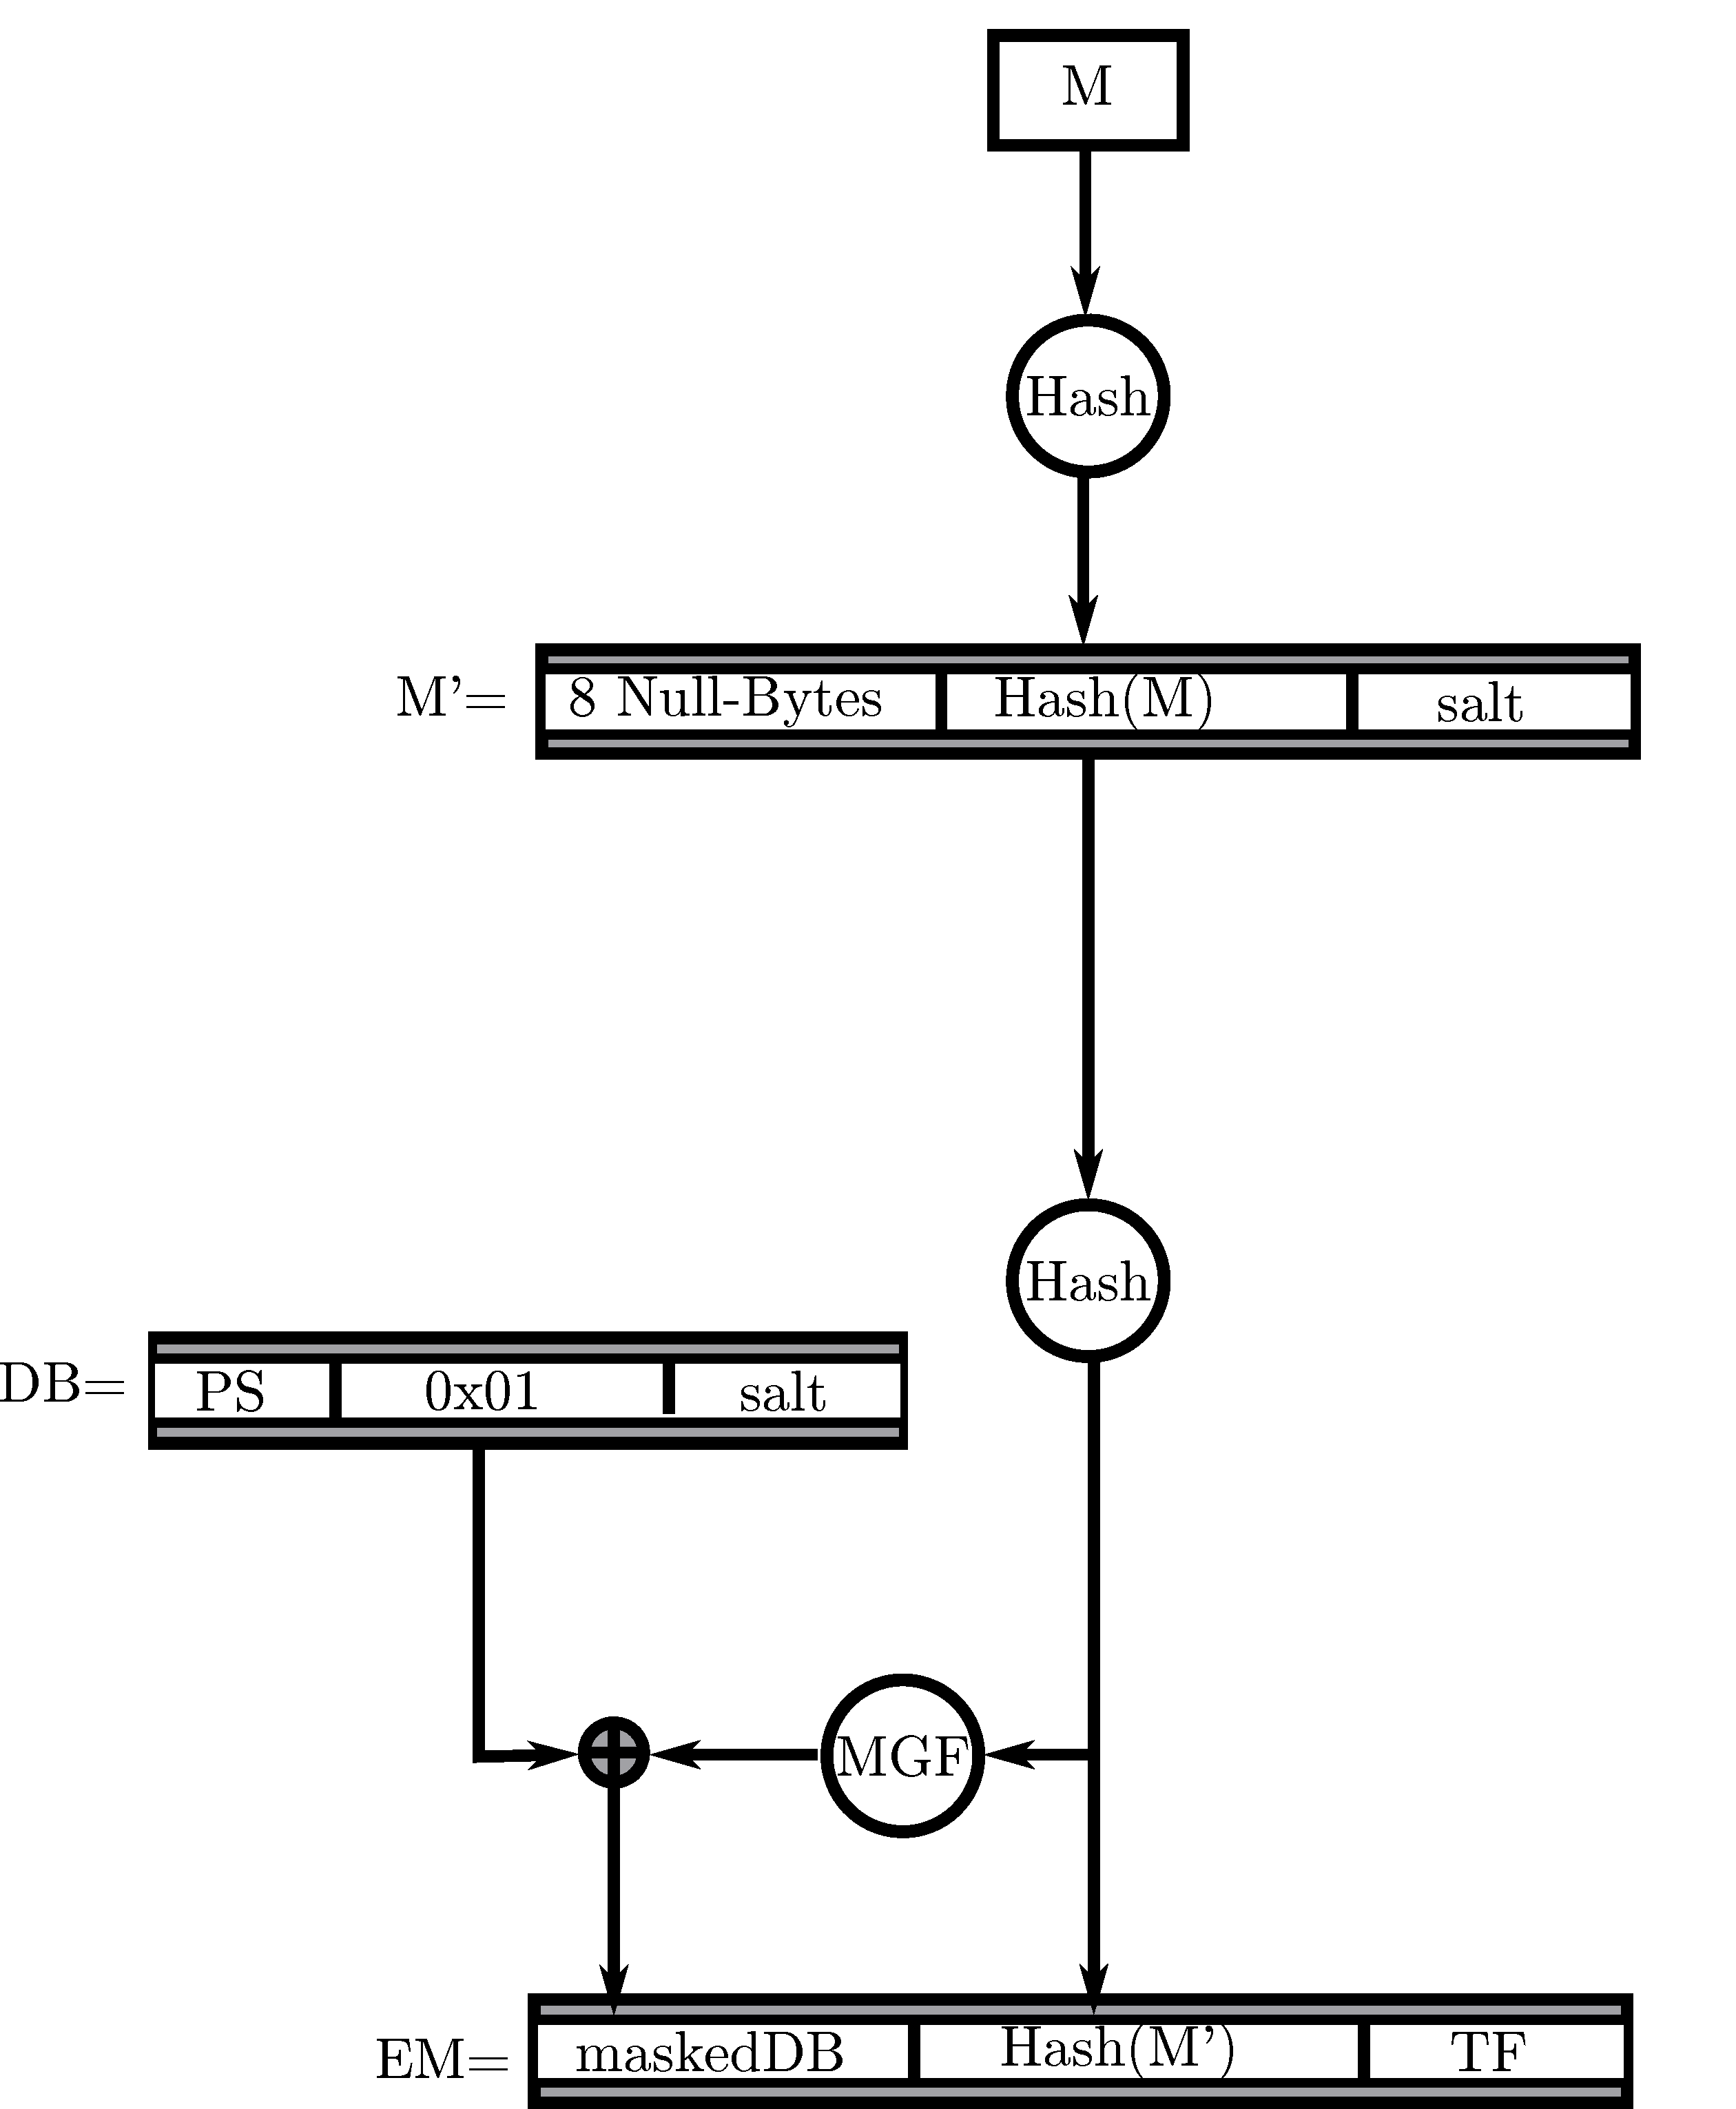
\includegraphics[width=\textwidth]{images/pss.pdf}
    \caption{Padding für RSA-PSS}
    \label{fig:pss}
  \end{subfigure}
  \begin{subfigure}[b]{.45\textwidth}
    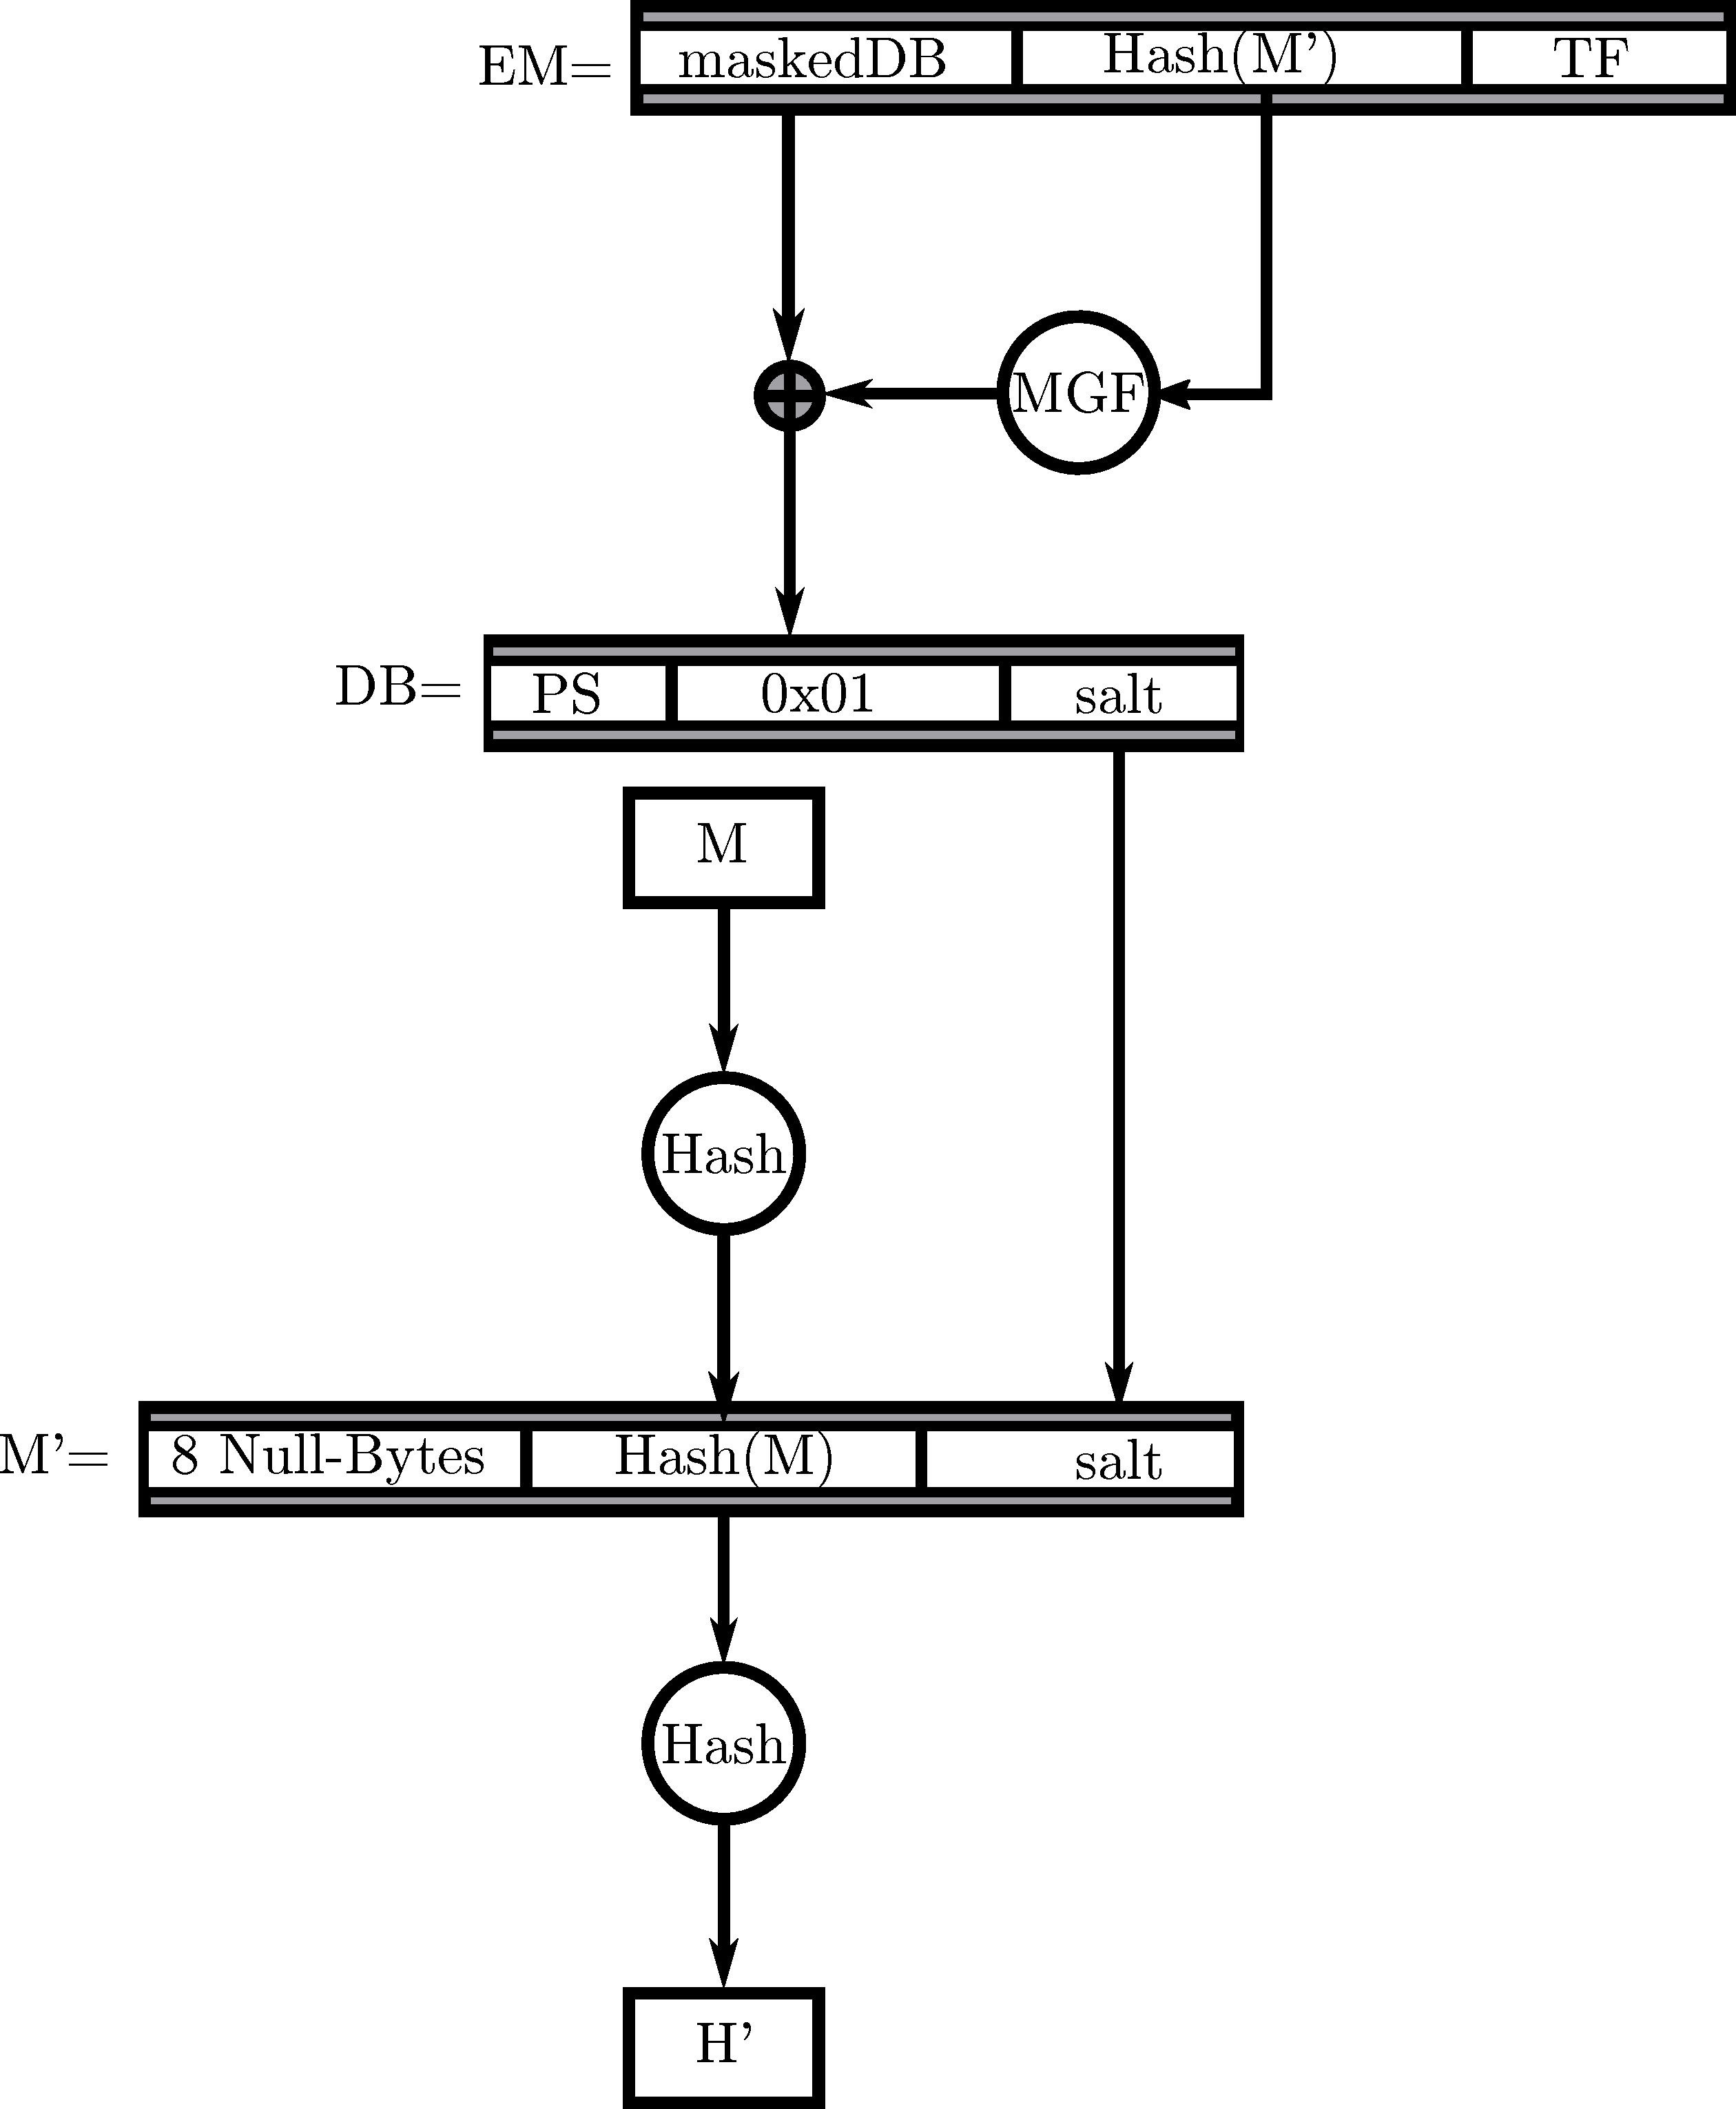
\includegraphics[width=\textwidth]{images/pss-vfy.pdf}
    \caption{Verifikation von gepaddeten Nachrichten}
    \label{fig:pss-vfy}  
  \end{subfigure}
  \caption{Ablauf der Padding-Funktion in RSA-PSS}
\end{figure}


Unter Verwendung idealer Hashfunktionen und mit der Annahme, dass die
RSA-Funktion schwierig zu invertieren ist, ist RSA-PSS heuristisch
EUF-CMA sicher\footnote{D.h. sicher im Random-Oracle-Modell}. Ein Angreifer ist gezwungen, die RSA-Funktion direkt anzugreifen. Der beste bekannte Angriff basiert auf der Faktorisierung von $N$ (unter Verwendung des Zahlkörpersiebs). Die Parameter werden ähnlich wie bei RSA-OAEP gewählt und haben so eine Länge von meistens 2048 Bit. Um eine effiziente Verifikation der Signaturen zu gewährleisten, ist es außerdem ohne Schwierigkeiten möglich, den Parameter $e$ klein zu wählen.


\section{ElGamal}
Analog zum ElGamal-Verschlüsselungssystem aus Kapitel
\ref{ch:asymenc:elgamal} betrachten wir nun ein Signaturverfahren über
der Gruppe $\G = \Z{p}^*$.
\subsection{Erste Idee}
Sei für unseren ersten Versuch der geheime Schlüssel $\skey = (\G, g,
x)$ und der öffentliche Schlüssel $\pkey = (\G, g, g^x)$. Dann bietet
sich die Verwendung von ElGamal zur Erzeugung einer Signatur auf diese
Art an: 
\begin{align*}
\sig(\skey,M) &= a \text{ mit } a \cdot x = M \mod \left|\G\right|\\
\ver(\pkey,\sigma,M) &= 1 :\Leftrightarrow (g^x)^a = g^M
\end{align*}
Allerdings lässt sich diese Konstruktion auf einfache Art brechen, indem
mit $x = M a^{-1} \mod \G$ der geheime Schlüssel berechnet wird. 

\subsection{Schlüssel- und Signaturerzeugung}
Für die Schlüssel gilt weiterhin $\skey = (\G, g,
x)$, $\pkey = (\G, g, g^x)$. 
Für die Signaturerzeugung wird eine zufällige, in $\Z{p}$ invertierbare
Zahl $e \in \{1, \dots, p - 1\}$ gewählt,
wobei $p=|\G|$. Damit berechnet man 
\begin{align*}
a &:= g^e \in \G\\
b &:= (M - a \cdot x) \cdot e^{-1} \mod p
\end{align*}
$a$ wird je nach Kontext als Gruppenelement oder als Zahl interpretiert, $b$
ist eine Zahl in $\Z{p}$.  
Damit gilt $a \cdot x + e \cdot b = M$. Das Signaturverfahren ist nun
$\sig(\skey,M) = (a, b)$.

Für das Verifikationsverfahren werden nun zwei Gruppenelemente $v_1,
v_2 \in \G$ berechnet mit
\begin{align*}
  v_1 &= (g^x)^a \cdot a^b\\
  v_2 &= g^M.
\end{align*}
Das Verifikationsverfahren ist nun
\begin{align*}
\ver(\pkey,\sigma,M) = 1 : & \Leftrightarrow v_1 = v_2 \\
 &\Leftrightarrow (g^x)^a \cdot a^b = g^M \\
 &\Leftrightarrow  g^{ax} \cdot g^{be} = g^M
\end{align*}
Doch auch bei dieser Variante gibt es noch einige offene Angriffspunkte:
\begin{description}
	\item[Doppelte Verwendung von $e$:]
	Wird der zufällige Parameter $e$ mehrmals zur Erzeugung von Signaturen verwendet, kann der geheime Schlüssel $x$ aus den beiden Signaturen errechnet werden. Seien die Signaturen $(a = g^e, b, M)$ und $(a' = g^{e'} = a, b', M')$. Dann ergibt sich durch Aufaddieren und Umformen
	der Gleichungen
	\begin{align*}
	&a \cdot x + e \cdot b = M\\
	\land \quad &a \cdot x + e \cdot b' = M'\\
	\Rightarrow \quad &e = \frac{M - M'}{b - b'}
	\end{align*}
	Mit bekanntem $e$ kann wiederum auf den geheimen Schlüssel $x$
        geschlossen werden.\footnote{Im Signaturverfahren der
          Spielekonsole \textit{PlayStation 3} (PS 3) wurde dem
          Zufallsparameter $e$ ein immer gleicher Wert zugewiesen,
          wodurch der geheime Schlüssel berechnet werden konnte. Dadurch
          wurde es möglich, unautorisierte Anwendungen, wie
          \textit{gecrackte} Spiele, auf der PS 3 auszuführen. Die
          Erklärung zu diesem erfolgreichen Angriff ist
          \href{https://www.youtube.com/watch?v=4loZGYqaZ7I}{hier} zu
          finden, wobei der Angriff auf das Signaturverfahren ab Minute
          35:30 beschrieben wird.} Bei zufälliger Wahl geschieht es nur
        vernachlässigbar oft, dass zwei Mal dasselbe $e$ ausgewählt wird
        und infolgedessen ausgenutzt werden kann .
	\item[Erzeugung "`unsinniger"' Signaturen:]
	Durch günstige Wahl der Parameter ist es möglich, auch ohne Kenntnis des Schlüssels $x$ gültige Signaturen zu erzeugen. Wähle zunächst $c$
	zufällig. Setze außerdem:
	\begin{align*}
	a &:= g^cg^x = g^{c+x}\\
	b &:= -a
	\end{align*}
        Dies impliziert $e=c+x$. 
	Dann ist $(a, b)$ eine gültige Signatur zu $M$ mit
	\begin{align*}
          M &= -ac\\
            &= a \cdot x - a \cdot (c + x)\\
            &= a \cdot x + b \cdot e,\\
	\end{align*}
        denn es gilt 
        \begin{alignat*}{3}
          &&                 & (g^x)^a\cdot a^b       &= &g^M\\
          && \Leftrightarrow & g^{ax} \cdot a^{-a}     &= &g^{-ac}\\
          && \Leftrightarrow & g^{ax} \cdot (g^e)^{-a} &= &g^{-ac}\\
          && \Leftrightarrow & g^{ax-a(c+x)}            &= &g^{-ac}\\
          && \Leftrightarrow & g^{-ac}                 &= &g^{-ac}
        \end{alignat*}
      \end{description}
      \subsection{Beispiel}
      Im Folgenden werden Schlüsselerzeugung, Signieren und Verifizieren beispielhaft
      in der multiplikative Gruppe $\G = \Z{17}^{*}$ mit Ordnung $16$ gezeigt. 
      \subsubsection*{Schlüsselerzeugung}
      Es sind $\skey = (\G, g, x)$ und $\pkey = (\G, g, g^x)$. Als
      Erzeuger wird $g=3$, als Zufallszahl wird $x=11$
      gewählt. Es sind also $\skey = (\G, 3, 11)$ und $\pkey = (\G, 3,
      3^{11})\equiv (\G, 3, 7)$.
      \subsubsection*{Signieren}
      Alice will eine Nachricht $\plaint = 10$ mit $sk$ signieren. Dazu
      wählt sie einen zufälligen, modulo 16 invertierbaren Exponenten
      $e= 13$ und berechnet mit dem erw. Euklidischen Algorithmus
      $e^{-1}=5$. Dann ist $\sigma =  (a, b)$ mit 
      \begin{align*}
       a &:= g^e &\\
         &= 3^{13} \equiv 12 & \mod 17\\
       b &:= (\plaint-a  \cdot x) \cdot e^{-1} & \mod |\G|\\
          &= (10 - 11 \cdot 12) \cdot 13^{-1} & \mod 16\\
          &\equiv (10 - 11\cdot 12) \cdot 5 \equiv 14 & \mod 16
      \end{align*}
      \subsubsection*{Verifizieren}
      Es ist
      \begin{align*}
        v_1 & = (g^x)^a \cdot a^b  & \mod 17 \\
            & = 7^{12} \cdot 12^{14} & \mod 17 \\
            & \equiv 13 \cdot 15 & \mod 17 \\
            & \equiv 8 & \mod 17 \\
        v_2 & = g^M & \mod 17 \\
            &= 3^{10} & \mod 17\\
            &\equiv 8 & \mod 17\\
      \end{align*}
      also gilt $v_1=v_2$ und die Signatur ist gültig.
     

      \section{Hash-Then-Sign-Paradigma}
      Analog zum symmetrischen Fall wollen wir mithilfe des
      Hash-Then-Sign-Paradigmas Nachrichten beliebiger Länge signieren können.
      \begin{theorem}[Hash-Then-Sign-Paradigma]
        Sei $(\keygen, \sig, \ver)$ EUF-CMA-sicher und $H$ eine
        kollisionsresistente Hashfunktion. Dann ist das durch  
        \begin{align*}
          \keygen'(1^k) &= \keygen(1^k)\\
          \sig'(\skey,M) &= \sig(\skey,H(M))\\
          \ver'(\pkey,M,\sigma) &= \ver(\pkey,H(M),\sigma)
        \end{align*}
        definierte Signaturverfahren EUF-CMA-sicher.~\\
      \end{theorem}

      Der Beweis dieses Theorems verläuft analog zu \ref{ch:symauth:eufcma-beweis}.

      Die Verwendung einer kollisionsresistenten Hashfunktion ermöglicht
      eine Abwehr gegen die Erzeugung "`unsinniger"' Signaturen, denn
      die errechneten "`unsinnigen"' Klartexte müssen nun zusätzlich
      denselben Hashwert erzeugen wie die Originalnachricht. 


\section{Digital Signature Algorithm (DSA)}
Aus der Anwendung des Hash-Then-Sign-Paradigmas auf das ElGamal-Signaturverfahren entsteht unter Verwendung einer kollisionsresistenten
Hashfunktion $H$ der \emph{Digital Signature Algorithm} (DSA):
\begin{align*}
a &:= g^e\\
b &:= (H(M) - a \cdot x) \cdot e^{-1} \mod \left|\G\right|
\end{align*}
mit der Signatur $\sigma = (a,b)$.

Der DSA ist nach RSA der zweitwichtigste Signaturalgorithmus und wurde 1994 standardisiert.\footnote{Der aktuelle Standard findet sich auf \url{http://csrc.nist.gov/groups/ST/toolkit/digital_signatures.html}} Für die Bewertung von DSA wirkt sich nachteilig aus, dass für jede neue Signatur eine frische Zufallszahl gewählt werden muss (ein guter Zufallsgenerator wird also
vorausgesetzt) und dass die Verifikation einer DSA-Signatur im Vergleich zu einer RSA-Signatur mit kleinem Modulus deutlich langsamer ist.

Ob DSA EUF-CMA-sicher ist, steht noch nicht eindeutig fest.

\section{Digitale Zertifikate}
Um digital signierte Nachrichten auf ihre Integrität zu prüfen, benötigt
man den öffentlichen Schlüssel. Um sicherzustellen, dass der öffentliche
Schlüssel nicht manipuliert wurde, benutzt man sogenannte PKIs
(\emph{Public Key Infrastructures}). Diese werden oft über digitale
Zertifikate realisiert. Solche Zertifikate werden von einer
sog. \emph{Certificate Authority (CA)} ausgestellt. Überlicherweise
enthalten Zertifikate zumindest
\begin{itemize}
\item den Namen des Ausstellers (\emph{issuer}),
\item den Namen desjenigen, für den das Zertifikat gilt (\emph{subject})
\item einen öffentlichen Schlüssel des \emph{subjects} sowie
\item eine mit dem öffentlichen Schlüssel der CA erstellte Signatur über
  das Zertifikat.
\end{itemize}
Oft werden noch weitere Informationen im Zertifikat gespeichert, wie zum
Beispiel
\begin{itemize}
\item Informationen über das Verfahren, mit dem das Zertifikat generiert wurde,
\item eine Gültigkeitsdauer oder auch
\item Informationen über Rechte des subjects
\end{itemize}

Mithilfe eines solchen Zertifikates kann man sichergehen, dass ein
öffentlicher Schlüssel wirklich zu einer bestimmten Person oder
Institution gehört. Dafür muss man jedoch zum einen der CA trauen, zum
anderen braucht man den öffentlichen Schlüssel der CA. 

Das Vertrauen in die CA ist in vielen Anwendung ein großes Problem. Im
Webbrowser Firefox werden beispielsweise 194 Zertifizierungsstellen
berechtigt, Zertifikate auszustellen\footnote{Stand 28.06.2016. Quelle:
  \url{https://hg.mozilla.org/mozilla-central/raw-file/tip/security/nss/lib/ckfw/builtins/certdata.txt}}. Alle
Zertifiezierungsstellen müssen vertrauenswürdig sein, da sonst
kompromitierte Zertifikate in Umlauf kommen können.

\subsection{X.509}
Der am weitesten verbreitete Standard für Zertifikate ist X.509. Ein
solches Zertifikat findet sich in Abb. \ref{fig:x509}
\begin{figure}
\begin{lstlisting}
Certificate:
    Data:
        Version: 3 (0x2)
        Serial Number: 1 (0x1)
        Signature Algorithm: md5WithRSAEncryption
        Issuer: C=AT, ST=Steiermark, L=Graz, O=TrustMe Ltd,
                OU=Certificate Authority, CN=CA/Email=ca@trustme.dom 
        Validity
            Not Before: Oct 29 17:39:10 2000 GMT
            Not After : Oct 29 17:39:10 2001 GMT
        Subject: C=AT, ST=Vienna, L=Vienna, O=Home, OU=Web Lab,
                 CN=anywhere.com/Email=xyz@anywhere.com 
        Subject Public Key Info:
            Public Key Algorithm: rsaEncryption
            RSA Public Key: (1024 bit)
                Modulus (1024 bit):
                    00:c4:40:4c:6e:14:1b:61:36:84:24:b2:61:c0:b5:
                    d7:e4:7a:a5:4b:94:ef:d9:5e:43:7f:c1:64:80:fd:
                    9f:50:41:6b:70:73:80:48:90:f3:58:bf:f0:4c:b9:
                    90:32:81:59:18:16:3f:19:f4:5f:11:68:36:85:f6:
                    1c:a9:af:fa:a9:a8:7b:44:85:79:b5:f1:20:d3:25:
                    7d:1c:de:68:15:0c:b6:bc:59:46:0a:d8:99:4e:07:
                    50:0a:5d:83:61:d4:db:c9:7d:c3:2e:eb:0a:8f:62:
                    8f:7e:00:e1:37:67:3f:36:d5:04:38:44:44:77:e9:
                    f0:b4:95:f5:f9:34:9f:f8:43
                Exponent: 65537 (0x10001)
        X509v3 extensions:
            X509v3 Subject Alternative Name:
                email:xyz@anywhere.com
            Netscape Comment:
                mod_ssl generated test server certificate
            Netscape Cert Type:
                SSL Server
    Signature Algorithm: md5WithRSAEncryption
        12:ed:f7:b3:5e:a0:93:3f:a0:1d:60:cb:47:19:7d:15:59:9b:
        3b:2c:a8:a3:6a:03:43:d0:85:d3:86:86:2f:e3:aa:79:39:e7:
        82:20:ed:f4:11:85:a3:41:5e:5c:8d:36:a2:71:b6:6a:08:f9:
        cc:1e:da:c4:78:05:75:8f:9b:10:f0:15:f0:9e:67:a0:4e:a1:
        4d:3f:16:4c:9b:19:56:6a:f2:af:89:54:52:4a:06:34:42:0d:
        d5:40:25:6b:b0:c0:a2:03:18:cd:d1:07:20:b6:e5:c5:1e:21:
        44:e7:c5:09:d2:d5:94:9d:6c:13:07:2f:3b:7c:4c:64:90:bf:
        ff:8e
\end{lstlisting}
\caption{Beispiel für ein X.509-Zertifikat}
\label{fig:x509}
\end{figure}

Das Zertifikat ist in zwei Blöcke  unterteilt. Der erste (\texttt{Data})
enthält die Daten, über die das Zertifikate Aussagen macht. Der zweite
Teil (\texttt{Signature Algorithm}) gibt das Verfahren an, mit dem die
Signatur erstellt wurde. Darauf folgt die Signatur.

Der \texttt{Data}-Abschnitt enthält verschiedene Daten:
\begin{itemize}
\item \texttt{Version}: die Version von X509, die verwendet wurde
\item \texttt{Serial Number}: Eine Seriennummer, die für jede CA
  eindeutig sein muss
\item \texttt{Signature Algorithm}: Das Verfahren, mit dem die Signatur
  erstellt wurde.
\item \texttt{Issuer}: Informationen über die CA
\item \texttt{Validity}: Daten, ab wann und bis wann das Zertifikat
  gültig ist
\item \texttt{Subject}: Informationen über die Institution, deren
  öffentlicher Schlüssel zertifiziert wird.
\item \texttt{Subject Public Key Info}: Infomationen über den
  öffentlichen Schlüssel sowie den Schlüssel selbst.
\item \texttt{X509v3 extensions}: Hier kann X509 mit Erweiterungen
  versehen werden, um an besondere Anforderungen angepasst zu werden.
\end{itemize} 
\chapter{Schlüsselaustauschprotokolle}
\label{cha:keyexchange}

In diesem Kapitel widmen wir uns der offenen Frage nach dem
Schlüsselaustauschproblem, das insbesondere bei der Besprechung von
symmetrischen Verschlüsselungs- und Signaturverfahren einige Male
aufgekommen ist. Zwei Kommunikationspartner Alice und Bob können ohne
vorherigen Schlüsselaustausch keine sichere Verbindung
einrichten. Allerdings werden sie nicht jedes Mal die Möglichkeit haben,
sich vor ihrer eigentlichen Kommunikation privat zu treffen, um einen
gemeinsamen Sitzungsschlüssel auszuhandeln. Vielleicht kennen sie
einander nicht einmal persönlich, auf jeden Fall aber wäre ein solches
Vorgehen sichtlich nicht praktikabel.

Alice und Bob müssen also die unsichere Leitung zum Schlüsselaustausch
verwenden. Den Schlüssel im Klartext darüber zu senden, würde einen
Mithörer trivial in die Situation bringen, auch den verschlüsselten Teil
der darauf folgenden Kommunikation mitzulesen. Der neue
Sitzungsschlüssel $\key$ von Alice und Bob muss also bereits so über die
Leitung gesendet werden, dass ein Lauscher nicht in der Lage ist, den
Schlüssel zu rekonstruieren. Dabei sind folgende grundlegende Szenarien
denkbar:\indexSecretKeyInfrastructure \indexPublicKeyInfrastructure
\begin{itemize}
  \item Alice und Bob besitzen bereits einen alten Schlüssel $\key'$ aus
    einem früheren Austausch und möchten ein frisches $\key$ erzeugen
  \item es existierte eine Secret-Key-Infrastruktur mit einer
    Schlüsselzentrale (Alice besitzt einen Schlüssel $\key_A$, Bob $\key_B$
    und die Schlüsselzentrale beide)
  \item es existiert eine Public-Key-Infrastruktur ($\pkey_A, \pkey_B$
    sind öffentlich, Alice besitzt $\skey_A$, Bob besitzt $\skey_B$)
  \item Alice und Bob besitzen ein gemeinsames Passwort
  \item Alice und Bob besitzen keine gemeinsamen Informationen
\end{itemize}


\section{Symmetrische Verfahren}
Als Grundszenario für symmetrische Verfahren wird hier ein System mit
einer Secret-Key-Infrastruktur \indexSecretKeyInfrastructure
gewählt. Das bedeutet, dass jeder Teilnehmer einen geheimen,
symmetrischen Schlüssel mit der Schlüsselzentrale hat. Jeder
Verbindungsaufbau mit einem anderen Teilnehmer beginnt deshalb mit einer
Anfrage an die Zentrale. Da die Zentrale die Anlaufstelle für viele
Teilnehmer ist, sollte die Kommunikation mit dieser Stelle möglichst
minimiert werden, was die vollständige Kommunikation der beiden
Teilnehmer Alice und Bob über die Zentrale ausschließt. Gleichzeitig
sind jedoch die Leitungen nicht vertrauenswürdig, sodass die
Kommunikation über große Strecken verschlüsselt stattfinden sollte.

\subsection{Kerberos}
Eine Lösung für dieses Szenario bietet das Protokoll \emph{Kerberos}
\indexKerberos an, das in Abbildung \ref{fig:keyex:kerberos} in seiner
ursprünglichen Form dargestellt ist. Alice sendet dabei der
Schlüsselzentrale eine Anfrage, die ihren Namen und den ihres
gewünschten Gesprächspartners erhält und bekommt dafür von der Zentrale
zwei Pakete zurück, von denen eines mit ihrem und eins mit Bobs
Schlüssel verschlüsselt ist. Beide Pakete erhalten den gemeinsamen
Sitzungsschlüssel $K$, sowie die Lebensdauer $L$ des Schlüssels und
einen Zeitstempel $T_{KC}$ der Schlüsselzentrale, der Replay-Attacken
erschwert.  Alice entpackt das an sie adressierte Paket, erhält den
Sitzungsschlüssel und leitet nach Prüfung von $L$ und $T$ das für Bob
vorbereitete Paket weiter. Sie fügt außerdem eine mit $K$ verschlüsselte
Nachricht bei, in der sie ihre Identität und einen von ihr erstellten
Zeitstempel $T_A$ einfügt.

Bob überprüft seinerseits den Zeitstempel der Zentrale und die
Lebensdauer des Sitzungsschlüssels und dechiffriert dann Alices
Nachricht mit dem neuen Sitzungsschlüssel. Er kann nun sowohl den
Zeitstempel überprüfen als auch, ob die Anfrage an die Schlüsselzentrale
vom selben Teilnehmer stammt wie die mit dem Sitzungsschlüssel
chiffrierte Nachricht. Außerdem kann er bei erfolgreicher
Entschlüsselung sicher sein, dass Alice $K$ besitzt. Er sendet nun
seinerseits eine mit $K$ verschlüsselte Nachricht an Alice, mit der er
nachweist, dass er den Sitzungsschlüssel besitzt. Mit der Erhöhung des
Zeitstempels kann er außerdem beweisen, dass er die korrekte Nachricht
erhalten und dechiffriert hat.

\begin{figure}[h]
\begin{center}
\unitlength=1mm
\linethickness{0.4pt}
\hspace{-3 cm}
	\begin{picture}(120,60)(-10,0)
		\put(0,53){\makebox(0,0)[cb]{\texttt{Alice}$_{\key_A}$}}
		\put(100,53){\makebox(0,0)[cb]{\texttt{Schlüsselzentrale (KC)$_{\key_A, \key_B}$}}}
		\put(120,28){\makebox(0,0)[cb]{\texttt{Bob$_{\key_B}$}}}
	
		\put(0,2){\line(0,1){50}}
		\put(100,30){\line(0,1){22}}
		\put(120,2){\line(0,1){25}}
		
		\put(50,46){\makebox(0,0)[cb]{(Alice, Bob)}}
		\put(0,45){\vector(1,0){100}}
	
		\put(50,36){\makebox(0,0)[cb]{$\enc(\key_A,(T_{KC}, L, \key, \text{Bob}))$, $\enc(\key_B, (T_{KC}, L, \key, \text{Alice}))$}}
		\put(100,35){\vector(-1,0){100}}
		
		\put(60,20){\makebox(0,0)[cb]{$\enc(\key, (\text{Alice}, T_A))$, $\enc(\key_B, (T_{KC}, L, \key, \text{Alice}))$}}
		\put(0,19){\vector(1,0){120}}
		
		\put(60,10){\makebox(0,0)[cb]{$\enc(K, T_A+1)$}}
		\put(120,9){\vector(-1,0){120}}
	
	\end{picture}
\end{center}
\caption{Ursprüngliches Schlüsselaustauschprotokoll Kerberos. $T_X$ bezeichnet einen von $X$ ausgestellten Zeitstempel, $\key$ den
erzeugten Sitzungsschlüssel für Alice und Bob und $L$ seine Lebensdauer.}
\label{fig:keyex:kerberos}
\end{figure}

Die verschachtelte Konstruktion von Kerberos verhindert
Man-in-the-Middle-Angriffe. Die Kodierung der Absender- und
Empfängernamen durch die Schlüsselzentrale ermöglicht eine
Authentifizierung der Kommunikationsteilnehmer und der Einsatz von
Zeitstempeln sowie die Zuordnung einer Lebensdauer zu einem Schlüssel
erschwert zudem Replay-Attacken.  Nichtsdestotrotz ist für das Protokoll
ein aktiv sicheres Verschlüsselungsverfahren nötig. Die Sicherheit von
Kerberos ist nicht formal geklärt.

\section{Asymmetrische Verfahren}
Als Grundlage für die folgenden Schlüsselaustauschprotokolle nutzen wir
eine Public-Key Infrastruktur. Die Schlüssel werden wie in Kapitel
\ref{ch:asymmenc} von den Teilnehmern selbst erzeugt. Jeder hält also
seinen privaten Schlüssel geheim. Die öffentlichen Schlüssel
hinterliegen an einem allgemein zugänglichen Ort und sind von einer
vertrauenswürdigen Stelle zertifiziert.

\subsection{Public-Key Transport} Das einfachste Verfahren, das sich zum
Schlüsselaustausch in Public-Key-Infrastruktur
\indexPublicKeyInfrastructure anbietet, nennt sich \emph{Public-Key
Transport}\indexPublicKeyTransport. Alice erzeugt einen
Sitzungsschlüssel, den sie für die Kommunikation mit Bob verwenden
will. Die bereits bestehende Infrastruktur wird nun dafür genutzt, den
Sitzungsschlüssel mit Bobs öffentlichem Schlüssel zu chiffrieren und an
Bob zu senden (siehe Abb.
\ref{fig:keyex:publickeytransport}).

\begin{figure}[h]
\begin{center}
\unitlength=1mm
\linethickness{0.4pt}
\hspace{-3 cm}
\begin{picture}(30,10)
\put(0,2){\makebox(0,0)[cb]{$\text{Alice}_{\skey_A}$}}
\put(10,3){\vector(1,0){40}}
\put(30,4){\makebox(0,0)[cb]{$C := \enc(\pkey_B, \key)$}}
\put(55,0.5){\makebox(10,5){$\text{Bob}_{\skey_B}$}}
\end{picture}
\end{center}
\caption{Während des Protokolls Public-Key Transport wählt Alice einen Sitzungsschlüssel $\key$ und sendet ihn unter Ausnutzung der zur
Verfügung stehenden Public-Key-Infrastruktur an Bob.}
\label{fig:keyex:publickeytransport}
\end{figure}

Vorausgesetzt, das verwendete Public-Key-Verfahren ist IND-CPA-sicher,
kann der Angreifer $\ciphert$ nicht von Zufall unterscheiden oder den
darin enthaltenen Sitzungsschlüssel extrahieren. Public-Key Transport
ermöglicht also passive Sicherheit gegenüber einem Angreifer, der
$\ciphert$ auf der Leitung mithören kann.

Allerdings bietet das Verfahren in dieser Form keine Möglichkeit zur
Authentifizierung der Kommunikationsteilnehmer an. Das lässt sich durch
das Hinzufügen von Signaturen wie in Abbildung
\ref{fig:keyex:publickeytransportauth} lösen. Trotzdem ist es dann noch
immer möglich, einen Replay-Angriff durchzuführen und $\ciphert$ zu
einem späteren Zeitpunkt noch einmal zu senden, ohne dass Bob der Fehler
sofort auffällt.

\begin{figure}[h]
\begin{center}
\unitlength=1mm
\linethickness{0.4pt}
\hspace{-3 cm}
\begin{picture}(120,10)(-15,0)
\put(0,0){\makebox(0,0)[cb]{$\text{Alice}_{\skey_{\text{PKE,}A}, \skey_{\sig, A}}$}}
\put(16,3){\vector(1,0){80}}
\put(55,4){\makebox(0,0)[cb]{$(C := \enc(\pkey_{\text{PKE,}B}, \key),$}}
\put(55,-2){\makebox(0,0)[cb]{$\sigma := \sig(\skey_{\sig, A}, C))$}}
\put(110,0){\makebox(10,5){$\text{Bob}_{\skey_{\text{PKE,}B}, \skey_{\sig, B}}$}}
\end{picture}
\end{center}
\caption{Digitale Signaturen ermöglichen den Ausbau des Protokolls Public-Key Transport auf die Authentifikation der Teilnehmer.}
\label{fig:keyex:publickeytransportauth}
\end{figure}


\subsection{Diffie-Hellman-Schlüsselaustausch} 
\label{sec:ddh-key-exchange}\indexDiffieHellmanKeyExchange,
Historisch gesehen entstand das uns schon bekannte
ElGamal-Verschlüsselungsverfahren (1985) aus dem
Diffie-Hellman-Schlüsselaustausch (1976)
den wir im folgenden betrachten werden. Auch hier benötigen wir eine
ausreichend große, zyklische Gruppe $\G = \langle g \rangle$ mit Ordnung
$q$. Alice und Bob wählen sich jeweils eine Zufallszahl $x, y \in
\mathbbm{Z}_q$ und schicken $g^x$ bzw. $g^y$ an den jeweils
anderen. Jeder von beiden ist nun in der Lage, $g^{xy}$ zu
berechnen. Abbildung \ref{fig:keyex:dh} erläutert dies.

Das Berechnen des gemeinsamen Geheimnisses $g^{xy}$ als Außenstehender
bezeichnet man als \emph{computational Diffie-Hellman}-Problem
(CDH-Problem)\indexComputationalDiffieHellmanProblem.  Dabei hat ein
Angreifer Zugriff auf das Erzeugerelement und die beiden Zahlen
$g^{x}$, $g^{y}$. Die Sicherheit des Verfahrens beruht auf der
sogenannten \emph{computational Diffie-Hellman}-Annahme
(CDH-Annahme)\indexComputationalDiffieHellmanAssumption, die besagt,
dass das Lösen des CDH-Problems in manchen zyklischen Gruppen schwer
ist.  Aktive Angriffe, wie Replay- oder Man-in-the-Middle-Attacken, sind
damit allerdings nicht ausgeschlossen.

\begin{figure}[h]
  \begin{center}
    \begin{tikzpicture}[x=2em, y=2em]

      \draw (-6,0) node (Alice) {\texttt{Alice}};
      \draw (-6,-0.5) node (AliceSk) {Geheimnis: $x$};
      \draw (6,0) node (Bob) {\texttt{Bob}};
      \draw (6,-0.5) node (BobSk) {Geheimnis: $y$};
      
      % Lebenslinien
      \draw[dashed] (AliceSk) -- (-6,-3.25);
      \draw[dashed] (BobSk) -- (6,-3.25);
      
      % Pfeile fuer Nachrichten
      \textbf{\draw[->, thick] (-5.7,-1) -- (5.7,-1.5) node[sloped,above,pos=0.5] {$g^x$};}
      \textbf{\draw[->, thick] (5.7,-2.5) -- (-5.7,-3) node[sloped,above,pos=0.5] {$g^y$};}	
      
      % Beschriftung Ergebnis
      \draw (-6, -3.75) node {$(g^y)^x$};
      \draw (-3, -3.75) node {$=$};
      \draw (0, -3.75) node  {$g^{xy}$};
      \draw (3, -3.75) node  {$=$};
      \draw (6, -3.75) node  {$(g^x)^y$};

    \end{tikzpicture}
  \end{center}
  \caption{Diffie-Hellman-Schlüsselaustausch}
  \label{fig:keyex:dh}
\end{figure}
\subsubsection{Man-in-the-Middle-Angriff auf den
  Diffie-Hellman-Schlüsselaustausch}
Man-in-the-Middle-Angriffe sind eine häufige Art von Angriffen gegen
Netzwerkprotokolle. Hierbei versucht ein Angreifer, die Kommunikation
zwischen Alice und Bob dadurch zu übernehmen, dass er die ausgetauschten
Nachrichten abfängt und durch eigene ersetzt.

Im Fall des Diffie-Hellman-Schlüsselaustauschs kann ein Angreifer \A~,
der die Nachrichten manipulieren kann, den Schlüsselaustausch
kompromittieren. Dies wird in Abbildung \ref{fig:keyex:dh-angriff}
dargestellt. Der Angreifer wählt sich einen Zufallswert
$a$ und berechnet $g^a$. Das Ergebnis sendet er dann Alice und Bob, die
ihrerseits $g^x$ bzw. $g^y$ senden. Diese Nachrichten fängt \A~jedoch
ab, sodass Alice und Bob nie die Nachricht der jeweils anderen Partei
erhalten. Somit halten sie das $g^a$ für die Nachricht ihres
Gesprächspartners. Damit werden dann zwei Schlüssel $g^{xa}$ und
$g^{ya}$ erzeugt. Alice und Bob glauben, einen gemeinsamen Schlüssel
ausgetauscht zu haben. Sie haben aber jeweils einen gemeinsamen
Schlüssel mit \A~ausgetauscht.

Angenommen, Alice und Bob würden den Schlüssel nun für ein
Verschlüsselungsverfahren verwenden wollen. Verschlüsselt Alice nun eine
Nachricht, so tut sie dies mit dem Schlüssel $g^{xa}$. Sendet sie also ein
Chiffrat an Bob, so muss \A~dieses abfangen, entschlüsselt (\A~kennt
$g^{xa}$), mit $g^{xb}$ verschlüsseln und dann dieses Chiffrat an Bob
senden. Analog geht \A~vor, wenn Bob eine Nachricht an Alice
schickt. Damit lernt \A~alle Nachrichten, die Alice und Bob
austauschen. Zusätzlich muss \A~dies tun, um nicht aufzufallen. Würde
\A~eine Nachricht nicht so "neuverschlüsseln", so würde Bob bemerken,
dass er das Chiffrat nicht richtig entschlüsseln kann, womit der Angriff
auffällt.

Eine Lösung für dieses Problem ist, dass Alice und Bob ihre Nachrichten
signieren.
\begin{figure}[h]
  \begin{center}
    \scalebox{1}{
      \begin{tikzpicture}[x=2em, y=2em]

        \draw (-6,0) node (Alice) {\texttt{Alice}};
        \draw (-6,-0.5) node (AliceSk) {Geheimnis: $x$};
        \draw (0,0) node (A) {$\mathcal{A}$};
        \draw (6,0) node (Bob) {\texttt{Bob}};
        \draw (6,-0.5) node (BobSk) {Geheimnis: $y$};
        
        \draw[dashed] (AliceSk) -- (-6,-4.25);
        \draw[dashed] (BobSk) -- (6,-4.25);
        
        
        \textbf{\draw[->, thick] (-5.7,-1) -- (-0.3,-1.5) node[sloped,above,pos=0.5] {$g^x$};}
        \textbf{\draw[->, thick] (5.7,-1) -- (0.3,-1.5) node[sloped,above,pos=0.5] {$g^y$};}	
        
        \draw (0,-2.25) node (ASk) {wähle $a$ zufällig};
        \draw[dashed] (A) -- (ASk);	
        \draw[dashed] (ASk) -- (0,-4.25);
        
        \textbf{\draw[->, thick] (-0.3,-3) -- (-5.7,-3.5) node[sloped,above,pos=0.5] {$g^a$};}
        \textbf{\draw[->, thick] (0.3,-3) -- (5.7,-3.5) node[sloped,above,pos=0.5] {$g^a$};}
        
        \draw[decorate, decoration={brace, mirror}] (-5.9,-4) -- node[below=0.4ex] {Schlüssel: $g^{xa}$} (-0.1,-4);
        \draw[decorate, decoration={brace, mirror}] (0.1,-4) -- node[below=0.4ex] {Schlüssel: $g^{ya}$} (5.9,-4);

      \end{tikzpicture}
    }
  \end{center}

  \caption{Man-in-the-Middle-Angriff auf Diffie-Hellman-Schlüsselaustausch}
  \label{fig:keyex:dh-angriff}    
\end{figure}
\section{Transport Layer Security (TLS)}\indexTLS
\label{sec:keyexchange:tls}
TLS (\emph{Transport Layer Security}) ist eine 1999 standardisierte
Weiterentwicklung des von Netscape entwickelten Protokolls SSL
(\emph{Secure Socket Layer}). Das Protokoll besteht aus 5
Teilprotokollen (siehe Tabelle \ref{tbl:tls}). Das Ziel von TLS ist es,
ein sicheres Verschlüsselungsverfahren für die Kommunikation über ein
unsicheres Netzwerk zu ermöglichen

\begin{table}[h]
\centering
\begin{tabular}{lllll}
\cline{1-4}
\multicolumn{1}{|c|}{\begin{tabular}[c]{@{}c@{}}TSL Handshake\\Protocol\end{tabular}} &
\multicolumn{1}{c|}{\begin{tabular}[c]{@{}c@{}}TSL Change Cipher Spec\\Protocol\end{tabular}} &
\multicolumn{1}{c|}{\begin{tabular}[c]{@{}c@{}}TSL Alert\\Protocol\end{tabular}} &
\multicolumn{1}{c|}{\begin{tabular}[c]{@{}c@{}}TSL Application Data\\Protocol\end{tabular}} & \\ \cline{1-4} \multicolumn{4}{|c|}{TLS Record
Protocol} & \\ \cline{1-4} & & & & \\ & & & &
\end{tabular}
\caption{Protokolle in TLS}
\label{tbl:tls}
\end{table}

TLS setzt auf die Transportschicht\indexTransportSchicht des OSI-Modell
auf\footnote{Die 
  Transportschicht ist die 4. Schicht des OSI-Modells, eine in Schichten
  gegliederte Architektur für Netzwerkprotokolle. Auf der 4. Schicht
  sind die bekannten Transportprotokolle TCP und UDP angesiedelt.}
. Dadurch kann TLS unabhängig von Anwendungen auf TCP aufgesetzt
werden. Den Teilprotokollen kommen dabei verschiedene Funktionen zu:
\begin{itemize}
\item Das \emph{TSL Handshake Protocol} initialisiert die
  Verschlüsselung. Dieses Protokoll führt den Schlüsselaustausch durch
  und wird im Folgenden näher betrachtet.
\item Das \emph{TLS Change Cipher Spec Protocol} enthält bloß ein Byte
  mit dem Inhalt \glqq 1\grqq. Dies dient dazu, die ausgehandelte
  Verschlüsselung zu aktivieren.
\item Das \emph{TSL Alert Protocol} meldet Fehler, die im Betrieb
  aufgetreten sind.
\item Das \emph{TSL Record Protocol} ist ein Dummy-Protokoll, dass die
  Daten der Anwendungen weiterreicht.
\item Das \emph{TLS Application Data Protocol} dient dazu, Daten mit den
  ausgehandelten Konfigurationen zu verschlüsseln.
\end{itemize}

\subsection{TLS-Handshake}\indexTLSHandshake 
Der Ablauf des TLS-Handshake-Protokolls ist in Abbildung
\ref{fig:keyex:tls-handshake} vereinfacht dargestellt.

Dafür signalisiert der Client dem Server, dass er den Aufbau eines
verschlüsselten Kanals wünscht (\emph{client\_hello}). Er liefert dem
Server eine Zufallszahl $R_C$ sowie eine nach seiner Präferenz sortierte
Liste von Algorithmen (Hashfunktionen, symmetrische
Verschlüsselungsverfahren und Schlüsselaustauschprotokolle). Der Server
generiert seinerseits eine Zufallszahl $R_S$, wählt einen Satz
Algorithmen aus der Liste des Clients aus und schickt diese zurück
(\emph{server\_hello}). Im Folgenden werden die vom Server ausgewählten
Verfahren verwendet.

Im nächsten Schritt schickt der Server dem Client ein Zertifikat, dass
seinen öffentlichen Schlüssel $pk_S$ enthält, damit der Client
die Identität seines Gesprächspartners überprüfen kann. Haben sich
Client und Server auf beidseitige Authentifikation geeinigt, fordert der
Server außerdem das Zertifikat des Clients an.  Wie genau diese
Authentifizierung abläuft, wurde im vorigen Schritt durch die Auswahl
der entsprechenden Algorithmen festgelegt. Der Client antwortet mit
seinem Zertifikat und seinem öffentlichen Schlüssel $pk_C$. Um die
Integrität der bisherigen Kommunikation sicherzustellen, berechnet der
Client außerdem den Hashwert $H$ der bisher ausgetauschten Nachrichten
und signiert diesen mit seinem privaten Schlüssel. Der Server prüft das
Zertifikat, die Signatur und den Hashwert.

Nun wählt der Client eine weitere Zufallszahl, das so genannte
\emph{premaster secret} (PMS)\indexTLSPreMasterSecret, und schickt es
verschlüsselt mit dem zertifizierten öffentlichen Schlüssel an den
Server. Beide Teilnehmer besitzen nun einen selbst gewählten Zufallswert
sowie einen des Kommunikationspartners und das premaster secret. Aus
diesen drei Zufallszahlen berechnen Client und Server nun mithilfe eines
öffentlich bekannten Algorithmus den \emph{master key}
(MS)\indexTLSMasterKey, aus dem wiederum die für die Kommunikation
verwendeten session keys abgeleitet werden.  Für die Berechnung der
jeweiligen Schlüssel werden Funktionen verwendet, die pseudozufällige
Ergebnisse liefern.

Im letzten Teil des Handshakes signalisiert der Client, dass er nun
verschlüsselt kommunizieren wird (\emph{ChangeCipherSpec}) und dass
damit der Handshake beendet ist (\emph{Finished}). Der Server antwortet
analog. Beide verwenden für die fortlaufende Kommunikation den
vereinbarten Verschlüsselungsalgorithmus und den gemeinsamen session
key.
\begin{figure}[h]
\begin{center}
\unitlength=1mm
\linethickness{0.4pt}
\hspace{-3 cm}
	\begin{picture}(120,150)(-10,0)
		\put(20,143){\makebox(0,0)[cb]{\texttt{Client}$_{\skey_C, \pkey_C}$}}
		\put(100,143){\makebox(0,0)[cb]{\texttt{Server}$_{\skey_S, \pkey_S}$}}
	
		\put(20,2){\line(0,1){140}}
		\put(100,2){\line(0,1){140}}
		
		\put(5,131){\makebox(0,0)[cb]{berechne}}
		\put(5,127){\makebox(0,0)[cb]{Zufallszahl $R_C$}}
		\put(60,123){\makebox(0,0)[cb]{\emph{client\_hello}(Liste$_{Algorithmen}$, $R_C$)}}
		\put(20,122){\vector(1,0){80}}
	
		\put(117,118){\makebox(0,0)[cb]{berechne}}
		\put(117,114){\makebox(0,0)[cb]{Zufallszahl $R_S$}}
		\put(60,110){\makebox(0,0)[cb]{\emph{server\_hello}(Auswahl$_{Algorithmen}$, $R_S$)}}
		\put(100,109){\vector(-1,0){80}}
		
		\put(60,100){\makebox(0,0)[cb]{Server-Zertifikat (inkl. $\pkey_S$)}}
		\put(100,99){\vector(-1,0){80}}
		\put(60,94){\makebox(0,0)[cb]{Anfrage Client-Zertifikat}}
		\put(100,93){\vector(-1,0){80}}
		
		\put(3,87){\makebox(0,0)[cb]{überprüfe}}
		\put(3,84){\makebox(0,0)[cb]{Server-Zertifikat}}
		
		\put(60,80){\makebox(0,0)[cb]{Client-Zertifikat (inkl. $\pkey_C$)}}
		\put(20,79){\vector(1,0){80}}
	
		\put(3,73){\makebox(0,0)[cb]{berechne Hash $H$}}
		\put(3,69){\makebox(0,0)[cb]{aller bisherigen}}
		\put(3,66){\makebox(0,0)[cb]{Nachrichten}}
		\put(60,62){\makebox(0,0)[cb]{$\sig(\skey_C, H)$}}
		\put(20,61){\vector(1,0){80}}
		
		\put(117,55){\makebox(0,0)[cb]{überprüfe $H$}}
		\put(117,51){\makebox(0,0)[cb]{und Signatur}}
		
		\put(3,55){\makebox(0,0)[cb]{berechne}}
		\put(3,51){\makebox(0,0)[cb]{Zufallszahl \emph{PMS}}}
		\put(60,47){\makebox(0,0)[cb]{$\enc(\pkey_S, \textit{PMS})$}}
		\put(20,46){\vector(1,0){80}}
		
		\put(3,40){\makebox(0,0)[cb]{berechne \emph{MS}}}
		\put(3,36){\makebox(0,0)[cb]{aus $R_C$, $R_S$, \emph{PMS}}}
		
		\put(117,40){\makebox(0,0)[cb]{berechne \emph{MS}}}
		\put(117,36){\makebox(0,0)[cb]{aus $R_C$, $R_S$, \emph{PMS}}}
		
		\put(60,32){\makebox(0,0)[cb]{\emph{ChangeCipherSpec}}}
		\put(20,31){\vector(1,0){80}}
		
		\put(60,26){\makebox(0,0)[cb]{\emph{Finished}}}
		\put(20,25){\vector(1,0){80}}
	
		\put(60,16){\makebox(0,0)[cb]{\emph{ChangeCipherSpec}}}
		\put(100,15){\vector(-1,0){80}}
		
		\put(60,10){\makebox(0,0)[cb]{\emph{Finished}}}
		\put(100,9){\vector(-1,0){80}}
	
	\end{picture}
\end{center}
\caption{Vereinfachter Ablauf eines SSL/TLS-Handshakes mit beidseitiger
  Authentifikation.} 
\label{fig:keyex:tls-handshake}
\end{figure}


\subsection{Angriffe auf TLS} Unter Verwendung einer idealen
Verschlüsselung, also im idealen Modell, ist TLS sicher. Auch in der
Praxis gilt die Sicherheit von TLS in der neuesten Version und
Verwendung der richtigen Parameter und Algorithmen als
ausreichend. Allerdings mussten konkrete Implementierungen als Reaktion
auf veröffentlichte Angriffe immer wieder gepatcht werden und es
existieren einige Angriffe auf bestimmte Varianten und Kombinationen von
eingesetzten Algorithmen, von denen im Folgenden einige erklärt werden.

\subsubsection{\texttt{ChangeCipherSpec} Drop} Dieser Angriff entstammt
dem Jahr 1996 und richtet sich gegen SSL unter Version 3.0, also gegen
das Protokoll \emph{vor} seiner Standardisierung als TLS.
\begin{description}
\item[Beobachtung:] Server und Client tauschen zu Beginn ihrer
  Kommunikation eine Reihe unverschlüsselter Nachrichten aus (öffentliche
  Schlüssel, Präferenzen für verwendete Algorithmen, Details der
  Authentifikation \ldots), die es einem Angreifer erlauben, den Status
  des Schlüsselaustauschs zu erkennen. Kurz vor Ende des Handshakes sendet
  der Client, ebenfalls im Klartext, \emph{ChangeCipherSpec}, um auf
  verschlüsselte Kommunikation umzuschalten.
\item[Angriff:] Ein aktiver Angreifer unterdrückt den
  \emph{ChangeCipherSpec}-Hinweis des Clients.
\item[Konsequenz:] Falls der Server sofort danach Nutzdaten
  sendet, werden diese nicht verschlüsselt und können vom Angreifer von
  der Leitung gelesen werden.
\item[Gegenmaßnahme:] Bevor die Nutzdaten gesendet werden, muss
  der Server auf die Bestätigung des Clients warten.
\end{description}

\subsubsection{Beispielangriff auf RSA-Padding} 1998 wurde ein Angriff
auf das RSA-Padding bekannt, der bei entsprechender Algorithmenwahl in
SSL ausgenutzt werden kann, um Einblick in den für die gemeinsame
Kommunikation verwendeten Schlüssel zu erlangen.
\begin{description}
\item[Beobachtung:] Die von SSL eingesetzte Variante von RSA
  verwendet beim Transport des Master Keys \indexTLSMasterKey "`naives"'
  Padding:
  \begin{align*} C = \enc(\pkey, \text{pad}(M)) =
    (\text{pad}(M))^e \mod N
  \end{align*} Dabei kann durch homomorphe Veränderungen
  des Chiffrats $C$ und ständige Überprüfung, ob $C$ noch immer gültig
  ist, auf die Beschaffenheit von $M$ geschlossen werden.
\item[Angriff:] Eine vereinfachte Darstellung des zu
  übertragenden Schlüssels $K$ ist:
  \begin{align*} C = \text{pad}(K)^e =
    (0\mathrm{x}0002 \parallel \mathtt{rnd} \parallel
    0\mathrm{x}00 \parallel K)^e \mod N
  \end{align*} Klar ist, dass $K$ vergleichsweise kurz
  sein und deshalb mit vielen Nullbits beginnen muss. Ziel ist es nun,
  möglichst viele gültige Faktoren $\alpha_i$ zu finden, sodass
  \begin{align*} M_i := \alpha_i \cdot
    (0\mathrm{x}0002 \parallel \mathtt{rnd} \parallel
    0\mathrm{x}00 \parallel K) \mod N = \dec(\alpha_i^e \cdot C \mod N)
  \end{align*} gültig ist. Die Gültigkeit wird
  festgestellt, indem die $M_i$ zur Überprüfung an den Server
  weitergeleitet werden. Der Server gibt in älteren SSL-Versionen
  Hinweise, wenn das Padding fehlerhaft ist.
\item[Konsequenz:] Viele gültige $M_i$ liefern ein grobes
  Intervall, in dem $K$ liegt.
\item[Gegenmaßnahme:] Wähle $K$ zufällig, wenn das Padding
  ungültig ist. (Zu diesem Zeitpunkt stand eigentlich bereits RSA-OAEP zur
  Verfügung.)
\end{description} 
Aus diesem Angriff geht das Theorem von Håstad und Näslund hervor, das
besagt, dass jedes Bit von RSA \emph{hardcore} ist.
\begin{theorem}[Håstad und Näslund] Sei N, e, d wie bei RSA, $M^* \in
\mathbbm{Z}_N$ und $i \in \{1, \ldots , \lfloor \log_2(N)\rfloor \}$
beliebig. Sei $\mathcal{O}$ ein Orakel, das bei Eingabe $C$ das i-te Bit
von $M = C^d \mod N$ ausgibt. Dann existiert ein (von N, e, d
unabhängiger) Polynomialzeit-Algorithmus, der bei Eingabe N, e, i und
$C^* := (M^*)^e \mod N$ und mit $\mathcal{O}$-Zugriff $M^*$ berechnet.
\end{theorem}

\subsubsection{CRIME}
\label{sec:keyex:crime}
Dieser Angriff aus 2002 (Aktualisierung in 2012) funktioniert bei
eingeschalteter Kompression. 
\begin{description}
\item[Beobachtung:] Bei eingeschalteter Kompression wird nicht mehr $M$
  sondern \emph{comp}$(M)$ übertragen. TLS verwendet
  \emph{DEFLATE}-Kompression. Bereits einmal aufgetretene Muster werden
  also nach dem Prinzip \emph{comp}\texttt{(Fliegen fliegen) = Fliegen
    f(-8,6)} wiederverwendet.
\item[Angriff:] Ein Angreifer kann über die Länge des Chiffrats
  feststellen, ob im nachfolgenden (unbekannten) Teil des Klartextes
  Kompression verwendet wurde, indem er einen vorangegangenen Teil
  manipuliert. Die Länge des Chiffrats sinkt dann und der Angreifer weiß,
  dass zumindest ein Teil seines selbst eingefügten Textes im Rest des
  Chiffrats vorgekommen sein muss.
  
  Konkret kann sich ein Angreifer, der in der Lage ist, einem Client
  einen Teil seiner Kommunikation mit dem Server zu diktieren, Stück für
  Stück dem von ihm gesuchten Klartext nähern. Wenn er beispielsweise den
  Session-Cookie des Clients (mit dem geheimen Inhalt \texttt{ABCD})
  stehlen möchte, so kann er (z.B. über Schadcode) dem Client eine Eingabe
  (z.B. \texttt{WXYZ}) diktieren, die dieser vor dem Verschlüsseln der
  Nachricht hinzufügt. Er komprimiert und verschlüsselt also nicht mehr
  nur \texttt{ABCD} sondern \texttt{WXYZABCD}. Aus dem belauschten
  Chiffrat $C := \enc(K, \mathit{comp}(\mathtt{WXYZABCD}))$ kann der
  Angreifer die Länge von $\mathit{comp}(\mathtt{WXYZABCD})$ extrahieren
  und so den Abstand seines eingeschleusten Textstücks \texttt{WXYZ} zu
  dem vom Client geheim gehaltenen Cookie bestimmen.
\item[Konsequenz:] Mit mehreren Wiederholungen kann der Angreifer den
  Inhalt des Cookies immer weiter einschränken und ihn schließlich
  rekonstruieren.
\item[Gegenmaßnahme:] Keine Kompression verwenden.
\end{description}

\subsubsection{Logjam}
Logjam\cite{Adrian2015} ist ein 2015 veröffentlichter Angriff auf das
TLS-Handshake-Protokol. Es ermöglicht einem Man-in-the-Middle-Angreifer
den Server zur Verwendung eines unsicheren Verfahrens zu bringen.
\begin{description}
\item[Beobachtung:] 
  Die ersten Nachrichten des Handshakes sind nicht verschlüsselt. Die
  Absicherung der Integrität wird erst über die Signatur nach dem
  Austausch der Zertifikate erreicht.
\item[Angriff:] Der Angreifer fängt die \emph{client\_hello}-Nachricht ab
  und ersetzt die Liste der Schlüsselaustausch-Verfahren durch eine
  Liste, die lediglich Diffie-Hellman-Schlüsselaustausch mit Schlüsseln
  von 512-bit Länge enthält. Diese manipulierte Nachricht sendet er an
  den Server weiter. Dieser wählt dann das schwache Verfahren aus.
  Der Angreifer hat jetzt bis zum Senden der Signatur über die Hashes
  der bisher gesendeten Nachrichten Zeit, das Verfahren zu brechen und
  an den geheimen Schlüssel zu kommen. Dies braucht zwar einige
  Vorberechnungen, ist aber trotzdem praktikabel.
\item[Konsequenz:] Der Angreifer kann sich als
  Man-in-the-Middle-Angreifer in die verschlüsselte Kommunikation
  einklinken und Nachrichten beliebig manipulieren.
\item[Gegenmaßnahme:] Der Server darf schwache Verschlüsselungen nicht
  akzeptieren, sondern muss den Aufbau von Verbindungen zurückweisen,
  wenn er vom Client lediglich schwache Verfahren vorgeschlagen bekommt.
\end{description}

\subsubsection{Fazit}
TLS \indexTLS ist ein historisch gewachsenes Protokoll mit hoher
Relevanz. Allerdings bietet es durch die hohe Anzahl an Versionen und
Einstellungsmöglichkeiten auch eine große Angriffsfläche, die häufiger
durch Fixes als durch Einführung sichererer Algorithmen reduziert
wird. Dazu kommt, dass von vielen Browsern ausschließlich der
TLS-Standard von 1999 unterstützt wird, was zwar Schwierigkeiten in der
Kompatibilität mit anderen Systemen umgeht, aber auch dazu führt, dass
einige bereits bekannte Ansatzpunkte für Angriffe noch immer
flächendeckend bestehen.

\section{Weitere Protokolle}

\subsection{IPsec}\indexIPsec
IPsec (\emph{Internet Protocol Security}) ist eine Sammlung von
Standards, die zur Absicherung eines IP-Netzwerks entworfen wurden. Es
setzt demnach nicht wie TLS auf der Transportschicht sondern auf der
Internetschicht des TCP/IP-Protokollstapels auf. Es soll die Schutzziele
Vertraulichkeit, Integrität und Authentizität in IP-Netzwerken
sicherstellen. Allerdings liegt der Fokus von IPsec dabei nicht auf dem
Schlüsselaustausch, der deshalb vorher getrennt stattfinden muss
(aktuell durch IKE). Stattdessen bietet IPsec Maßnahmen zur
Integritätssicherung der Daten an (u.A. HMAC), soll die Vortäuschung
falscher IP-Adressen (IP-Spoofing) verhindern und bietet verschiedene
Modi zur Verschlüsselung von IP-Paketen an.

Obwohl IPsec nicht sonderlich stark verbreitet und nicht sehr gut
untersucht ist, haben sich bereits einige Angriffe herauskristallisiert,
auf die hier jedoch nicht näher eingegangen wird.


\subsection{Password Authentication Key Exchange (PAKE)}\indexPAKE
Dieses Protokoll basiert auf der Annahme, dass Alice und Bob, die
miteinander kommunizieren wollen, ein gemeinsames Geheimnis
\texttt{passwort} besitzen. Über dieses Passwort wollen sie einander
authentifizieren und einen Schlüssel für ihre Kommunikation
errechnen. Natürlich kann ein Angreifer trotz allem noch eine
vollständige Suche über die möglichen Passwörter durchführen, es sollte
ihm jedoch nicht möglich sein, schneller ans Ziel zu kommen.

Es handelt sich dabei eher um ein grundlegendes Prinzip als um ein
feststehendes Protokoll. Bei der Konstruktion eines PAKE ist darauf zu
achten, dass die simpelste Variante, das Senden von
$\enc(\mathtt{passwort}, \key)$ keine forward-secrecy bietet. Das
bedeutet, wenn im Nachhinein ein Angreifer das Passwort eines
Teilnehmers knackt, ist er nicht nur zukünftig in der Lage, dessen
Identität zu simulieren sondern kann außerdem sämtliche vergangene
Kommunikation nachvollziehen.

Eine funktionierende Konstruktion ist \emph{Encrypted Key Exchange}
(EKE), bei dem zunächst $\enc(\mathtt{passwort},\pkey)$ gesendet und
infolgedessen asymmetrisch kommuniziert wird. Bei \emph{Simple Password
Exponential Key Exchange} wird ein Diffie-Hellman-Schlüsselaustausch auf
der Basis von einem nur den Teilnehmern bekannten $g =
H(\mathtt{passwort})^2$ durchgeführt. Der beweisbare PAKE von
Goldreich-Lindell nutzt Zero-Knowledge, um die Teilnehmer zu
authentifizieren, ohne das dafür nötige Geheimnis aufzudecken.

PAKE wird z.B. als Basis für EAP (\emph{Extensible Authentication
Protocol}) in WPA verwendet und ist formal modellierbar und seine
Sicherheit unter bestimmten theoretischen Annahmen beweisbar.

\chapter{Identifikationsprotokolle} Nachdem wir jetzt Authentifikation
von Nachrichten und den authentifizierten Austausch von Schlüsseln
betrachtet haben, befasst sich dieses Kapitel mit der asymmetrischen
Identifikation von Kommunikationsteilnehmern. Das bedeutet, Alice ist im
Besitz eines geheimen Schlüssels $\skey$ und Bob, der den dazugehörigen
öffentlichen Schlüssel $\pkey$ kennt, möchte sicher sein, dass er mit
einer Instanz redet, die in Besitz von $\skey$ ist. Üblicherweise geht
es bei dieser Prüfung um den Nachweis einer Identität, der an bestimmte
(Zugangs-)Rechte gekoppelt ist.

Da Alice im Folgenden \emph{beweisen} muss, dass sie den geheimen
Schlüssel besitzt, und Bob ihre Identität \emph{überprüft}, heißen die
beiden für den Rest dieses Kapitels \texttt{Prover} und
\texttt{Verifier}.

Der einfachste Weg, dem Verifier zu beweisen, dass der Prover das
Geheimnis $\skey$ kennt, ist es, ihm den Schlüssel einfach direkt zu
schicken. Der Verifier kann dann die Zugehörigkeit zu $\pkey$
feststellen und sicher sein, dass der Prover das Geheimnis
kennt. Allerdings wird bei diesem Vorgehen $\skey$ allgemein bekannt und
garantiert nach der ersten Verwendung keine Zuordnung mehr zu einer
bestimmten Identität.

Die Protokollanforderungen steigen also darauf, dass der Verifier sicher
sein kann, dass der Prover das Geheimnis kennt, der Verifier selbst
jedoch $\skey$ nicht lernt.

Ein zweiter Versuch umfasst die bereits entwickelten
Signaturschemata. Der Prover schickt $\sigma := \sig(\skey_A,
\text{"`ich bin's, P"'})$ an den Verifier.  $\ver(\pkey_A,\text{"`ich
bin's, P"'}, \sigma)$ liefert dem Verifier die Gültigkeit der
entsprechenden Signatur und damit die Identität des Absenders. Die Idee
hierbei ist, dass der Angreifer eine Signatur fälschen müsste, um das
Identifikationsprotokoll zu brechen, was ein Widerspruch zur Sicherheit
des Signaturverfahrens darstellen würde. Leider funktioniert diese
Argumentation nicht. Ein Angreifer auf das Identifikationsprotokoll
könnte eine bereits gesehene Signatur $\sigma$ wiederverwenden, um sich
gegenüber anderen als den Prover P auszugeben. Dies kann er
beispielsweise in einem Man-in-the-Middle-Angriff oder einer
Replay-Attacke tun.

Aus den ersten beiden Versuchen geht hervor, dass wir ein interaktives
Protokoll wie in Abbildung \ref{fig:id:interaktiv} benötigen, um den
geheimen Schlüssel gleichzeitig zu verbergen und den Besitz dieses
Geheimnisses zu beweisen. Die Sicherheit eines solchen Verfahrens wird
in Kapitel \ref{sec:id:protokolle} näher betrachtet.

\begin{figure}[h]
\begin{center} \unitlength=1mm \linethickness{0.4pt} \hspace{-3 cm}
\begin{picture}(30,20)
\put(10,15){\makebox(0,0)[cb]{$\mathtt{Prover}_{\skey_A}$}}
\put(50,15){\makebox(0,0)[cb]{$\mathtt{Verifier}_{\pkey_A}$}}
    
    \put(10,0){\line(0,1){13}} \put(50,0){\line(0,1){13}}

    \put(50,10){\vector(-1,0){40}} \put(30,11){\makebox(0,0)[cb]{$R$}}
    
    \put(10,3){\vector(1,0){40}} \put(30,4){\makebox(0,0)[cb]{$\sigma :=
\sig(\skey_A, R)$}}
\end{picture}
\end{center}
\caption[foobar]{Interaktives Protokoll, in dem der Verifier dem Prover eine
Zufallszahl $R$ gibt, um dessen Identität durch eine Signatur
sicherzustellen \footnote{Es kann sinnvoll sein,
nicht nur die Zufallszahl $R$ zu signieren, sondern dieser noch das
aktuelle Datum und die aktuelle Uhrzeit hinzuzufügen. So kann, selbst
wenn der Verifier irgendwann zum zweiten Mal die selbe Zufallszahl
ausgibt, eine gerade erzeugte von einer alten Signatur unterschieden
werden.}.}
\label{fig:id:interaktiv}
\end{figure}

\section{Sicherheitsmodell}
\begin{definition}[Public-Key-Identifikationsprotokoll]
Um ein Sicherheitsmodell zu Identifikationsprotokollen betrachten zu
können, definieren wir uns ein solches zunächst formal.
\end{definition}
\begin{definition}
Ein \textit{Public-Key-Identifikationsprotokoll} ist definiert durch ein 3-Tupel
$(\gen, \mathrm{P}, \mathrm{V})$ von PPT-Algorithmen. Dabei gibt $\gen$
wie gewohnt bei Eingabe eines Sicherheitsparameters $1^k$ das
Schlüsselpaar $(\pkey, \skey)$ aus. Der Prover P und der Verifier V sind
zustandsbehaftet und interagieren während des Identitätsnachweises
miteinander.
\end{definition}

Der Ablauf eines solchen Protokolls läuft folgendermaßen ab:
\begin{enumerate}
  \item V erhält den öffentlichen Schlüssel $\pkey$ als Eingabe und
gibt $\mathrm{out}_V$ aus.
  \item P erhält Vs Ausgabe $\mathrm{out}_V$ und gibt $\mathrm{out}_P$ aus.
  \item V erhält Ps Ausgabe $\mathrm{out}_P$ und gibt $\mathrm{out}_V$
    aus.
  \item ist $\mathrm{out}_V \in \{0,1\}$ beende die Interaktion,
    ansonsten springe zurück zu Schritt 2.
\end{enumerate} 

Der Ablauf wird in Abbildung \ref{fig:pki-identifikation} dargestellt.  

\begin{figure}[h]
\begin{center}
    \begin{tikzpicture}[x=1em, y=1em]
      \draw (-6,0) node (P) {$\mathtt{Prover}_{\skey_A}$}; 
      \draw (6,0) node (V) {$\mathtt{Verifier}_{\pkey_A}$};
      
      \draw (P) -- (-6,-6);
      \draw (V) -- (6,-6);
      
      \draw[->] (6 ,-1) -- (-6, -1)
        node[sloped,above, pos=0.5] {$out_{V}$}; 
      
      \draw[->] (-6 ,-3) -- (6, -3)
        node[sloped,above, pos=0.5] {$out_{P}$}; 
      
      \draw[decoration={brace,raise=5pt},decorate] (V) --(6,-3.5)
        node[above, pos=1.3, xshift=55, text width=3cm]{polynomiell oft, wird vom
          Protokoll vorgegeben} (6, -3.5);

      \draw[->] (6 ,-5) -- (-6, -5)
        node[sloped,above, pos=0.5] {$out_V \in \{0, 1\}$}; 
      
    \end{tikzpicture}
  \caption{Ablauf eines Public-Key-Identifikationsprotokolls}
  \label{fig:pki-identifikation}
\end{center}
\end{figure}


Der Verifier erzeugt also eine Ausgabe, mit deren Hilfe
P beweisen muss, dass er das Geheimnis $\skey$ kennt. P liefert auf Basis
des Geheimnisses und der Ausgabe von V seinerseits eine Ausgabe und gibt
diese an V weiter. Möglicherweise tauschen P und V mehrmals wie eben
beschrieben Nachrichten aus. Am Ende prüft V das Ergebnis und
entscheidet, ob die Idendtifikation erfolgreich abgeschlossen wurde. Falls ja,
gibt er 1 aus, falls nein 0. 

% Das Verfahren muss \emph{korrekt} sein, also muss schließlich gelten:
% \begin{align*}
%  \forall (\pkey, \skey) \leftarrow \gen(1^k):
% V(\mathrm{out}_P) \rightarrow 1
% \end{align*}
Das Verfahren muss \emph{korrekt} sein, d.h für alle $(\pkey, \skey)
\leftarrow \gen(1^k)$ wird $V$ am Ende des interaktiven Protokolls mit
$P$ $1$ ausgeben. 
%  $\langle \mathrm{P}(\skey), \mathrm{V}(\pkey) \rangle$
% bezeichnet im Folgenden das Transkript der Interaktion zwischen Prover
% und Verifier.

Einem Angreifer $\A$ darf es nun intuitiv nicht möglich sein, gegenüber
einem Verifier die Identität eines anderen Provers anzunehmen. Um das zu
präzisieren, führen wir ein neues Spiel ein. Zunächst erzeugt der Challenger $i$
$(\pkey, \skey)$-Paare mithilfe des $\gen$-Algorithmus und ordnet die privaten Schlüssel $i$ Provern zu.
\begin{enumerate}
  \item $\A$ darf nun mit beliebig vielen dieser gültigen Prover
interagieren. Dabei nimmt er die Rolle des Verifiers ein und hat demnach
Zugriff auf die passenden öffentlichen Schlüssel $\pkey_i$, während die
gültigen Prover seine Anfragen mit ihren privaten Schlüsseln $\skey_i$
beantworten.
  \item $\A$ wählt sich nun einen der $\pkey_{i}$ aus und gibt sich
    damit gegenüber dem Challenger (welcher nun als \glqq echter\grqq
    Verifier fungiert) als Prover $i$ aus. der Challenger erhält als
    Eingabe $\pkey_i$ von \A.
  \item $\A$ gewinnt, wenn der Challenger als Ergebnis schließlich 1
ausgibt.
\end{enumerate} Wir nennen ein Public-Key-Identifikationsprotokoll
$(\gen, \mathrm{P}, \mathrm{V})$ sicher, wenn kein PPT-Angreifer $\A$
das oben genannte Spiel häufiger als vernachlässigbar oft gewinnt.

Allerdings verhindert das oben genannte Spiel keinen
Man-in-the-Middle-Angriff, in dem $\A$ die Ausgaben einfach
weiterreicht.


\section{Protokolle}\label{sec:id:protokolle}
Mithilfe des eben definierten Sicherheitsbegriffs können wir nun die
Sicherheit des Vorschlags aus Abbildung \ref{fig:id:interaktiv} genauer untersuchen.
Dieser Ansatz basiert auf einem Signaturverfahren. Seine
Sicherheit ist demnach von der Sicherheit des verwendeten
Signaturalgorithmus abhängig.~\\

\begin{theorem} Ist das verwendete Signaturverfahren EUF-CMA-sicher, so
ist das in Abbildung \ref{fig:id:interaktiv} gezeigte
PK-Identifikationsprotokoll $(\gen, \mathrm{P}, \mathrm{V})$ sicher.~\\
\end{theorem}
\begin{beweisidee} Angenommen, es gibt einen Angreifer $A$, der das
PK-Identifikationsprotokoll bricht. Dann ist er in der Lage,
nicht-vernachlässigbar oft aus dem öffentlichen Schlüssel $\pkey_{i^*}$
und einer vom Verifier ausgewählten Zufallszahl $R$ eine Signatur
$\sigma := \sig(\skey_{i^*}, R)$ zu berechnen.

Aus $A$ kann nun ein Angreifer $B$ konstruiert werden, der die
Ergebnisse von $A$ nutzt, um das EUF-CMA-sichere Signaturverfahren zu
brechen.~\\
\end{beweisidee}

Ein weiterer Ansatz für ein funktionierendes Identifikationsprotokoll
auf Public-Key-Basis ist in Abbildung \ref{fig:id:protokoll2}
dargestellt.  Hier wird $R$ vor der Übertragung über die Leitung vom
Verifier mit $\pkey_{i^*}$ verschlüsselt, sodass die Kenntnis von
$\skey_{i^*}$ durch einen Entschlüsselungsvorgang überprüft wird.

Es ist hierbei darauf zu achten, dass das Schlüsselpaar, das für dieses
Identifikationsprotokoll verwendet wird, nicht auch zum Verschlüsseln
gebraucht werden sollte. Ansonsten kann ein Angreifer in der Rolle des
Verifiers die Entschlüsselung von ihm bekannten Chiffraten herbeiführen
und somit jedes beliebige Chiffrat entschlüsseln lassen.

\begin{figure}[h]
\begin{center} \unitlength=1mm \linethickness{0.4pt} \hspace{-3 cm}
    \begin{picture}(50,30)(0,0)
\put(10,22){\makebox(0,0)[cb]{\texttt{Prover}$_{\skey_{i^*}}$}}
\put(10,0){\line(0,1){20}}
    
        \put(70,22){\makebox(0,0)[cb]{\texttt{Verifier}$_{\pkey_{i^*}}$}}
\put(70,0){\line(0,1){20}}
        
        \put(40,16){\makebox(0,0)[cb]{$\ciphert \leftarrow
\enc(\pkey_{i^*}, R)$}} \put(70,15){\vector(-1,0){60}}
        
        \put(40,6){\makebox(0,0)[cb]{$R = \dec(\skey_{i^*}, \ciphert)$}}
\put(10,5){\vector(1,0){60}}
    \end{picture}
\end{center}
\caption{Dieses Identifikationsprotokoll profitiert von der Sicherheit
des verwendeten Public-Key-Verschlüsselungsverfahrens.}
\label{fig:id:protokoll2}
\end{figure}



\begin{theorem} Ist das in Abbildung \ref{fig:id:protokoll2} verwendete
Verschlüsselungsverfahren IND-CCA-sicher, so ist das darauf basierende
PK-Identifikationsprotokoll $(\gen, \mathrm{P}, \mathrm{V})$ sicher.
\end{theorem}

\begin{beweisidee} Der Beweis dafür läuft analog zum obigen. Aus einem
Angreifer $A$, der das Identifikationsprotokoll nicht vernachlässigbar
oft bricht, wird ein Angreifer $B$ konstruiert, der das IND-CCA-sichere
Verschlüsselungsverfahren bricht.
\end{beweisidee}

Identifikationsprotokolle wie die in Abbildungen \ref{fig:id:interaktiv}
und \ref{fig:id:protokoll2} gezeigten heißen auch
"`Challenge-Response-Verfahren"', denn der Verifier stellt dem Prover
eine Aufgabe (oder Herausforderung, die "`Challenge"'), die nur der
echte Prover lösen kann. In dem Protokoll aus Abbildung
\ref{fig:id:interaktiv} ist diese Aufgabe die Erstellung einer Signatur
für einen Zufallsstring~$R$; in Abbildung \ref{fig:id:protokoll2} ist
diese Aufgabe die Entschlüsselung eines zufälligen Chiffrats $C =
\enc(\pkey_{i^*}, R)$. Die Lösung des Provers wird daher auch als die
Antwort, oder "`Response"' bezeichnet.

\chapter{Zero-Knowledge}

Im vorigen Kapitel wurden zwei Voraussetzungen entwickelt, die für Identifikationsprotokolle wünschenswert sind.
\begin{itemize}
  \item Verifier V lernt $\skey_P$ nicht
  \item Prover P beweist, dass er $\skey_P$ kennt
\end{itemize}
Diese Eigenschaften konnten wir im vorigen Kapitel nur teilweise erfüllen. Beispielsweise ist es dem Verifier im Protokoll aus Abbildung
\ref{fig:id:interaktiv} möglich, Teilinformationen über $\skey_P$ zu erlangen. Vielleicht kennt P außerdem nur eine Art Ersatzschlüssel und nicht den echten
$\skey_P$. All das reicht für eine Identifikation aus, kann jedoch dazu führen, dass der geheime Schlüssel mit der Zeit korrumpiert wird.

\section{Zero-Knowledge-Eigenschaften}
Wir wollen nicht nur erreichen, dass V $\skey_P$ nicht lernt, sondern verlangen strikter, dass V \emph{nichts} über den geheimen Schlüssel von
P lernt. Wir müssen dabei allerdings berücksichtigen, dass er in Form von $\pkey_P$ bereits eine mit $\skey_P$ verknüpfte Information besitzt (z.B.
mit $\skey_P = x$ und $\pkey_P = g^x$). Wir verlangen also, dass V während der Kommunikation mit P nichts über $\skey_P$ lernt, was er nicht schon aus $\pkey_P$ berechnen kann.

Wir modellieren dafür zu dem Verifier V einen Simulator $\mathcal{S}$, der dieselbe Ausgabe erzeugt wie V, jedoch ohne mit P kommuniziert zu haben. Dazu benötigen wir die folgende Definition:
\begin{definition}[Ununterscheidbarkeit]
\label{def:zk:ununterscheidbarkeit}
Zwei (möglicherweise vom Sicherheitsparameter $k \in \mathbbm{N}$ abhängige) Verteilungen $X$, $Y$ sind ununterscheidbar (geschrieben $X
\stackrel{c}\approx Y$), wenn für alle PPT-Algorithmen $\A$ die Differenz
\begin{align*}
\Pr \left[ \A(1^k,x) = 1 : x \leftarrow X \right] - \Pr \left[ \A(1^k, y) = 1 : y \leftarrow Y \right]
\end{align*}
vernachlässigbar in $k$ ist.
\end{definition}
Intuitiv sind also Elemente aus $X$ nicht effizient von Elementen aus $Y$ unterscheidbar.

\begin{definition}[Zero-Knowledge]
\label{def:zk}
Ein PK-Identifikationsprotokoll $(\gen, \mathrm{P}, \mathrm{V})$ ist Zero-Knowledge (ZK), falls für jeden PPT-Algorithmus $\A$ (der
Angreifer) ein PPT-Algorithmus $\mathcal{S}$ (der Simulator) existiert, so dass die folgenden Verteilungen ununterscheidbar sind (wobei
$(\pkey, \skey) \leftarrow \gen(1^k)$:
\begin{align*}
\langle \mathrm{P}(\skey), \A(1^k, \pkey) \rangle \text{\qquad und\qquad (Ausgabe von) } \mathcal{S}(1^k, \pkey)
\end{align*}
\end{definition}

$\mathcal{S}$ simuliert also die Interaktion zwischen P und \A. Da $\Sim$ ein PPT-Algorithmus ist, dessen einzige Informationsquelle über $\skey$ der gegebene Public Key $\pkey$ ist, kann die Ausgabe von $\Sim$ nur Informationen enthalten, die bereits mit geringem Aufwand aus $\pkey$ berechnet werden können. Ist die Zero-Knowledge Eigenschaft erfüllt, dann ist ein solches simuliertes Transkript von einem echten Transkript $\langle \mathrm{P}(\skey), \A(1^k, \pkey) \rangle$ nicht unterscheidbar, also kann auch das echte Transkript nicht mehr Informationen über $\skey$ enthalten als bereits in $\pkey$ enthalten sind.

Wir untersuchen nun als Beispiel, ob das oben vorgestellte Identifikationsprotokoll (vgl. Abbildung \ref{fig:id:interaktiv}) ein Zero-Knowledge-Protokoll ist. Im ersten Schritt des Protokolls sendet der Verifier V einen Zufallsstring R an den Prover P. Im zweiten Schritt sendet P eine Signatur der Nachricht R an V zurück.

Um ein glaubwürdiges simuliertes Transkript zu erstellen müsste der Simulator also einen Zufallsstring R und eine gültige Signatur $\sigma := \sig(\skey, R)$ erzeugen, um diese in das simulierte Transkript einzubetten. Das würde aber einen Bruch des Signaturverfahrens erfordern, da $\Sim$ nur über $\pkey$ verfügt. Das Protokoll ist also \emph{nicht} Zero-Knowledge.

Bevor wir jedoch ein Zero-Knowledge-Identifikationsprotokoll vorstellen, benötigen wir noch \emph{Commitments} als Hilfskonstruktion.


\section{Commitments}


Ein Commitment-Schema besteht aus einem PPT-Algorithmus $\Com$. Dieser erhält eine Nachricht $\plaint$ als Eingabe. Außerdem schreiben wir den von $\Com$ verwendeten Zufall $R$ explizit hinzu. Eine Ausführung von $\Com$ wird also als $\Com(\plaint; R)$ geschrieben. Die Ausgabe von $\Com$ wird als \emph{Commitment} bezeichnet. Dieses Commitment muss folgende Eigenschaften erfüllen:
\begin{description}
	\item[Hiding] $\Com(\plaint; R)$ verrät zunächst keinerlei Information über $\plaint$.
	\item[Binding] $\Com(\plaint; R)$ legt den Ersteller des Commitments auf $\plaint$ fest, d.h. der Ersteller kann später nicht glaubhaft behaupten, dass $\plaint' \neq \plaint$ zur Erstellung des Commitments verwendet wurde.
\end{description}

Ein klassisches Anwendungsbeispiel für Commitment-Schemas sind Sportwetten, z.B. auf Pferderennen. Hier möchte Alice eine Wette auf den Ausgang eines Rennens bei der Bank abgeben.
Alice befürchtet jedoch, dass die Bank den Ausgang des Rennens manipulieren könnte, wenn die Bank Alices Wette erfahren würde.
Deshalb möchte Alice ihren Wettschein nicht vor dem Ereignis der Bank übergeben. Andererseits muss die Bank darauf bestehen, dass Alice die Wette vor dem Wettstreit abgibt, denn sonst könnte Alice betrügen, indem sie den Wettschein erst nach Ende des Sportereignisses ausfüllt.

Commitment-Schemas bieten eine einfache Lösung für dieses Dilemma:
Alice setzt ihre Wette $\plaint$ und legt sich mittels des Commitment-Schemas darauf fest. Sie berechnet also ein Commitment $\Com(\plaint;R)$, und händigt dieses der Bank aus.
Wegen der Hiding-Eigenschaft kann die Bank Alices Wette nicht in Erfahrung bringen und deshalb das Rennen nicht gezielt manipulieren. Alice ist also vor Manipulation zu ihren Ungunsten geschützt.
Sobald das Rennen abgeschlossen ist, deckt Alice ihr Commitment auf. Nun erfährt die Bank was Alice gewettet hat und kann ggf. den Gewinn auszahlen.
Die Binding-Eigenschaft des Commitments garantiert der Bank, dass Alice nur ihre echte, vorher gesetzte Wette $\plaint$ aufdecken kann. Damit ist ausgeschlossen, dass Alice die Bank betrügen kann.\\

\begin{definition}[Hiding]
	Ein Commitmentschema $\Com$ ist \emph{hiding}, wenn für beliebige $\plaint \neq \plaint' \in \{0, 1\}^*$ und unabhängig zufälliges $R$ $\Com(\plaint; R) \stackrel{c}{\approx} \Com(\plaint'; R)$
	ist.
\end{definition}

\begin{definition}[Binding]
	Ein Commitmentschema $\Com$ ist \emph{binding}, wenn für jeden PPT-Angreifer $\A$, der $\plaint, R, \plaint', R'$ ausgibt, $\Pr
	\lbrack \Com(\plaint; R) = \Com(\plaint'; R') \text{ und } \plaint \neq \plaint'\rbrack$ vernachlässigbar im Sicherheitsparameter $\secpara$ ist.\\
\end{definition}

In der Literatur existieren verschiedene Konstruktionen für solche Commitment-Verfahren. Ein bekanntes Beispiel sind Pedersen-Commitments \cite{Pedersen1992}.


\section{Beispielprotokoll: Graphendreifärbbarkeit}

Als Beispiel für ein Zero-Knowledge-Identifikationsprotokoll geben wir ein Protokoll an, das auf dem Problem der Dreifärbbarkeit von Graphen beruht. Wir rekapitulieren zunächst dieses Problem.\\

\begin{definition}
Gegeben sei ein Graph $G = (V, E)$ mit Knotenmenge $V$ und Kantenmenge $E \subseteq V^2$. Eine Dreifärbung von $G$ ist eine Abbildung $\phi: V \rightarrow \{1, 2, 3\}$, die jedem Knoten $v \in V$ eine "`Farbe"' $\phi(V) \in \{1,2,3\}$ zuordnet\footnote{Man kann grundsätzlich drei beliebige Farben für die Definition wählen, z.B. "`rot"', "`grün"' und "`blau"'; "`cyan"', "`magenta"' und gelb; oder auch "`pastell"', "`purpur"' und "`pink"'. Die Definition bleibt dabei im Wesentlichen die Gleiche. Um sich um eine konkrete, willkürliche Wahl dieser drei Farben zu drücken verwendet man schlicht 1,2 und 3.}, wobei jede Kante 
$(i, j) \in E$ zwei verschiedenfarbige Knoten $i, j$ verbindet. Es muss also für jede Kante $(i,j)$ gelten, dass $\phi(i) \neq \phi(j)$. Ein Graph $G$ heißt dreifärbbar, wenn eine Dreifärbung für $G$ existiert.\\
\end{definition}
Abbildung \ref{fig:zk:dreifaerbbarkeit} zeigt beispielhaft einen Graphen zusammen mit einer Dreifärbung.\\

\begin{figure}
	\begin{center}
	\unitlength=1mm
	\linethickness{0.4pt}
	\hspace{-3 cm}
	    \begin{picture}(44,44)(-16,-16) 
	    
	    	%Die 7 Knoten			
			\put(0,0){\circle{8}}
			\put(-3,-1){4/1}
			
			\put(12,12){\circle{8}}
			\put( 9,11){3/2}
			
			\put(-12,12){\circle{8}}
			\put(-15,11){2/3}
			
			\put(-12,-12){\circle{8}}
			\put(-15,-13){6/2}
			
			\put(12,-12){\circle{8}}
			\put(9,-13){7/3}
			
			\put(24,0){\circle{8}}
			\put(21,-1){5/1}
			
			\put(0,24){\circle{8}}
			\put(-3,23){1/1}
			
			%Die Verbindungslinien für das innere Quadrat
			\put(-8,12){\line(1,0){16}}
			\put(-8,-12){\line(1,0){16}}
			\put(-12,-8){\line(0,1){16}}
			\put(12,-8){\line(0,1){16}}
			
			%Die Verbindungslinien des innersten Knotens mit den Konten des Quadrats
			\put(-9,-9){\line(1,1){6}}
			\put(9,-9){\line(-1,1){6}}
			\put(3,3){\line(1,1){6}}
			
			%Die Verbindungslinien für die beiden äußersten Knoten
			\put(15,-9){\line(1,1){6}}
			\put(15,9){\line(1,-1){6}}
			\put(-9,15){\line(1,1){6}}
			\put(9,15){\line(-1,1){6}}
	    \end{picture}
	\end{center}
\caption{Ein dreifärbbarer Graph. Für jeden Knoten sind Nummer (links) und Farbe (rechts) angegeben. Da kein Knoten mit einem gleichgefärbten Knoten direkt benachbart ist, ist die hier gezeigte Dreifärbung gültig.}
\label{fig:zk:dreifaerbbarkeit}
\end{figure}

Das Entscheidungsproblem, ob ein gegebener Graph dreifärbbar ist, ist NP-vollständig \cite{Stockmeyer1973}.

Zwar lässt sich für bestimmte Klassen von Graphen $G$ leicht entscheiden, ob sie dreifärbbar sind oder nicht.\footnote{Graphen mit maximalem Knotengrad 2 sind z.B. immer dreifärbbar. Graphen, die eine 4-Clique enthalten (also 4 Knoten, die untereinander alle direkt verbunden sind), sind niemals dreifärbbar.} Es gibt aber auch Wahrscheinlichkeitsverteilungen von Graphen, für die es im Mittel sehr schwierig ist, die Dreifärbbarkeit zu entscheiden. Die Details sind hier für uns nicht weiter interessant.

Wir betrachten nun das folgende Protokoll. Zuvor wird der Algorithmus $\gen$ ausgeführt, der einen zufälligen Graphen $G$ zusammen mit einer Dreifärbung $\phi$ erzeugt. Der öffentliche Schlüssel ist $\pkey = G$, der geheime Schlüssel $\skey = (G, \phi)$.
\begin{enumerate}
	\item Der Prover P wählt eine zufällige Permutation $\pi$ der Farben $\{1,2,3\}$. Mit dieser Permutation werden im nächsten Schritt die Farben von $G$ vertauscht.
	\item Mit dieser Permutation werden nun die Farben von G vertauscht. Anschließend berechnet P für jeden Knoten $i$ das Commitment auf die (neue) Farbe $com_i = \Com(\pi(\phi(i)); R_i)$ und sendet alle Commitments an V, d.h. $P$ legt sich gegenüber V auf den Graphen mit vertauschten Farben fest.
	\item V wählt eine zufällige Kante $(i,j)$ und sendet diese an P.
	\item P öffnet die Commitments $com_i$ und $com_j$ gegenüber V.
	\item V überprüft, ob die Commitments korrekt geöffnet wurden und ob $\pi(\phi(i)) \neq \pi(\phi(j))$. Wenn beides der Fall ist akzeptiert V. Wenn eines nicht der Fall ist, lehnt V ab.
\end{enumerate}

Wenn P ehrlich ist, (also tatsächlich eine Dreifärbung von $G$ kennt), dann kann P V immer überzeugen.
Das bisherigen Protokoll ist aber noch nicht sicher, denn ein Angreifer der keine Dreifärbung von $G$ kennt, könnte einfach eine zufällige Abbildung $\phi': V \rightarrow \{1,2,3\}$ erstellen.
Mit dieser zufälligen Färbung, die im Allgemeinen keine gültige Dreifärbung ist, führt der Angreifer das Protokoll regulär durch, d.h. er wählt eine zufällige Permutation $\pi$ und berechnet die Commitments wie oben angegeben.
Für eine zufällige, vom Verifier gewählte Kante $(i,j)$ gilt dann mit Wahrscheinlichkeit $2/3$ $\phi'(i) \neq \phi'(j)$, also auch $\pi(\phi'(i)) \neq \pi(\phi'(j))$. Der Angreifer kann den Verifier also mit einer Wahrscheinlichkeit von $2/3$ überzeugen.

Diese Schwäche kann man ausräumen, indem man das Protokoll mehrfach ausführt. Der Verifier akzeptiert P nur dann, wenn P in \emph{allen} Durchläufen erfolgreich ist. Scheitert P in auch nur einer einzigen Runde, lehnt V ab. Für das Protokoll mit mehrfacher Wiederholung kann man die Sicherheit auch formal zeigen. Dazu muss man aber natürlich \emph{alle} möglichen Angriffsstrategien betrachten, nicht nur die oben gezeigt Rate-Strategie.\\

Wir möchten uns hier jedoch lieber mit der Zero-Knowledge-Eigenschaft befassen. Zunächst wollen wir dazu an einem Beispiel zeigen, dass der Verifier im obigen Protokoll keine Information über die geheime Dreifärbung $\phi$ von $G$ gewinnt. Im Anschluss werden wir die Zero-Knowledge-Eigenschaft nachweisen.\\

\begin{beispiel}
\label{ex:zk:zkexample}
	Wir betrachten die ersten zwei Runden eines Protokollablaufs zwischen Verifier und Prover. Beide Parteien kennen den öffentlichen Schlüssel, einen Graphen $G = (V, E)$.
	Der Prover kennt den geheimen Schlüssel, eine Dreifärbung $\phi$.
	Es seien $a,b,c \in V$ drei Knoten des Graphen, die mit $\phi(a) = 1$, $\phi(b) = 2$ und $\phi(c) = 3$ gefärbt sind.
	
	Zu Beginn der ersten Runde wählt P die Permutation $\pi_1$ zufällig, hier $\pi_1 = (2, 3, 1)$, also $\pi_1(1) = 2$, $\pi_1(2) = 3$ und $\pi_1(3) = 1$. Anschließend erzeugt P Commitments auf $\pi_1(\phi(i))$ für alle $i \in V$.
	
	Der Verifier wählt eine Kante, hier beispielsweise $(a, b)$, und sendet diese an den Prover. 
	Der Prover öffnet daraufhin die Commitments für die Knoten $a$ und $b$, und so lernt der Verifier $\pi_1(\phi(a)) = 2$ und $\pi_1(\phi(b)) = 3$.
	
	In der nächsten Runde wählt P eine neue, zufällige Permutation $\pi_2$, unabhängig von $\pi_1$. Hier sei $\pi_2 = (2, 1, 3)$. Er erzeugt wieder Commitments $\pi_2(\phi(i))$ für alle $i \in V$, und sendet diese an den Verifier.
	
	Dieser wählt nun seinerseits eine neue, unabhängig zufällige Kante. Dabei tritt zufällig $a$ erneut auf: Die gewählte Kante sei $(a,c)$.
	
	P öffnet also die Commitments für $a$ und $c$. Der Verifier erfährt nun, dass $\pi_2(\phi(a)) = 2$ und $\pi_2(\phi(c)) = 3$ gelten.
	Da hier $\pi_2(\phi(a)) = \pi_1(\phi(a))$ gilt, wurde die Farbe $\phi(a)$ offensichtlich in beiden Runden auf die selbe Farbe, nämlich $2$, abgebildet.
	Tatsächlich ist sogar $\pi_1(\phi(b)) = \pi_2(\phi(c))$. Dadurch erfährt der Verifier jedoch nichts darüber, ob $b$ und $c$ gleich gefärbt sind, denn es könnte sowohl sein dass
	\begin{itemize}
		\item $b$ und $c$ gleich gefärbt sind und P zufällig zwei mal hintereinander die selben Permutation gewählt hat (dann gälte also $\pi_1 = \pi_2$), als auch dass
		\item $b$ und $c$ unterschiedlich gefärbt sind und nur die Permutationen $\pi_1$ und $\pi_2$ unterschiedlich sind.
	\end{itemize}
	Wenn $\pi_1$ und $\pi_2$ unabhängig voneinander gleichverteilt gezogen werden, sind beide Fälle gleich wahrscheinlich.
	Deshalb lernt der Verifier hier \emph{nichts} über die Färbung der Knoten $a, b$ und $c$, und ganz allgemein auch nichts über die vollständige Färbung $\phi$ von $G$.\\
\end{beispiel}

Nach diesem Beispiel zeigen wir nun die Zero-Knowledge-Eigenschaft des Protokolls.
Hierfür müssen wir einen Simulator $\Sim$ angeben, dessen Ausgabe ununterscheidbar von echten Transskripten $\langle \mathrm{P}(\skey), \A(1^k, \pkey) \rangle$ ist.

Um dies zu erreichen, simuliert $\Sim$ intern eine Interaktion mit $\A$. $\Sim$ setzt sich dabei selbst in die Rolle des Provers und setzt $\A$ in die Rolle des Verifiers. $\Sim$ zeichnet dabei alle Ausgaben von $\A$ und sich selbst auf, da diese das auszugebende Transkript bilden.
$\Sim$ verfährt wie folgt:
\begin{enumerate}
	\item \label{item:zk:SimulatorSpeichertZustand}
	$\Sim$ speichert den Zustand von $\A$.
	\item $\Sim$ wählt zufällige Farben $c_i$ für jeden Knoten $i$ und gibt die entsprechenden Commitments gegenüber dem Verifier, also $\A$, ab.
	\item Anschließend simuliert $\Sim$ die weitere Ausführung von $\A$, bis $\A$ eine Kante $(i,j)$ ausgibt.
	
	\item Ist $c_i \neq c_j$, dann deckt $\Sim$ die entsprechenden Commitments für $c_i$ und $c_j$ auf und führt das Protokoll regulär weiter aus.
	
		Ist jedoch stattdessen $c_i = c_j$, dann kann $\Sim$ nicht einfach die Commitments öffnen, denn dann wäre das Transkript offensichtlich von echten Transkripten unterscheidbar: In echten Transkripten werden beim Öffnen der Commitments immer verschiedene Farben gezeigt, in diesem falschen Transkript werden jedoch gleiche Farben aufgedeckt.
		
		Um dennoch ein echt wirkendes Transkript erstellen zu können, setzt $\Sim$ den Algorithmus $\A$ auf den in Schritt \ref{item:zk:SimulatorSpeichertZustand} gespeicherten Zustand zurück, ändert eine der Farben $c_i$ oder $c_j$, gibt dem zurückgesetzten Algorithmus $\A$ nun die entsprechenden neuen Commitments und führt diesen wieder aus.
		
		Nun wird $\A$ wieder $(i,j)$ ausgeben, doch diesmal wird $c_i \neq c_j$ gelten. $\Sim$ kann die Commitments also bedenkenlos öffnen und $\A$ zu Ende ausführen.

			\item Sobald $\A$ terminiert hat gibt $\Sim$ das Transkript der Interaktion von sich selbst und $\A$ aus.
\end{enumerate}

Wir vergleichen nun ein so entstandenes Transkript mit echten Transkripten $\langle \mathrm{P}(\skey), \A(1^k, \pkey) \rangle$.

Ein echtes Transkript besteht aus allen Commitments $com_i$, die eine gültige Dreifärbung des Graphen enthalten, der Wahl $(i,j)$ des Angreifers $\A$, sowie der Information zur Öffnung der Commitments $com_i$ und $com_j$.

Das vom Simulator $\Sim$ ausgegebene Transkript enthält ebenfalls alle Commitments $com_i$, die Wahl des Angreifers $(i,j)$ sowie der Information zur Öffnung der Commitments $com_i$ und $com_j$. Durch die Konstruktion des Simulators werden dabei immer verschiedene Farben aufgedeckt, d.h. in diesem Schritt ist keine Unterscheidung möglich.

Ein Unterschied tritt jedoch bei den Commitments auf: Im echten Protokoll enthalten diese Commitments eine gültige Dreifärbung des Graphen. Im simulierten Transkript enthalten diese eine zufällige Färbung des Graphen, und dies ist im Allgemeinen keine gültige Dreifärbung.
Glücklicherweise lässt sich jedoch wegen der Hiding-Eigenschaft der Commitments nicht effizient feststellen, ob diese eine gültige Dreifärbung oder eine zufällige Färbung des Graphen beinhalten.

Deshalb sind die so entstehenden Transkripte gemäß Definition \ref{def:zk:ununterscheidbarkeit} ununterscheidbar, und die Zero-Knowledge-Eigenschaft (Definition \ref{def:zk}) erfüllt.\\

Mit dem hier gezeigten Protokoll kann man übrigens theoretisch beliebige NP-Aussagen beweisen.
Um für einen beliebigen Bitstring $b$ eine bestimmte Eigenschaft (die als Sprache $L \subset \{0,1\}^*$ aufgefasst werden kann) nachzuweisen, transformiert man das Problem $b \stackrel{?}{\in} L$ in eine Instanz $I$ des Graphdreifärbbarkeitsproblems $L_{G3C}$.
(Dies ist möglich, weil das Graphdreifärbbarkeitsproblem NP-vollständig ist.)
Dann kann man mit obigem Protokoll nachweisen, dass der so entstehende Graph $I$ dreifärbbar ist (also $I \in L_{G3C}$), also $b \in L$ ist.
Der Verifier kann dabei wegen der Zero-Knowledge-Eigenschaft keine Information über $b$ gewinnen, außer das $b \in L$ ist.

Solche Beweise sind zwar extrem ineffizient, aber theoretisch möglich.
Z.B. kann man für zwei Chiffrate $\ciphert_1 = \enc(\pkey, \plaint)$ und $\ciphert_2 = \enc(\pkey, \plaint)$ so nachweisen, dass beide Chiffrate die selbe Nachricht enthalten, ohne die Nachricht preiszugeben.
Dies wird z.B. bei kryptographischen Wahlverfahren benötigt.
Dort werden jedoch effizientere Verfahren verwendet, die aber dann speziell auf ein Verschlüsselungsverfahren zugeschnitten sind.

\section{Proof-of-Knowledge-Eigenschaft}

Nun haben wir gezeigt, dass im vorherigen Protokoll der Verifier \emph{nichts} über $\skey_P$ lernt, was er nicht bereits aus $\pkey_P$ selbst hätte berechnen können.
Nun wenden wir uns der zweiten wünschenswerten Eigenschaft von Identifikationsprotokollen zu: P soll beweisen, dass er tatsächlich $\skey_P$ kennt.

Wir definieren dazu die Proof-of-Knowledge-Eigenschaft:
\begin{definition}(Proof of Knowledge)
	Ein Identifikationsprotokoll $(\gen, P, V)$ ist ein Proof of Knowledge, wenn ein PPT-Algorithmus $\ext$ (der "`Extraktor"') existiert, der bei Zugriff auf einen beliebigen
erfolgreichen Prover P einen
\footnote{Im Allgemeinen kann es mehrere gültige geheime Schlüssel zu einem Public-Key geben. In unserem Beispielprotokoll auf Basis der Graphdreifärbbarkeit ist z.B. jede Permutation einer gültigen Dreifärbung selbst eine gültige Dreifärbung. Es kann darüber hinaus aber auch vorkommen, dass ein Graph zwei verschiedene Dreifärbungen hat, die nicht durch Permutation auseinander hervorgehen.}
geheimen Schlüssel $\skey$ zu $\pkey$ extrahiert.
\end{definition}

Diese Definition scheint zunächst im Widerspruch zur Zero-Knowledge-Eigenschaft zu stehen.
Schließlich forderte die Zero-Knowledge-Eigenschaft doch, dass ein Verifier nichts über $\skey_P$ lernt, während die Proof-of-Knowledge-Eigenschaft fordert, dass man einen vollständigen geheimen Schlüssel aus $P$ extrahieren kann.
Tatsächlich sind diese Eigenschaften jedoch nicht widersprüchlich, da wir dem Extraktor $\ext$ weitergehende Zugriffsmöglichkeiten auf P zugestehen als einem Verifier:
Ein Verifier ist nämlich auf die Interaktion mit P beschränkt, während wir dem Extraktor $\ext$ auch gestatten P zurückzuspulen.

Für unser Graphdreifärbbarkeits-Identifikationsprotokoll können wir diese Eigenschaft auch tatsächlich nachweisen.\\

\begin{theorem}
	Das Graphdreifärbbarkeits-Identifikationsprotokoll ist ein Proof of Knowledge.
\end{theorem}

\begin{beweis}
	Wir geben einen Extraktor $\ext$ an, der einen gültigen $\skey$ extrahiert. Dazu sei P ein beliebiger erfolgreicher Prover.
	
	\begin{enumerate}
		\item Der Extraktor simuliert zunächst einen ehrlichen Verifier V. Er führt P solange aus, bis P die zufällige Farbpermutation $\pi$ gewählt und Commitments $com_i = \Com(\pi(\phi(i));R)$ auf die Farben jedes Knotens abgegeben hat.	
		\item \label{item:zk:ExtraktorSpeichertZustand}
		Nun speichert $\ext$ den Zustand von $P$.
		\item $\ext$ lässt den von ihm simulierten Verifier nun die erste Kante $(i_1, j_1)$ des Graphen $G$ wählen und diese an P übermitteln.
		\item P muss daraufhin die Commitments $com_{i_1}$ und $com_{j_1}$ aufdecken. Der Extraktor lernt also die (vertauschten) Farben der Knoten $i_1$ und $j_1$, nämlich $\pi(\phi(i_1))$ und $\pi(\phi(j_1))$.
		\item Anstatt des Protokoll weiter auszuführen setzt $\ext$ nun P auf den in Schritt \ref{item:zk:ExtraktorSpeichertZustand} zurück. Zu diesem Zeitpunkt hatte P bereits alle Commitments abgegeben und erwartet vom Verifier eine Aufforderung, eine Kante offenzulegen.
		\item $\ext$ wählt nun eine zweite Kante $(i_2, j_2)$ und lässt diese dem Prover vom Verifier übermitteln. Daraufhin deckt P die Commitments $com_{i_2}$ und $com_{j_2}$ auf, und $\ext$ lernt die Farben der Knoten $i_2$ und $j_2$, nämlich $\pi(\phi(i_2))$ und $\pi(\phi(j_2))$.
		\item So verfährt $\ext$ so lange, bis $\ext$ die Farben aller Knoten erfahren hat.
		\footnote{Streng genommen kann der Extraktor hiermit nur die Farben von Knoten in Erfahrung bringen, die mindestens eine Kante haben. Knoten ohne Kanten können jedoch beliebig gefärbt werden, ohne das eine Dreifärbung ihre Gültigkeit verliert.}
		\item Schließlich gibt $\ext$ die Farben $\pi(\phi(i))$ aller Knoten $i$ aus. Da P ein erfolgreicher Prover ist, muss P auch tatsächlich eine gültige Dreifärbung $\phi$ von $G$ besitzen. Dann ist aber auch $\pi \circ \phi$ eine gültige Dreifärbung, und die Ausgabe von $\ext$ damit \emph{ein möglicher} $\skey$ zu $\pkey$.
	\end{enumerate}
\end{beweis}

Der wesentliche Unterschied, warum ein Verifier keinerlei Informationen aus den aufgedeckten Kanten über $\phi$ lernt, ein Extraktor aber schon, ist, dass die dem Verifier aufgedeckten Farben stets einer anderen Permutation unterzogen werden (vgl. Beispiel \ref{ex:zk:zkexample}, während die Kanten, die der Extraktor in Erfahrung bringt immer der selben Permutation unterliegen.

\chapter{Benutzerauthentifikation}\label{cha11}
\index{Benutzerauthentifikation}
In den vorherigen beiden Kapiteln haben wir betrachtet, wie sich ein
Prover gegenüber einem Verifier identifizieren kann.  Dabei konnten wir
durchaus beachtliche Resultate vorweisen.  Leider kommen die bisher
betrachteten Protokolle nur für die computergestützte Identifizierung
des Provers gegenüber dem Verifier in Frage, denn kaum ein Mensch wird
sich einen komplizierten geheimen Schlüssel für ein Signaturverfahren
merken, geschweige denn den Signaturalgorithmus von Hand ausführen
wollen. Man stelle sich dies im Fall von RSA-basierten Signaturen vor:
Alleine der geheime Schlüssel wird eine für 2048-Bit RSA über 600
Stellen lange Zahl sein.  Auch das Protokoll auf Basis der
Graphdreifärbbarkeit ist nur mühsam von Hand auszuführen, da das
Protokoll oft genug wiederholt werden muss, um echte Sicherheit zu
bieten.

Aus diesem Grund wollen wir uns in diesem Kapitel damit
auseinandersetzen, wie sich Menschen authentifizieren (können), und wie
man eine solche Authentifikation möglichst sicher gestalten kann.

\section{Passwörter} \index{Passwörter} 
Die wohl verbreitetste Methode, die Menschen zur Authentifikation
benutzen sind Passwörter. Heutzutage begegnen uns Passwörter fast
überall.  Ob bei Twitter, Facebook, Youtube, in den eigenen
E-Mail-Konten, auf dem eigenen Computer, auf den Computern der
Universität, Amazon, Ebay, in einem Online-Shop oder andernorts, beinahe
überall werden Passwörter verwendet.

Wir modellieren dieses Szenario ganz allgemein: Ein Nutzer $U$ möchte
sich auf einem Server $S$ mittels Passwort $\pw$ einloggen.  Dabei
wünschen wir uns folgende Sicherheitseigenschaften:

\begin{itemize}
	\item Niemand außer $U$ kann sich bei $S$ als $U$ einloggen.
	\item Niemand soll das Passwort $\pw$ erfahren, nach Möglichkeit
auch nicht $S$.
\end{itemize}

Wir betrachten die zwei Angreifer Eve und Mallory. Eve kann die
Kommunikation zwischen $U$ und $S$ abhören, aber nicht
verändern. Mallory hat keinen Zugriff auf diese Kommunikation, ist dafür
jedoch in der Lage, die auf dem Server gespeicherte Benutzerdatenbank zu
erlangen, z.B. in dem er den Server hackt.\footnote{% Es ist übrigens
durchaus keine Seltenheit, dass Hacker Benutzerdatenbanken von gehackten
Webseiten öffentlich ins Internet stellen.  Dies ist besonders dann
gefährlich, wenn Benutzer ihre Passwörter bei anderen Diensten
wiederverwenden.  Noch schlimmer wird es, wenn das Passwort für einen
Benutzeraccount mit der (üblicherweise in Benutzerdatenbanken ebenfalls
hinterlegten) E-Mail-Adresse geteilt wird.  Denn ein solches
E-Mail-Konto kann leicht zum Generalschlüssel zu den Benutzeraccounts
des Opfers bei vielen anderen Webseiten werden.  Dafür muss der
Angreifer nur die "`Passwort Vergessen"'-Funktion auf diesen Webseiten
nutzen.  Häufig erhält der Nutzer dann entweder ein neues Passwort
zugesendet oder erhält eine Möglichkeit, selbst ein neues Passwort zu
wählen.  Hat der Angreifer aber Zugriff auf den E-Mail-Account des
Opfers, so kann er diese Funktion selbst nutzen und sich mit den neuen
Passwörtern auch bei anderen Internetseiten als das Opfer anmelden.  }
Wir betrachten diese Angreifer getrennt, d.h. Eve und Mallory
kooperieren nicht. Sollten sich Eve und Mallory doch zusammentun, so
können sie zusammen mindestens das erreichen, was zuvor schon einer
allein erreichen konnte.

Im einfachsten Verfahren verfügen sowohl $U$ als auch $S$ über das
Passwort $\pw$. Die Authentifikation geschieht, indem $U$ $S$ das
Passwort im Klartext übersendet. Dieses Verfahren ist in Abbildung
\ref{fig:auth:simplepassword} dargestellt.

\begin{figure}[h]
  \begin{center}
    \setlength{\unitlength}{1mm}
    \begin{picture}
      (50,10)(-5,-3) \put(0,-1.25){$U_\pw$}
      \put(45,-1.25){$S_\pw$} \put(8,0){\vector(1,0){36}} \put(23,2.5){$\pw$}
    \end{picture}
  \end{center}
  \caption{Einfache Benutzerauthentifikation mit Passwort.}
  \label{fig:auth:simplepassword}
\end{figure}

Dieses Verfahren bietet jedoch noch keinerlei Sicherheit. Eve, die die
Kommunikation abhören kann, erfährt unmittelbar das Passwort. Auch
Mallory, der die auf $S$ gespeicherte Passwortliste einsehen kann,
erfährt hier das Passwort.

Eine einfache Verbesserung bieten kryptographische Hashfunktionen. Der
Server speichert dann einen Hashwert des Passworts anstatt des Passworts
im Klartext. Dies ist in Abbildung \ref{fig:auth:storedpasswordhash}
gezeigt.

\begin{figure}[h]
  \begin{center} 
    \setlength{\unitlength}{1mm}
    \begin{picture}(50,10)(-5,-3) \put(0,-1.25){$U_\pw$}
      \put(45,-1.25){$S_{H(\pw)}$} \put(8,0){\vector(1,0){36}}
      \put(23,2.5){$\pw$}
    \end{picture}
  \end{center}
  \caption{Einfache Benutzerauthentifikation mit gespeichertem
    Passworthash.}
  \label{fig:auth:storedpasswordhash}
\end{figure}

Der Server kann nun immer noch überprüfen, ob das gesendete Passwort
$\pw$ mit dem gespeicherten Passwort übereinstimmt, indem er den
Hashwert des gesendeten Passworts mit dem gespeicherten Hashwert
vergleicht. Wegen der Kollisionsresistenz der Hashfunktion werden
unterschiedliche Passwörter zu unterschiedlichen Hashwerten führen. Wird
jedoch das richtige Passwort verwendet, so stimmen die Hashwerte
überein.

In diesem Verfahren kann Eve zwar immer noch das Passwort erhalten und
sich damit später als Benutzer $U$ bei $S$ anmelden.  Mallory jedoch,
der nur auf die Benutzerdatenbank von $S$ zugreifen kann, gelangt nur in
Besitz des Passworthashes $H(\pw)$, nicht jedoch von $\pw$ selbst.
Mallory kann sich also gegenüber $S$ nicht als der Benutzer $U$
ausgeben.\footnote{Ist Mallory jedoch ein besonders gewiefter Hacker und
hat Kontrolle über $S$, so könnte er jedoch auch eine Zeit lang alle an
den Server gesendeten Passwörter aufzeichnen und so an eine große Zahl
von Passwörtern gelangen. Meldet sich Benutzer $U$ in dieser Zeit bei
$S$ an, so gelangt Mallory ebenfalls an das Passwort $\pw$.}

In einer weiteren Variante sendet $U$ nicht sein Passwort im Klartext an
$S$, sondern hasht $\pw$ selbst und sendet diesen Hashwert an $S$. Dies
ist in Abbildung \ref{fig:auth:simplehashedpassword} dargestellt.

\begin{figure}[h]
  \begin{center} \setlength{\unitlength}{1mm}
    \begin{picture}(50,10)(-5,-3) \put(0,-1.25){$U_\pw$}
      \put(45,-1.25){$S_{H(\pw)}$} \put(8,0){\vector(1,0){36}}
      \put(21,2.5){$H(\pw)$}
    \end{picture}
  \end{center}
  \caption{Einfache Benutzerauthentifikation mit Hashfunktion und
    Passwort.}
  \label{fig:auth:simplehashedpassword}
\end{figure}

In dieser Variante erfährt Eve zwar nur den Hashwert $H(\pw)$ des
Passworts, dies reicht ihr jedoch, um sich später gegenüber $S$ als $U$
auszugeben. Auch Mallory, der $H(\pw)$ kennt, kann sich später als $U$
bei $S$ anmelden. Dafür erfahren jedoch weder Eve noch Mallory das
tatsächliche Passwort $\pw$. Dies schränkt die Wahrscheinlichkeit, dass
sich Eve oder Mallory bei einem anderen Server anmelden können, bei dem
$U$ das selbe Passwort verwendet, ein.

Die Sicherheitseigenschaften dieser drei einfachen Protokolle sind in
Tabelle \ref{table:auth:overview} zusammengefasst.\\
\begin{table}[h]
  \begin{center}
    \begin{tabular}{l||c|c|c|c} 
      & \multicolumn{2}{c|}{Eve} & \multicolumn{2}{|c}{Mallory}\\ 
      & lernt $\pw$ & Anmelden als $U$ & lernt $\pw$ & Anmelden als $U$
      \\\hline \hline 
      Verfahren 1(Abb. \ref{fig:auth:simplepassword}) & X & X & X & X \\\hline
      Verfahren 2 (Abb. \ref{fig:auth:storedpasswordhash}) & X & X & & \\\hline
      Verfahren 3 (Abb. \ref{fig:auth:simplehashedpassword}) & & X & & X \\
    \end{tabular}
  \end{center}
  \caption{Übersicht über die Sicherheitseigenschaften der drei
    betrachteten Protokolle. Die Spalten "`lernt $\pw$"' geben an, ob der
    jeweilige Angreifer das Passwort $\pw$ direkt lernt. Die Spalten
    "`Anmelden als $U$"' geben an, ob sich der jeweilige Angreifer gegenüber
    $S$ als $U$ ausgeben kann.}
  \label{table:auth:overview}
\end{table}

Man sieht, dass das dritte Verfahren zwar das Passwort $\pw$ besser
schützt als das zweite Verfahren. Dafür eröffnet es Mallory jedoch
wieder die Möglichkeit, sich bei $S$ als $U$ auszugeben.

\section{Wörterbuchangriffe}\index{Wörterbuchangriffe}
Wir betrachten nun noch einmal genauer die Möglichkeiten, aus $H(\pw)$
das benutzte Passwort $\pw$ zu rekonstruieren.

Wegen der Einwegeigenschaft von $H(\pw)$ ist es im Allgemeinen
schwierig, $\pw$ durch "`rückrechnen"' von $H$ zu erhalten. Die
Einwegeigenschaft von $H$ garantiert sogar, dass es sehr schwierig ist,
das Passwort $\pw$ zu finden, wenn das Passwort gleichverteilt zufällig
gewählt wurde.

Unglücklicherweise sind Passwörter jedoch meist alles Andere als
gleichverteilt zufällige Bitstrings.\footnote{ Eine Suche im Internet
fördert verschiedene Listen der am häufigsten benutzten Passwörter
zutage, darunter "`123456"', "`qwertz"' (im englischsprachigen Raum auch
"`qwerty"'), "`password"', oder "`abc123"'; außerdem findet man auch
Programme, die unter Nutzung solcher Listen versuchen, Urbilder zu einer
Liste von Hashes zu finden. Es gibt jedoch auch zahlreiche Anleitungen,
wie gute Passworte erstellt werden können.  }

Natürliche Sprachen wie deutsch oder englisch verfügen nur über wenige
tausend bis zehntausend Worte.  Wird ein solches natürlichsprachliches
Wort als Passwort verwendet, ist es ausreichend alle Worte dieser
Sprache zu hashen und die Hashwerte mit $H(\pw)$ zu vergleichen. Stimmt
der Hashwert eines natürlichen Wortes mit dem bekannten Hashwert
$H(\pw)$ überein, so hat man $\pw$ gefunden.  Es ist also
offensichtlich, dass natürlichsprachliche Worte keine guten Passwörter
sind.

Auch das Verwenden von gebräuchlichen Namen bringt keine wesentliche
Verbesserung, da es auch von diesen nur wenige tausend gibt. Auch das
Anhängen von Ziffern, Geburtstagen oder -jahren ergibt nicht genug
Kombinationsmöglichkeiten, um eine vollständige Suche ausreichend zu
erschweren.

\section{Brute-Force-Angriffe}

Solange also der Vorrat an Passwörtern klein genug ist, ist es mit
relativ wenig Aufwand möglich, zu gegebenem $H(\pw)$ das ursprüngliche
Passwort $\pw$ zu rekonstruieren. Deshalb konzentrieren wir uns nun auf
den Fall, wenn der Vorrat an Passworten sehr groß ist.

In diesem Fall ist es sehr aufwendig, für jeden zu brechenden Hashwert
$H(\pw)$ alle möglichen Passworte durchzuprobieren. Gibt es insgesamt
$N$ Passwörter, dann muss man $H$ etwa $\mathcal{O}(N)$ mal
auswerten. Es ist daher (aus Angreifersicht) wünschenswert, eine
vollständige Liste aller möglichen Passworte $\pw$ und ihrer Hashwerte
$H(\pw)$ zu besitzen. Dies ist in Abbildung \ref{fig:auth:listofhashes}
illustriert.

\begin{figure}[h]
  \begin{align*}
    (\quad H(\pw_1) \qquad&,\qquad \pw_1 \quad) \\
    (\quad H(\pw_2) \qquad&,\qquad \pw_2 \quad) \\ 
    \vdots \qquad&\qquad \vdots
  \end{align*}
  \caption{Eine Liste aller Passwörter und ihrer Hashwerte.}
  \label{fig:auth:listofhashes}
\end{figure}

Ist diese Liste nach $H(\pw)$ sortiert, kann man zu einem gegebenen
Hashwert sogar durch binäre Suche sehr effizient das zugrundeliegende
Passwort bestimmen, man braucht dazu nur $\mathcal{O}(\log_2 N)$
Operationen. Für sehr große Mengen an möglichen Passwörtern werden
jedoch auch diese Listen sehr groß ($\Omega(N)$), und es entsteht ein
Speicherplatzproblem.

\section{Kompression von Hashtabellen/Time Memory Tradeoff}
\index{Hashtabelle}\index{Time-Memory-Tradeoff}
Einen Mittelweg zwischen sehr großer Suchzeit (ohne vorberechnete
Tabelle aller Passworte und Hashwerte) und sehr viel
Speicherplatzverbrauch (mit vollständiger Liste aller Passworte und
ihrer Hashwerte) liefert die Kompression von Hashtabellen. Man
bezeichnet diese Technik auch als "`Time Memory Tradeoff"'.

Unglücklicherweise sind gute, kryptographische Hashwerte quasi zufällig
und nur sehr schwer zu komprimieren. Daher können gängige
Kompressionsverfahren nicht angewendet werden.

Tatsächlich ergibt sich jedoch ein sehr einfaches, maßgeschneidertes
Kompressionsverfahren für solche Hashtabellen, dass sogar eine sehr
effiziente Suche erlaubt.  Hierzu betrachtet man Hash\emph{ketten}.
Eine \emph{Hashkette}\index{Hashkette} (vgl. Abbildung
\ref{fig:auth:hashchain}) beginnt mit einem Passwort $\pw_1$ aus dem
Vorrat aller Passwörter.

Anschließend wird dieses Passwort gehasht, um $H(\pw_1)$ zu erhalten.
Nun wird eine sogenannte \emph{Reduktionsfunktion} $f$ benutzt, um
diesen Hashwert auf ein neues Passwort $\pw_2 = f(H(\pw_1))$ aus dem
Passwortraum abzubilden.  Anschließend wird dieses wieder zu $H(\pw_2)$
gehasht.  Dieser Hashwert wird erneut durch $f$ auf ein Passwort $\pw_3$
abgebildet, usw.  Dieser Prozess kann theoretisch beliebig lange
fortgeführt werden. Man beschränkt dies jedoch auf eine frei wählbare
Anzahl von Iterationen $m$.

\newcommand{\RTF}[1][]{\mathit{f}\if!#1!\else_{#1}\fi}
\newcommand{\VRTF}[1][]{\xlongrightarrow{\RTF[#1]}}
\newcommand{\hasharrow}{\stackrel{H}{\longrightarrow}}
\begin{figure}[h]
  \begin{equation*} \pw_1 \hasharrow H(\pw_1) \VRTF \pw_2
    \hasharrow H(\pw_2) \VRTF %\pw_3 \quad \ldots \quad \hasharrow
    H(\pw_{m-1}) \VRTF \pw_m \hasharrow H(\pw_m)
  \end{equation*}
  \caption{Eine Hashkette.}
  \label{fig:auth:hashchain}
\end{figure}

Eine solche Kette stellen wir auch wie in Abbildung
\ref{fig:auth:hashchainalternative} dar.

\begin{figure}[h]
  \begin{equation*} (H(\pw_{1}),\pw_{1}) \VRTF
    (H(\pw_{2}),\pw_{2}) \VRTF\quad \ldots \quad \VRTF (H(\pw_{m}),\pw_{m})
  \end{equation*}
  \caption{Eine alternative Darstellung für Hashketten.}
  \label{fig:auth:hashchainalternative}
\end{figure}

Es ist leicht einzusehen, dass zur Konstruktion einer solchen Hashkette
nur das Passwort $\pw_1$ benötigt wird. Man kann $\pw_1$ also als stark
komprimierte Form der Hashkette verstehen, da man die gesamte Kette aus
$\pw_1$ berechnen kann.

Anstelle einer vollständigen Liste aller möglichen Passwörter speichert
man nun eine Menge von $n$ Hashketten. Diese kann man tabellarisch wie
in Abbildung \ref{fig:auth:hashchains} darstellen.

\begin{figure}[h]
  \begin{gather*} (H(\pw_{1,1}),\pw_{1,1}) \VRTF
    (H(\pw_{1,2}),\pw_{1,2}) \VRTF\ldots\VRTF (H(\pw_{1,m}),\pw_{1,m})\\
    (H(\pw_{2,1}),\pw_{2,1}) \VRTF (H(\pw_{2,2}),\pw_{2,2}) \VRTF\ldots\VRTF
    (H(\pw_{2,m}),\pw_{2,m})\\ 
    \vdots\\ 
    (H(\pw_{n,1}),\pw_{n,1}) \VRTF
    (H(\pw_{n,2}),\pw_{n,2}) \VRTF\ldots\VRTF (H(\pw_{n,m}),\pw_{n,m})
  \end{gather*}
  \caption{Tabellarische Darstellung von $n$ Hashketten der Länge
    $m$.}
  \label{fig:auth:hashchains}
\end{figure}

Hierbei nimmt man in Kauf, dass möglicherweise nicht alle Passwörter in
der so entstehenden Tabelle auftauchen. Den Anteil dieser Passwörter
kann man jedoch verringern, in dem man die Anzahl der Hashketten $n$
oder die Länge der Hashketten $m$ erhöht.

Um nun eine Kompression der Tabelle bei gleichzeitiger effizienter Suche
zu erreichen, speichert man für jede Hashkette $i$ nur das erste
Passwort $\pw_{i,1}$ und den letzten Hashwert $H(\pw_{i,m})$. Wenn $m
\cdot n$ ungefähr der Zahl aller Passwörter entspricht, dann ist die so
entstehene Tabelle ungefähr um den Faktor $m$ kleiner als eine
vollständige Auflistung aller Passwörter und ihrer Hashwerte.

Tabelle \ref{table:auth:timememorytradeofffinal} zeigt diese "`komprimierte"' Form.
\begin{table}[!h]
  \begin{equation*}
    \begin{array}{|c|c|} \hline \pw_{1,1} & H(\pw_{1,m})\\
      \hline \pw_{2,1} & H(\pw_{2,m})\\
      \hline
      \vdots & \vdots \\
      \hline
      \pw_{n,1} & H(\pw_{n,m})\\
      \hline
    \end{array}
  \end{equation*}
  \caption{Die komprimierte Hashtabelle.}
  \label{table:auth:timememorytradeofffinal}
\end{table}

Diese Tabelle wird nun nach der Spalte der Hashwerte $H(\pw_{i,m})$
sortiert, um eine effiziente Suche nach Hashwerten zu ermöglichen.

Nun sei $H(\pw^*)$ der dem Angreifer bekannte Passworthash. Das Ziel des
Angreifers ist es, mittels der oben gezeigten Tabelle das Passwort
$\pw^*$ zu rekonstruieren.

Zunächst nimmt der Angreifer an, dass das gesuchte Passwort $\pw^*$ als
letztes Passwort in einer der Hashketten auftaucht.  Es soll also $\pw^*
= \pw_{i,m}$ für ein $i$ gelten.  Wenn diese Annahme zutrifft, dann ist
$H(\pw^*)$ also $H(\pw_{i,m})$. Deshalb sucht der Angreifer in der
zweiten Spalte von Tabelle \ref{table:auth:timememorytradeofffinal} nach
$H(\pw^*)$. Dies ist effizient mittels binärer Suche möglich.  War die
Hypothese korrekt, dann liefert diese Suche einen Treffer in der $i$-ten
Zeile. Dann kann der Angreifer die Hashkette von $\pw_{i,1}$ ausgehend
rekonstruieren und erhält so $\pw_{i,m}$. Dies ist das gesuchte Passwort
$\pw^*$. War die Hypothese falsch, dann liefert diese binäre Suche
keinen Treffer.

In diesem Fall stellt der Angreifer eine neue Hypothese auf: "`Das
gesuchte Passwort $\pw^*$ ist als zweitletztes Passwort in einer der
Hashketten enthalten."'  Dann gilt also $\pw^* = \pw_{i,m-1}$ für ein
$i$, und daher auch $H(\pw_{i,m}) = H(f(H(\pw^*)))$, denn $\pw_{i,m}$
ist genau $f(H(\pw_{i,m-1}))$.  Um zu überprüfen, ob diese Hypothese
stimmt, berechnet der Angreifer daher den Hash $H(f(H(\pw^*)))$ und sucht in
Tabelle \ref{table:auth:timememorytradeofffinal} nach dem Ergebnis
dieser Berechnung.  Liefert die Suche einen Treffer in Kette $i$, kann
der Angreifer diese Kette wieder von $\pw_{i,1}$ neu aufbauen und
erfährt so $\pw_{i,m-1} = \pw^*$.  Liefert die Suche keinen Treffer,
dann war die Hypothese falsch, und der Angreifer fährt mit der nächsten
Hypothese fort: das gesuchte Passwort soll als drittletztes in einer der
Hashketten zu finden sein.  Diese Hypothese testet der Angreifer durch
eine Suche nach $H(f(H(f(H(\pw^*)))))$, usw.

Nacheinander testet der Angreifer so alle Positionen in den
Hashketten. Liefert eine der Suchen einen Treffer, so hat der Angreifer
das Passwort gefunden. Andernfalls ist das gesuchte Passwort nicht in
der Hashtabelle enthalten.

\begin{beispiel}
\label{ex:auth:timememorytradeoff} Wir betrachten als Raum aller
möglichen Passwörter die Buchstaben "`a"' bis "`z"'.  Die angewendete
Hashfunktion sei die schon bereits erwähnte SHA-1-Funktion.  Um einen
Hashwert zurück auf ein Passwort abzubilden, interpretieren wir den
Hashwert als natürliche Zahl $h$ in Hexadezimal-Darstellung, und
berechnen $h \mod 26$.  Die so entstehenden Zahlen von $0$ bis $25$
bilden wir auf natürliche Weise zurück auf die Buchstaben "`a"' bis
"`z"' ab.  Wir wählen $m = 4$ als Kettenlänge.  Da es insgesamt 26
mögliche Passwörter gibt, könnte $n = 7$ ausreichen, damit alle
Passworte an irgendeiner Stelle der Hashketten vorkommen, denn insgesamt
gibt es $7 \cdot 4 = 28$ Passwörter in den Hashketten.  Wir wollen es
mit $n = 7$ Hashketten versuchen.

Als Startpassworte der Hashketten wählen wir die Buchstaben "`a"' bis
"`g"'. Die so entstehenden Hashketten sind in Abbildung
\ref{fig:auth:timememorytradeoff:hashchains} gezeigt.

\begin{figure}[h!] 
%complete results: % a =>
%86f7e437faa5a7fce15d1ddcb9eaeaea377667b8 => o \\% b =>
%e9d71f5ee7c92d6dc9e92ffdad17b8bd49418f98 => i \\% c =>
%84a516841ba77a5b4648de2cd0dfcb30ea46dbb4 => w \\% d =>
%3c363836cf4e16666669a25da280a1865c2d2874 => c \\% e =>
%58e6b3a414a1e090dfc6029add0f3555ccba127f => v \\% f =>
%4a0a19218e082a343a1b17e5333409af9d98f0f5 => l \\% g =>
%54fd1711209fb1c0781092374132c66e79e2241b => n \\% h =>
%27d5482eebd075de44389774fce28c69f45c8a75 => d \\% i =>
%042dc4512fa3d391c5170cf3aa61e6a638f84342 => u \\% j =>
%5c2dd944dde9e08881bef0894fe7b22a5c9c4b06 => o \\% k =>
%13fbd79c3d390e5d6585a21e11ff5ec1970cff0c => o \\% l =>
%07c342be6e560e7f43842e2e21b774e61d85f047 => l \\% m =>
%6b0d31c0d563223024da45691584643ac78c96e8 => k \\% n =>
%d1854cae891ec7b29161ccaf79a24b00c274bdaa => w \\% o =>
%7a81af3e591ac713f81ea1efe93dcf36157d8376 => w \\% p =>
%516b9783fca517eecbd1d064da2d165310b19759 => h \\% q =>
%22ea1c649c82946aa6e479e1ffd321e4a318b1b0 => i \\% r =>
%4dc7c9ec434ed06502767136789763ec11d2c4b7 => b \\% s =>
%a0f1490a20d0211c997b44bc357e1972deab8ae3 => d \\% t =>
%8efd86fb78a56a5145ed7739dcb00c78581c5375 => b \\% u =>
%51e69892ab49df85c6230ccc57f8e1d1606caccc => g \\% v =>
%7a38d8cbd20d9932ba948efaa364bb62651d5ad4 => w \\% w =>
%aff024fe4ab0fece4091de044c58c9ae4233383a => q \\% x =>
%11f6ad8ec52a2984abaafd7c3b516503785c2072 => s \\% y =>
%95cb0bfd2977c761298d9624e4b4d4c72a39974a => q \\% z =>
%395df8f7c51f007019cb30201c49e884b46b92fa => m \\
\begin{center}
  \begin{tabular}{c@{$\;\hasharrow\;$}c@{$\;\VRTF\;$}c@{$\;\hasharrow\;$}c@{$\;\VRTF\;$}c@{$\;\hasharrow\;$}c@{$\;\VRTF\;$}c@{$\;\hasharrow\;$}c}
    a & 86f7\ldots & o & 7a81\ldots & w & aff0\ldots & q & 22ea\ldots\\
    b &e9d7\ldots & i & 042d\ldots & u & 51e6\ldots & g & 54fd\ldots\\
    c &84a5\ldots & w & aff0\ldots & q & 22ea\ldots & i & 042d\ldots\\
    d &3c36\ldots & c & 84a5\ldots & w & aff0\ldots & q & 22ea\ldots\\ 
    e &58e6\ldots & v & 7a38\ldots & w & aff0\ldots & q & 22ea\ldots\\
    f &4a0a\ldots & l & 07c3\ldots & l & 07c3\ldots & l & 07c3\ldots\\
    g &54fd\ldots & n & d185\ldots & w & aff0\ldots & q & 22ea\ldots\\
  \end{tabular}
  \caption{Die in Beispiel \ref{ex:auth:timememorytradeoff}
    erzeugten Hashketten. Aus Platzgründen sind die Hashwerte auf die ersten
    vier Hexadezimalstellen gekürzt.}
  \label{fig:auth:timememorytradeoff:hashchains}
\end{center}
\end{figure}

Gespeichert werden von diesen Hashketten nur die Startpassworte sowie
die letzten Hashwerte. Die Tabelle wird nach den Hashwerten
sortiert. Das Ergebnis ist in Tabelle
\ref{table:auth:timememorytradeoff:hashtable} zu sehen.

\begin{table}[h!]
  \begin{center}
    \begin{tabular}{|c|c|} \hline 
      c & 042d\ldots\\ \hline 
      f & 07c3\ldots\\ \hline 
      a & 22ea\ldots\\ \hline 
      d & 22ea\ldots\\ \hline 
      e & 22ea\ldots\\ \hline 
      g & 22ea\ldots\\ \hline 
      b & 54fd\ldots\\ \hline
    \end{tabular}
  \end{center}
  \caption{Die komprimierte Hashtabelle aus Beispiel
    \ref{ex:auth:timememorytradeoff}.}
  \label{table:auth:timememorytradeoff:hashtable}
\end{table}

Der dem Angreifer bekannte Hashwert sei nun $H(\pw^*) = 042d\cdots$.
Der Angreifer stellt nun zunächst die Hypothese auf, dass das gesuchte
Passwort $\pw^*$ als letztes in einer der Hashketten auftaucht. Er sucht
deshalb in Tabelle \ref{table:auth:timememorytradeoff:hashtable} nach
dem ihm bekannten Hashwert $042d\cdots$. Diese Suche liefert einen
Treffer in Zeile $i = 1$. Die Hypothese war also korrekt. Nun weiß der
Angreifer, dass das gesuchte Passwort $\pw^* = \pw_{1,m}$ ist. Er
rekonstruiert also die Hashkette ausgehend vom Startpasswort "`c"' und
erhält so das gesuchte Passwort "`i"'.
\end{beispiel}

\begin{beispiel} Wir betrachten wieder die komprimierte Hashtabelle aus
dem vorherigen Beispiel. Diesmal sei der dem Angreifer bekannte Hashwert
aber $H(\pw^*) = 51e6\ldots$.  Der Angreifer möchte nun testen, ob das
gesuchte Passwort als letztes in einer der Hashketten aus Abbildung
\ref{fig:auth:timememorytradeoff:hashchains} auftritt.  Doch der
gesuchte Hashwert $51e6\ldots$ taucht nicht in der zweiten Spalte von
Tabelle \ref{table:auth:timememorytradeoff:hashtable} auf.  Daher war
diese erste Hypothese falsch. Der Angreifer berechnet $f(H(\pw^*)) = g$
und $H(f(H(\pw^*))) = 54fd\ldots$.  Eine Suche nach diesem Hashwert
liefert tatsächlich einen Treffer in Zeile $i = 7$ der Tabelle
\ref{table:auth:timememorytradeoff:hashtable}.  Der Angreifer
rekonstruiert also die Hashkette ausgehend vom Buchstaben $b$ und erhält
$\pw_{i,m-1} = \pw_{i,3} = u$.  Dies ist das gesuchte Passwort
$\pw^*$.
\end{beispiel}

\begin{beispiel} Wir betrachten wieder die selbe Hashtabelle, diesmal
sei der gesuchte Hashwert jedoch $H(\pw^*) = 7a38\ldots$.  Dieser kommt
in der zweiten Spalte von Tabelle
\ref{table:auth:timememorytradeoff:hashtable} nicht vor, also taucht
$\pw^*$ nicht an der letzten Stelle einer Hashtabelle auf.  Der
Angreifer berechnet daraufhin $f(H(\pw^*)) = w$ und $H(f(H(\pw^*))) =
aff0\ldots$. Auch dieser Hashwert taucht nicht in Tabelle
\ref{table:auth:timememorytradeoff:hashtable} auf, daher ist das
gesuchte Passwort auch nicht als zweitletztes Passwort in einer der
Hashketten enthalten.  Deshalb setzt der Angreifer die Berechnung fort:
er erhält $f(H(f(H(\pw^*)))) = q$ und $H(f(H(f(H(\pw^*))))) =
22ea\ldots$. Dieser Wert taucht gleich vier Mal in Tabelle
\ref{table:auth:timememorytradeoff:hashtable} auf. Der Angreifer
rekonstruiert daher die vier Ketten ausgehend von "`a"', "`d"', "`e"'
und "`g"', und findet schließlich in der von "`e"' ausgehenden Hashkette
das gesuchte Passwort "`v"'.
\end{beispiel}

Dieses Beispiel illustriert bereits eines der Probleme solcher
Hashtabellen: Es kann passieren, dass mehrere Hashketten, die mit
verschiedenen Passworten beginnen, "`zusammenlaufen"'.  Dies kann
passieren, wenn $f$ eine Kollision liefert, also verschiedene Hashwerte
auf das selbe Passwort abbildet. (Dies lässt sich nur schwer vermeiden,
da es im Allgemeinen wesentlich mehr Hashwerte als Passworte gibt.)
Tritt ein solcher Fall auf, laufen die Hashketten ab diesem Punkt auch
identisch weiter.

Im obigen Beispiel ist z.B. $f(H(o)) = f(H(c)) = f(H(v)) = f(H(n)) =
w$. Deshalb laufen in Abbildung
\ref{fig:auth:timememorytradeoff:hashchains} die Hashketten "`a"',
"`d"', "`e"' und "`g"' zusammen, und enden schließlich gemeinsam auf
$H(q) = 22ea\cdots$. Tatsächlich tauchen die Passwörter "`w"' und "`q"'
sogar noch in Hashkette "`c"' auf. Dort befinden sie sich jedoch weiter
vorne, deshalb endet diese Kette nicht auf $H(q) = 22ea\cdots$ sondern
auf $H(i)$.

Dies führt einerseits dazu, dass gewisse Passworte mehrfach in der
Hashtabelle vorkommen. Dies ist aus Angreifersicht noch kein
Problem. Andererseits nehmen diese mehrfach vorkommenden Passworte
jedoch auch Platz für andere Passwörter weg.

\begin{beispiel} 
  Wir betrachten wieder die obigen Hashtabellen, dieses
  Mal ist der gesuchte Hashwert $H(\pw^*) = 95cb\ldots$.
  
  Dieser Hashwert taucht jedoch nicht in Tabelle
  \ref{table:auth:timememorytradeoff:hashtable} auf, daher ist das
  gesuchte Passwort nicht an letzter Stelle einer der Hashketten.
  
  Anschließend sucht der Angreifer nach $H(f(H(\pw^*))) =
  22ea\ldots$. Diese Suche liefert vier Treffer, in den Hashketten "`a"',
  "`d"', "`e"' und "`g"'. Der Angreifer rekonstruiert also diese
  Hashketten bis zur zweitletzten Position, und findet den Buchstaben $w$
  an allen Stellen. Es gilt aber $H(w) = aff0\ldots \neq 95cb\ldots =
  H(\pw^*)$. Dieses Passwort ist also \emph{nicht} korrekt.
  
  Der Angreifer setzt die Suche fort und berechnet
  \[H(f(H(f(H(\pw^*))))) = 042d\ldots.\] Dies liefert wieder einen Treffer
  in Hashkette "`c"', aber auch diesmal liefert die Rekonstruktion der
  Hashkette wieder das falsche Passwort "`w"'.
  
  Deshalb fährt der Angreifer weiter fort und berechnet
  \[H(f(H(f(H(f(H(\pw^*))))))) = 51e6\ldots.\] Dies liefert keinen Treffer.
  
  Nun hat der Angreifer alle möglichen Hypothesen getestet: Dass
  das Passwort als letztes (viertes), zweitletztes (drittes), drittletztes
  (zweites) oder viertletztes (erstes) in einer der Hashketten vorkommt.
  All diese Hypothesen waren falsch, also ist das gesuchte Passwort nicht
  in der Hashtabelle enthalten.  (Das gesuchte Passwort war "`y"'.)
\end{beispiel}
      
Dieses Beispiel illustriert noch ein weiteres Problem von Kollisionen:
Diese können zu falsch-positiven Treffern führen. Dieses Problem lässt
sich jedoch leicht beheben, in dem man jeden gefunden
Passwort-Kandidaten hasht und den so entstehenden Hashwert mit dem
vorgegebenen Hashwert $H(\pw^*)$ vergleicht.

Von den insgesamt 26 möglichen Passwörtern lassen sich mit Hilfe der
Tabelle \ref{table:auth:timememorytradeoff:hashtable} 15 Passwörter
rekonstruieren. Die Tabelle überdeckt also nur etwa 58\% des
Passwortraums.

Es sei wieder $N$ die Zahl aller Passwörter. Zum Speichern der
komprimierten Tabelle \ref{table:auth:timememorytradeofffinal} braucht
man etwa $\Omega(n)$ Speicherplatz.\footnote{Zur Berechnung aller
Hashketten benötigt man aber $\Omega(m \cdot n) \approx N$
Operationen. Anschließend müssen diese Hashketten noch sortiert werden.}
Ist $m \cdot n \approx N$, so schrumpft der Platzbedarf gegenüber einer
vollständigen Tabelle aller Passwörter und ihrer Hashwerte also etwa um
den Faktor $m$.

Um nach einem Hashwert zu suchen, benötigt man hier $\mathcal{O}(m \cdot
\log_2(n))$ Operationen, während man bei einer vollständigen Tabelle nur
$\mathcal{O}(\log_2(N))$ Operationen benötigt. Der Zeitbedarf zur Suche
nach einem Passwort wächst also etwa um einen Faktor von $m \cdot
\frac{\log_2(n)}{\log_2(N)}$.

\section{Rainbow Tables}
\index{Rainbow-Table}
Eine Technik das Zusammenlaufen von Ketten zumindest partiell zu
verhindern sind sogenannte Rainbow Tables. Dabei verwendet man nicht
\emph{eine} Reduktionsfunktion, sondern $m-1$ verschiedene
Reduktionsfunktionen $f_i$, wobei jede Reduktionsfunktion $f_i$ für die
$i$-te Reduktion in einer Hashkette verwendet wird. Abbildung
\ref{fig:auth:rainbowhashchain} zeigt eine solche Hashkette.

\begin{figure}[h]
  \begin{equation*}
    \pw_1 \hasharrow H(\pw_1)
    \VRTF[1] \pw_2 \hasharrow H(\pw_2)
    \VRTF[2] %\pw_3
    \quad \ldots \quad 
    \hasharrow H(\pw_{m-1})
    \VRTF[m-1] \pw_m \hasharrow H(\pw_m)
  \end{equation*}
  \caption{Eine Hashkette mit verschiedenen Reduktionsfunktionen.}
  \label{fig:auth:rainbowhashchain}
\end{figure}

Diese Änderung verhindert, dass Hashketten zusammenlaufen, solange die
Kollision an verschiedenen Stellen in den Hashketten auftreten.

\begin{beispiel}
\label{ex:auth:rainbowtables} Wir wollen dies wieder mit Hilfe von
Beispiel \ref{ex:auth:timememorytradeoff} verdeutlichen. Wir definieren
dazu die Reduktionsfunktionen $f_i$, die jeden Hashwert wieder als
natürliche Zahl $h$ in Hexadezimaldarstellung interpretieren. Zu dieser
Zahl wird dann $i$ addiert, und das Ergebnis modulo 26 reduziert. Es ist
also $f_i(h) = h + i \mod 26$. Dies führt zu den in Abbildung
\ref{fig:auth:timememorytradeoff:rainbowhashchains} gezeigten
Hashketten.

\begin{figure}[h!]
  \begin{center}
    \begin{tabular}{c@{$\;\hasharrow\;$}c@{\ldots$\;\VRTF[1]\;$}c@{$\;\hasharrow\;$}c@{\ldots$\;\VRTF[2]\;$}c@{$\;\hasharrow\;$}c@{\ldots$\;\VRTF[3]\;$}c@{$\;\hasharrow\;$}c@{\ldots}}
      a & 86f7 & p & 516b & j & 5c2d & r & 4dc7\\
      b & e9d7 & j & 5c2d & q & 22ea & l & 07c3\\ 
      c & 84a5 & x & 11f6 & u & 51e6 & j & 5c2d\\
      d & 3c36 & d & 3c36 & e & 58e6 & y & 95cb\\
      e & 58e6 & w & aff0 & s & a0f1 & g & 54fd\\
      f & 4a0a & k & 13fb & q & 22ea & l & 07c3\\ 
      g & 54fd & m & 6b0d & m & 6b0d & n & d185\\
    \end{tabular}
    \caption{Die in Beispiel \ref{ex:auth:rainbowtables} erzeugten
      Hashketten.}
    \label{fig:auth:timememorytradeoff:rainbowhashchains}
\end{center}
\end{figure} 
Man sieht, dass die Hashketten "`b"' und "`f"'
zusammenlaufen, da die Funktion $f_2$ eine Kollision liefert.
Andererseits laufen z.B. die Hashketten "`d"' und "`e"' \emph{nicht}
zusammen, obwohl beide ein $e$ enthalten. Denn hier liegen die "`e"'s an
\emph{verschiedenen} Positionen, und die Hashwerte werden deshalb im
Anschluss von verschiedenen Reduktionsfunktionen auf unterschiedliche
Passworte abgebildet.

In Abbildung \ref{fig:auth:timememorytradeoff:hashchains} wurde noch der
Buchstabe "`l"' immer auf sich selbst abgebildet. Deswegen enthielt die
Kette "`f"' dort 3 "`l"'s nacheinander.  So etwas tritt hier nicht
auf. Zwar werden immer noch Buchstaben auf sich selbst abgebildet (siehe
z.B. das "`m"' in Kette "`g"'). Da jedoch immer verschiedene
Reduktionsfunktionen verwendet werden, wird das zweite "`m"' nicht mehr
auf sich selbst sondern auf "`n"' abgebildet.
\end{beispiel}

Wegen dieser Eigenschaft haben Rainbow Tables im Allgemeinen eine
bessere Abdeckung des Passwort-Raums als gleich große Hashtabellen mit
nur einer Reduktionsfunktion. Unsere Rainbow Table hier deckt z.B. 20
der 26 möglichen Passwörter ab, also ca. 77\% des Passwortraums. Die
Hashtabelle mit nur einer Reduktionsfunktion deckte nur 15 Passwörter
(58\%) ab. \footnote{Man kann auch vorberechnete Rainbow Tables für
wenige hundert Euro kaufen. Diese erreichen häufig Abdeckungsraten von
weit über 90\%, und werden wegen ihrer Größe gleich auf mehreren
externen Terabyte-Festplatten geliefert. % http://rainbowtables.org 
}

Der Begriff "`Rainbow Tables"' bezieht sich auf die verschiedenen
"`Farben"' der Reduktionsfunktionen $f_i$.

Die Suche in Rainbow Tables funktioniert konzeptionell genau wie bei
Hashtabellen mit nur einer Reduktionsfunktion: Man testet nacheinander
die Hypothesen "`Das gesuchte Passwort taucht als $j$-tes ein einer
Hashkette $i$ auf."' Um zu testen, ob das gesuchte Passwort $\pw^*$ an
Stelle $m$ ist, muss man also nach $H(\pw^*)$ suchen. Um zu testen, ob
das gesuchte Passwort an Stelle $m-1$ ist, berechnet man
$H(f_{m-1}(H(\pw^*)))$ und sucht nach diesem Hashwert in der Rainbow
Table. Um zu testen, ob $\pw^*$ an Stelle $m-2$ liegt, berechnet man
$H(f_{m-1}(H(f_{m-2}(H(\pw^*)))))$ und sucht nach diesem Ergebnis,
usw.

\begin{beispiel} 
  Wir verwenden die Hashketten aus Abbildung
  \ref{fig:auth:timememorytradeoff:rainbowhashchains}. Aus diesen ergibt
  sich die komprimierte Rainbow Table \ref{table:auth:rainbowtable}.
  
  \begin{table}[h!]
    \begin{center}
      \begin{tabular}{|c|c|} \hline 
        b & 07c3\ldots\\\hline 
        f & 07c3\ldots\\\hline 
        a & 4dc7\ldots\\\hline 
        e & 54fd\ldots\\\hline 
        c & 5c2d\ldots\\\hline 
        d & 95cb\ldots\\\hline 
        g & d185\ldots\\\hline
      \end{tabular}
    \end{center}
    \caption{Die komprimierte Rainbow Table für die Hashketten aus
      Abbildung \ref{fig:auth:timememorytradeoff:rainbowhashchains}.}
    \label{table:auth:rainbowtable}
  \end{table}

  Der gesuchte Hashwert sei $H(\pw^*) = 11f6\cdots$.
  Die Hypothese, dass $\pw^* = \pw_{i,m}$ für ein $i$ sei, stellt sich als
  falsch heraus, denn $H(\pw^*)$ taucht nicht in der m-ten Spalte der
  Rainbow Table auf, und somit auch nicht in Tabelle
  \ref{table:auth:rainbowtable}. 
  
  Man testet daher, ob $\pw^* = \pw_{i,m-1}$ für ein $i$ ist. Dazu
  berechnet man $f_{m-1}(H(\pw^*)) = v$ und $H(f_{m-1}(H(\pw^*))) =
  7a38\cdots$. Die binäre Suche nach diesem Wert liefert ebenfalls kein
  Ergebnis, daher war auch diese Hypothese falsch.
  
  Die nächste Hypothese ist, dass $\pw^* = \pw_{i,m-2}$ für ein
  $i$ sein soll.  Man berechnet 
  \begin{align*}
    f_{m-2}(H(\pw^*))               &= u\\
    H(f_{m-2}(H(\pw^*)))            &= 51e6\cdots\\
    f_{m-1}(H(f_{m-2}(H(\pw^*))))    &= j\\
    H(f_{m-1}(H(f_{m-2}(H(\pw^*))))) &= 5c2d\cdots  
  \end{align*}

  Diesmal liefert die Suche in Tabelle \ref{table:auth:rainbowtable}
  einen Treffer in Zeile $i = 5$. Das Startpasswort der Hashkette war
  "`c"'. Deshalb rekonstruiert man die Hashkette ausgehend von $c$ und
  findet $\pw^* = \pw_{5,2} = x$.
\end{beispiel}

Anders als bei Hashtabellen mit nur einer Reduktionsfunktion benötigt
man hier jedoch $\mathcal{O}(m^2 \cdot \log_2(n))$ Operationen für eine
Suche, da man für jede Hypothese die Berechnung des entsprechenden
Hashwerts neu beginnen muss.

\section{Gegenmaßnahmen}


Nachdem wir nun gesehen haben, wie man bekannte Passworthashes mit Hilfe
von vorberechneten Tabellen relativ effizient auf ihr Passwort zurück
abbilden kann, wollen wir uns nun noch einmal damit befassen, wie man
solche Angriffe erschwert.

Eine einfache Lösung bieten sogenannte "`gesalzene"' Hashwerte. In
diesem Szenario ist jedem Benutzer noch ein individuelles "`Salz"' $s$
(englisch "`salt"') zugeordnet. Der Hashwert des Passwortes ist dann
$H(s || \pw)$. In der Praxis ist dies oft ein zufälliger String, der vorn
oder hinten an das Passwort angehängt wird.

Vorberechnete Hash-Tabellen\index{Hashtabelle} (wie z.B. Rainbow Tables)
werden dadurch nutzlos. Die Erstellung von Rainbow Tables o.Ä. ist erst
dann sinnvoll, wenn der Angreifer den Salt kennt. Und selbst dann hilft
die Rainbow Table nur beim Knacken \emph{eines} Passworthashes, da
verschiedene Benutzer im Allgemeinen verschiedene Salts haben. Dann
liefert die Vorberechnung von Rainbow Tables aber auch keinen Vorteil
gegenüber dem Ausprobieren aller möglichen Passworte.


Theoretisch wäre es zwar auch möglich, eine Rainbow Table über
\emph{alle} Kombinationen von Salt und Passwort zu erstellen. Für
ausreichend lange und zufällige Salts ist der Aufwand hierfür jedoch
nicht praktikabel.

Eine zweite einfache Möglichkeit ist die Wiederholung der
Hashfunktion. Dies wird auch als "`Key Stengthening"' bezeichnet.

In diesem Fall ist der gespeicherte Passworthash nicht mehr $H(\pw)$,
sondern statt dessen $H(H(\ldots H(\pw)\ldots))$. Wiederholt man die Funktion $H$
z.B. $n$ mal, so wird der Aufwand, der zum Knacken von Passwörtern oder
zur Erstellung einer Rainbow Table benötigt wird, ver-$n$-facht.

Andererseits wird auch der Aufwand zur Verifikation eines Passworts um
den Faktor $n$ gesteigert, da der Server $S$ nun bei jeder versuchten
Anmeldung die Hashfunktion $H$ insgesamt $n$ mal ausführen muss.

Diese Methode kann jedoch trotzdem sinnvoll sein, da $S$ im Allgemeinen
weniger Passworthashes berechnen muss als ein Angreifer. Selbst bei
einem sehr viel genutzten Dienst sind höchstens wenige Milliarden
Login-Versuche pro Tag zu erwarten. Wiederholt man die Funktion $H$ 1000
mal, so muss $S$ etwa $10^{12}$ Auswertungen von $H$ pro Tag
durchführen. Ist der Passwortraum aber größer als $10^9$,
z.B. $10^{15}$, so müsste der Angreifer insgesamt $10^{18}$ mal die
Funktion $H$ auswerten. Dies stellt den Angreifer vor eine deutlich
größere Herausforderung als den Betreiber des Servers $S$.

\input{12-Zugriffskontrolle}

\chapter{Analyse von umfangreichen Protokollen}

Bisher haben wir in dieser Vorlesung hauptsächlich kryptographische \emph{Bausteine} betrachtet, z.B. Chiffren, Hashfunktionen, Nachrichtenauthentifikation mit MACS oder digitalen Signaturen und Schlüsselaustauschprotokolle.
Die Konstruktion solcher Bausteine ist jedoch kein Selbstzweck.
Vielmehr sind diese Bausteine lediglich Hilfsmittel. Um "`sichere"' Kommunikation zu ermöglichen, müssen diese Bausteine geeignet miteinander kombiniert werden.

Das bei weitem nicht jede mögliche Kombination auch die erwünschten Sicherheitseigenschaften hat, zeigt folgendes einfaches Beispiel.\\

\begin{beispiel}
	\label{ex:protocols:badprotocol}
	Es soll ein einfaches Kommunikationsprotokoll zwischen zwei Teilnehmern Alice und Bob erstellt werden. Dabei soll folgendes gelten:
	\begin{itemize}
		\item Der Inhalt der Kommunikation bleibt geheim, nur Alice und Bob kennen ihn. (Confidentiality)
		\item Nachrichten können vom Angreifer nicht verändert werden. (Integrity)
		\item Alice und Bob können sich sicher sein, dass ihr Kommunikationspartner tatsächlich Bob bzw.\ Alice ist. (Authenticity)%
		\footnote{Eine reale Implementierung eines solchen großen Protokolls ist z.B. das schon erwähnte TLS (siehe Kapitel \ref{sec:keyexchange:tls}), das jedoch andere Primitive benutzt.}
	\end{itemize}
	Als Bausteine sollen hierfür ein symmetrisches Verschlüsselungsverfahren, das auch die Unveränderbarkeit von Nachrichten garantiert, ein Schlüsselaustauschprotokoll und ein Protokoll zur gegenseitigen Identifikation verwendet werden.
	
	Da das Schlüsselaustauschprotokoll rechenintensiv ist, kommt der Protokolldesigner auf die Idee, dass sich Alice und Bob zunächst gegenseitig identifizieren sollen, bevor sie das Schlüsselaustauschprotokoll, und anschließend die symmetrische Chiffre verwenden.
	Das zusammengesetzte Protokoll hat also den in Abbildung \ref{fig:protocols:badprotocol} gezeigten Ablauf.
	
	\begin{figure}[hbtp]
		\begin{center}
			\setlength{\unitlength}{1mm}
			\begin{picture}(80,55)(0,-5)
				\put(6,40){Alice}
				\put(67,40){Bob}
				\put(10,38){\line(0,-1){43}}
				\put(70,38){\line(0,-1){43}}
				
				%Identifikation
				\put(10,35){\vector(1,0){60}}
				\put(70,30){\vector(-1,0){60}}
				\put(30,31){Identifikation}
				
				%Schlüsselaustausch
				\put(10,20){\vector(1,0){60}}
				\put(70,15){\vector(-1,0){60}}
				\put(26,16){Schlüsselaustausch}
				
				%Kommunikation
				\put(10, 5){\vector(1,0){60}}
				\put(70, 0){\vector(-1,0){60}}
				\put(15, 1){Verschlüsselte Kommunikation}
			\end{picture}
		\end{center}
		\caption{Das Kommunikationsprotokoll aus Beispiel \ref{ex:protocols:badprotocol}.}
		\label{fig:protocols:badprotocol}
	\end{figure}
	
	Dieses Protokoll bietet jedoch keinen Schutz gegen den Angreifer Mallory, der Nachrichten abfangen kann. Mallory kann nämlich abwarten, bis Alice und Bob das Identifikationsprotokoll ausgeführt haben. Dann kann Mallory alle Nachrichten von und zu Alice abfangen, und stattdessen an Alice' Stelle das Schlüsselaustauschprotokoll mit Bob durchführen und anschließend unter Alice' Identität mit Bob kommunizieren. Bob hat in diesem Protokoll keine Möglichkeit, dies zu erkennen und wird glauben, mit Alice zu kommunizieren.%
	\footnote{Eine bessere Alternative wäre, dass Alice und Bob zunächst das Schlüsselaustauschprotokoll ausführen, und dann verschlüsselt das Identifikationsprotokoll ausführen.}\\
\end{beispiel}

Selbst wenn also alle Bausteine ihr \emph{eigenes} Sicherheitsziel optimal erreichen, bleibt das zusammengesetzte Protokoll unsicher. Man sagt auch: "`Sicherheit komponiert nicht."'%
\footnote{Die Konstruktion von Protokollen, die immer und unter allen Umständen komponieren ("`Universal Composability"'), ist ein aktuelles Forschungsthema.}
\\

In diesem Kapitel wollen wir uns damit befassen, wie man "`zusammengesetzte"' Protokolle auf ihre Sicherheit hin untersuchen kann. Hier unterscheiden wir zwei verschiedene Ansätze:
\begin{itemize}
	\item Der "`Security"'-Zugang definiert für ein Protokoll zunächst eine Reihe von Sicherheitseigenschaften. Diese werden dann einzeln nachgewiesen.
	\item Der kryptographische Ansatz definiert ein hypothetisches, idealisiertes, optimales Protokoll, und vergleicht anschließend die Implementierung mit diesem.
\end{itemize}

\section{Der Security-Ansatz}

Kern des Security-Ansatzes ist die Liste der erwünschten Sicherheitseigenschaften. Genau diese Liste ist aber auch die Schwachstelle des Security-Ansatzes.
Denn wie stellt man sicher, dass die Liste vollständig ist, dass also nichts vergessen wurde?
Und wie formalisiert man die erwünschten Eigenschaften genau?

Diese Fragen sind leider bis heute ungeklärt, entziehen sich aber auch der systematischen Erforschung.

Dem ersten Problem (Vollständigkeit) kann man z.B. mit einem Mehr-Augen-Prinzip begegnen, und mit etwas Erfahrung mag auch manch einer fähig sein, eine "`gute"' Liste an benötigten Sicherheitseigenschaften aufzustellen.
Außerdem kann es hilfreich sein, eine Liste von Sicherheitseigenschaften zu haben, die in anderen Protokollen erwünscht waren:

\begin{description}
	\item[Vertraulichkeit/Confidentiality] Bestimmte Informationen bleiben geheim. Dabei muss man definieren, wer die Information erhalten darf, und wer nicht.
	\item[Integrität/Integrity] Nachrichten/Informationen bleiben unverändert.
	\item[Authentizität/Authenticity] Man kann Nachrichten nicht unter fremder Identität verschicken.
	\item[Verfügbarkeit/Availability] Ein Service bleibt auch unter Angriffen verfügbar. Dies ist im Wesentlichen die Robustheit gegen Denial-of-Service-Angriffe.
	\item[Autorisierung/Authorization] Jeder Benutzer eines Systems kann nur Aktionen durchführen oder Informationen einsehen, zu denen er berechtigt ist.
	\item[Nicht-Abstreitbarkeit/Non-Repudiability] Man kann nicht glaubhaft abstreiten, Urheber einer Information zu sein. Dies ist z.B. bei digital unterschriebenen Verträgen wichtig.
	\item[Abstreitbarkeit/Plausible Deniability] Man kann nicht beweisen, dass jemand Urheber einer Information ist. Dies ist z.B. für Whistleblower wünschenswert, wenn sie geheime Informationen an Journalisten übergeben.
\end{description}

Die konkreten Formen, die diese abstrakten Sicherheitseigenschaften in verschiedenen Protokollen annehmen, können sich unterscheiden.
Bei Verschlüsselungen z.B. bedeutet die Vertrauchlichkeit, dass nur die legitimen Protokollteilnehmer, d.h. die beiden kommunizierenden Parteien, die Information kennen dürfen.
Bei Commitments aber darf der Empfänger die Information zunächst nicht lernen (wegen der Hiding-Eigenschaft).

\section{Der kryptographische Ansatz}

Dem Problem bei der Formulierung der Sicherheitsziele begegnet der kryptographische Ansatz zumindest teilweise.

Hier definiert man zunächst ein idealisiertes Protokoll, dass unter Ausschluss von Angreifern und ausschließlich mit ehrlichen und vertrauenswürdigen Parteien arbeitet.
Insbesondere kann man hier auch einen vertrauenswürdigen "`Notar"' einführen, der Geheimnisse der anderen Parteien erfahren darf, sie aber niemals weitergibt.

Der Nachweis der Sicherheit erfolgt dann durch Vergleich des realen Protokolls mit dem idealisierten Protokoll. Kern dieses Vergleichs ist eine "`mindestens-so-sicher-wie"'-Relation auf Protokollen, die wir hier als $\geq$ bezeichnen.\\

\begin{definition}[Simulierbarkeit, informell]
    Protokoll $\pi_1$ ist \emph{so sicher wie} Protokoll $pi_2$ (kurz: $\pi_1 \geq \pi_2$), falls
    für jeden effizienten Angreifer $\advA$ auf $\pi_1$
    ein effizienter Simulator $\Sim$ auf $\pi_2$ existiert, so dass
    nicht effizient zwischen $(\pi_1,\advA)$ und $(\pi_2,\Sim)$
    unterschieden werden kann.
\end{definition}

Diese Definition bedeutet, dass jede Schwäche im realen Protokoll $\pi_1$, die ein effizienter Angreifer ausnutzen kann, schon im idealen Protokoll $\pi_2$ enthalten ist
Umgekehrt besitzt $\pi_1$ keine Schwachstellen, die nicht schon in $\pi_2$ enthalten sind.
Durch entsprechende Modellierung des idealen Protokolls erhält man eine Aussage über die Sicherheit von $\pi_1$.

Auch dieser Ansatz stößt aber an gewisse Grenzen, wie folgendes Beispiel zeigt.\\

\begin{beispiel}
	Wir möchten einen sicheren Kanal mit Hilfe einer Verschlüsselung realisieren. Unser ideales Protokoll $\pi_2$ ist also der sichere Kanal, $\pi_1$ ist ein unsicherer Kanal, über den jedoch verschlüsselt kommuniziert wird.
	
	Abbildung \ref{fig:protocols:reallysecurechannel} zeigt unser idealisiertes Protokoll $\pi_2$.
	\begin{figure}[hbtp]
		\begin{center}
			\begin{gather*}
				\advA\\
				\\
				\texttt{Alice} \quad \xlongrightarrow{\qquad\qquad M\qquad\qquad}
				\quad \texttt{Bob}\\
				\quad\uparrow M\qquad\qquad\qquad\qquad\qquad\qquad\downarrow M
		    \end{gather*}
		\end{center}
		\caption{Das ideale Protokoll: ein sicherer Kanal. Der Angreifer $\advA$ erhält \emph{keinerlei} Information über $M$.}
		\label{fig:protocols:reallysecurechannel}
	\end{figure}
	Dieses Protokolls soll nun durch das reale Protokoll $\pi_1$, das in Abbildung \ref{fig:protocols:insecurechannelwithencryption} gezeigt ist, implementiert werden.
	
	\begin{figure}[hbtp]
		\begin{center}
			\begin{gather*}
				\advA\quad\\
				\uparrow C\\
				\texttt{Alice}_{\pkey_B}\quad
				\xlongrightarrow{\qquad C:=\enc(\pkey_B,M)\qquad}
				\quad\texttt{Bob}_{\skey_B}\\
				\quad\uparrow M\qquad\qquad\qquad\qquad\qquad\qquad\qquad\downarrow M
			\end{gather*}
		\end{center}
		\caption{Die Implementierung eines sicheren Kanals durch Verschlüsselung.}
		\label{fig:protocols:insecurechannelwithencryption}
	\end{figure}
	
	Hier gilt jedoch \emph{nicht} $\pi_1 \geq \pi_2$, denn in $\pi_1$ erfährt der Angreifer, dass bzw. ob Kommunikation stattfindet. Außerdem kann der Angreifer aus dem Chiffrat die ungefähre Länge der Nachricht ermitteln. Im idealen Protokoll $\pi_2$ erfährt der Angreifer dies jedoch nicht. Deshalb gilt hier $\pi_1 \not\geq \pi_2$.
\end{beispiel}

Um die Sicherheit von $\pi_1$ zu beweisen, muss man hier die Definition des idealen Protokolls $\pi_2$ ändern, sodass der Angreifer ebenfalls diese Information erhält. Das neue Protokoll $\pi_2'$ ist in Abbildung \ref{fig:protocols:weaksecurechannel} gezeigt.

\begin{figure}[hbtp]
	\begin{gather*}
		\advA\quad\quad\\
		\uparrow|M|\\
		\texttt{Alice}\quad
		\xlongrightarrow{\qquad\qquad M\qquad\qquad}
		\quad\texttt{Bob}\\
		\quad\uparrow M\qquad\qquad\qquad\qquad\qquad\qquad\downarrow M
    \end{gather*}
    \caption{Die abgeschwächte Idealisierung $\pi_2'$, eines sicheren Kanals.}
    \label{fig:protocols:weaksecurechannel}
\end{figure}

Mit dieser Änderung kann man tatsächlich $\pi_1 \geq \pi_2'$ beweisen, sofern das eingesetzte Verschlüsselungsverfahren IND-CPA-sicher ist.

Um die Sicherheit von $\pi_1$ zu zeigen, haben wir also nicht etwa $\pi_1$ geändert, sondern nur unsere Anforderungen von $\pi_2$ zu $\pi_2'$ abgeschwächt.

Dennoch bietet die kryptographische Herangehensweise einige Vorteile:
\begin{itemize}
	\item Die Formulierung von Sicherheitszielen wird deutlich vereinfacht.
	Anstelle des Aufstellens einer Liste von nachzuweisenden Eigenschaften wie beim Security-Ansatz, wird hier nur ein ideales Protokoll formuliert, das durch das reale Protokoll angenähert werden muss.
	\item Die Relation $\geq$ erlaubt auch die modulare Analyse von größeren Protokollen.
	Es gilt nämlich das folgende Theorem:
\end{itemize}

\begin{theorem}[Kompositionstheorem, informell]
    Sei \(\pi^{\tau}\) ein Protokoll, das ein Unterprotokoll \(\tau\)
    benutzt. Sei weiter \(\rho\) ein Protokoll mit \(\rho\geq\tau\), und sei
    \(\pi^{\rho}\) das Protokoll, welches \(\rho\) statt \(\tau\) als
    Unterprotokoll benutzt. Dann gilt \(\pi^{\rho}\geq\pi^{\tau}\).
\end{theorem}

Mit diesem Werkzeug lässt sich nämlich das Protokoll $\pi^\tau$ mit einem \emph{idealen} Unterprotokoll $\tau$ analysieren. Gelingt hier ein Beweis, dass $\pi^\tau$ ein größeres, ideales Protokoll $\pi'$ implementiert (also $\pi^\tau \geq \pi'$), dann gilt sofort $\pi^\rho \geq \pi^\tau \geq \pi'$.

Auf der anderen Seite ist $\geq$ jedoch technisch sehr schwer zu handhaben. Deshalb werden größere Protokolle hauptsächlich mit dem Security-Ansatz untersucht.




\chapter{Implementierungsprobleme}

In den bisherigen Kapiteln haben wir das Thema "`Sicherheit"' hauptsächlich aus einem kryptographischen Blickwinkel betrachtet und eine Vielzahl von kryptographischen Primitiven vorgestellt.

In diesem Kapitel wollen wir uns nun mit einer anderen Seite der Sicherheit befassen: Der Sicherheit bzw. Unsicherheit von Software. Wir betrachten Sicherheitslücken in Software, wie sie täglich von Computerviren und Ähnlichem ausgenutzt werden. Solche Sicherheitslücken entstehen fast immer durch kleine oder große Schlampereien bei der Implementierung.

Die "`Common Vulnerabilities and Exposures"' (CVE) ist eine öffentlich zugängliche Liste bekannter Schwachstellen.
Sie ist unter \url{http://cve.mitre.org/cve/} erreichbar, und zählte im Dezember 2013 knapp 60.000 Einträge.
Die amerikanische "`National Vulnerabilities Database"' (NVD, \url{http://nvd.nist.gov/}) des "`National Institute for Standards and Technology"' (NIST) bietet eine Suchfunktion in dieser Datenbank, inklusive einfacher statistischer Anfragen.
Das "`Open Web Application Security Project"' (OWASP, \url{https://www.owasp.org/}) erstellt alle drei Jahre eine Top-Ten-Liste der Sicherheitslücken in Web-Anwendungen.

Wir stellen im Folgenden einige übliche Angriffstechniken von Hackern auf anfällige Software vor. Wir werden uns jedoch auch kurz mit Implementierungsproblemen von kryptographischen Operationen befassen.

\section{Buffer Overflows}
\index{Buffer Overflow}
In einigen Programmiersprachen (allen voran C und C++) erfolgen Zugriffe auf Puffer (oder Arrays/Felder) ohne eine Überprüfung der Größe der Puffer. Z.B. liefert folgendes C-Programm keinen Fehler:

 %Das Uchanges Paket und das Listings-Paket scheinen zusammen nicht toll zu funktionieren.

\begin{lstlisting}
	#include <stdio.h>
	
	char greeting[8] = "Hello, ";
	char greeted[6] = "World";
	
	int main() {
		printf("%c\n", greeting[8]);
		return 0;
	}
\end{lstlisting}


Dabei hat in diesem Beispiel das Feld \lstinline+greeting+ nur 8 Elemente, die von 0 bis 7 durchnummeriert sind.%
\footnote{In C erhalten Strings immer noch ein terminierendes
  Null-Symbol $\backslash$0, das das Ende des Strings markiert. Deshalb
  benötigt die Zeichenkette \lstinline[showspaces=true]+Hello,\ +, die
  aus sieben Zeichen besteht, dennoch 8 Byte Speicherplatz. Analog
  benötigt die Zeichenkette \lstinline+World+ (5 Zeichen) 6 Byte.}  
Ein Zugriff auf das Element mit der Nummer 8 ist also eigentlich nicht möglich, die Rückgabe bestenfalls undefiniert.
Dennoch löst das Programm keinen Fehler aus, sondern gibt den Buchstaben "`W"' aus.\footnote{Kompiliert mit GCC 4.6.1}\\

Dies liegt an der Implementierung von Puffern in C:
Ein Puffer oder Feld ist in C äquivalent zu einem Zeiger auf das erste Pufferelement (Index 0).
Die Elemente des Puffers sind dann unmittelbar hintereinander angeordnet.
Um die Speicheradresse des $i$-ten Elements (Index $i - 1$) zu bestimmen, wird daher der Platzbedarf der vorherigen $i-1$ Elemente berechnet und dieser Wert zur Startadresse des Puffers hinzuaddiert.
Diese Berechnung erfolgt im Allgemeinen ohne Abgleich mit der Größe des Puffers.

Im obigen Beispiel ist \lstinline+greeting+ im Wesentlichen ein Zeiger auf einen Speicherbereich, in dem die Zeichen \lstinline+Hello, + hintereinander abgelegt sind.
Der Zugriff auf \lstinline+greeting[8]+ erfolgt, in dem der Platzbedarf von 8 \lstinline+char+s zum Zeiger \lstinline+greeting+ hinzuaddiert werden.

Da der Compiler in diesem Beispiel die beiden Speicherbereiche für die Zeichenketten \lstinline+Hello, + und \lstinline+World+ hintereinander angeordnet hat,
liegt 8 Positionen hinter dem Speicherbereich \lstinline+greeting+ der Buchstabe \lstinline+W+ aus der Zeichenkette \lstinline+World+.
Das Speicherlayout wird in Abbildung \ref{fig:impl:memorylayoutexample} gezeigt.

\begin{figure}[h]
	\begin{center}
		\setlength{\unitlength}{0.8mm}
		\begin{picture}(160,50)(-10,-20)
			%the grid
			\put(0,0){\line(1,0){140}}
			\put(0,10){\line(1,0){140}}
			\multiput(0,0)(10,0){15}{\line(0,1){10}}
			
			%the content, namely the strings
			\put(  4,3){H}
			\put( 14,3){e}
			\put( 24,3){l}
			\put( 34,3){l}
			\put( 44,3){o}
			\put( 54,3){,}
			\put( 64,3){ }
			\put( 72,3){$\backslash$ 0}
			\put( 83,3){W}
			\put( 94,3){o}
			\put(104,3){r}
			\put(114,3){l}
			\put(124,3){d}
			\put(132,3){$\backslash$ 0}
			
			%the arrows and markers
			\put(  5,-10){\vector(0,1){10}}
			\put(  1,-15){\lstinline+greeting+}
			\put( 85,-10){\vector(0,1){10}}
			\put( 85,-15){\lstinline+greeted+}
			
			\put( 25, 20){\vector(0,-1){10}}
			\put( 20, 22){\lstinline+greeting[2]+}
			\put( 85, 20){\vector(0,-1){10}}
			\put( 80, 22){\lstinline!greeting[8]!}
		\end{picture}
	\end{center}
	\caption{Anordnung der zwei Speicherbereiche \lstinline+greeting+ und \lstinline+greeted+ in unserem Beispiel. Ein Zugriff auf \lstinline+greeting[8]+ addiert den Speicherplatzbedarf von 8 \lstinline+char+s zu dem Zeiger \lstinline+greeting+. Beim Zugriff wird deshalb tatsächlich auf \lstinline+greeted[0]+ zugegriffen.}
	\label{fig:impl:memorylayoutexample}
\end{figure}

Ein Schreibzugriff auf \lstinline+greeting[8]+ liefert in diesem Beispiel ebenfalls keinen Fehler, selbiges gilt Schreibzugriffe auf \lstinline+greeting[9]+, \lstinline+greeting[10]+, usw. bis zumindest \lstinline+greeting[12]+.

Dieses Verhalten führt dazu, dass ganze Speicherbereiche überschrieben werden.
Wir betrachten hierzu das folgende Beispiel:


\begin{lstlisting}[firstline=3]
#include <stdio.h>

char name[8] = "World";
char greeting[8] = "Hello, ";

int main() {
	printf("What's your name?\n");
	scanf("%s", name);
	printf("%s%s\n", greeting, name);
	return 0;
}
\end{lstlisting}


Dieses Programm liest zunächst den Namen des Benutzers mittels der Funktion \lstinline+scanf+ in den Speicherbereich \lstinline+name+ ein,
und gibt dann die zwei Strings \lstinline+greeting+ und \lstinline+name+ aus.
Ist der Name des Benutzers jedoch länger als 7 Zeichen,
dann überschreibt die Funktion \lstinline+scanf+ nicht nur den Speicherbereich der Variable \lstinline+name+,
sondern auch den Speicherbereich des Strings \lstinline+greeting+.
	
Im Allgemeinen wird die Funktion \lstinline+scanf+ so viel Speicherplatz überschreiben,
wie sie zum Speichern der eingegebenen Daten benötigt.
Bietet der bereitgestellte Puffer nicht genug Speicherplatz,
so wird \lstinline+scanf+ auf den dahinterliegenden Speicherbereich zugreifen und diesen überschreiben.%
\footnote{Selbiges gilt für eine Vielzahl anderer Funktionen in C, z.B. \lstinline+strcat+ zum Konkatenieren von zwei Strings, \lstinline+strcpy+ zum Kopieren von Strings, uvm.}
Der Puffer "`läuft also über"'. Man bezeichnet so etwas deshalb als "`Buffer Overflow"'.

Dieses unerwünschte Verhalten kann ein Angreifer ausnutzen um gezielt bestimmte Daten im Arbeitsspeicher des ausgeführten Programms zu überschreiben.
Befindet sich der übergelaufene Puffer auf dem Stack des Programms,
dann kann der Angreifer mit dieser Technik sogar die Rücksprungadresse überschreiben und somit den Programmfluss lenken.

Hat der Angreifer zuvor eigenen Maschinencode (d.h. Prozessorinstruktionen) in den Arbeitsspeicher des Programms geschrieben,
dann kann der Angreifer somit eigenen Programmcode auf dem Prozessor ausführen lassen.\\

Da diese Angriffstechnik über Jahre hinweg genutzt wurde, wurden inzwischen eine ganze Reihe von Gegenmaßnahmen entwickelt. Im Folgenden wollen wir einige dieser Gegenmaßnahmen vorstellen.%
\footnote{Es gibt aber zahlreiche Abwandlungen des gezeigten Angriffs, die diese Schutzmaßnahmen umgehen und deshalb auch heute noch funktionsfähig sind.}

Eine offensichtliche Gegenmaßnahme ist das vollständige Verhindern von Buffer Overflows.
Hierzu kann man z.B.:
\begin{itemize}
	\item vor jedem Schreibzugriff auf einen Puffer explizit die Puffergröße kontrollieren,
	\item Funktionen benutzen, die diese Kontrolle automatisch durchführen, (z.B. \lstinline+strncat+ oder \lstinline+strncpy+; bei \lstinline+scanf+ kann man in obigem Beispiel \lstinline+scanf("\%7s", name)+ verwenden), oder
	\item eine Datenstruktur oder Programmiersprache verwenden, die beim Zugriff auf Puffer automatisch die Grenzen überprüft (z.B. Arrays in Java).
\end{itemize}

Da die erste Methode sehr anfällig für menschliche Vergesslichkeit oder Bequemlichkeit ist, sind die zweite oder dritte Maßnahme hier eindeutig vorzuziehen.\

Diese Gegenmaßnahmen sind jedoch nicht immer anwendbar.
Z.B. existieren einige weit verbreitete und sehr umfangreiche Programme mit mehreren Millionen Zeilen Quellcode, die noch ohne derartige Gegenmaßnahmen implementiert wurden.
Den Quellcode dieser Programme zu überarbeiten ist praktisch kaum umsetzbar.
Deshalb wurden auch eine Reihe von ad-hoc-Gegenmaßnahmen entwickelt.
Hierzu zählen Stack Canaries\index{Stack Canary}, die sogenannte Data
Execution Prevention\index{Data Execution Prevention} und die Address
Space Layout Randomization\index{Address Space Layout Randomization}.\\

Stack Canaries werden von modernen Compilern in den generierten Maschinencode eingebettet.
Hierbei handelt es sich um zufällige Dummy-Zahlen, die vor Rücksprungadressen auf dem Stack platziert werden.
Tritt ein Buffer Overflow auf bei dem die Rücksprungadresse überschrieben wird, so muss dieser Buffer Overflow auch den Stack Canary, der zwischen Puffer und Rücksprungadresse liegt, überschreiben.

Der Compiler fügt vor jedem Rücksprung im generierten Code noch einige Befehle ein, die überprüfen ob der Stack Canary verändert wurde.
Ist dies der Fall, so wird das Programm beendet.
Ist der Stack Canary unverändert, so geht das Programm davon aus, dass kein Buffer Overflow auftrat und setzt die Ausführung fort.\\

Bei der Data Execution Prevention, die vom Prozessor unterstützt und vom Betriebssystem aktiviert werden muss,
erzwingt der Prozessor eine Trennung von Code- und Speicherbereichen.
Daten in Speicherbereichen können dann nicht als Programmcode interpretiert werden, und Daten in Code-Bereichen können nicht überschrieben werden.
Dadurch kann der Angreifer den von ihm eingeschleusten Code nicht ausführen lassen.\\

Bei der Address Space Layout Randomization (auch als Speicherverwürfelung bezeichnet) platziert das Betriebssystem die Speicherbereiche des Programms nicht deterministisch, sondern zufällig.
Um den eingeschleusten Code auszuführen, muss der Angreifer nämlich die Rücksprungadresse auf dem Stack mit der Adresse des eingeschleusten Codes überschreiben.
Wegen der zufälligen Platzierung der Speicherbereiche kann der Angreifer diese Adresse jedoch nicht kennen.


\section{SQL-Injection}
\index{SQL-Injection}
SQL ist eine weit verbreitete Sprache zur Formulierung von Datenbankabfragen. Zum Beispiel bewirkt die Abfrage
\begin{lstlisting}[language=SQL]
  SELECT * FROM cd WHERE interpret = "Fall Out Boy";
\end{lstlisting}

die Rückgabe aller Zeilen in der Tabelle \lstinline+cd+, in denen als Interpret "`Fall Out Boy"' angegeben ist.
Nun könnte diese Tabelle in einer Datenbank eines Online-Musikshops liegen. Dieser Online-Musikshop bietet dem Nutzer eine Suchfunktion.
Sucht der Nutzer nach CDs von "`Fall Out Boy"', dann wird z.B. obige Anfrage an die Datenbank geschickt.
Sucht der Nutzer stattdessen nach dem Album "`Folie \`a Deux"', so wird stattdessen die Anfrage 

\begin{lstlisting}[language=SQL,escapechar=+]
  SELECT * FROM cd WHERE album = "Folie +\ttfamily \`a+ Deux";
\end{lstlisting}

an die Datenbank geschickt.

Eine naheliegende Implementierung zur Generierung solcher Datenbankabfragen in der Programmiersprache PHP ist z.B. Folgende.

\begin{lstlisting}[language=PHP]
  $alb = $_GET['album'];
  sql_query($db,"SELECT * FROM cd WHERE album = \"$alb\";");
\end{lstlisting}
\label{listing:impl:SqlInjectionInPhp}

Hierbei enthält die Variable \lstinline+$_GET['album']+ die Benutzereingabe. Diese wird zunächst in die Variable \lstinline+$alb+ kopiert. Der String

\begin{lstlisting}[language=PHP]
	"SELECT * FROM cd WHERE album = \"$alb\";"
\end{lstlisting}

wird automatisch in eine Konkatenation des Strings "`\lstinline+SELECT * FROM cd WHERE album = "+"', dem Inhalt von \lstinline+$alb+  und des Strings "`\lstinline+ \";+"' umgesetzt.
Das Ergebnis dieser Konkatenation wird dann durch die Funktion \lstinline+sql_query+ als Abfrage an die Datenbank geschickt.\\

Leider erlaubte diese einfache Implementierung einem Angreifer, selbst festgelegte Befehle an die Datenbank zu senden. Hierfür muss er nur -- anstelle eines Albums -- Strings wie "`\lstinline+\"; DROP TABLE cd; #+"' in die Suchmaske eingeben.

Die Stringkonkatenation führt dann zur Abfrage
\begin{equation*}
	\underbrace{\texttt{SELECT * FROM cd WHERE album = \dq}}_{\mathrm{Konstant}}
	\underbrace{\texttt{\dq; DROP TABLE cd; \#}}_{\mathrm{Benutzereingabe}}
	\underbrace{\text{\ttfamily "\phantom{"};}}_{\mathrm{Konstant}} \text{, }
\end{equation*}
die an die Datenbank geschickt wird. Die Datenbank interpretiert diese Abfrage als zwei Anweisungen:%
\footnote{Das \#-Symbol leitet einen Kommentar ein. Dadurch wird verhindert, dass die folgenden Zeichen "`\lstinline+\";+"' einen Syntaxfehler auslösen.}
\begin{enumerate}
	\item die Suche nach Alben, deren Name das leere Wort ist, und
	\item die Anweisung, die Tabelle "`\lstinline+cd+"' zu löschen.
\end{enumerate}
Beide Anweisungen werden von der Datenbank ausgeführt, und so wird die Tabelle "`\lstinline+cd+"' tatsächlich gelöscht. Der Angreifer hat also eigene Befehle in die Datenbankabfrage "`injiziert"', daher rührt die Bezeichnung "`SQL-Injection"' für solche Sicherheitslücken.

SQL-Injection-Angriffe können aber noch ungleich gefährlicher werden, wenn die Software besondere Funktionen wie das Ausführen von Kommandozeilenbefehlen oder das Erstellen von Dateien erlaubt.
Ersteres ist z.B. bei Microsoft-SQL-Servern der Fall, Letzteres z.B. bei MySQL-Servern.\\

Solche Angriffe kann man z.B. mit den folgenden Methoden verhindern:
\begin{itemize}
	\item Gründliche Überprüfung der Benutzereingabe, bevor diese an die Datenbank geschickt wird.
	Sinnvoll wäre z.B. eine Überprüfung, ob die Benutzereingabe nur aus Buchstaben, Zahlen und Leerzeichen besteht.
	(Dies kann allerdings unnötig restriktiv sein. Z.B. könnte die Eingabe des Zeichens \`a dadurch zurückgewiesen werden, obwohl es ein Album mit einem solchen Namen gibt.)
	\item Das "`Escapen"' von Sonderzeichen in der Benutzereingabe, so dass diese als Bestandteil des Strings interpretiert werden.
	Hierfür gibt es in den APIs der Datenbank häufig besondere Funktionen, z.B. \lstinline+mysql_real_escape_string+.
	\item Das Benutzen von Prepared Statements. Hierbei wird zunächst ein Abfrage mit Platzhalter an die Datenbank geschickt:
\lstinline+SELECT * FROM cd WHERE album=?;+
	In einem zweiten Schritt wird dann die Benutzereingabe an die Datenbank übergeben.
	Hierdurch wird verhindert, dass die Benutzereingabe von der Datenbank als Befehl interpretiert und ausgeführt wird.
\end{itemize}

\section{Cross Site Scripting}
\index{Cross Site Scripting}
Cross-Site-Scripting (XSS) funktioniert konzeptuell ähnlich wie SQL-Injections, taucht jedoch in einer etwas anderen Umgebung auf.\\

Bei Cross-Site-Scripting injiziert ein Angreifer nicht eigene SQL-Befehle in eine Datenbankabfrage,
sondern stattdessen eigene HTML-Elemente in eine Webseite.
Über JavaScript im injizierten HTML kann die im Browser des Opfers dargestellte Webseite vollständig kontrolliert werden, was
ernsthafte Konsequenzen zur Folge haben kann.
\begin{itemize}
	\item Gelingt es dem Angreifer beispielsweise eigenen JavaScript-Code auf einer Login-Seite zu platzieren, so kann der Angreifer hiermit die von einem Opfer eingegebenen Login-Daten abgreifen.
Doch auch wenn ein Benutzer bereits eingeloggt ist, kann der Angreifer mit entsprechendem JavaScript-Code das Login-Cookie des Benutzers kopieren und damit selbst unter der Identität des Nutzers auf der Webseite surfen.
	\item JavaScript-Würmer können in sozialen Netzwerken auf Pinnwände oder Ähnliches geschrieben werden, wo sie von anderen Benutzern eingesehen werden. Sie werden daraufhin im Browser des Opfers ausgeführt und kopieren sich selbstständig auf die Pinnwand des Betrachters.
Beispielsweise wurde MySpace im Jahr 2005 zeitweilig wegen einem solchen Wurm abgeschaltet.\cite{Kamkar2005, Sophos}.
	\item Die Computer-Forensik-Software X-Way Forensics bietet z.B. die Möglichkeit, ihre Ergebnisse als HTML-Seite darzustellen.
Bettet ein Angreifer z.B. einen öffnenden HTML-Kommentar in die Windows-Registry-Key ein, und einen schließenden Kommentar in einen späteren Registry-Key, dann werden die dazwischen liegenden Registry-Keys dem Nutzer nicht angezeigt.
Diese Sicherheitslücke wurde 2011 bekannt und behoben \cite{Wundram2011}.
	\item Cross-Site-Scripting kann auch als Implementierung für den CRIME-Angriff auf TLS verwendet werden (siehe Kapitel \ref{sec:keyex:crime}).
\end{itemize}

Eine typische Gegenmaßnahme gegen XSS-Angriffe ist es, von Benutzern stammende Daten entsprechend zu maskieren, damit sie vom Browser nicht als HTML interpretiert werden können.
Die Programmiersprache PHP bietet hierfür z.B. die Funktionen \lstinline+htmlspecialchars+ und \lstinline+htmlentities+, die Zeichen mit spezieller Bedeutung in HTML (z.B. \lstinline+<+, \lstinline+>+, und \lstinline+\"+) ersetzen.

\section{Denial of Service}
\index{DOS} \index{Denial of Service|see{DOS}}
Denial of Service (DOS) Angriffe zielen, anders als die bisher vorgestellten Angriffe, nicht darauf ab, selbstbestimmten Code auf einem fremden Server ausführen zu lassen.
Ziel ist es bei solchen Angriffen nur einen bestimmten Dienst lahmzulegen, z.B. das Online-Banking einer Bank oder einen Onlineshop.
Bei solchen Angriffen handelt es sich jedoch nicht immer nur um digitalen Vandalismus.

In einigen Fällen versuchten Kriminelle mit solchen Angriffen z.B. Geld von Onlineshops zu erpressen.
Die Gruppe Anonymous protestierte auf diese Art auch dagegen, dass einige Banken Spenden an Wikileaks nicht mehr ausführten.\\

\subsection{DDOS}
\index{DDOS} \index{distributed Denial of Service|see{DDOS}}
Eine technisch einfache Möglichkeit für DOS-Angriffe ist es, den Server, der den Dienst erbringt, mit Anfragen zu überhäufen. Dann kann der Server nämlich aufgrund seiner beschränkten Ressourcen nur einen kleinen Teil der Anfragen bearbeiten, so dass der Service für die eigentlichen Nutzer effektiv nicht mehr zur Verfügung steht.

Je nach Ausstattung des Servers werden dabei die Datenleitungen zum Server überlastet, das Betriebssystem des Servers, dass die Netzwerkverbindungen verwalten muss, oder der Prozessor des Servers, der für die Bearbeitung der Anfragen Rechenleistung erbringen muss.

Im Allgemeinen werden für eine solche Überlastung jedoch eine ganze Reihe von Angreifern benötigt, die gemeinsam versuchen den Server zu überlasten.
Deshalb werden solche Angriffe auch als "`Distributed Denial Of Service"'-Angriffe (DDOS-Angriffe) bezeichnet.
In der Realität werden solche Angriffe üblicherweise durch Bot-Netze ausgeführt.
Ein Botnetz ist ein Netzwerk von mit Viren oder anderer Schadsoftware infizierter Computer.
Auf den Befehl des Autors der Schadsoftware hin führen diese bestimmte Aufgaben aus, z.B. eben eine DDOS-Attacke auf ein bestimmtes Ziel.\\

Eine Variante von solchen DDOS-Angriffen, die darauf abzielt, die Verwaltung von Netzwerkverbindungen durch das Betriebssystem zu überlasten, ist das sogenannte "`SYN-Flooding"'.
SYN-Pakete werden verwendet, um TCP-Verbindungen aufzubauen.
Erhält ein Server ein SYN-Paket mit einer bestimmten Sequenznummer, und möchte der Server die Verbindung akzeptieren, so antwortet er auf das SYN-Paket mit einem SYN+ACK-Paket und einer eigenen Sequenznummer. Unterdessen speichert er einige Informationen zur noch nicht vollständig aufgebauten Verbindung, z.B. die IP-Adresse des Clients, den vom Client verwendeten TCP-Port und die selbst vergebene Sequenznummer.
Bei einem normalen Verbindungsaufbau antwortet der Client dann noch einmal mit einem "`ACK"'-Paket, um den Aufbau der TCP-Verbindung abzuschließen. Abbildung \ref{fig:impl:TcpHandshake} zeigt ein Beispiel eines normalen TCP-Verbindungsaufbaus.

\begin{figure}[htbp]
	\begin{center}
		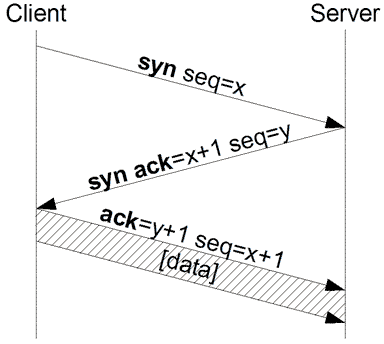
\includegraphics[scale=0.5]{images/300px-Tcp-handshake.png}
	\end{center}
	\caption{Beispiel eines TCP-Verbindungsaufbaus. Quelle: http://commons.wikimedia.org/wiki/File:300px-Tcp-handshake.png Lizenz: CC-BY-SA 3.0 Unported Autor: vermutlich Caos}
	\label{fig:impl:TcpHandshake}
\end{figure}

Beim SYN-Flooding jedoch sendet der Client niemals das abschließende ACK-Paket, sondern sendet weitere SYN-Pakete um noch mehr TCP-Verbindungen aufzubauen.
Dadurch zwingt der Angreifer den Server dazu, Informationen zu jeder noch nicht vollständig aufgebauten Verbindung zu speichern.
Da der zur Verfügung stehende Speicherplatz jedoch beschränkt ist, lässt sich damit die Verwaltung der Netzwerkverbindungen im Betriebssystem belasten. Arbeiten mehrere Angreifer zusammen, so kann man den Server hiermit überlasten.

\section{Andere DOS-Angriffe}
\index{DOS}
DDOS-Angriffe sind jedoch nicht die einzige Möglichkeit, einen Server lahmzulegen. Wir betrachten nun noch einen anderen beispielhaften Angriff, der technisch etwas interessanter ist.\\

Einige Sprachen, wie z.B. PHP, Python und JavaScript bieten die Möglichkeit Strings als Indizes von Arrays zu verwenden.
Wir haben dies bereits in unserem Beispiel zu SQL-Injection auf Seite \ref{listing:impl:SqlInjectionInPhp} gesehen. Dort wurde auf das (vordefinierte) Array \lstinline+$_GET+ zugegriffen. Dieses Array wird von PHP automatisch mit allen Parametern gefüllt, die der Client dem Server beim Aufruf einer Webseite per \lstinline+GET+-Methode übergibt. Z.B. wird bei der Anfrage
\begin{lstlisting}
http://www.example.com/?q=mad+magazine
\end{lstlisting}

der Wert "`\lstinline+mad magazine+"' unter dem Schlüssel "`\lstinline+q+"' in das (vordefinierte) Array \lstinline+$_GET+ eingefügt. Es ist also \lstinline+$_GET['q'] == 'mad magazine'+.

Intern wird hierfür eine Dictionary-Datenstruktur bzw. eine Hashtabelle verwendet.
Solchen Datenstrukturen liegt ein gewöhnliches (mit Zahlen indiziertes) Array $\overline{\texttt{\$\_GET}}$ der Länge $l$ sowie eine Hashfunktion $h$ zugrunde.
Um einen Wert $v_1$ (z.B. "'\lstinline+mad magazine+"') unter einem Index (oder Schlüssel) $s_1$ (z.B. "`\lstinline+q+"') zu speichern, wird der Schlüssel $s_1$ zunächst zu $h(s_1)$ gehasht.
Das Ergebnis wird modulo $l$ reduziert, und das Paar $(s_1, v_1)$ an der Position $h(s_1) \mod l$ im Array gespeichert.

Die Hashfunktion $h$ bietet jedoch keine kryptographische Kollisionsresistenz, da kryptographische Hashfunktionen zu aufwendig auszuwerten sind.
Deshalb kann es vorkommen, dass für ein zweites Schlüssel-Wert-Paar $(s_2, v_2)$ gilt, dass $h(s_2) \equiv h(s_1) \pmod l$ ist.
In diesem Fall müssen beide Paare $(s_1,v_1)$ und $(s_2,v_2)$ an der selben Stelle im Array gespeichert werden. Deshalb werden beide Paare üblicherweise in eine verkettete Liste eingefügt, die dann an dieser Stelle im Array $\overline{\texttt{\$\_GET}}$ gespeichert wird.%
\footnote{Eine Andere Strategie ist, $(s_2,v_2)$ an der nachfolgenden Stelle im Array zu speichern, sofern diese frei ist.}
Werden weitere Paare $(s_3, v_3), \ldots)$ mit $h(s_3) \equiv h(s_2) \pmod l$, \ldots, so werden diese Paare ebenfalls in die verkettete Liste eingefügt.\\

Tritt keine Hashkollision auf, so benötigt man für $n$ Zugriffe auf eine solche Dictionary-Struktur nur $\mathcal{O}(n)$ Operationen. Treten jedoch \emph{nur} Kollisionen auf, d.h. für alle $i,j$ gilt $h(s_i) \mod l = h(s_j) \mod l$, dann werden alle Elemente der Datenstruktur in \emph{nur einer} verketteten Liste gespeichert. Für $n$ Zugriffe werden dann $\Omega(n^2)$ Operationen benötigt.\\

Dies kann sich ein Angreifer zunutze machen. Da $h$ keine kryptographische Kollisionsresistenz bietet, kann der Angreifer eine große Anzahl entsprechender Schlüssel erzeugen, so dass diese in der Dictionary-Struktur des Servers alle in der selben Liste gespeichert werden. Dadurch kann der Angreifer gezielt eine hohe Last auf dem Server erzeugen.

Weitere Informationen zu diesem Angriff finden sich im Vortrag \cite{Klink2011}.


\backmatter

\nocite{*}
\bibliographystyle{plain}
\bibliography{literature}

\end{document}
